
\part*{Introduction}\label{part:intro}
    \chapter{Introduction}\label{chapter:intro}
        \glsresetall

\Gls{qm} is the study of nature's fundamental processes, manifest in its smallest particles. 
\gls{qm} has been at the forefront of physics since the early $20^{\textrm{th}}$ century \cite{jammer1966conceptual}.
Advances in theoretical understanding of quantum mechanical systems in the first half of the century 
    \cite{einstein1905heuristic, born1926quantenmechanik, schrodinger1926undulatory, heisenberg1985quantentheoretische, von2018mathematical}
    came to underpin many modern information and communications technologies\footnotemark \ in the second half
    \cite{svelto2010principles, van2004principles}.
The $21^{\textrm{st}}$ century, on the other hand, is poised to see the development of 
    technologies which \emph{deliberately} exploit the most intricate quantum processes \cite{feynman1982simulating}. 
These \emph{quantum technologies} share the promsie of super-classical outcomes,
    i.e. that exploiting quantum phenomena can yield results which could never 
    be achieved through non-quantum (or \emph{classical}) means.  
The enduring motivation for the development of quantum technologies is \emph{quantum simulation}:
    controlling quantum systems to represent other quantum systems, 
    enabling the study of such structures and interactions for the first time \cite{feynman1982simulating, lloyd1996universal}. 
\par 

\footnotetext{Colloquially referred to as \emph{Quantum 1.0}.}
\par 

Significant advances in the design and construction of quantum hardware in 
    recent years promise reliable, large scale quantum infrastructure
    in the near future \cite{arute2019quantum, zhong2020quantum}. 
Alongside improvements in quantum systems' control, progress in quantum algorithms and software 
    foreshadow impactful applications for quantum technologies, 
    from database search \cite{grover1997quantum} to quantum chemistry \cite{cao2019quantum} and drug design \cite{cao2018potential}.
Automated methodologies for characterising quantum systems are among the applications becoming feasible, 
    with the development of quantum devices capable of
    simulating nature at the quantum level \cite{childs2018toward}. 
There is a large and growing interest in automatically identifying the \emph{models} of quantum systems, 
    i.e. the mathematical structure representing a system's interactions
    \cite{rigo2020machine, cranmer2020discovering, bairey2019learning, pickard2011ab, chertkov2018computational}.
\par 

In parallel to the rise of quantum technologies over the past several decades,
    \gls{ml} and \acrlong{ai} have enjoyed increasing interest and resources.
Landmark outcomes, for example in facial recognition \cite{taigman2014deepface} 
    and complex strategy games \cite{silver2017mastering, brown2019superhuman},
    were bolstered by dramatic gains in the design of information processing machinery
    such as supercomputing facilities \cite{top500} and \acrlongpl{gpu} \cite{lindholm2008nvidia}.
\Gls{ml} has been widely adopted to accelerate the impact of quantum technologies, 
        from error correction \cite{chen2019machine, valenti2019hamiltonian}
        to metrology \cite{hentschel2010machine}
        and device calibration \cite{lennon2019efficiently}.
    
\par 

In this thesis we report progress in the domain of quantum system characterisation,
    through novel quantum algorithms empowered by the promise of quantum simulators, 
    leveraging state-of-the-art machine learning techniques. 
Namely, we introduce and develop the \gls{qmla} as a powerful platform for the study of 
    quantum systems, ranging from controlled quantum simulators to experimental setups.
\gls{qmla} distills an approximate model for a given quantum system, 
    by constructing a series of candidate models and testing them against data from the system of interest.
In providing a robust software framework for \gls{qmla}, we initiate an exciting field of research 
    at the overlap of \acrlong{ml} and quantum simulation, 
    with proposed applications in calibrating new quantum technologies as well as understanding 
    quantum processes in nature.

\section{Thesis outline}

The works presented in this thesis are closely related, 
    all stemming from the \gls{qmla} protocol and framework. 
The thesis is organised into \emph{parts}, 
    which group together related bodies of work;
    within each part, individual studies are presented in self contained chapters.
The main results and novel research is contained in \crefrange{part:algorithms}{part:experimental_study}.  
At the outset of each part, we summarise its chapters and contributions.
The contents of each part are as follows. 

\begin{description}
    \item[\cref{part:contextual_review} Contextual Review] \
    
        We introduce the concepts upon which the thesis will build. 
        \cref{chapter:qm} establishes the vocabulary of \acrlong{qm}, 
            followed by a summary of \acrlong{ml} in \cref{chapter:ml}. 
        In both cases, we seek to introduce the minimal nomenclature required to 
            contextualise the work in the following chapters;
            that is, neither topic is described exhaustively. 
    
    \item[\cref{part:algorithms} Algorithms] \
    
        We provide a thorough explanation of the algorithms underlying this thesis. 
        We start by summarising \acrlong{qhl}, which serves as a key subroutine within later studies and should therefore 
            be understood, in order that the contributions of later chapters may be fully appreciated.
        The first major result is the \gls{qmla} algorithm itself, 
            detailed in \cref{chapter:qmla}. 
        All subsequent chapters assume knowledge of the terminology and concepts related to \gls{qmla}, 
            so unfamiliar readers will find \cref{chapter:qmla} essential. 
        Our next contribution is an open source software platform for the implementation of \gls{qmla}, 
            for the study of arbitary quantum systems.
        In \cref{chapter:sw} we list the implementation details of this framework, 
            but do not further any physical or algorithmic concepts. 
        The \gls{qmla} software is available at \cite{flynn2021QMLA} with documentation at \cite{qmla_docs}.
        By the end of \cref{part:algorithms}, 
            we are armed with \gls{qmla} as a tool for the inspection of target quantum systems of interest,
            which will serve as a platform for the remaining chapters.
        
    
    \item[\cref{part:theoretical_study} Theoretical Study] \
    
        We perform tests of the \gls{qmla} framework under idealised simulated conditions, 
            corresponding directly to \cite{flynn2021Quantum}. 
        In \cref{chapter:lattices} we demonstrate that \gls{qmla} is trustworthy in the most straightforward scenario, 
            where a number of candidate models are proposed in advance. 
        We then move to more difficult conditions in \cref{chapter:ga}, 
            exploring spaces of $10^5$ valid candidate models, by incorporating a \acrlong{ga} within \gls{qmla}. 
        Together, the cases studied here verify that \gls{qmla} shows promise in characterising quantum systems, 
            in particular suggesting a compelling application in the calibration and verification of quantum simulators. 
    
    \item[\cref{part:experimental_study} Experimental Study] \

        The final contribution reflects work published in \cite{gentile2020learning}.
        We extend the \gls{qmla} protocol to \emph{realistic} quantum systems, namely targeting the decoherence processes dominating the 
        dynamics of an electron spin in a \acrlong{nvc}. 
        In \cref{chapter:nv} we operate on data extracted from an experimental system, 
            from which \gls{qmla} distills models with high predictive power -- i.e. which can reproduce the dynamics of the target system -- 
            and which are in agreement with theoretical predictions. 
        \cref{chapter:nv} relied on several constraints to facilitate the model search; 
            in \cref{chapter:many_qubits} we relax some of those constraints by simulating a similar system, 
            and again exploiting a \acrlong{ga} to explore the model space. 
        The results of this part indicate that \gls{qmla} may be helpful in the study of \emph{black-box} quantum systems.
    
    \item[\cref{part:conclusion} Conclusion] \
    
        We close the thesis with a brief summary of its main contributions, 
            and offer an outlook for model learning methodologies in the context of quantum technologies. 

\end{description}


\part{Contextual Review}\label{part:contextual_review}
    \chapter{Quantum Mechanics}\label{chapter:qm}
        \Gls{qm} -- the study of nature's fundamental processes, manifest in its smallest particles --
    has been at the forefront of physics since the early $20^{\textrm{th}}$ century \cite{jammer1966conceptual}.
Advances in theoretical understanding of quantum mechanical systems in the first half of the century 
    \cite{einstein1905heuristic, born1926quantenmechanik, schrodinger1926undulatory, heisenberg1985quantentheoretische, von2018mathematical}
    which came to underpin all modern information and communications technologies 
    \cite{svelto2010principles, van2004principles}.
The $21^{\textrm{st}}$ century, on the other hand, is poised to see the development of 
    technologies which \emph{deliberately} exploit the most intricate quantum processes in order to yield 
    some non-classical advantage. 
This thesis focuses on the application of \glsentrylong{ml} to the characterisation of quantum mechanical systems
    through use of quantum simulators, 
    so it is pertinent first to introduce the vocabulary of \gls{qm}. 
\footnotetext{Colloquially referred to as \emph{Quantum 1.0}.}
\par 

\Gls{qm} is central to the topics described in this thesis, 
    however it is impossible to succinctly capture the entire discipline; 
    in this chapter we will only introduce concepts utilised throughout.
For completeness, we elucidate some fundamental topics of linear algebra and quantum theory in \cref{apdx:fundamentals},
    but consider them too cumbersome to include in the main text. 
For a more complete and general introduction to \gls{qm}, the reader is referred to \cite{griffiths2018introduction, susskind2014quantum}.
Likewise, in this chapter we quickly summarise the key aspects of quantum computation, 
    but for further details, we recommend unfamiliar readers to consult \cite{rieffel2011quantum}, 
    while a more complete discussion is presented in \cite{nielsen2002quantum}.

%%%%%%%%%%%%%%%% QUANTUM MECHANICS %%%%%%%%%%%%%%%%%
\section{Quantum Mechanics}\label{sec:qm}

At any time, a quantum system, \gls{q}, can be described by its \emph{wavefunction}, $\Psi(t)$, 
    which contains all information about \gls{q}. 
In analogy with Newton's second law of motion, 
    which allows for the determination of a particle's position at any time, $\vec{r}(t)$, 
    given its conditions such as mass and acceleration as well as its initial position, $\vec{r}(t_0)$,  
    quantum \emph{equations of motion} can describe the evolution of \gls{q} through its wavefunction \cite{dirac1981principles}. 
One proposal\footnotemark \ for the equation of motion 
    to describe the evolution of the wavefunction under known conditions, 
    i.e. determining $\Psi(t)$ from $\Psi(t_0) \ \forall t > t_0$, 
    is \emph{\schrodinger's equation}  \cite{griffiths2018introduction, mart2020introduce, nelson1966derivation}.
\footnotetext{
    The most noteworthy alternative formalism, due to Heisenberg \cite{heisenberg1985quantentheoretische}, 
    was shown equivalent to the \schrodinger picture described here.
}
\par 

Although the \schrodinger equation is a \emph{postulate} of \gls{qm} (see \cref{sec:postulates}), 
    let us introduce it in reverse order to elucidate its meaning, following \cite{susskind2014quantum}. 
We have yet to describe the structure of the wavefunction, which we will do in \cref{sec:quantum_info},
    but here we will represent wavefunctions using \emph{Dirac notation} (\cref{sec:dirac_notation}), 
    and can think of them generically as vectors, i.e. $\Psi(t) \rightarrow \ket{\psi(t)}$. 
Suppose we have two such wavefunctions, $\ket{\phi(t)}, \ket{\psi(t)}$ which are functions of time $t > t_0$.
We start with the assumption that \emph{similarity} is conserved between two wavefunctions,
    if they undergo the same transformation 
    (Susskind's \emph{minus first} law of classical mehcanics \cite{susskind2014quantum})
\begin{equation}
    \label{eqn:conservation_simularity}
    \braket{\phi(t) | \psi(t)} = \braket{\phi(t_0) | \psi(t_0)}
\end{equation}

Then, assuming some equations of motion capture the dynamics of \gls{q}, 
    there exists some evolution operator, $\hat{U}(t)$, which deterministically maps $\ket{\psi(t_o)}$ to $\ket{\psi(t)}$.
\begin{equation}
    \label{eqn:unitary_time_evolution}
    \ket{\psi(t)} = \hat{U}(t) \ket{\psi(t_0)},
\end{equation}
    where we have not yet imposed any restrictions on $\hat{U}$. 
Combining \crefrange{eqn:conservation_simularity}{eqn:unitary_time_evolution}, 
\begin{equation}
    \begin{split}
        \braket{\phi(t) | \psi(t)} &= \braket{ \phi(t_0) | \hat{U}^{\dag} \hat{U}| \psi(t_o) }
        \\
        \Rightarrow \braket{ \phi(t_0) | \hat{U}^{\dag}(t) \hat{U}(t) | \psi(t_o) } &= \braket{\phi(t_0) | \psi(t_0)}
        \\
        \Rightarrow \hat{U}^{\dag}(t) \hat{U}(t) &= \ident \ \ \ \ \forall t,
    \end{split}
\end{equation}
where the result $\hat{U}^{\dag}(t) \hat{U}(t) = \ident$ is the condition for \emph{unitarity} (\cref{sec:unitary}), 
    so we can claim the quantum wavefunction evolves unitarily. 
\par 

By construction, we require that after zero time, i.e. $t = t_0$, the wavefunction has not changed:
\begin{equation}
    \begin{split}
        \ket{\psi(t = t_0)} = \hat{U}(t = t_0)\ket{\psi(t_0)} = \ket{\psi(t_0)}
        \\ \Rightarrow \hat{U}(t = t_0) = \ident.
    \end{split}
\end{equation}
Without loss of generality we can set $t_0 = 0$, giving $\hat{U}(0) = \ident$. 
Then, let us consider an infintesimally small time increment $t_0 + \epsilon$:
    again, take $t_0 = 0$ so $t = \epsilon$,  where $\epsilon \gg \epsilon^2$. 

We can say
\begin{equation}
    \hat{U}(\epsilon) = \ident + \mathcal{O}(\epsilon),
\end{equation}
which merely suggests that the time evolution operator
    at very small time is very close to the identity, with some small displacement proportional to the time,
    which must be an operator to act on the wavefunction (vector).
We suppose the form of the offset, so we can write
\begin{equation}
    \hat{U}(\epsilon) = \ident - \epsilon \left(\frac{i}{\hbar} \ho \right),
\end{equation}
    where the inclusion of the phase $-i$ is arbitrary, 
    and we have named as $\nicefrac{\ho}{\hbar}$ the operator by which the time evolution differs from the identity. 
In other words, the operator $\ho$ is generically the generator of the evolution/dynamics of \gls{q}:
    any difference between $\ket{\psi(t_0)}$ and $\ket{\psi(t)}$ arises solely due to $\ho$. 
So far there is no restriction on $\ho$, 
    except that it must be of the same dimension as the Hilbert space in question. 
Recalling the unitarity condition, however:
\begin{equation}
    \label{eqn:hamiltonian_hermiticity}
    \begin{split}
        \hat{U}^{\dag}(\epsilon) \hat{U}(\epsilon) &= \ident
        \\ 
        \Rightarrow 
        \left( \ident + \frac{i}{\hbar} \epsilon \ho^\dag \right) \left( \ident - \frac{i}{\hbar} \epsilon \ho, \right)  &= \ident
        \\
        \Rightarrow
        \ident +  \frac{i}{\hbar} \epsilon (\ho^{\dag} - \ho) + \mathcal{O}(\epsilon^2) &= \ident
        \\
        \Rightarrow
        (\ho^{\dag} - \ho) = 0 
        \\
        \Rightarrow
        \ho^{\dag} = \ho.
    \end{split}
\end{equation}
\cref{eqn:hamiltonian_hermiticity} results in the condition for \emph{Hermiticity}, 
    meaning that $\ho$ is an observable of \gls{q}. 
In fact, this is the \emph{Hamiltonian} of the system, described in the next section. 

\par 
We can also use the infintesimal evolution to see 
\begin{equation}
    \label{eqn:derivation_schrodinger_eqn}
    \begin{split}
        \ket{\psi(t)} &= \hat{U}(t) \ket{\psi(t_0)}
        \\ \Rightarrow \ket{\psi(\epsilon)} &= \hat{U}(\epsilon) \ket{\psi(t_0)}
        \\ \Rightarrow 
        \ket{\psi(\epsilon)} &= \left(\ident - \epsilon \frac{i}{\hbar} \ho \right) \ket{\psi(t_0)}
        \\ \Rightarrow \ket{\psi(\epsilon)} &= \ket{\psi(t_0)} - \epsilon \frac{i}{\hbar} \ho \ket{\psi(t_0)}
        \\ \Rightarrow \frac{\ket{\psi(\epsilon)} - \ket{\psi(t_0)} }{\epsilon}  &= - \frac{i}{\hbar} \ho \ket{\psi(t_0)}
    \end{split}
\end{equation}
Taking the limit as $\epsilon \rightarrow 0 $, the left hand side of the final line of \cref{eqn:derivation_schrodinger_eqn} is the definition
    of the derivative of the wavefunction, $\frac{d \ket{\psi(t)}}{dt}$. 
Taken together, we have 
\begin{equation}
    \label{eqn:schrodinger}
    \frac{d}{dt} \ket{\psi(t)} = \frac{-i}{\hbar} \ho \ket{\psi(t_0)},
\end{equation}
    where $\ket{\psi(t)}$ is the wavefunction at time $t$, 
    $\ket{\psi(t_0)}$ is the wavefunction at $t_0$, such that $t > t_0$, 
    $\hbar = 1.054 \times 10^{-34}$ is the reduced Planck constant and 
    $\ho$ is the \emph{Hamiltonian} of \gls{q}. 
For brevity we generally refer to $t_0 = 0$, and absorb $\hbar$ into $\ho$, which will later manifest in the Hamiltonian scalar parameters. 
\cref{eqn:schrodinger} is the most general form of \emph{\schrodinger equation}, 
    otherwise known as the \emph{time-dependent} \schrodinger equation; 
    we include it as \Cref{postulate:schrodinger_eqn} when describing the fundamentals of \gls{qm} (\cref{sec:postulates}), 
    since it can be seen as an irreducible equation of motion which is essential to the description of quantum systems. 
\par 

As mentioned, we presented this argument in a nonstandard order:
    we started with \cref{eqn:unitary_time_evolution}, which we can now consider the \emph{solution} to the \schrodinger, 
    specifically
\begin{equation}
    \label{eqn:unitary_evolution}
    \begin{split}
        \ket{\psi(t)} = \hat{U}(t) \ket{\psi(0)}
        \\
        \hat{U}(t) = e^{-i \ho t} 
    \end{split}
\end{equation}
    which describes the unitary evolution of the state according to the unitary evolution operator, $\hat{U}(t)$. 
\par 

\subsection{Hamiltonians}\label{sec:hamiltonians}
In the previous section we introduced the Hamiltonian\footnotemark \ of \gls{q} as the generator of its 
    time evolution dynamics;
    Hamiltonians are of primary importance in this thesis, so it is worth pausing to consider their physical meaning. 
We saw in \cref{eqn:hamiltonian_hermiticity} that $\ho$ is Hermitian, 
    meaning that the operator is physically observable 
    according to \Crefrange{postulate:eigenvalues}{postulate:hermiticity}
    of \glsentrylong{qm} (\cref{sec:postulates}). 
The Hamiltonian operator captures the energy of \gls{q}: 
    the eigenvalues of the observable $\ho$ are the permitted energy levels of the system.
\par 

The quantum Hamiltonian, $\ho$, is analogous to the classical Hamiltonian, 
    insofar as it captures all the interactions of a given system which contribute to its time evolution.
Knowing the classical Hamiltonian and the initial conditions -- position and momentum -- 
    Hamilton's equations of motion allow for the calcaultion of those quantities for the particle 
    in question an infintesimal time later \cite{susskind2014classical}.    
Likewise, knowledge of the initial wavefunction, $\ket{\psi(t_0)}$, and the system's quantum Hamiltonian, $\ho$, 
    the quantum equations of motion -- \schrodinger's equation, \cref{eqn:schrodinger} -- 
    permits the calculation of the wavefunction at later times.
As such the Hamiltonian must consist of all processes which influence the evolution of \gls{q};
    we will later break the Hamiltonian into independent \emph{terms} which each correspond to unique physical interactions
    \gls{q} is subject to, \cref{sec:models}. 
We can think that each process/interaction \gls{q} undergoes contributes to its total energy,
    giving intuition as to why its eigenvalues are the energy levels. 
\par 
\footnotetext{
    Aside: the author shares a hometown with the mathematician for whom it is named, William Rowan Hamilton. 
    It is hoped that, after another 150 years, the next physicist from Trim, Co. Meath, Ireland might 
    profitably use knowledge of Hamiltonians on a \gls{qc}. 
}

Hamiltonians describe \emph{closed} quantum systems, 
    i.e. where \emph{all} processes and interactions which influence \gls{q} are accounted for. 
Realistic quantum systems are influenced by a myriad of proximal systems, 
    and it is therefore infeasible to analytically account for them all. 
Instead, \emph{open} quantum systems' dynamics are described by Lindbladian operators, which encompass the Hamiltonian form. 
The Lindblad master equation is a generalisation of the \schrodinger equation, 
    providing the equation of motion for open quantum systems \cite{breuer2002theory, manzano2020short}.
In this thesis we only consider closed models for quantum systems;
    for meaningful impact of the techniques presented here, it will be necessary to expand them to account for the open system dynamics of realistic experiments.
We do, however, show initial progress towards this endeavour by modelling a physical system through a closed Hamiltonian, \cref{chapter:nv}.
\par 

%%%%%%%%%%%%% QUANTUM INFORMATION %%%%%%%%%%%%%
\section{Quantum Information}\label{sec:quantum_info}
We have not yet described the structure of the wavefunction, 
    instead performing the previous analysis with respect to some arbitrary objects.
The wavefunction for a physical system, \gls{q}, is also known as its \emph{state}, 
    a complete mathematical description of the system \cite{preskill1998lecture}.
States are vectors\footnotemark, $\ket{\psi} \in \mathbb{C}$;
    the valid state space for \gls{q} is its \emph{Hilbert space}, $\hilbert$,
    which is a generalisation of Euclidean vector space, 
    i.e. $\ket{\psi} \in \hilbert$. 
\footnotetext{We immediately use Dirac notation to represent the state; it is defined in \cref{sec:dirac_notation}.}
The Hilbert space defines the overlap between any two vectors as the \emph{inner product}, $\braket{\psi | \phi}$ (\cref{sec:linear_algebra}). 
In general\footnotemark, a state can be seen as a \emph{superposition} across its eigenstates, $\left\{\ket{v_i}\right\}$.  
\footnotetext{We expand on this brief description in \cref{sec:states}.}

\begin{subequations}
    \begin{equation}\label{eqn:state_vector}
        \ket{\psi} = \sum\limits_{i} \alpha_i \ket{v_i}
    \end{equation}
    \begin{equation}\label{vector_norm}
        \textrm{subject to} \ \ \ \sum\limits_{i} |\alpha_i|^2 =1, \ \ \ \alpha_i \in \mathbb{C}. 
    \end{equation}
\end{subequations}

The cornerstone of \gls{qm} is the effect of \emph{measurement} on quantum systems: 
    in general \gls{q} can be seen as occupying a multitude of eigenstates as in \cref{eqn:state_vector};
    observing the system forces $\ket{\psi}$ into a definite occupation of a single eigenstate,
    where the \emph{probability} that it is measured in each eigenstate $\ket{v_i}$ is given by $\absval{\alpha_i}^2$, 
    according to Born's rule \cite{born1926quantenmechanik}.
$\alpha_i$ are hence named \emph{probability amplitudes} since they inform the probability of measuring the corresponding eigenstate. 
\par 

For an ideal\footnotemark \ single particle, when the state, \cref{eqn:state_vector}, has two available eigenstates, 
    e.g. the horizontal ($H$) and vertical ($V$) polarisation of a single photon, 
    we can designate \gls{q} as a two-level computational platform, called a \emph{qubit}, 
    analogous to the workhorse of classical computation, the bit. 
A qubit's state vector can then be written as a sum over the two available eigenstates, 
    where we assign vectors to the eigenstates as $\left\{ \ket{H} = \ket{v_1}, \ket{V} = \ket{v_2} \right\}$. 
\footnotetext{
    Here we restrict to the space of ideal, \emph{logical} qubits. In reality, physical qubits are beset by errors, 
    demanding error correction routines such that multiple particles are needed attain a single logical qubit. 
}
\begin{equation}
    \label{eqn:qubit_state}
    \ket{\psi} = \alpha_1 \ket{v_1} + \alpha_2 \ket{v_c},
\end{equation}
where $\alpha_i \in \mathbb{C}$ and $\absval{\alpha_1}^2 + \absval{\alpha_2}^2 = 1$. 
\par

In general, a qubit requires two orthogonal state vectors to define a \emph{basis};
    we list a number of the usual special cases:
\begin{subequations}
    \label{eqn:bases}
    \begin{equation}
        \label{eqn:basis_x}
        X\textrm{-basis} = \left\lbrace \begin{split}
        \ket{+} &= \frac{1}{\sqrt{2}} \left( \ket{0} + \ket{1} \right)
        \\
        \ket{-} &= \frac{1}{\sqrt{2}} \left( \ket{0} - \ket{1} \right)
        \end{split}
        \right.
    \end{equation}
    \begin{equation}
        \label{eqn:basis_y}
        \begin{split}
        Y\textrm{-basis} = \left\lbrace 
        \begin{split}
            \ket{i} &= \frac{1}{\sqrt{2}} \left( \ket{0} + i \ket{1} \right)
            \\
            \ket{-i} &= \frac{1}{\sqrt{2}} \left( \ket{0} - i \ket{1} \right)
        \end{split}
        \right.        
        \end{split}
    \end{equation}
    \begin{equation}
        \label{eqn:basis_z}
        Z\textrm{-basis} = \left\lbrace \begin{split}
            &\ket{0}
            \\
            &\ket{1}
            \end{split}
            \right.
    \end{equation}
\end{subequations}

A visual tool for representing qubits is the \emph{Bloch sphere}, 
    which presents orthogonal basis states as parallel unit vectors of opposite direction:
    we show each of the bases of \cref{eqn:bases} in \cref{fig:bases}. 

\begin{figure}
    \begin{center}
        \subfloat{
            % 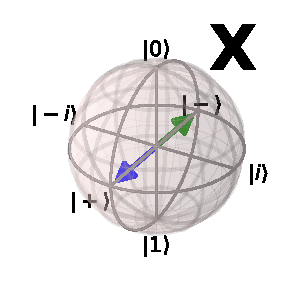
\includegraphics[width=0.3\textwidth]{contextual_review/figures/bloch_x_axis.pdf}
            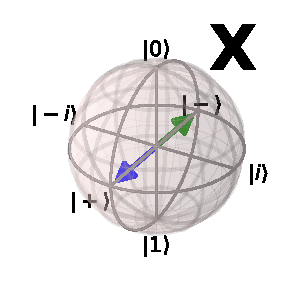
\includegraphics{contextual_review/figures/bloch_x_axis.pdf}
        }
        \qquad
        \subfloat{
            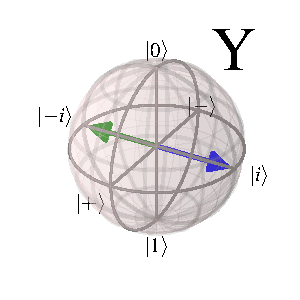
\includegraphics{contextual_review/figures/bloch_y_axis.pdf}
        }
        \qquad
        \subfloat{
            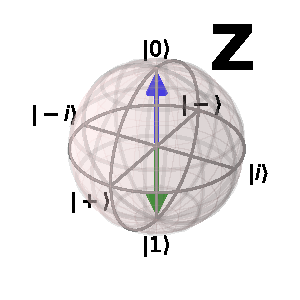
\includegraphics{contextual_review/figures/bloch_z_axis.pdf}
        }
        \qquad
    \end{center}
    \caption[Bloch sphere representation of bases]{
        Bloch sphere representation of bases, where each pair of basis states are shown by blue and green vectors. 
        The $X$-basis has basis vectors $\left\{ \ket{+}, \ket{-}\right\}$; $Y$-basis has $\left\{ \ket{i}, \ket{-i}\right\}$ 
            and $Z$-basis has $\left\{ \ket{0}, \ket{1}\right\}$.
    }
    \label{fig:bases}
\end{figure}

We can make two remarks about basis states for a single qubit:
\begin{easylist}[itemize]
    & Basis states from one basis can be seen as superpositions with respect to alternative bases
    && e.g. in the $X$-basis, $\ket{+}$ is a basis vector, but in the $Z$-basis, $\ket{+} = \frac{\ket{0} + \ket{1}}{\sqrt{2}}$ is a superposition over basis vectors. 
    & Bases are local rotations of each other
    && rotating the $X$-basis through an angle $\nicefrac{\pi}{2}$ about the $Y$-axis results in the $Z$-axis.
\end{easylist}

\par 

As we alluded to in \cref{sec:qm}:
    by imposing mathematical structure on quantum systems' states, 
    i.e. representing \gls{q} as a state vector at any time, 
    then operations which alter the state of the system must be matrices, 
    which we will call \emph{operators}. 
In general an $n$-dimensional vector is rotated by an $n \times n$ matrix;
    therefore to rotate the one-qubit state, given by a two-dimensional vector, 
    we require a $2\times2$ operator.
One-qubit operators have the effect of rotating the state vector, 
    which we can again visualise on the Bloch sphere.
By thinking of qubits generically with respect to any basis, we can encode information in the qubit's amplitudes,
    by performing operations (or \emph{gates}) upon the qubit, we change the information, 
    i.e. we can design information processing techniques leveraging the infrastructure -- states, operators and measurement -- of \gls{qm}. 
\par 

We introduce a set of speical one-qubit operators, the \emph{Pauli matrices},  

\begin{subequations}
    \begin{equation}
        \sx = \begin{pmatrix}
            0 & 1 \\
            1 & 0 
        \end{pmatrix}
    \end{equation}        
    \begin{equation}
        \sy = \begin{pmatrix}
            0 & -i \\
            i & 0 
        \end{pmatrix}
    \end{equation}        
    \begin{equation}
        \sz = \begin{pmatrix}
            1 & 0 \\
            0 & -1 
        \end{pmatrix}
    \end{equation}        
\end{subequations}

The Pauli matrices are used to define rotation operators about 
    their respective axes, and hence are very useful:
    we can break \emph{any} rotation of a qubit into rotations of various angles, $\theta$, about the three axes of the Bloch sphere.
Any single qubit operation can therefore be expressed as a product of
    the \emph{rotation operators}, $\hat{R}_x, \hat{R}_y, \hat{R}_z$, exemplified in \cref{fig:bloch_rotations} and defined for $w \in \{ x,y,z\}$ as
\begin{equation}
    \label{eqn:rotation_operator}
    \begin{split}
        \hat{R}_w\left(\theta\right) &= e^{-i \frac{\theta}{2} \hat{\sigma}_w} 
        = \cos\left(\nicefrac{\theta}{2}\right) \ident - i \sin \left(\nicefrac{\theta}{2}\right) \hat{\sigma}_w.
    \end{split}
\end{equation}
    
\par
The Pauli matrices are Hermitian, meaning they are observable. 
We can see that the eigenstates of $\sz$ are the $Z$-basis states:
    $\sz \ket{0} = \ket{0}; \sz \ket{1} = - \ket{1}$.
Recalling the earlier claim that the two-level quantum system (e.g. $H$ and $V$ polarisation of a photon)
    can be mapped to eigenvectors\footnotemark \ of an obserable operator to form a qubit, 
    we term the $Z$-basis the \emph{computational} basis.
By defining the computational basis, we ground abstract computational reasoning in the physical realisation:
    anywhere throughout this thesis where the basis states $\ket{0}, \ket{1}$ are referenced, 
    we mean the eigenstates of the physical axis which is defined as the $Z$-axis for the system in question. 
\footnotetext{
    The terms \emph{eigenstate} and \emph{eigenvector} are interchangeable, 
    although it may be helpful to think of eigenstate as the physical manifestation (horizontal photon), 
    and think of eigenvector as the logical manifestions ($\ket{0}$). 
}
In the computational basis, then, a qubit can be specified as
\begin{equation}
    \label{eqn:computational_qubit}
    \ket{\psi} = \alpha_0 \ket{0} + \alpha_1 \ket{1}.
\end{equation}

\begin{figure}
    \begin{center}
        \subfloat{
            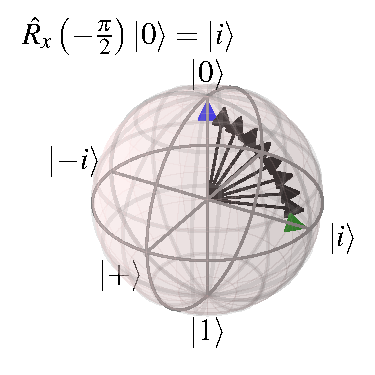
\includegraphics{contextual_review/figures/bloch_rotate_x.pdf}
        }
        \qquad
        \subfloat{
            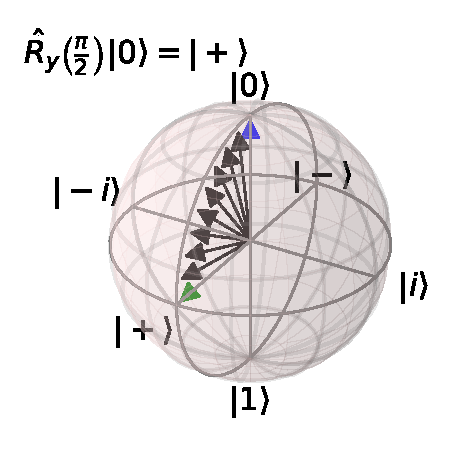
\includegraphics{contextual_review/figures/bloch_rotate_y.pdf}
        }
    \end{center}
    \caption[Rotations on Bloch sphere]{
        Rotations on Bloch sphere. 
        The initial and final state are shown in blue and green respectively, while intermediate states are shown in black. 
        \textbf{Left}, The $Z$-basis unit vector, $\ket{0}$, is rotated about the $X$-axis, resulting in the unit vector along the $Y$-axis. 
        \textbf{Right}, The $Z$-basis unit vector, $\ket{0}$, is rotated about the $Y$-axis, resulting in the unit vector along the $X$-axis. 
    }
    \label{fig:bloch_rotations}
\end{figure}
\par 

The concepts of qubits representing quantum systems, as well as operators
    altering their states and measurement collapsing those states,
    extend straightforwardly to multipartite systems, by merging Hilbert spaces through tensor products, 
    as we show in \cref{sec:multipartite}. 
The cases where this is a simple mathematical exercise represent \emph{pure} states;
    of course this leads to the more intricate topic of \emph{mixed} states and entanglement, 
    briefly described in \cref{sec:entanglement}.
In this thesis, however, we are concerned only with pure states, i.e. separable qubits.
While single qubit states are spanned by the Pauli opeartors, multi-qubit states are spanned by the Pauli group, $\mathbb{G}$: 
    $n$-qubit states are spanned by $\mathbb{G}_n = \left(\mathbb{C}^2\right)^{\otimes n}$.

\subsection{\Gls{expectation value}}\label{sec:expectation_value}
\begin{figure}
    \begin{center}
        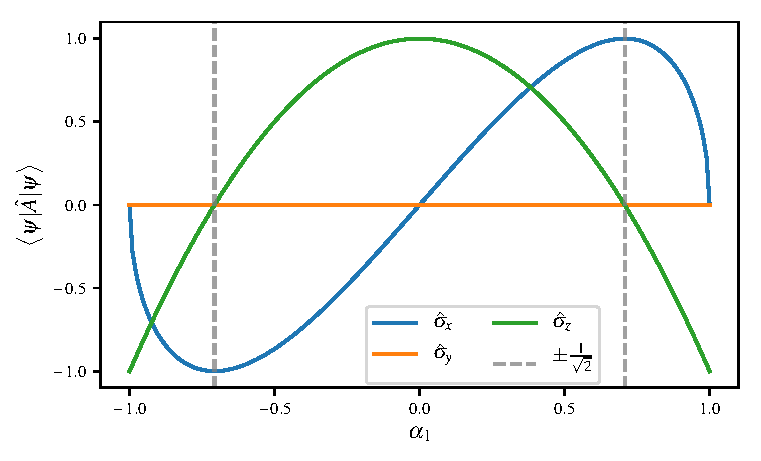
\includegraphics{contextual_review/figures/expectation_values.pdf}
    \end{center}
    \caption[Expectation values]{
        Expectation values of the observable $\hat{A}$ -- here the Pauli matrices --  
            for $\ket{\psi} = \alpha_0 \ket{0} + \alpha_1 \ket{1}$.
            Coefficients are real, varying $\alpha_1 \in \left( -1, 1\right)$, such that $\alpha_0 = \sqrt{1 - \alpha_1^2}$. 
    }
    \label{fig:expectation_values}
\end{figure}

Upon measurement, the state vector of \gls{q} has amplitude associated with only one eigenvector. 
On average, however, the eigenvector to which it would collapse encodes statistical insight on the 
    state prior to measurement. 
In other words, if we prepared $\ket{\psi}$ and measured it -- via some observable, $\hat{A}$ -- 
    and repeat the procedure $N$ times, 
    then as $N \rightarrow \infty$, the average outcome is the \emph{expecatation value}
    for the system is given by 
\begin{equation}
    \label{eqn:expectation_value}
    \braket{\hat{A}} = \braket{\psi | \hat{A} | \psi} = \sum\limits_{i} \alpha_i \braket{v_i | \hat{A} | v_i},  
\end{equation}
    where $\braket{\hat{A}}$ is the \gls{expectation value} (average) for the observable, $\hat{A}$; 
    $\ket{v_i}$ are the eigenvectors of $\hat{A}$, and $\alpha_i \in \mathbb{C}$ are the proability amplitudes
    associated with each $\ket{v_i}$ when the state $\ket{psi}$ is represented as in \cref{eqn:state_vector}.
We show some examples of \glspl{expectation value} for the observable Pauli matrices in \cref{fig:expectation_values}. 
\par 

An underlying theme of this thesis is to flip the usual logic: 
    instead of using knowledge of the system to derive the \gls{expectation value}, per \cref{eqn:expectation_value},
    we will \emph{estimate} \glspl{expectation value}, either through experiment or simulation, 
    and use them to infer the structure of the observable.
This trick enables machine learning routines to reverse engineer 
    the processes \gls{q} is subject to, as we will describe in \cref{part:algorithms}. 
There is a subtlety to be aware of, however: 
    in later chapters, we will make reference to the \gls{expectation value} and \emph{\gls{likelihood}} 
    almost interchangeably -- these are distinct concepts that \emph{sometimes} overlap, but not in all cases,
    as we explain in \cref{chapter:qhl}. 


%%%%%%%%%%%%%%% QUANTUM COMPUTING %%%%%%%%%%%%%%%%%%

\section{Quantum Simulation and Computation}

Relying on the premise and language of quantum information processing 
    -- states, qubits, operators, measurements and expectation values -- 
    the growing field of \emph{quantum technology} aims to exploit the 
    non-classical statistics yielded by quantum systems in order to retrieve 
    outcomes beyond the capability of their classical counterparts \cite{dowling2003quantum}. 
Applications range from enhanced sensing and metrology \cite{giovannetti2004quantum, giovannetti2011advances}, 
    to highly-secure communication and cryptography protocols \cite{bennett2020quantum, ekert1991quantum, gisin2002quantum}.
The initial motivation for the development of quantum technologies, however, 
    was the  observation that simulating nature at a quantum level would require 
    exponential resources and is therefore only feasible given controllable quantum systems,
    which can accurately emulate the true dynamics \cite{manin1980vychislimoe, benioff1980computer, benioff1982quantum, feynman1982simulating}. 

\par 
The notion of controlling quantum systems to mimic the dynamics of real quantum systems is tantamount to 
    \emph{quantum simulation} \cite{lloyd1996universal, cirac2012goals}. 
In particular, simulating quantum systems is believed to be of interest for quantum chemistry \cite{lanyon2010towards, cao2019quantum, mcardle2020quantum}, 
    for example leading to advances in the simulation of molecular dynamics \cite{aspuru2005simulated, sparrow2018simulating}.
More generally, however, this led to research into a wider domain of calculations called \emph{quantum computation}
    which considers the information processing capability of controllable quantum systems beyond merely simulating quantum systems. 
Then, \emph{universal \glsentrylongpl{qc}} (or, \emph{quantum Turing machines}), 
    assume access to \emph{logical} qubits and operations (or \emph{gates}) for the implementation of quantum circuits \cite{deutsch1985quantum}. 
This ignited interest in \emph{quantum algorithms}, which aim to provide some provable advantage 
    \cite{simon1997power, bennett1997strengths, bernstein1997quantum, grover1997quantum, shor1999polynomial}.
Indeed, it was found that the space of problems addressible by such devices
    goes beyond the classical counterpart,
    suggesting there exists a class of quatum algorithms which can offer significant advantage over 
    any feasible algorithm on classical hardware \cite{watrous2008quantum}. 
\par 

Of course, while the advances in algorithmic quantum computation promise huge impact, 
    they are tempered by contemporary experimental constraints, 
    which must deal with the reality that construction and control of 
    quantum devices is a significant challenge.
In constructing \glspl{qc} and dealing with their output, 
    we must account for physical effects which lead to errors, 
    requiring expensive error mitigation schemes to be reliable \cite{shor1996fault, aharonov2008fault}.
Furthermore, there are a number of criteria a \gls{qc} must meet before it can be deemed reliable \cite{divincenzo2000physical}. 
\par 

Any two-level quantum system can be used as a qubit;
    a range of platforms have emerged in attempts to fulfil the potential of quantum computation \cite{humble2019quantum},
    among the most popular\footnote{An incomplete list of quantum architectures together with their primary advantages and limitations.}:

\begin{easylist}[itemize]
    & Photonic qubits (linear optical \glspl{qc}) \cite{kok2007linear}
    && existing infrastructure for commercial production of photonics-based technologies suggests the relatively straightforward fabrication 
        of integrated photonic devices at the scale of millions of degrees of freedom \cite{adcock2020advances};
    && photons do not decohere so are useful for encoding information \cite{kovac2002detection};
    && photons do not interfere \cite{dirac1981principles, gerry2005introductory}, 
        so information processing must be mediated by non-trivial measurement schemes \cite{raussendorf2003measurement};
    && they are liable to a unique error mechanism -- photon loss -- 
        necessitating novel quantum error correcting codes \cite{vigliar2020error};
    && on-demand single photon generation has not yet been demonstrated,
        although there is significant progress in the area of photon generation \cite{paesani2020near}.

    & Superconducting qubits \cite{devoret2004superconducting, kjaergaard2020superconducting}
    && relatively straightforward to control and couple with each other, enabling high-fidelity two-qubit gates,
        e.g. $99.7 \%$ reached in \cite{kjaergaard2020quantum};
    && difficult to engineer substantial coherence times, although there has been significant recent progress 
        \cite{martinis2014ucsb, wendin2017quantum},
        e.g. $T_1 \sim \mathcal{O}(\textrm{ms})$ in \cite{pop2014coherent};
    && require cryogenic temperatures \cite{devoret2004superconducting};
    && arbitrary qubit connectivity at scale is yet to be demonstrated \cite{kjaergaard2020superconducting};
    && methods for the fabrication of medium-to-large scale devices required for fault tolerant 
        quantum computation are not yet known \cite{gambetta2017building}.

    & Ion traps \cite{kielpinski2002architecture, monroe2013scaling}
    && high two qubit gate fidelities, e.g. $99.9\%$ in \cite{gaebler2016high};
    && very high coherence times, e.g. $\mathcal{O}(10 \ \textrm{min})$ in \cite{wang2017single};
    && straightforward state preparation and readout, e.g. $99.99\%$ readout fidelity in \cite{myerson2008high};
    && long gate-times, e.g. $\mathcal{O}(\mu \textrm{s})$ in \cite{schafer2018fast};
    && uncertain scalability \cite{bruzewicz2019trapped}.

\end{easylist}
\par 

The ever-increasing space of contenders has led to a growing eco-system for quantum software \cite{larose2019overview},
    promising a wide range of applications in the era of noisy intermediate scale quantum devices \cite{preskill2018quantum}. 
Following numerous proposoals \cite{harrow2017quantum},
    recent efforts have married state-of-the-art hardware with bespoke algorithms in order to achieve quantum advantage
    \cite{arute2019quantum, zhong2020quantum}. 
Evidently there is vast effort in bringing quantum computational resources to reality; 
    in this thesis, however, we are not concerned with the architecture underlying our presumed quantum simulator -- 
    we perform simulations only on classical hardware. 
In principle, however, any quantum simulator -- universal or otherwise -- capable of implementing the time evolution 
    operator, \cref{eqn:unitary_evolution}, can be called upon as a co-processor by the algorithms presented. 
\par 

Our restriction to classical resources leads to a few remarks:
\begin{easylist}[itemize]
    & given access to a fault-tolerant \gls{qc}/simulator,
        the algorithms described would enjoy an automatic exponential speedup:
    && the classical bottleneck is the calculation of the time evolution dynamics, 
        \cref{eqn:unitary_evolution}, according to the matrix exponential, of dimension $2^n$, 
        where $n$ is the dimension of the system;
    && it is believed that the same calculation can be performed in polynomial time on a \gls{qc} \cite{lloyd1996universal}. 

    & the results achieved in this thesis are limited by the capability of classical computers in simulating quantum systems
    && we study only up to 8-qubit systems, whereas it would be of interest to extend these methods to higher dimensions, 
        which is expected to be feasible when reliable quantum simulators/computers are available.
\end{easylist}

The remit of this thesis -- given these limitations --
    is therefore to robustly test the presented algorithms,
    and provide a benchmark achieved through classical facilities, 
    against which the same algorithm can be run in conjunction with quantum hardware. 

\par 
    \chapter{Machine Learning}\label{chapter:ml}
        \Gls{ml} is the application of statistics, algorithms and computing power to discover meaning and/or devise actions from data.
\gls{ml} has become an umbrella term, encompassing the family of algorithms
    which aim to leverage computers to learn without being explicitly programmed,
    as opposed to the more general \gls{ai}, which seeks to make computers behave intelligently,
    admitting explicit programs to achieve tasks \cite{MLvAI}.
Its history is therefore imprecise since a number of early, apparently unrelated algorithms were proposed independently, 
    which now constitute \gls{ml} routines \cite{mcculloch1943logical, turing2009computing}. 
Nevertheless, the field of \gls{ml} has been advancing rapidly since the second half of the $20^{\textrm{th}}$ century \cite{russell2002artificial}, 
    especially recently due to the availability of advanced hardware such as \glspl{gpu}, 
    facilitating significant progress through an ever-increasing aresnal of powerful open source software \cite{pedregosa2011scikit, abadi2016tensorflow, paszke2019pytorch}. 
\par 

Throughout this thesis, we endeavour to combine known methods from the \gls{ml} literature with capabilities of \glspl{qc}\footnotemark. 
Typical \gls{ml} algorithms, which rely on \glspl{cpu} or \glspl{gpu}, are deemed \emph{classical} \glsentrylong{ml},
    in contrast with \gls{qml}, where \glspl{qc} are central to processing the data.
Similarly to the remit of \cref{chapter:qm}, here we do not provide an exhaustive account of \gls{ml} algorithms:
    rather, we describe only the algorithms which are used in later chapters, 
    referring readers to standard texts for a wider discussion \cite{russell2002artificial, hastie2009elements}.

\footnotetext{Or simulated \glspl{qc}, in this thesis.}


\section{Classical \glsentrylong{ml}}\label{sec:classical_ml}

Of course the first step in any \gls{ml} application is to consider the types of available data,
    with respect to the ensemble of known algorithms. 
Classical \gls{ml} is usually described in three categories,
    broadly based on the format of data on which the insight can be built;
    we will briefly describe each to provide context to discussions throughout this thesis. 
Later in this thesis we will use the word \emph{model} for descriptions of quantum systems, 
    but here \emph{model} refers to the mapping between inputs and outputs which the \gls{ml} algorithm devises.
\par 

\subsection{Supervised \glsentrylong{ml}}
Models are trained using \emph{labelled} data, 
    i.e. each training sample has a known label $y_i$;
    or, a set of \emph{feature vectors} $\left\{\vec{x}_i\right\}$ are associated with the set of 
    corresponding \emph{classes} $\left\{ y_i \right\}$ \cite{caruana2006empirical}. 
The output is a predictive tool which aims to reconstruct the classes of unseen feature vectors:
    in general, we can view the role of \gls{ml} in this setting as distilling the function $f$ such that 
\begin{equation}
    \label{eqn:supervised_ml_target}
    f : \vec{x}_i \longmapsto y_i \ \ \ \  \forall (\vec{x}_i, y_i).
\end{equation}
\par 

\par 

There are a number of families of algorithms even within the broad category of supervised \gls{ml},
    we define them as 
\begin{description}
    \item[Classification] 
        models aim to produce models which can assign unseen instances to the most appropriate label,
        from a fixed set of available labels  \cite{kotsiantis2007supervised};
        \begin{easylist}
            && e.g. labels indicate animals' species, and the feature vector for each sample (data point) 
            encodes the animals' height, weight, number of legs, etc. 
        \end{easylist}
    \item[Regression] models capture the formulaic relationship -- which can be either linear or polynamial -- 
        between numerical features a the target scalar value, 
        by determining coefficients for each feature. 
        \begin{easylist} e.g. $y$ is the salary of employees in a company, and the feature vector consists of 
            the individual employees' age, seniority, experience in years, etc. 
        \end{easylist}

    \item[Neural networks]
        \emph{Universal function approximators}\footnotemark.
        \footnotetext{Including {deep learning} networks \cite{hinton2006fast}.}
        By invoking a set of linear and non-linear transformations on input data, 
        the \emph{network} is a function of some paramterisation $w$;
        neural networks aim to find the optimal network, $w^{\prime}$, such that \cref{eqn:supervised_ml_target} is satisfied, 
        $f(w^{\prime}): \vec{x}_i \longmapsto y_i$. 
        \begin{easylist}
            && Usually used for classification.
            && e.g. input \emph{neurons}\footnotemark \ encode the pixel values of images. 
            The neural network can be used to classify the objects it detects within the image. 
        \end{easylist}
    \item[ \Gls{svm} ]
        Distinguish similar data points by projecitng data into higher dimensional space,
        and therein finding the hypersurface which separates classes \cite{boser1992training}.
        \begin{easylist}
            && Usually used for classification tasks.
            && For data $\mathcal{D} \in \mathbb{R}^n$, a hypersurface in $\mathbb{R}^{n-1}$, 
                can be drawn arbitrarilily through the space (e.g. a 2D plane in a 3D space).
            && Unseen data can then classified by which partition they are reside in when projected into the $n$-dimensional space.
            && The task of the \glspl{svm} is to orient the hypersurface in such a way as to separate distinct classes.                 
        \end{easylist}
\end{description}

\footnotetext{
    The term \emph{neuron}, also known as \emph{node} or \emph{unit}, 
    derives from the motivation for this class of algorithm: the cells in the brain used for processing information. 
}
\par 

Supervised \gls{ml} algorithms rely on the existence of a body of labelled samples 
    -- the dataset $\mathcal{D}$ -- upon which the model can be trained.
Training is typically performed on a subset of the data, $\mathcal{D}_t$, usually 80\% of samples chosen at random. 
The remaining (20\%) of samples, $\mathcal{D}_v$, are retained for the evaluation of the resultant model: 
    $d \in \mathcal{D}_v$ are not trained upon, so do not contribute to the structure of $f$ as returned by the algorithm.
    The model therefore can not \emph{overfit}, i.e. simply recognise particular samples and label them correctly,
    without any meaningful inference. 
The evalutation thus captures how the model can be expected to perform on future, unlabelled data. 
\par 

\subsection{Performance metrics}\label{sec:performance_metrics}
\begin{figure}
    \begin{center}
        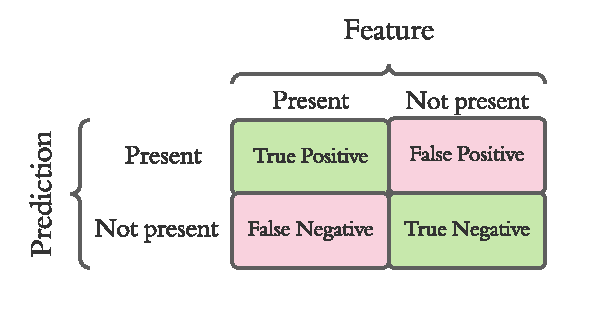
\includegraphics{contextual_review/figures/confusion_matrix.pdf}
    \end{center}
    \caption[Confusion matrix]{
        Confusion matrix showing the meaning of \glsentrylong{tp}, \glsentrylong{tn}, \glsentrylong{fp}, \glsentrylong{fn}.
    }
    \label{fig:confusion_matrix}
\end{figure}
An important step is the fair assessment of algorithms, then, 
    which is achieved through a number of \emph{performance metrics}.
In each supervised \gls{ml}, the machine attempts to learn the structure of $f$ that optimises some internal \gls{of}, 
    e.g. minimising the average distance between predicted and target labels for regression, $\sum\limits_{d \in \mathcal{D}_t} y_d - y^{\prime}_d$.
To assess the resultant model, we introduce a number of \emph{performance metrics}, 
    which aim to measure serveral perspectives of the model's efficacy, by considering the model's predictions with respect to $\mathcal{D}_v$. 
\par 

By definition of the data format, it is relatively straightforward to define metrics for supervised routines:
    the classes assigned to feature vectors, $y_i^{\prime}$, can be quantitatively assessed with respect to their true class, $y_i$. 
For example, in \emph{binary classification}, the output of the model is either correct or incorrect, 
    allowing us to meaningfully assess its average performance. 
Likewise, for numerical targets, the difference $\absval{y_i - y_i^{\prime}}$ between the output, $y_i^{\prime}$, 
    and the target, $y_i$ for each sample cumulatively indicate the strength of the model. 
\par 

There are a large number of quantities and performance metrics against which to judge models' outputs.
In binary classification, we care about whether the model predicts that a given feature is present,
    and whether it predicts features incorrectly. 
For example, the model aims to classify whether or not a dog is present in an image. 
These type of binary predictions have four outcomes, which can be summarised in a \emph{confusion matrix} (\cref{fig:confusion_matrix}), 
    defined as in \cref{table:classification_metrics}.

\begin{table}[H]
    \begin{center}
    \begin{tabular}{lcc}
        & $y$ has feature & $y^{\prime}$ has feature \\
        \hline
        \Glsentryfull{tp} & \tick & \tick \\
        \Glsentryfull{fp} & \cross & \tick \\
        \Glsentryfull{tn} & \cross & \cross \\
        \Glsentryfull{fn} & \tick & \cross\\
    \end{tabular}
    \end{center}
    \caption[Classification metrics]{
        Classification metrics. 
        We define classification outcomes based on whether the considered feature was present and/or predicted. 
    }
    \label{table:classification_metrics}
\end{table}
\par 
    
We can use the concepts of \cref{table:classification_metrics} to define a series of \emph{rates} 
    which characterise the model's predictions. 
    
\begin{description}\label{metrics_description}
    \begin{subequations}
    \item[Accuracy] The overall rate at which the algorithm predicts the correct result. 
    \begin{equation}\label{accuracy_eqn}
        \frac{TP + TN}{TP + TN + FN + FP}
    \end{equation}
    
    \item[Precision] Positive predicitve rate. Of those \emph{predicted to have} the feature of interest, what percentage \emph{actually have} the feature. 
    \begin{equation}\label{precision_eqn}
        \frac{TP}{TP+FP}
    \end{equation}
    
    \item[Sensitivity] True positive rate (also known as \emph{recall}). Of those which \emph{actually have} the feature, what percentage are \emph{predicted to have} the feature.
    \begin{equation}\label{sensitivity_eqn}
        \frac{TP}{TP+FN}
    \end{equation}
    
    \item[Specificity] True negative rate. Of those which  \emph{do not actually have} the feature of interest, how many are \emph{predicted not to} have the feature.
    \begin{equation}\label{specificity_eqn}
        \frac{TN}{TN+FP}
    \end{equation}
    \end{subequations}
\end{description}
    
Each metric has clear advantages, but consider also their drawbacks:
\begin{easylist}
    & Accuracy can be extremely misleading. 
        for example, in a dataset with only 100 instances of the feature of interest,
        a model predicting 9,900 true negatives and 1,100 false negatives will give 99\% accuracy, despite not having found a single positive sample. 
        This is clearly of no use in identifying the minority of cases which are of actual interest. 
    & Sensitivity can be inflated by over-fitting to positive cases. 
        That is, by predicting the feature as present in all cases, all true instances of the feature will be found, however all false instances will be labelled as having the feature, 
        so the model has not helped separate the data.
        The model willl yield a high rate of \gls{tp} but also a high rate of \gls{fp}. 
    & Precision can be high for extremely selective models, i.e. those which are conservative in predicting the presence of the feature.
        By predicting relatively few positive instances, it can ensure that a high proportion of its predictions are correct. 
        The absolute number of instances identified, however, is relatively low, as a proportion of the total number in the dataset. 
    & Specificity, similar to sensitivity, can easily mislead by identifying very few instances as having the target feature. 
        Then, it will correctly predict most non-present instances as false, but will not identify the few instance of interest.  
\end{easylist}

Clearly, the performance metric must be chosen with due consideration for the application;
    e.g. in testing for a medical condition, rather than incorrectly telling a patient they do not have the condition because the 
    model predicted they were feature-negative, it is preferable to incorrectly identify some patients as feature-positive (since they can be retested). 
In this case, high accuracy is crucial, at the expense of precision. 
It is clearly appropriate to blend together the usual metrics, in order to derive performance metrics which balance the priorities of the outcomes.
In general -- including in this thesis -- the most important aspects of a \gls{ml} are precision and sensitivity: 
    a model which performs well with respect to \emph{both} of these is sensitive to the feature, but precise in its predictions. 
A quantity which captures both of these is the $F_{\beta}$-score, 
\begin{equation}\label{eqn:f_beta}
    f_{\beta} = \left( 1 + \beta^2 \right) \frac{
        \textrm{precision} \times \textrm{sensitivity} }{
        \left(\beta^2\times\textrm{precision}\right) + \textrm{sensitivity}},
\end{equation}
where $\beta \in \mathbb{R}$ is the relative weight of importance between sensitivity and precision. 
In particular, considering precision and sensitivity as equally important, i.e. $\beta=1$, 
    we have the $\fs$, 
\begin{equation}
    \label{eqn:f_score_def}
    f_1 = \frac{2 \times \textrm{precision} \times \textrm{sensitivity} }{\textrm{precision} + \textrm{sensitivity}}.
\end{equation}
For examples of how $\fs$ balances these considerations, see \cref{table:f1_example}.
\par

\begin{table}
    \centering
    \begin{tabular}{|ccc|cc|c|}
        \hline
        \Glsentrylong{tp} & \Glsentrylong{fn} & \Glsentrylong{fp} & Precision & Sensitivity & $\fs$  \\
        \hline
        \rule{0pt}{3ex} 500 & 500 & 1000 & 33 & 50 & $ (\frac{2 \times 33 \times 50 }{33 + 50 }) = 37 $ \\
        \rule{0pt}{3ex} 500 & 500 & 500 & 50 & 50 & $( \frac{2 \times 50 \times 50 }{50 + 50 } ) = 50 $ \\
        \rule{0pt}{3ex} 1000 & 0 & 1000 & 50 & 100 & $ (\frac{2 \times 50 \times 100} { 50 + 100 }) = 67 $ \\
        \rule{0pt}{3ex} 1000  & 0 & 0 & 100 & 100 & $ (\frac{2 \times 100 \times 100}{100 + 100}) = 100 $ \\
        \hline
    \end{tabular}
    \caption{$\fs$ examples.}
    \label{table:f1_example}
\end{table}


\subsection{Unsupervised \glsentrylong{ml}}

Contrary to supervised algorithms, unsupervised methods operate on \emph{unlabelled} data, $\mathcal{D}$. 
This is often summarised as finding structure within unstructured data.
Again, we can further compartmentalise methods under this umbrella \cite{geron2019hands}. 
Although we do not utilise these methods in this thesis, we briefly summarise them here for completeness.

\begin{description}
    \item[Clustering] Finding datapoints which are similar to each other, according to some distance metric.
    \begin{easylist}
        && e.g. online retailers grouping together customers with similar preferences, in order to tailor advertising campaigns. 
    \end{easylist}
    \item[Dimensionality reduction] Reducing the feature vector of each sample in a dataset to essential components,
        which may be amalgamations of original features, while retaining structure within the data.
    \begin{easylist}
        && this can be used for visualisation to allow for inspection of complex datasets, 
        e.g. plotting users of a social network as nodes on a 2D map, where distinct social groups
        are kept distant. 
    \end{easylist}
    \item[Association learning] Discover correlations among data. 
    \begin{easylist}
        && For instance, a supermarket may find that purchasers of certain products are likely also to buy others, 
            providing actionable insight 
            e.g. purchases involving bread also include butter in $50\%$ of cases, 
            so positioning these nearby may increase sales by reminding consumers of their compatibility. 
    \end{easylist}
    \item[Semi-supervised learning] Combine elements of supervised and unsupervised algorithms, 
        to achieve a task beyond the remit of either alone. 
        This often means classifying data where only occur a small subset of the total dataset is labelled. 
    \begin{easylist}
        && e.g. in facial recognition, a clustering algorithm finds similarities between individual people in photos, 
            and identifies a single person present across a number of photos, and associates those photos together. 
            It combines this with a small set of photos for which people have been tagged, 
                locates the same person and automatically tags them in the wider set of photos. 
    \end{easylist}
\end{description}
\par 

\subsection{\Glsentrylong{rl}}
A third category of \gls{ml} algorithms are \glsentryfull{rl}. 
These are methods where an \emph{agent} interacts with some environment, 
    and refines a \emph{policy} for reacting to different stimuli. 
As such, the agent can, in principle, deal with a wide array of situations. 
These methods underly technologies such as self-driving cars, 
    which inspect their surroundings through \emph{sensors};
    compute an \emph{action} according to the policy; 
    implement that action through \emph{actuators}.
Following an action, the agent senses whether that action was beneficial or detrimental, 
    and receives a \emph{reward} or \emph{punishment} accordingly. 
Highly rewarded actions are likely to be repeated in future, allowing the agent to learn what response is 
    appropriate to situational parameters, 
    e.g. a self-driving car braking at a red light is rewarded, 
    while braking at a green light is punished. 
\par 
The concept of a machine's \emph{agency} is an ongoing discussion in the \gls{ml} community \cite{franklin1996agent, wooldridge2009introduction}, 
    and is important in this thesis also, when we define our model learning protocol as an agent, 
    since it designs models by interacting with the envinroment of the target quantum systems. 
We will revisit the concept in \cref{sec:agency}.

\section{Quantum \glsentrylong{ml}}
\begin{figure}
    \begin{center}
        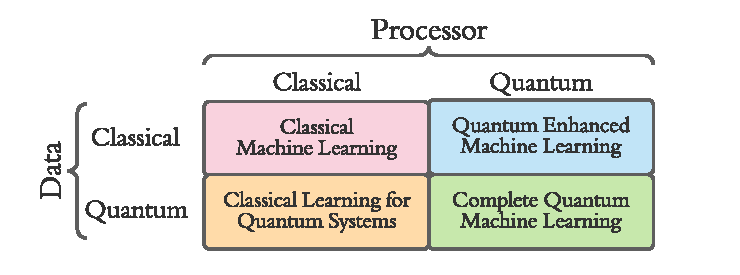
\includegraphics{contextual_review/figures/qml_types.pdf}
    \end{center}
    \caption[Types of \glsentrylong{qml}]{Types of \glsentrylong{qml}.}
    \label{fig:qml_types}
\end{figure}
A growing domain is the development of \gls{ml} algorithms which run on quantum hardware, 
    or exploit data from quantum systems; generally referred to as \gls{qml} \cite{biamonte2017quantum, adcock2015advances}. 
There are a number of metehodologies which are referred to as \gls{qml};
    for clarity, we define the main branches here, as shown in \cref{fig:qml_types}. 

\begin{description}\label{description:qml}
    \item[Classical machine learning] 
        refers to standard \gls{ml} as described in \cref{sec:classical_ml}, i.e. where the processors are \glspl{cpu} or \glspl{gpu}, 
            and the applications are not of specific interest to problems in the quantum domain. 
        Recently, this branch has encompassed quantum \emph{inspired} \gls{ml}, which still target classical problems, 
            but use subroutines which were orginally found in the context of \gls{qml} \cite{tang2019quantum}.

    \item[Quantum enhanced machine learning] 
        A quantum co-processor is leveraged on classical data for some provable speedup,
        i.e. data that could otherwise be processed purely classically, is encoded, loaded onto and processed by quantum hardware.
        The quantum counterparts of classical \gls{ml} algorithms aim to solve the same problems, 
            e.g. as \glspl{nn} \cite{schuld2014quest, cao2017quantum} and principle component analysis \cite{lloyd2014quantum}. 

    \item[Classical learning for quantum systems] 
        Classical processors are employed to extract insight on problems arising from quantum systems, 
            e.g. data is taken from a quantum system and analysed via purely classical methods.
            For instance, methods which aim to represent quantum states efficiently by leveraging 
            \glspl{nn} \cite{carleo2017solving, torlai2018neural}. 

    \item[Complete quantum machine learning] 
        Data of a quantum nature is processed -- at least partially -- by quantum processors. 
        The most common technique here is \gls{vqe}, which simulates quanutm systems on \glspl{qc}, 
        in order to retrieve quantum systems' ground states \cite{peruzzo2014variational}.
        The algorithm relies on a classical optimisation routine, but was devised explicitly for implementation on quantum hardware. 
\end{description}
\par 

The algorithms described in \cref{part:algorithms} and the applications in \crefrange{part:experimental_study}{part:theoretical_study} 
    can be described as classical learning for quantum systems. 
This is because the data upon which the applications are built represent quantum systems, 
    but are processed through classical \gls{ml} algorithms in order to derive insight about those systems.
We caveat that it is feasible, and indeed the long term intention of such algorithms, 
    to run in conjunction with a quantum co-processor, which would represent and evolve quantum systems, 
    but all processing presented here are through strictly classical architecture.

\section{\Glsentrylongpl{ga}}\label{sec:genetic_algorithms}
In later chapters we will use a class of optimisation techniques known as \emph{evolutionary algorithms} \cite{back1996evolutionary, de2020evolutionary}.
In particular, \emph{\glsentryfullpl{ga}} are central to our primary applications, 
    specifically in \cref{chapter:ga}.
Here we describe \glspl{ga} in general terms for reference in later chapters. 
\par 
\glspl{ga} work by assuming a given problem can be optimised, if not solved, by a single candidate 
    among a fixed, closed space of candidates, called the population, $\population$. 
A number of candidates are sampled at random from $\population$ into a single \emph{generation}, 
    and evaluated through some \glsentryfull{of}, which assesses the fitness of the candidates at solving the problem of interest. 
Candidates from the generation are then mixed together to produce the next generation's candidates: 
    this \emph{crossover} process aims to combine only relatively strong candidates, such that the average 
    candidates' fitness improve at each successive generation, 
    mimicing the biological mechanism whereby the genetic makeup of offspring is an even mixture of both parents
    through the philosophy of \emph{survival of the fittest}. 
The selection of strong candidates as parents for future generations is therefore imperative; 
    in general parents are chosen according to their fitness as determined by the \gls{of}. 
Buidling on this biological motivation, much of the power of \glspl{ga} comes from the concept of \emph{mutation}: 
    while offspring retain most of the genetic expressions of their parents, some elements are mutated at random.
Mutation is crucial in avoiding local optima of the \gls{of} landscape
    by maintaining diversity in the examined subspace of the population.
\par 

\glspl{ga} are not defined either as supervised or unspervised methods;
    this designation depends on the \gls{of}. 
If candidates are evaluated with respect to labelled data, we can consider that \gls{ga} supervised, 
    otherwise unsupervised. 
Pseudocode for a generic \gls{ga} is given in \cref{alg:ga},
    but we can also informally define the procedure as follows. 
Given access to the population, $\population$, 

\begin{easylist}[enumerate]\label{mark:informal_ga}
    \ListProperties(Numbers2=l, Numbers3=r)
    & Sample $N_m$ candidates from the population at random
    && call this group of candidates the first generation, $\mu$. 
    & \label{ga:loop} Evaluate each candidate $\gamma_j \in \mu$
    && each $\gamma_j$ is assigned a fitness, $g_j$;
    && the fitness is computed through an objective function acting on the candidate, i.e. $g_j = g(\gamma_j)$. 
    & Map the fitnesses of each candidate, $\{g_j\}$, to selection probabilities for each candidate, $\{s_j\}$
    && e.g. by normalising the fitnesses, or by removing some poorly-performing candidates and then normalising. 
    & Generate the next generation of candidates
    && Reset $\mu = \{ \}$;
    && \label{ga:select} Select pairs of parents, $\left\{\gamma_{p_1}, \gamma_{p_2}\right\}$, from $\mu$
    &&& Each candidate's probability of being chosen is given by their $s_j$.
    && Cross over $\left\{\gamma_{p_1}, \gamma_{p_2}\right\}$ to produce children candidates, $\left\{\gamma_{c_1}, \gamma_{c_2}\right\}$
    &&& mutate $\gamma_{c_1}, \gamma_{c_2}$ according to some random probabilistic process;
    &&& keep $\gamma_{c_i}$ only if it is not already in $\mu$, to ensure $N_m$ unique candidates are tested at each generation.
    && until $|\mu| = N_m$, iterate to step (\ref{ga:select}.
    & Until the $N_g^{th}$ generation is reached, iterate to step \ref{ga:loop};
    & The strongest candidate on the final generation is deemed the solution to the posed problem. 
\end{easylist}


\begin{algorithm}
    \caption{Genetic algorithm}
    \label{alg:ga}
    \DontPrintSemicolon
    \KwIn{ $\population$ \tcp*[1]{Population of candidate models}}
    \KwIn{ $g()$ \tcp*[1]{objective funtion}}
    \KwIn{ $\ttt{map\_g\_to\_s}()$ \tcp*[1]{function to map fitness to selection probability}}
    \KwIn{ $\ttt{select\_parents}()$ \tcp*[1]{function to select parents among generation}}
    \KwIn{ $\ttt{crossover}()$ \tcp*[1]{function to cross over two parents to produce offspring}}
    \KwIn{ $N_g$ \tcp*[1]{number of generations}}
    \KwIn{ $N_m$ \tcp*[1]{number of candidates per generation}}\;

    \KwOut{$\gamma^{\prime}$ \tcp*[1]{strongest candidate}}\;
    
    $\mu \gets \ttt{sample} \left( \population, N_m\right)$\; 

    \For{$i \in 1, ..., N_g$}{
        \For{$\gamma_j \in \mu$ }{
            $g_j \gets g(\gamma_j) $ \tcp*[1]{assess fitness of candidate}
        }

        $\{ s_j \}  \gets \ttt{ map\_g\_to\_s}(\{g_j \})$ \tcp*[1]{map fitnesses to normalised selection probability}
        $\mu_c = \argmax\limits_{s_j} \{ \gamma_j \}$ \tcp*[1]{record champion of this generation}\;

        $\mu \gets \{ \}$ \tcp*[1]{empty set for next generation}

        \While{$| \mu | < N_m$}{
            $p_1, p_2 \gets \ttt{select\_parents}(\{s_j\})$ \tcp*[1]{choose parents based on candidates' $s_j$}
            $c_1, c_2 \gets \ttt{crossover}(p_1,p_2)$ \tcp*[1]{generate offspring candidates based on parents}

            \For{$c \in \{c_1, c_2\}$ }{
                \If{$c \notin \mu$}{
                    $\mu \gets \mu \cup \{ c\}$ \tcp*[1]{keep if child is new} 
                }
            }
        }
    }

    $\gamma^{\prime} \gets \argmax\limits_{s_j}\{ \gamma_j \in \mu \}$ \tcp*[1]{strongest candidate on final generation}\;

    return $\gamma^{\prime}$

\end{algorithm}


\par 

Candidates are manifested as \emph{\glspl{chromosome}}, i.e. strings of fixed length, 
    whose entries, called  \emph{\glspl{gene}}, each represent some element of the system.
In general, \glspl{gene} can have continuous values, although usually, and for all purposes in this thesis, 
    genes are binary, capturing simply whether or not the \gls{gene}'s corresponding feature is present 
    in the \gls{chromosome}. 

\subsection{Example: knapsack problem}\label{sec:knapsack}
\begin{figure}
    \begin{center}
        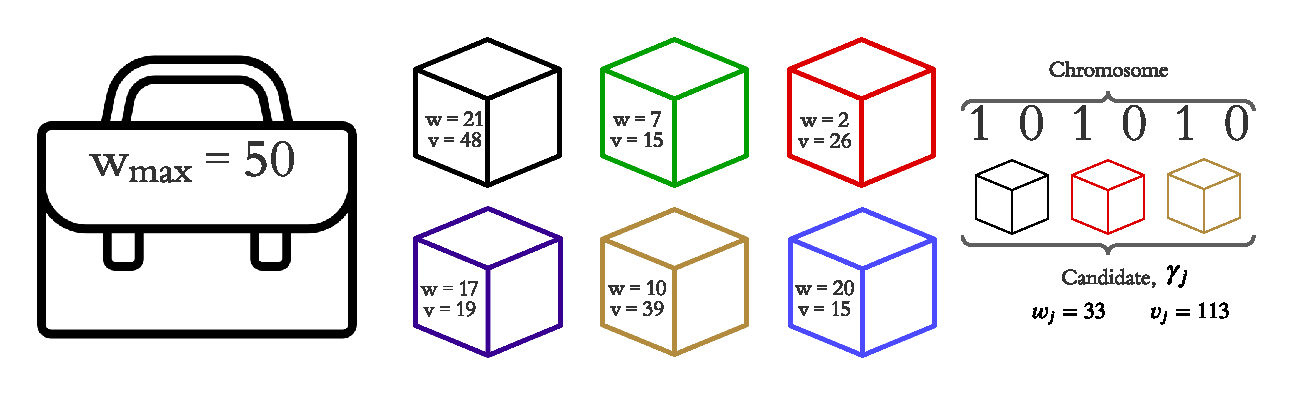
\includegraphics[width=\textwidth]{theoretical_study/figures/knapsack_schematic.pdf}
    \end{center}
    \caption[Knapsack problem]{
        Depiction of the knapsack problem.
        \textbf{Left}, A knapsack which can hold any number of objects but is constrained by the total weight it can support, 
        $w_{max} = 50$. 
        \textbf{Centre}, A set of objects are available, each with associated weight, $w$, and value $v$. 
        The objective is to find the subset of objects which maximise the total value, 
        while not exceeding the capacity of the knapsack. 
        \textbf{Right}, An example chromosome, i.e. candidate $\gamma_j$, where the bits of the chromosome indicate 
            whether the corresponding object is included, allowing for calculation of the total weight and value of 
            the candidate, $w_{j}, v_{j}$. 
    }

\end{figure}
One commonly referenced combinatorial optimisation problem is the \emph{knacksack problem}: 
    given a set of objects, where each object has a defined mass and also a defined value, 
    determine the set of objects to pack in a knapsack which can support a limited weight, 
    such that the value of the packed objects is maximised. 
Say there are $n$ objects, 
    we can write the vector containing the values of those objects as $\vec{v}$, 
    and the vector of their weights as $\vec{w}$. 
We can then represent configurations of object sets as candidate vectors $\vec{\gamma}_j$, 
    whose genes are binary, and simply indicate whether or not the associated object is included in the set. 
For example, with $n=6$,
\begin{equation}
    \gamma_j = \ttt{100001} \Longrightarrow \vec{\gamma}_j = \irow{1 & 0 & 0 & 0 & 0 & 1},
\end{equation} 
indicates a set of objects consisting only of those indexed first and last, with none of the intermediate objects included. 

\par
The fitness of any candidate is then given by the total value of that configuration of objects, $v_j = \vec{v} \cdot \vec{\gamma}_j$, 
    but candidates are only admitted\footnotemark \ if the weight of the corresponding set of objects 
    is less than the capacity of the knapsack, i.e. $\vec{w}_j \cdot \vec{\gamma}_j \leq w_{max}$. 
\footnotetext{
    Note there are alternative strategies to dealing with candidates who violate the weight condition, 
    such as to impose a penalty within the \gls{of}, but for our purposes let us assume we simply disregard violators. 
}
\par 

For example where each individual object has value $<50$ and weight $<25$ and $w_{max} = 50$, 
recalling $\gamma_j = \ttt{100001}$, say, 
\begin{subequations}
    \begin{equation}
        \vec{ v } = \irow{ 48 & 15 & 26 & 19 & 39 & 15 } \Longrightarrow v_j = \vec{\gamma}_j \cdot \vec{v} = 48 + 15 = 63;
    \end{equation}
    \begin{equation}
        \vec{ w } = \irow{ 21 & 7 & 2 & 17 & 10 & 20 } \Longrightarrow w_j = \vec{\gamma}_j \cdot \vec{w} = 21 + 20 = 41.
    \end{equation}
\end{subequations}
We can hence assess the fitness of $\gamma_j$ as $63$ and deem it a valid candidate since it does not exceed the weight threshold.
We can likewise compute the total weight and value of a series of randomly generated candidates, 
    and deem them valid or not. 
\cref{table:knapsack_candidates} shows a set of 12 randomly generated candidates, 
    of which ten are valid.

\begin{table}[H]
    \begin{center}
        \begin{tabular}{llrrl}
\hline
              &        &                                    Value &                                   Weight &                                    Valid \\
Name & Candidate &                                          &                                          &                                          \\
\midrule
$\gamma_{1}$ & 110011 &                                      117 &                                       58 &                                       No \\
$\gamma_{2}$ & 101010 &                                      113 &                                       33 &                                      Yes \\
$\gamma_{3}$ & 011110 &                                       99 &                                       36 &                                      Yes \\
$\gamma_{4}$ & 011011 &                                       95 &                                       39 &                                      Yes \\
$\gamma_{5}$ & 111000 &                                       89 &                                       30 &                                      Yes \\
$\gamma_{6}$ & 010111 &                                       88 &                                       54 &                                       No \\
$\gamma_{7}$ & 100010 &                                       87 &                                       31 &                                      Yes \\
$\gamma_{8}$ & 110001 &                                       78 &                                       48 &                                      Yes \\
$\gamma_{9}$ & 011101 &                                       75 &                                       46 &                                      Yes \\
$\gamma_{10}$ & 110000 &                                       63 &                                       28 &                                      Yes \\
$\gamma_{11}$ & 000011 &                                       54 &                                       30 &                                      Yes \\
$\gamma_{12}$ & 000101 &                                       34 &                                       37 &                                      Yes \\
\hline
\end{tabular}

        \caption[Candidate solutions to knapsack problem]{
            Candidate solutions to the knapsack problem for randomly generated chromosomes. 
        }
        \label{table:knapsack_candidates}
    \end{center}
\end{table}

The strongest (valid) candidates from \cref{table:knapsack_candidates} are \ttt{101010}, \ttt{011110}. 
By spawning from these candidates through a one-point crossover at the midpoint\footnotemark, 
    we get $\gamma_{c_1} = \ttt{101110}, \gamma_{c_2} = \ttt{011010}$, 
    from which we can see $v_{c_1} = 132, w_{c_1} = 50$, i.e. by combining two strong candidates we produce 
    the strongest-yet-seen valid candidate. 
\footnotetext{One-point crossovers are detailed in \cref{sec:reproduction} with this example shown in \cref{fig:gen_alg_reproduction}.}
\par 

By repeating this procedure, it is expected to uncover candidates which optimise $v_j$ while maintining $w_j \leq w_{max}$, 
    or at least to produce near-optimal solutions, using far less time/resources than brute-force evaluation of all candidates, 
    which is usually sufficient. 
For instance, with $n=100$ objects to consider, there are $2^{100} \approx 10^{30}$ candidates to consider; 
    the most powerful supercomputers in the world currently claim on the order of Exa-FLOPs, 
    i.e. $10^{18}$ operations per second, of which say $\mathcal{O}(1000)$ operations are required to test each candidate, 
    meaning $10^{15}$ candidates can be checked per second in a generous example. 
This would still require $10^{12}$ seconds to solve absolutely, 
    so it is reasonable in cases like this to accept 
    \emph{approximately optimal} solutions\footnote{
        Simply put: in machine learning, \emph{good enough} is good enough.
        We will adopt this philosophy for the remainder of this thesis and life. 
    }. 


\subsection{Selection mechanism}
\begin{figure}
    \begin{center}
        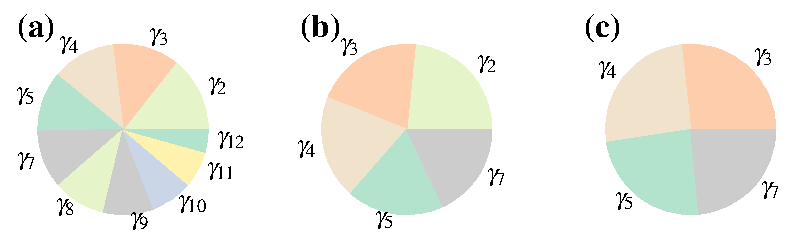
\includegraphics{theoretical_study/figures/knapsack_roulette.pdf}
    \end{center}
    \caption[Roulette wheels for selection]{
        Roulette wheels showing selection probability $s_i$ for corresponding candidates $\gamma_i$. 
        Colours here only distinguish candidates, they do not encode any information. 
        \textbf{b}, The set of potential parents is truncated to include only the strongest five candidates. 
        \textbf{a}, All valid candidates are assigned selection probability based on their value in \cref{table:knapsack_candidates}. 
        \textbf{c}, After one parent ($\gamma_2$) has been chosen, it is removed from the roulette wheel and the remaining
         candidates' probabilities are renormalised for the selection of the second parent. 
    }
    \label{fig:knapsack_roulette}
\end{figure}

A key subroutine of every \gls{ga} is the mechanism through which it nominates candidates from generation $\mu$ 
as parents to offsping candidates in $\mu+1$ \cite{luke11}. 
All mechanisms have in common that they act on a set of candidates from the previous generation, 
    where each candidate, $\gamma_j$, has been evaluated and has fitness value, $g_j$. 
Among the viable schemes for selecting individual parents from the set of candidates, $\mu$  are
\begin{easylist}[itemize]
    & Rank selection: candidates are selected with probabilty proportional to their ranking relative to 
        the fitness of contemporary candidates in the same generation;
    & Tournament selection: a subset of $k$ candidates are chosen at random from $\mu$, 
        of which the candidate with the highest fitness is taken as the parent;
    & Stochastic universal sampling: candidates are sampled proportional to their fitness, 
        but the sampling algorithm is biased to ensure high-fitness candidates are chosen at least once 
        within the generation. 
\end{easylist}

We will only detail the mechanism used in later applications within this thesis: 
    fitness proportional selection, known as \emph{roulette selection} \cite{luke11}. 
This is a straightforward strategy where we directly map candidates' fitness, $g_i$ to a selection probability, $s_i$,
    simply by normalising $\{g_i\}$, 
    allowing us to visualise a roulette wheel of uneven wedges, each of which correspond to a candidate. 
Then we need only conceptually spin the roulette wheel to select the first parent, $\gamma_{p_1}$. 
We then remove $\gamma_{p_1}$ from the set of potential parents, renormalise the remaining $\{s_i\}$, 
    and spin the wheel again to choose the second parent, $\gamma_{p_2}$. 
The roulette selection is shown in \cref{fig:knapsack_roulette}.
\par 

Practically, we repeat the process outlined until the next generation is filled, 
    usually we have $|\mu| = N_m$, and desire that every generation should contain the same 
    $N_m$ candidates, so we repeat the roulette selection $\nicefrac{N_m}{2}$ times per generation, 
    since every pair of parents yield two offspring.
It is important that meaningful differences in fitness are reflected by the selection probability, 
    which is difficult to ensure for large $N_m$, e.g. with ten models, the strongest candidate is only 
    a marginally more probable parent than the worst -- this effect is amplified for larger $N_m$. 
We therefore wish to reduce the set of potential parents to ensure high quality offspring:
    we truncate $\mu$ and retain only the highest-fitness $\frac{N_m}{2}$ models as selectable parents. 
\par 

\subsection{Reproduction}
\label{sec:reproduction}
\begin{figure}
    \begin{center}
        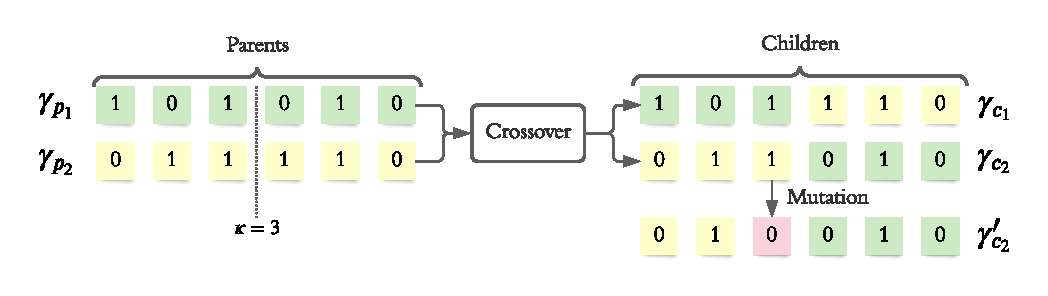
\includegraphics{theoretical_study/figures/chromosomes.pdf}
    \end{center}
    \caption[Crossover and mutation of chromosomes]{
        Crossover and mutation of chromosomes.
        Two parents, $\left\{\gamma_{p_1}, \gamma_{p_2}\right\}$, are nominated from the process in \cref{fig:knapsack_roulette}. 
        They are then crossed-over via a one-point crossover with crossing point $\kappa=3$, 
        resulting in children candidates $\left\{\gamma_{c_1}, \gamma_{c_2}\right\}$. 
        One child chromosome is mutated to yield a new candidate, $\gamma_{c_2}^{\prime}$. 
        The candidates added to the next generation are then $\{ \gamma_{c_1}, \gamma_{c_2}^{\prime} \}$.
    }
    \label{fig:gen_alg_reproduction}
\end{figure}

When a pair of parents have been nominated by the selection mechanism above, 
    it remains to use those parents to \emph{reproduce}, 
    i.e. to produce offspring which should inherit and improve upon the properties of their parents. 
Here we use a \emph{one point crossover}, whereby the two parent chromosomes are mixed together 
    to form two offspring, about a single point, $\kappa$: 
    for candidates of $n$ genes, 
    the first $\kappa$ genes of $\gamma_{p_1}$ are conjoined with the latter $n - \kappa$ genes of $\gamma_{p_2}$. 
Often $\kappa$ is restricted to the midpoint of the chromosomes, although in general we need not impose this: 
    we will instead consider $\kappa \in \left( \frac{n}{4}, \frac{3n}{4} \right)$, 
    e.g. with $n=12$, $\kappa \in (3, 9)$. 
The one-point crossover is shown for $n=6$ with $\kappa=3$ in \cref{fig:gen_alg_reproduction}, 
    recalling the chromosome structure from \cref{sec:knapsack}.
\par 
By allowing $\kappa$ other than the midpoint, we drastically increase the number of combinations of parents available for reproduction. 
Finally, then, parent selection is done by constructing a database of pairs of potentital parents with all available crossover points, 
    with selection probability given by the product of their individual fitnesses. 
This is conceptually equivalent to selection via roulette wheel as above. 
Recalling the fitnesses (values) of \cref{table:knapsack_candidates}, we generate the parent selection database:

\begin{table}[H]
    \begin{center}
        \begin{tabular}{cccc}
            Parent 1 & Parent 2 & $\kappa$ & $s_{ij}$ \\
            \hline 
            $\gamma_2$ & $\gamma_3$ & 2 & $11,187 \ (=113 \times 99 )$ \\
            $\gamma_2$ & $\gamma_3$ & 3 & $11,187$ \\
            $\gamma_2$ & $\gamma_3$ & 4 & $11,187$ \\

            $\gamma_2$ & $\gamma_4$ & 2 & $10,735 \ (=113 \times 95)$ \\
            $\gamma_2$ & $\gamma_4$ & 3 & $10,735$ \\
            $\gamma_2$ & $\gamma_4$ & 4 & $10,735$ \\

             & & \vdots & \\

            $\gamma_5$ & $\gamma_7$ & 2 & $7,743 \ (=89 \times 87)$ \\
            $\gamma_5$ & $\gamma_7$ & 3 & $7,743$ \\
            $\gamma_5$ & $\gamma_7$ & 4 & $7,743$ \\

        \end{tabular}
    \end{center}
    \caption[Genetic algorithm parent selection database]{
        Example of parent selection database. 
        Pairs of parents are selected together, with the (unnormalised) selection probability, $s_{ij}$, 
        given by the product of the individual candidates' fitnesses. 
        Pairs of parents are repeated in the database for differing $\kappa$, 
            and all $\kappa$ are equally likely. 
    }
    \label{table:selection_database}
\end{table}
    

The \gls{ga} maintains diversity in the subspace of $\population$ it studies, 
    by \emph{mutating} some of the newly proposed offspring candidates. 
Again, there are a multitude of approaches for this step \cite{schmitt2001theory}, 
    but for brevity we only describe those used in this thesis.
For each proposed child candidate, $\gamma_{c}$, we probabilistically mutate each gene with some mutation rate $r_m$:
    if a mutation occurs, the child is replaced by $\gamma_c^{\prime}$. 
That is, $\gamma_c^{\prime}$  is added to the next generation, and $\gamma_c$ is discarded. 
$r_m$ is a \emph{hyperparameter} of the \gls{ga}:
    the performance of the algorithm can be optimised by finding the best $r_m$ 
    for a given problem. 

\subsection{Candidate evaluation}
\label{sec:candidate_evaluation}
Within every generation of the \gls{ga}, each candidate must be evaluated, 
    so that the relative strength of candidates can be exploited in constructing 
    candidates for the next generation.
In the example of the knapsack problem used above, candidates were evaluated by the value of their contents, 
    but also by whether they would fit in the knapsack. 
Idenitfiyng the appropriate method by which to evaluate candidates is arguably the most important aspect of designing a \gls{ga}:
    while the choice of hyperperameters ($N_g, N_m, r_m$) dictate the efficacy of the search, 
    the lack of an effective metric by which to distinguish candidates would render the procedure pointless.
Considerations are hence usually built into the \glsentryfull{of};
    \glspl{ga} implementations later in this thesis therefore demand we design \glspl{of} 
    with respect to the individual application. 
\par 






\part{Algorithms}\label{part:algorithms}
    \chapter*{Overivew and contribution}
        \addcontentsline{toc}{chapter}{Overview and contributions}

This Part details the algorithms which form the basis for the research conducted in this thesis. 
The corresponding software is a primary outcome of this thesis \cite{flynn2021Quantum, flynn2021QMLA, qmla_docs}.

\par 
\vspace{1cm}

\Cref{chapter:qhl} introduces \gls{qhl}, an algorithm for the optimisation of \gls{hamiltonian} parameters
    when the form of the model describing a system of interest is known. 
    This is not presented as new work, but rather as a bedrock for later discussions. 
    The analysis and figures presented in this chapter are unique to this thesis but do not necessarily offer novel insights. 
\par 
\vspace{1cm}
\Cref{chapter:qmla} builds upon \gls{qhl} by posing the question: 
    without assuming access to the model describing the target system, can we combine model training algorithms, 
    in particular \gls{qhl}, with model recovery methodologies, to learn the \gls{hamiltonian} model 
    governing the system, and hence uncover the physics of quantum systems. 
    This motivation leads to the \acrfull{qmla}: 
    a machine learning framework for reverse engineering models of quantum systems from their data.
    This protocol was initially devised by Dr. Raffaele Santagati, 
    and developed toegether with myself and Drs. Andreas Gentile, Stefano Paesani, Nathan Wiebe and Chris Granade. 
    The protocol has been published in \cite{gentile2020learning}, 
    and applied to numerous case studies, which are described in later Parts. 
\par
\vspace{1cm}

\Cref{chapter:sw} describes the implementation of \gls{qmla} through an open source software package. 
I was the principal designer and programmer of the codebase described, which constitutes a large portion of the output of my research. 
The results presented in \cref{part:theoretical_study}, \cref{part:experimental_study} are all achieved through this framework. 

    \chapter{Quantum Hamiltonian Learning}\label{chapter:qhl}
        First suggested in \cite{Granade:2012kj} and since developed \cite{wiebe2014qhlpra, Wiebe:2014qhl} 
    and implemented \cite{wang2017experimental,gentile2020learning}, 
\gls{qhl} is a machine learning algorithm for the optimisation of a given Hamiltonian parameterisation 
    against a quantum system whose model is known apriori. 
Given a target quantum system $Q$ known to be described by some Hamiltonian $\hat{H}(\vec{\alpha})$, 
    \gls{qhl} optimises $\vec{\alpha}$.
This is achieved by interrogating $Q$ and comparing its outputs against proposals $\vec{\alpha}_p$. 
In particular, an experiment is designed, consisting of an input state, $\ket{\psi}$, and an evolution time, $t$.
This experiment is performed on $Q$, whereupon its measurement yields the datum $d \in \{0, 1\}$, 
    according to the expectation value $\left| \bra{\psi} e^{-i \ho t} \ket{\psi} \right|^2$. 
Then on a trusted (quantum) simulator, proposed parameters $\vec{\alpha}_p$ are encoded to the 
    known Hamiltonian, and the same probe state is evolved for the chosen $t$ and projected on to $d$, 
    i.e. $\left| \bra{d} e^{-i \hat{H}(\vec{\alpha}_p) t } \ket{\psi} \right|^2 $ is computed.
The task for \gls{qhl} is then to find $\vec{\alpha}^{\prime}$ for which this quantity 
    is close to 1 for all values of $(\ket{\psi}, t)$, 
    i.e. the parameters input to the simulation produce dynamics consistenst with those measured from $Q$.
\par 

The procedure is as follows. 
A \emph{prior} probability distribution $\pra$ of dimension $\left| \al \right|$ 
    is initialised to represent the constituent parameters of $\al$. 
$\pra$ is typically a multivariate normal (Gaussian) distribution; 
    it is therefore necessary to pre-suppose some mean and width for each parameter in $\al$. 
This imposes prior knowledge on the algorithm whereby the programmer must decide the range in 
    which parameters are \emph{likely} to fit:
    although \gls{qhl} is generally robust and capable of finding parameters outside of this prior,
    the prior must at least capture the order of magnitude of the target parameters. 
An example of imposing such domain-specific prior knowledge is, 
    when choosing the prior for a model representing an $e^-$ spin in a \gls{nv} centre,
    to select $GHz$ parameters for the electron spin's rotation terms, and $MHz$ terms 
    for the spin's coupling to nuclei, as proposed in literature. 
It is important to understand, then, that \gls{qhl} removes the prior knowledge 
    of precisely the parameter representing an interaction in $Q$, but does rely on a ball-park estimate thereof from which to start. 
\par 

In short, \gls{qhl} samples parameter vectors $\al_p$ from $\pra$, 
    simulates experiments by computing the \emph{likelihood} $\left| \bra{d} e^{-i \hat{H}(\al_p)t} \ket{\psi} \right|^2$
    for experiments ($\ket{\psi}, t)$ designed by a \gls{qhl} heuristic subroutine, 
    and iteratively improves the probability distribution of the parameterisation $\pra$ 
    through standard \emph{Bayesian inference}. 
A given set of $(\ket{\psi}, t)$ is called an experiment, since it corresponds to preparing, evolving and measuring $Q$ 
once\footnote{experimentally, this may involve repeating a measurement many times to determine a majority result and to mitigate noise}. 
\gls{qhl} iterates for $\Ne$ experiments. 
The parameter vectors sampled are called \emph{particles}: there are $\Np$ particles used per experiment. 
Each particle used incurs one further calculation of the likelihood function -- 
    this calculation, on a classical computer, is exponential in the number of qubits of the model under consideration
    (because each unitary evolution relies on the exponential of the $2^n \times 2^n$ Hamiltonian matrix of $n$ qubits). 
Likewise, each additional experiment incurs the cost of calculation of $\Np$ particles, 
    so the total cost of running \gls{qhl} for a single model is $\propto \Ne \Np$.
It is therefore preferable to use as few particles and experiments as possible, 
    though it is important to include sufficient resources that the parameter estimates have the opportunity to converge. 
Access to a fully operational, trusted quantum simulator admits an exponential 
    speedup by simulating the unitary evolution instead of computing the matrix exponential classically.
\par 

\section{Bayes Rule}
Bayes' rule is used to update a probability distribution describing hypotheses, $\Pr(\textrm{hypothesis})$, when presented with new information (data).
That is, the probabilty that a hypothesis is true is replaced
    by the initial probability that is was true, $\Pr(\textrm{hypothesis})$, multiplied by 
    the \gls{likelihood} that the new data would be observed were that hypothesis true, 
    $\Pr(\textrm{data} | \textrm{hypothesis})$, 
    normalsied by the probability of observing that data in the first place, $\Pr(\textrm{data})$. 
It is stated as
    \begin{equation}\label{eqn:bayes_rule}
        \Pr( \textrm{hypothesis} | \textrm{data} ) = 
        \frac{ \Pr( \textrm{data} | \textrm{hypothesis} ) \times \Pr( \textrm{hypothesis} )}{ \Pr(\textrm{data})}.
    \end{equation}
\par 
We wish to represent our knowledge of Hamiltonian parameters with a distribution, $\Pr(\al)$:
    in this case hypotheses $\al$ attempt to describe data, $\expdata$, measured from the target quantum system,  
    from a set of experiments $\expset$, so we can rewrite Bayes' rule as 
\begin{equation}\label{eqn:qhl_bayes_rule}
    \Pr(\vec{\alpha} | \expdata; \expset) = \frac{\Pr(\expdata| \vec{\alpha}; \expset) \ \Pr(\vec{\alpha})}{\Pr(\expdata|\expset)}.
\end{equation}

We can then discretise \cref{eqn:qhl_bayes_rule} to the level of single particles (individual vectors in the parameter space), sampled from $\Pr(\al)$:
\begin{equation}\label{eqn:particle_bayes_rule}
    \Pr(\al_p | d; e) = \frac{ \Pr(d | \ \al_p; \ e ) \ \Pr(\al_p) } {\Pr(d | e)}
\end{equation}

where 
\begin{easylist}[itemize]
    & $e$ are the experimental controls of a single experiment, e.g. evolution time and input probe state;
    & $d$ is the datum, i.e. the binary outcome of measuring $Q$ under conditions $e$;  
    & $\al_p$ is the \emph{hypothesis}, i.e. a single parameter vector, called a particle, sampled from $\Pr(\al)$;
    & $\Pr(\al_p | d; e)$ is the \emph{updated} probability of this particle following the experiment $e$, 
        i.e. accounting for new datum $d$, the probability that $\al=\al_0$;
    & $\Pr(d |\al_p ; e)$ is the likelihood function, 
        i.e how likely it is to have measured the datum $d$ from the system assuming $\al_p$ are the true parameters
        and the experiment $e$ was performed; 
    & $\Pr(\al_p)$ is the probability that $\al_p=\al_0$ according to the prior distribution $\Pr(\al)$, 
        which we can immediately access; 
    & $\Pr(d|e)$ is a normalisation factor, the chance of observing $d$ from experiment $e$ irrespective of the underlying hypothesis.
\end{easylist}

In order to compute the updated probability for a given particle, then, all that is required is a value for the likelihood function.
This is equivalent to the expectation value of projecting $\ket{\psi}$ onto $d$, after evolving $\hat{H}(\al_p)$ for $t$, i.e. 
\begin{equation}
    \label{eqn:likelihood}
    \Pr(d | \al; e) = \left| \bra{d} e^{-i \hat{H}(\al_p)t} \ket{\psi} \right|^2,   
\end{equation}
    which can be simulated clasically or using a quantum simulator (see \cref{sec:likelihood}). 
It is necessary first to know the datum $d$ (either 0 or 1) which was projected by $Q$ under real experimental conditions. 
Therefore we first perform the experiment $e$ on $Q$ 
    (preparing the state $\ket{\psi}$ evolving for $t$ and projecting again onto $\bra{\psi}$)
    to retrieve the datum $d$. 
$d$ is then used for the calculation of the likelihood for each particle sampled from $Pr({\al})$. 
Each particle's probability can be updated by \cref{eqn:particle_bayes_rule}, 
    allowing us to redraw the entire probability distribution -- i.e. we compute a \emph{posterior} probability distribution
    by performing this routine on $\Np$ particles. 


\section{Sequential Monte Carlo}\label{sec:smc}
\begin{figure}
    \setcounter{subfigure}{0}

    \centering
    \subfloat{
        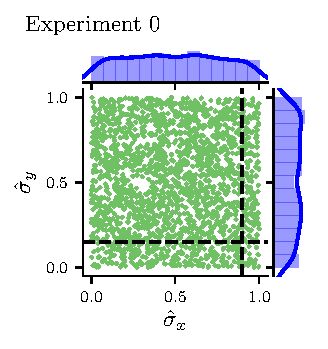
\includegraphics{algorithms/figures/smc_demo/epoch_0.pdf}
    }
    \subfloat{
        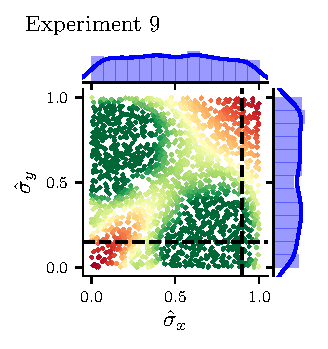
\includegraphics{algorithms/figures/smc_demo/epoch_9.pdf}
    }
    \subfloat{
        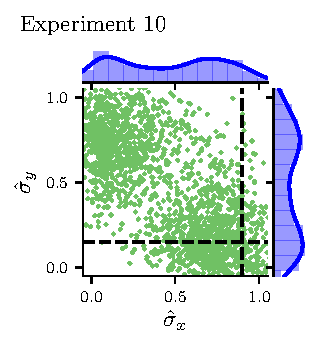
\includegraphics{algorithms/figures/smc_demo/epoch_10.pdf}
    }
    % \hspace{0mm}
    
    \subfloat{
        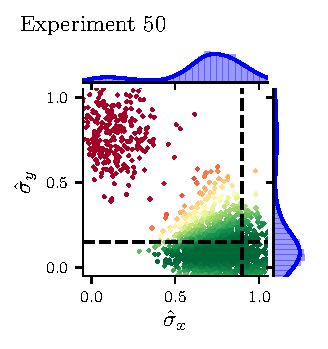
\includegraphics{algorithms/figures/smc_demo/epoch_50.pdf}
    }
    \subfloat{ 
    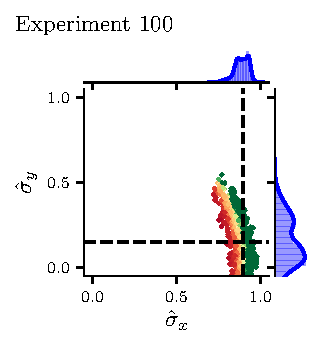
\includegraphics{algorithms/figures/smc_demo/epoch_100.pdf}
    }
    \subfloat{ 
    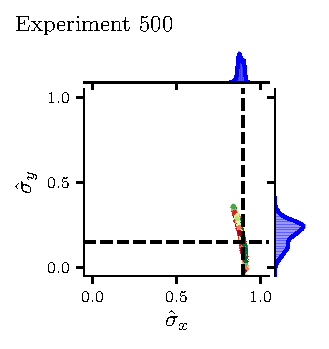
\includegraphics{algorithms/figures/smc_demo/epoch_500.pdf}
    }
    % \hspace{0mm}
    \subfloat{
        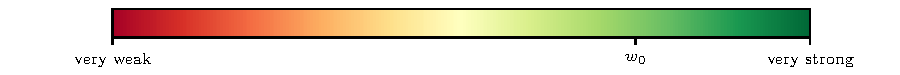
\includegraphics{algorithms/figures/smc_demo/cbar.pdf}
    }
    \caption[Quantum Hamiltonian learning via sequential Monte carlo]{
    \Acrfull{qhl} via \acrfull{smc}. 
    The studied model has two terms, $\{\sx, \sy\}$ with true parameters $\alpha_{x}=0.9, \alpha_y=0.15$ (dahsed lines), 
        with $\Ne=500, \Np=2000$. 
    Crosses represent particles, while the distribution $\Pr(\alpha_p)$ for each 
        parameter can be seen along the top and right-hand-sides of each subplot. 
    Both parameters are assigned a uniform probability distribution $\mathcal{U}(0,1)$, representing our prior knowledge of the system. 
    \textbf{(a), }\gls{smc} samples $\Np$ particles from the initial joint probability distribution, 
        with particles uniformly spread across the unit square, each assigned the starting \emph{weight} $w_0$. 
        At each experiment $e$, each of these particles' likelihood is computed according to \cref{eqn:particle_bayes_rule}
        and its weight is updated by \cref{eqn:qhl_weights}.
    \textbf{(b),} after 9 experiments, the weights of the sampled particles are sufficintly informative that we know we can 
        discard some particles while most likely retaining the true parameters. 
    \textbf{(c),} \gls{smc} resamples according the current $\Pr(\al)$, 
        i.e. having accounted for the experiments and likelihoods observed to date, 
        a new batch of $\Np$ particles are drawn, and each reassigned weight $w_0$, 
        irrespective of their weight prior to resampling.  
    \textbf{(d, e),} Afer further experiments and resamplings, \gls{smc} narrows $\Pr(\al)$ to a region around the true parameters. 
    \textbf{(f),} The final \emph{posterior} distribution consists of two narrow distributions centred on $\alpha_x$ and $\alpha_y$. 
    }
    \label{fig:qhl_smc}
\end{figure}

In practice, \gls{qhl} samples from and updates $\Pr(\al)$  via \gls{smc}.
\gls{smc} samples the $\Np$ particles from $\Pr(\al)$, and assigns each particle a weight, $w_0 = 1/\Np$.
Each particle corresponds to a unique position in the parameters' space, i.e. $\al_p$.
Following the calculation of the likelihood, $\Pr(d | \al_p; e)$, 
    the weight of particle $p$ are updated by \cref{eqn:qhl_weights}.
\begin{equation}\label{eqn:qhl_weights}
    w_p^{new} = \frac{\Pr(d | \al_p; e) \times w_p^{old} } { \sum\limits_{p} w_p \Pr(\al_p | d; e) }
\end{equation}

In this way, strong particles (high $\Pr(d | \al_p; e)$) have their weight increased, 
    while weak particles (low $\Pr(d | \al_p; e)$) have their weights decreased, 
    and the sum of weights remains normalised. 
Within a single experiment, the weights of all $\Np$ particles are updated thus:
    we \emph{simulataneously} update sampled particles' weights as well as $\Pr(\al)$. 
This iterates for the following experiment, using the \emph{same} particles: 
    we do \emph{not} redraw $\Np$ particles for every experiment.
Eventually, the weights of most particles fall below a threshold, $r_t$, 
    meaning that only that fraction of particles have reasonable likelihood of being $\al_0$.
At this stage, \gls{smc} \emph{resamples}, i.e. selects new particles, according to the updated $\Pr(\al)$,
    according to the Liu-West resampling algorithm \cite{liu2001combined}.
Then, the new particles are in the range of parameters which is known to be more likely, 
    while particles in the region of low-weight are effectively discarded. 
Usually, we set $r_t=0.5$, although this \gls{hyperparameter} can have a large impact 
    on the rate of learning, so can be optimised in particular circumstances, 
    see \cref{fig:param_learning_vary_particles}.
This procedure is easiest understood through the example presented in \cref{fig:qhl_smc}, 
    where a two-parameter Hamiltonian is learned starting from a uniform distribution. 


\section{Likelihood}\label{sec:likelihood}
The fundamental step within \gls{qhl} is the calculation of \gls{likelihood} in \cref{eqn:particle_bayes_rule}. 
The core of this learning algorithm is that this \gls{likelihood} can be retrieved from the Born rule, 
    although in principle \emph{any} valid likelihood function can fulfil this equation, 
    provided the calculation of the likelihood captures the probabilty that the present hypothesis produced the present datum.

In general, it is not always possible to derive the analytical likelihood, 
    especially in cases where we wish to vary the \gls{probe}.
When \cref{eqn:likelihood} can be computed classically, 
    \gls{qhl} relies on \gls{cle}, i.e. involving the exponential calculation of \cref{eqn:likelihood}, 
    whereas \gls{qle} uses the same likelihood function computed on a quantum simulator; 
    this is the sole application of quantum simulators in this protocol and indeed the remainder of this thesis. 
Access to such hardware, operating perfectly, would provide exponential speedup in the calculation of this term, 
    rendering both \gls{qhl} and the wider \gls{qmla} formalism scalable,
    although in this thesis we do not implement \gls{qle} so everything can be viewed as \gls{cle}. 
\gls{qle} was implemented in \cite{wang2017experimental}. 
\par 

We adopt notation used by QInfer, which \gls{qmla} for the likelihood estimation stage \cite{qinfer-1_0}. 
The expectation value for a the unitary operator is given by
\begin{equation}\label{eqn:pr0}
    \Pr(0) =  |\bra{\psi} e^{-i \hat{H}_p t} \ket{\psi}|^2  = l(d=0 | \hat{H}_p; e), 
\end{equation}
    i.e. the input basis is assigned the measurement label $d=0$, and this quantity is the probability 
    of measuring $d=0$, i.e. measuring the same state as input. 
However, we assume a binary outcome model, 
    i.e. that the system is measured either in $\ket{\psi}$ (labelled $d=0$), or it is not ($d=1$);
    the likelihood for the latter case is
\begin{equation}\label{eqn:pr1}
    \Pr(1) = l(d=1 | \hat{H}_p; e) = \sum_{\{\ket{\psi_{\perp}}\}} | \bra{\psi_{\perp}} e^{-i \hat{H}_p t} \ket{\psi}  |^2 = 1 - \Pr(0).
\end{equation}
\par 
Usually we will refer to the case where $Q$ is projeced onto the input state $\ket{\psi}$, 
    so the terms \emph{likelihood}, \emph{expectation value} and \emph{$\Pr(0)$} are synonymous, 
    unless otherwise stated. 


\subsection{Interactive Quantum Likelihood Estimation}\label{sec:iqle}
An important extension to \gls{qle} is \gls{iqle}, 
    which follows \gls{smc} but uses an alternative \gls{likelihood} function in order to 
    overcome some of its inherent challenges \cite{Wiebe:2014qhl}. 
Two almost identical Hamiltonians will diverge after exponentially small evolution time \cite{jalabert2001environment}.
This is problematic for \gls{qhl} because it relies on the likelihood function which is built on the assumption 
    that increasing accuracy of $\ha$ approximating $\ho$ should result in rising likelihood;
    this result indicates that even extremely accurate approximations become unreliable after very short evolution times. 
Coupled with the result that small time experiments are uninformative \cite{wiebe2015quantum}, 
    this observation demands exponentially many measurements to approximate the exponentially small likelihoods, 
    rendering the approach inefficient. 
\par 
The \gls{le} is the measure of the revival resulting from an imperfect time-reversal operation implemented after the standard time evolution. 
The reversal operation corresponds to some Hamiltonian, $\hat{H}_{-}$, which is seen as an attempt to un-do the evolution
    according to the original Hamiltonian, $\hat{H}_{+}$. 
As such we say that $\hat{H}_{-}$ is evolved for $-t$, so its unitary is $e^{-i \hat{H}_{-}(-t)}$ after $\hat{H}_{+}$ is evolved for $t$. 
The \gls{le} can be written and characterised as 
\begin{align}
    \label{eqn:loschmidt_echo}
    M(t) = \absval{ \braket{ \psi | e^{+i\hat{H}_{-} t} e^{-i \hat{H}_{+} t} | \psi} }^2 \sim 
    \begin{cases}
        1 - \mathcal{O}(t^2),  & t \leq t_c \\
        e^{-\mathcal{O}(t)}, & t_c \leq t \leq t_{s} \\
        \nicefrac{1}{\| \hat{H} \|}, & t \geq t_{s}
    \end{cases}
\end{align}
    where $\hat{H}_{-}, \hat{H}_{+}$ are backward and forward time evolutions respsectively, which are assumed almost identical;
    $\|\hat{H}\|$ is their dimension, and $t_c, t_{s}$ are bounds on the evolution time marking the transition between the 
    \emph{parabolic decay}, \emph{asymptotic decay} and \emph{saturation} of the echo \cite{goussev2012loschmidt}. 
In effect, the \gls{le} gaurantees that if $\hat{H}_{-} \not\approx \hat{H}_{+}$, then $M(t) \ll 1$, 
    while $\hat{H}_{-} \approx \hat{H}_{+}$ gives $M(t) \approx 1$. 
This can be exploited for learning: 
    by taking $\hat{H}_{+}$ as either $\ho$ (true) or $\ha$ (particle or hypothesis), 
    and sampling $\hat{H}_{-}$ from $\pra$, 
    we can adopt \cref{eqn:loschmidt_echo} as the likelihood function in \cref{eqn:likelihood}, 
    in the knowledge that this will disinguish between hypotheses based on their similarity to $\ho$.
\par 

Importantly, \gls{iqle} can only be used where we can \emph{reliably} evolve the system under study. 
In order that the reverse evolution is relibable, it must be performed on a trusted simulator, 
    restricting \gls{iqle} to cases where a coherent quantum channel exists between the target
    system and a trusted simulator. 
This automatically excludes any open quantum systems, as well as most realistic 
    experimental setups, although such channels can be achieved \cite{hensen2015loophole}. 
The remaining application for \gls{iqle}, and correspondingly \gls{qhl}, 
    is in the characterisation of untrusted quantum simulators, 
    which can realise such coherent channels \cite{wang2017experimental}. 

\subsection{Analytical likelihood}    
In some cases, analytical likelihood functions can be derived to describe the dynamics of simple quantum systems 
    \cite{sergeevich2011characterization, ferrie2013best},
    for instance encoding the Rabi frequency $\omega$ of an oscillating electron spin in an \gls{nvc},
    \begin{equation}
        \label{eqn:analytical_hamiltonian}
        \hat{H}(\omega) = \frac{\omega}{2} \s_z.
    \end{equation}
Then, bearing in mind that $\s_z \s_z = \hat{\mathbb{1}}$, so $\s_z^{2k}=\hat{\mathbb{1}}$ and $\s_z^{2k+1} = \s_z$, 
    using MacLaurin expansion, the unitary evolution of \cref{eqn:analytical_hamiltonian} is given by 
\begin{align}
    \begin{split}
        U = e^{-i \hat{H}(\omega)t} = e^{-i \frac{\omega t}{2} \s_z}  
        &= \cos\bk{ \frac{\omega t \s_z}{2}} 
        - i \sin\bk{ \frac{\omega t \s_z}{2}} \\
        &= \bk{ \sum\limits_{k=0}^{\infty} \frac{(-1)^k}{(2k)!} \bk{ \frac{\omega t}{2} }^{2k} \s_z^{2k}  }
        - i \bk{\sum\limits_{k=0}^{\infty} \frac{(-1)^k}{(2k+1)!} \bk{ \frac{\omega t}{2} }^{2k+1} \s_z^{2k+1}} \\
        &=  \bk{\sum\limits_{k=0}^{\infty} \frac{(-1)^k}{(2k)!} \bk{ \frac{\omega t}{2} }^{2k+1}} \hat{\mathbb{1}} 
        - i \bk{\sum\limits_{k=0}^{\infty} \frac{(-1)^k}{(2k+1)!} \bk{ \frac{\omega t}{2} }^{2k+1} } \s_z \\
        &= \cos\bk{\frac{\omega t}{2}}\hat{\mathbb{1}} - i \sin\bk{\frac{\omega t}{2}} \s_z
    \end{split}
\end{align}
    
Then, evolving a \gls{probe} $\ket{\psi_0}$ and projecting onto a state $\ket{\psi_1}$ gives
\begin{equation}
    \label{eqn:rabi_projection}
    \bra{\psi_1} U \ket{\psi_0} = \cos\bk{\frac{\omega t}{2}} \braket{\psi_1 | \psi_0} - i \sin\bk{\frac{\omega t}{2}} \braket{ \psi_1 | \s_z | \psi_0}.
\end{equation}
By initialising and projecting into the same state, say $\ket{\psi_0} = \ket{\psi_1} = \ket{+}$, we have
\begin{align}
    \begin{split}
        \s_z\ket{+} = \ket{-} \implies \braket{\psi_1 | \s_z | \psi_0} &= 0 \\
        \braket{\psi_1 | \psi_0} &= 1 \\
        \implies \braket{\psi_1 |  U | \psi_0} &= \cos\bk{\frac{\omega t}{2}},
    \end{split}
\end{align}
    i.e. if the system measures in $\ket{+}$, we set the datum $d=1$, otherwise $d=0$. 
Then, from Born's rule, and in analogy with \cref{eqn:likelihood}, we can formulate the likelihood function, 
    where the hypothesis is the single parameter $\omega$, and the sole experimental control is $t$, 
\begin{equation}
    \label{eqn:analytical_likleihood}
    \Pr(d=1 | \omega; t) = \left| \braket{\psi_1 |  U | \psi_0} \right|^2 = \cos^2\bk{\frac{\omega t}{2}}
\end{equation}
This analytical likelihood will underly the simulations used in the following introductions, except where explicitly mentioned. 

\section{Total log total likelihood}\label{sec:total_log_total_likelihood}
We have already used the concept of \gls{likelihood} to update our parameter distribution during \gls{smc}; 
    we can consolidate the likelihoods of all particles with respect to a single datum, $d$, from a single experiment $e$,  
    in the \emph{total likelihood}, 
    \begin{equation}
        \label{eqn:total_likelihood}
        \lk_{e} = \sum\limits_{p \in \{p\}} \Pr(d | \al_p ; e) \times w_p^{old}.
    \end{equation}
For each experiment, we use total likelihood as a measure of how well the distribution performed,
    i.e. we care about how well all particles, $\{p\}$, perform as a collective, representative of how well $\Pr(\al)$ approximates the system,
    equivalent to the noramlisation factor in \cref{eqn:qhl_weights}, \cite{granade2015characterizationp92}. 

$\lk_{e}$ are strictly positive, and because the natural logarithm is a monotonically increasing function, 
    we can equivalently work with the \gls{ltl}, 
    since $ln(\lk_a) > ln(\lk_b) \iff \lk_a > \lk_b$. 
\gls{ltl} are also beneficial in simplifying calculations, 
    and are less susceptible to system underflow, 
    i.e. very small values of $\lk$ will exhaust floating point precision, 
    but $ln(\lk)$ will not. 
\par 

Note, we know that
\begin{align}    
    \begin{split}
        w_p^0 = \frac{1}{\Np} & \implies \sum_p^{\Np} w_p^0 = 1 ; \\
        \Pr(d | \al_p; e) \leq 1 & \implies \Pr(d | \al_p; e) \times w_p^{old} \leq w_p^{old} \\
        & \implies \sum\limits_{\{p\}} \Pr(d | \al_p; e) \times w_p^{old} \leq \sum\limits_{\{p\}} w_p^{old} \leq \sum_p^{\Np} w_p^0; \\
        & \implies \lk_{e} \leq 1.
    \end{split}
\end{align}

\cref{eqn:total_likelihood} essentially says that a good batch of particles, 
    where on average particles perform well, 
    will mean that most $w_i$ are high, so $\lk_{e} \approx 1$. 
Conversely, a poor batch of particles will have low average $w_i$, so $\lk_{e} \approx 0$. 
\par

In order to assess the quality of a \emph{model}, $\hi$, 
    we can consider the performance of a set of particles throughout a set of experiments $\expset$, 
    through its \gls{tltl}, 
\begin{equation}
    \label{eqn:log_total_likelihood}
    \tll_{i} = \sum\limits_{e \in \expset} ln(\lk_{e}).    
\end{equation}

The set of experiments on which $\tll_{i}$ is computed, $\expset$, 
    as well as the particles whose sum constitute each $\lk_{e}$
    can be the same experiments on which $\hi$ is trained, $\expset_i$, but in general need not be, 
    i.e. $\hi$ can be evaluated by considering different experiments than those on which it was trained.
For example, $\hi$ can be trained with $\expset_i$ to optimise $\al_i^{\prime}$, 
    and thereafter be evaluated using a different set of experiments $\expset_v$, 
    such that $\tll_{i}$ is computed using particles sampled from the distribution after optimising $\al$, 
    $\Pr(\al_i^{\prime})$, and may use a different number of particles than the training phase. 

Perfect agreement between the model and the system would result in $\lk_{e}=1 \Rightarrow ln(\lk_{e})=0$, 
    as opposed to poor agreement $\lk_{e} < 1 \Rightarrow ln(\lk_{e}) < 0$.
Then, in all cases \cref{eqn:log_total_likelihood} is negative, 
    and across a series of experiments,
    strong agreement gives low $\left| \tll_{i} \right| $, 
    whereas weak agreement gives large $\left| \tll_{i} \right| $. 


\section{Parameter estimation}

\begin{figure}[t]
    \centering
    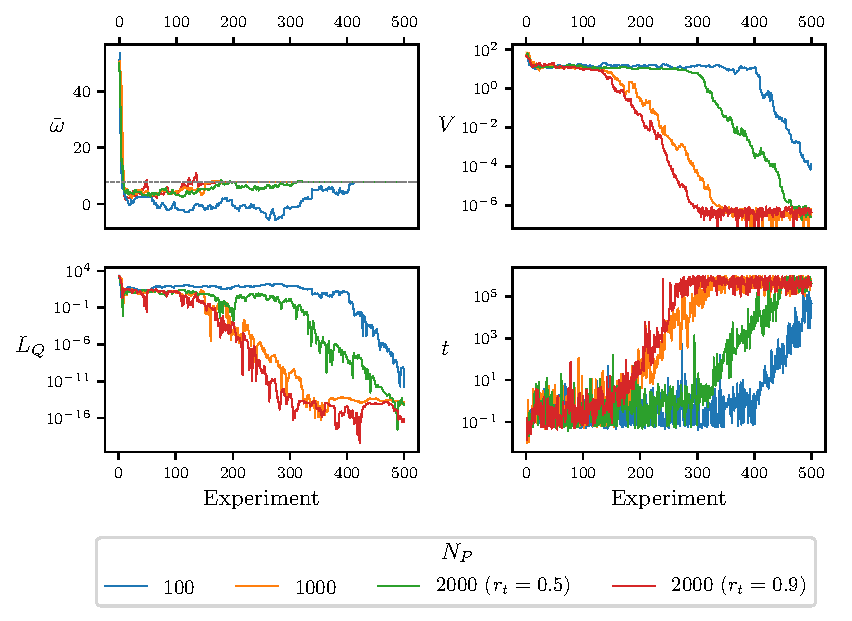
\includegraphics{algorithms/figures/params.pdf}
    \caption[Parameter learning varying number of particles]{
        Parameter learning for the analyitcal likelihood \cref{eqn:analytical_likleihood}
        for varying numbers of particles $\Np$, for $\Ne=500$. 
        For $\Np=2000$, we show the resampler threshold set to $r=0.5$ and $r=0.9$. 
        (a) the parameter estimate, i.e. $\bar{\omega}$, the mean of the posterior distribution after each experiment, 
        approaching $\omega_0=7.75$ (dashed line), where the prior is centred on $\omega=50 \pm 25$. 
        Decrease in (b) volume, $V$, (c) quadratic loss, $L_Q$, 
        and (d) evolution time, $t$, are shown against experiment number.
    }
    \label{fig:param_learning_vary_particles}
\end{figure}


\gls{qhl} is a parameter estimation algorithm, so here we introduce some methods to evaluate its performance, 
    which we can reference in later sections of this thesis. 
\par 
The most obvious meausre of the progression of parameter estimation is the error between the true parameterisation, 
    $\al_0$, and the approximation $\al_p = \mean \bk{ \Pr(\al) }$,
    which can be captured by a large family of loss functions. 
Here we use the \gls{ql}, which captures this error through the sum of the square difference between 
    each parameter's true and estimated values symetrically, 
    i.e. error above the true parameter is as impactful as error below. 
We can record the \gls{ql} at each experiment of our training regime and hence track its performance. 
\begin{definition}[Quadratic Loss]
    \label{def:quadratic_loss}
    For a true parameterisation $\al_0$, and a hypothesis $\al$, the quadratic loss is given by
    \begin{equation}
        \label{eqn:quadratic_loss}
        L_{Q} = \left\| \al_0 - \al \right\|^2.
    \end{equation}
\end{definition}
\par 

\subsection{Volume}\label{sec:volume}
We also care about the range of parameters supported by $\Pr(\al)$ at each experiment: 
    the \gls{volume} of the particle distribution can be seen as a proxy for our certainty
    that the approximation $\mean\bk{\Pr(\al)} $ is accurate. 
For example, for a single parameter $\omega$, our best knowledge of the parameter is $\mean\bk{ \Pr(\omega) }$, 
    and our belief in that approximation is the standard deviation of $\Pr(\omega)$; 
    we can think of volume as an $n$-dimensional generalisation of this intuition \cite{qinfer-1_0, ferrie2014high}. 
\par 
In general, a confidence region, defined by its confidence level $\kappa$, is drawn by grouping particles 
    of \gls{hpd}, $\mathcal{P}$, such that $\sum\limits_{p \in \mathcal{P}} w_{p} \geq \kappa$.
We use the concept \todo{do we use MVEE or the posterior directly as the credible region?} of \gls{mvee} 
    to capture the confidence region \cite{ferrie2014high}, calculated as in \cite{todd2007khachiyan}, 
    which are characterised by their covariance matrix, $\Sigma$, which allows us to calculate the \gls{volume}, 
    \begin{equation}
        \label{eqn:volume}
        V(\Sigma) = \frac{ \pi^{| \al | / 2}}{ \Gamma(1 + \frac{| \al |}{2})} \det\bk{\Sigma^{-\frac{1}{2}}},
    \end{equation}}
    where $\Gamma$ is the Gamma function, and $|\al|$ is the cardinality of the parameterisation. 
This quantity allows us to meaningfully compare distributions of different dimension, 
    but we must be cautious of drawing strong comparisons between models based on 
    their volume alone, for instance because they may have started from vastly different prior distributions. 
\par 

Within \gls{smc}, we assume the credible region is simply the posterior distribution, 
    such that we can take $\Sigma = \textrm{cov}(\Pr(\al))$ after each experiment, 
    and hence track the uncertainty in our parameters across the training experiments \cite{Granade:2012kj}.
We use volume as a measure of the learning procedure's progress: 
    slowly decreasing or static volume indicates poor learning, possibly highlighting poor experiment design, 
    while fast or exponentially decreasing volume indicates that the parameters are being learned well. 
When the volume has converged, the learning has saturated and there is little benefit to running further experiments. 

\section{Experiment design heuristic}
\label{sec:heuristic}
A key consideration in \gls{qhl} is the choice of experimental controls implemented in attempt to learn from the system. 
The experimental controls required are dictated by the choice of \gls{likelihood} function used within \gls{smc}, 
    though typically there are two primary controls we will focus on: 
    the evolution time, $t$, and the \gls{probe} state evolved, $\ket{\psi}$. 
The design of experiments is handled by an \gls{edh}, 
    whose structure can be altered to suit the user's needs. 
Usually, the \gls{edh} attempts to exploit the information available, 
    adaptively accounting for some aspects of the inference process performed already, 
    although there may be justification for enforcing a non-adaptive schedule, 
    for instance to force \gls{qhl} to train on a full set of experimental data 
    rather than a restricted set which adaptive methods would advise.
We can categorise each \gls{edh} as either \emph{online} of \emph{offline},
    depending on whether it accounts for the current state of the inference procedure, i.e. the posterior.
The \gls{edh} is modular and can be replaced by any method that returns a valid set of experimental controls, 
    so we can consider numerous approaches, for instance those described in \cite{hincks2018hamiltonian, fiderer2020neural}.
\par 

\subsection{Particle Guess Heuristic}\label{sec:pgh}
The default \gls{edh} is the \gls{pgh} \cite{Wiebe:2014qhl}, 
    an online method which attempts to design the optimal evolution time based on the posterior.
Note \gls{pgh} does not specify the \gls{probe}, so is coupled with a \gls{probe} selection routine to comprise 
    a complete \gls{edh}.
\par

The principle of \gls{pgh} is that the uncertainty of the posterior limits how well the Hamiltonian is currently 
    approximated, and therefore limits the evolution time for which the posterior can be expected to 
    reasonably mimic $\ho$.
For example, consider \cref{eqn:analytical_hamiltonian} with a single parameter with $\omega_0 = 10$,
    and current $\mean\bk{\Pr(\omega)} = 9, \std\bk{\Pr(\omega)} = 2$, 
    we can expect that the approximation $\omega^{\prime} = \mean\bk{\Pr(\omega)}$ 
    is valid up to $t_{max} = \nicefrac{1}{\std\bk{\Pr(\omega)}}$. 
% TODO make a figure illustrating this point with some wide, medium and thin priors
It is sensible, then, to use $t \sim t_{max}$ for two reasons: 
    (i) smaller times are already well explained by the posterior, so offer little opportunity to learn;
    (ii) $t_{max}$ is at or near the threshold the posterior can comfortably explain, 
        so it will expose the relative difference in likelihood between the posterior's particles, 
        providing a strong capacity to learn. 
Informally, as the uncertainty in the posterior shrinks, \gls{pgh} selects larger times 
    to ensure the training is based on informative eperiments simulataneously with increasing 
    certainty about the paraemters. 
In the one-dimensional case, this logic can be used to find an optimal time heuristic, 
    where experiment $k$ is assigned $t_k = \nicefrac{1.26}{\std\bk{\Pr(\omega)}}$ \cite{ferrie2013best}. 
\par
Rather than directly using the inverse of the standard deviation of $\pr{\al}$, 
    which relies on the expensive calculation of the covarinace matrix, 
    \gls{pgh} uses a proxy whereby two particles are sampled from $\pr{\al}$. 
The experimental evolution time for experiment $k$ is then given by 
\begin{equation}
    \label{eqn:pgh_time}
    t_k = \frac{1}{\| \al_i - \al_j \|}, 
\end{equation}
    where $\al_i, \al_j$ are distinct particles sampled from $\mathcal{P}$ where 
    $\mathcal{P}$ is the set of particles under consideration by \gls{smc} after experiment $k-1$, 
    which had been recently sampled from $\Pr\bk{\al}$. 
\par 


\subsection{Alternative experiment design heuristics}\label{sec:alt_heuristics}
The \gls{edh} can be used to suit the requirements of the target system; 
    we test four such examples against a series of models. 
Here the \gls{edh} must only design the evolution time for the experiment, 
    with probe design discussed in the next section. 
The heuristics tested are:

\begin{easylist}
    \ListProperties(Numbers=r)
    & $\textrm{Random}(0, t_{max})$: Randomly chosen time up to some arbitrary maximum, we set $t_{max} = 1000$. 
        This approach is clearly subobtimal, since it does not account whatsoever for the knowledge of the training so far, 
        and demands the user choose a suitable $t_{max}$, which is not gauranteed to be meaningful. 
    & $t$ list: forcing the training to consider a set of times decided in advance.
        For instance, when only a small set of experimental measurements are available, it is sensible to train on all of them, perhaps repeatedly. 
        We test uniformly spaced times between 0 and $t_{max}$, and train on the list twice.
        Again this \gls{edh} fails to account for the performance of the trainer so far, so may use times either 
        far above or below the ability of the parameterisation. 
    & $(\nicefrac{9}{8})^k$: An early attempt to match the expected exponential decrease in volume from the training, 
        was to set $t = (\nicefrac{9}{8})^k$ \cite{Granade:2012kj}.
        Note we increment $k$ after 10 experiments in the training regime, 
        rather than after each experiment, which would result in extremely high times which flood memory.
    & \Gls{pgh}: as in \cref{sec:pgh}. 
\end{easylist}

We show how the choie of \gls{edh} within this set can influence the training procedure,
    by testing models of various complexity amd dimension. 
In particular, we first test a simple 1-qubit model, \cref{eqn:qhl_test_model_1}; 
    followed by more complicated 1-qubit model, \cref{eqn:qhl_test_model_2};
    as well as randomly generated 5-qubit Ising, \cref{eqn:qhl_test_model_3}, and 4-qubit Heisenberg models, \cref{eqn:qhl_test_model_4}.
Each $\hi$ have randomly chosen parameters implicitly assigned to each term. 
\begin{subequations}\label{eqn:qhl_test_models}
    \begin{equation}
        \label{eqn:qhl_test_model_1}
        \h_1=\s^z_1
    \end{equation}
    \begin{equation}
        \label{eqn:qhl_test_model_2}
        \h_2 = \s^x_1 + \s^y_1 + \s^z_1
    \end{equation}
    \begin{equation}
        \label{eqn:qhl_test_model_3}
        \h_3 = \s^z_1\s^z_3 + \s^z_1\s^z_4 + \s^z_1\s^z_5 + \s^z_2\s^z_4 +\s^z_2\s^z_5 + \s^z_3+\s^z_4 + \s^z_3+\s^z_5
    \end{equation}
    \begin{equation}
        \label{eqn:qhl_test_model_4}
        \h_4 = \s^z_1\s^z_2 + \s^z_1\s^z_3 +\s^x_2\s^x_3 + \s^z_2\s^z_3 + \s^x_2\s^x_4 + \s^z_3\s^z_4
    \end{equation}
\end{subequations}

\begin{figure}
    \begin{center}
        \QMLAfig{Nov_27/heuristic_comparisons.pdf}
    \end{center}
    \caption[Training with different heuristics]{
        The volume of various models when trained through \gls{qhl} using different \glspl{edh}.
        We show models of various complexity and dimension, each trained using four heuristics, 
        outlined in the main text.
        \figtableref
    }
    \label{fig:heuristics_test}
\end{figure}

We show the performance of each of the listed \glspl{edh} in \cref{fig:heuristics_test}. 
We will have cause to use alternative \glspl{edh} in paricular circumstances, 
    but we adopt \gls{pgh} as the default \gls{edh} throughout this thesis, 
    unless otherwise stated.


\section{Probe selection}

A final consideration for experiments within \gls{qhl} is the choice of input \gls{probe} state, $\ket{\psi}$,
    which is evolved in the course of finding the likelihood used during the Bayesian update. 
We can consider the choice of probe as an output of the \gls{edh},  
    although previous work has usually not considered optimising the \gls{probe}, 
    instead usually setting $\ket{\psi} = \ket{+}^{\otimes n}$ for $n$ qubits \cite{wang2017experimental, ferrie2013best}.
In principle it is possible for the \gls{edh} to design a new \gls{probe} at each experiment, 
    although a more straightforward approach is to compose a set of probes offline, $\Psi = \{ \ket{\psi} \}$,
    of size $\Npsi = \absval{\Psi}$.
Then, a probe is chosen at each experiment from $\Psi$, 
    allowing for the same $\ket{\psi}$ to be used for the multiple experiments within the training, e.g. by iterating over $\Psi$. 
$\Psi$ can be generated with respect to the individual learning problem as we will examine later, 
    but it is usually sufficient to use generic strategies which should work for all models;
    some straightforward examples are
    \begin{easylist}[enumerate]
        \ListProperties(Numbers=r)
        & $\ket{0} : \ \Psi = \{\ket{0}^{\otimes n}\}, \ \ \Npsi=1$;
        & $\ket{+} : \ \Psi = \{\ket{+}^{\otimes n}\}, \ \ \Npsi=1$;
        & $\ket{t} : \ \Psi$ is the tomographic basis set, \ \ $\Npsi=40$;
        & $\ket{r} : \ \ket{\psi}$ are random, separable probes, \ \ $\Npsi=40$.
    \end{easylist}
\par 
We show the 1-qubit probes within $\Psi$ under each of these strategies on the Bloch sphere in \cref{fig:probes_used_bloch}.

\begin{figure}
    \begin{center}
        \subfloat{
            % 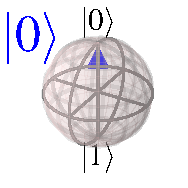
\includegraphics[width=0.2\textwidth]{qmla_run_data/Nov_27/zero_probes.pdf}
            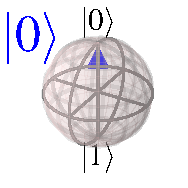
\includegraphics{qmla_run_data/Nov_27/zero_probes.pdf}
        }
        \qquad
        \subfloat{
            % 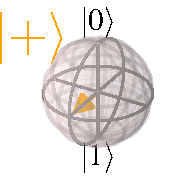
\includegraphics[width=0.2\textwidth]{qmla_run_data/Nov_27/plus_probes.pdf}
            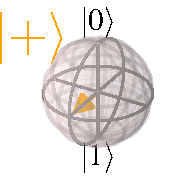
\includegraphics{qmla_run_data/Nov_27/plus_probes.pdf}
        }
        \qquad
        \subfloat{
            % 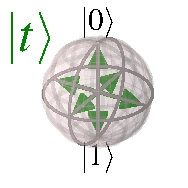
\includegraphics[width=0.2\textwidth]{qmla_run_data/Nov_27/tomographic_probes.pdf}
            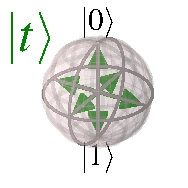
\includegraphics{qmla_run_data/Nov_27/tomographic_probes.pdf}
        }
        \qquad
        \subfloat{
            % 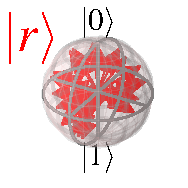
\includegraphics[width=0.2\textwidth]{qmla_run_data/Nov_27/random_probes.pdf}
            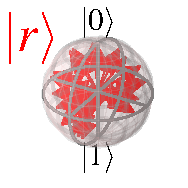
\includegraphics{qmla_run_data/Nov_27/random_probes.pdf}
        }
        \qquad
    \end{center}
    \caption[Probes used for tests]{
        1-qubit probes used for tests in \cref{fig:probes_test}.
    }
    \label{fig:probes_used_bloch}
\end{figure}

\begin{figure}
    \begin{center}
        \QMLAfig{Nov_27/training_probes.pdf}
    \end{center}
    \caption[Training with different probes]{
        The volume of various models when trained through \gls{qhl} using different initial \gls{probe} sets. 
        We show models of various complexity and dimension, each trained using random probes, $\ket{r}$, 
        tomographic basis set probes, $\ket{t}$, as well as $\ket{0}$ and $\ket{+}$ probes. 
        In each case the probes are generated for arbitrary numbers of qubits; 
        for $\ket{0}, \ket{1}$, the number of probes generated is $N_{\psi}=1$, 
        and for $\ket{t}, \ket{r}$, $N_{\psi}=40$.
        \figtableref
    }
    \label{fig:probes_test}
\end{figure}

We test the same set of models as \cref{eqn:qhl_test_models} and test each of these \gls{probe} construction 
    strategies in \cref{fig:probes_test}. 
We can draw a number of useful observations from these simple tests: 
\begin{easylist}[itemize]
    & Training on an eigenstate, $\ket{0}$, of the model yields no information gain. 
        This is because all particles give likelihoods $l=1$, 
    so no weight update can occur, meaning the parameter distribution does not change when presented new evidence. 
    & Training on an even superposition of the model's eigenstates, $\ket{+}$, is maximally informative: 
        any deviations from the true parameterisation are registered most dramatically in this basis,
        providing the optimal training probe for this case.     
    & These observations are reinforced by \cref{fig:probes_test}\textbf{c}, where a 5-qubit Ising model also 
        fails to learn from one of its eigenstates, $\ket{0}^{\otimes 5}$.
        Of note, however, is that $\ket{+}^{\otimes 5}$ is not the strongest probe here: the much larger Hilbert space here 
        can not be scanned sufficiently using a single probe; 
        using a larger number of probes is more effective, even if those are randomly chosen. 
    & In general the tomographic and random probe sets perform reliably. 
\end{easylist}

It is an open challenge to identify the optimal probe for training any given model, 
    and the choice of such informative probes could be built into the \gls{edh} in general, 
    for example by computing the eigenstates of the candidate, and generating a probe set
    from superposition between those eigenstates. 
However, a further consideration is that, for model comparison purposes, 
    it is helpful to have a universal set of probes, upon which all models are learned. 
This would minimise bias towards particlar models, which might arise from probes which are favourable bases 
    for a subset of models, for example $\ket{+}$ in \cref{fig:probes_test}\textbf{a}. 
Careful consideration should be given to $N_{\psi}$ in the choice of the probe generator, 
    since it is important to ensure probes test the parameterisation across the Hilbert space robustly, 
However this must be balanced by ensuring \gls{smc} has sufficient opportunity to learn within a subspace before moving to the next; 
    we can mitigate this concern by instructing the \gls{edh} to repeatedly select a probe from $\Psi$ for a batch of experiments, 
    say five, before moving to the next available probe. 
\par 

As standard for the remainder of this thesis, unless otherwise stated, 
    we adopt the random probe generator as the defualt mechanism for selecting probes,
    only iterating between probes after batches of 5 experiments.

    \chapter{Quantum Model Learning Agent}\label{chapter:qmla}
        \glsreset{qmla}
\gls{qmla} is an algorithm that extends the concept of applying machine learning to the 
    characterisation of Hamiltonians we've seen so far. 
The extension, and central question of \gls{qmla} is:
    if we do not even have the structure of the model which describes a target quantum system, 
    can we still learn about the physics of the system?
That is, we remove the assumption about the form of the Hamiltonian model, 
    and attempt to uncover which \emph{\glspl{term}} constitute the Hamiltonian, 
    and in so doing, learn what interactions the system is subject to. 
Throughout this thesis, we are concerned solely with Hamiltonian models. 
    although, in general, the description of a quantum system of interest need not be Hamiltonian, 
    e.g. it could be Lindbladian for open quantum systems, 
    so we generalise the effort to the search for the most suitable \emph{\gls{model}}. 
\par 

For the remainder of this thesis, our objective is to learn the model underlying 
    some target system $Q$. 
We will first introduce some concepts which will prove useful when discussing \gls{qmla}, 
    before describing the protocol in detail in \cref{sec:qmla_protocol}.


    

%%%%%%%%%%% MODELS %%%%%%%%%%% 
\section{Models}\label{sec:models}
\Glspl{model} are simply the mathematical objects which can be used to predict the behaviour of a system. 
In this thesis, \glspl{model} are synonymous with Hamiltonians,
    composed of a set of \emph{}\glspl{term}}, $\termset = \{ \hat{t}\}$, 
    where each $\hat{t}$ is a matrix. 
Each term is assosiated with a multipicative scalar, which may be referred to as that term's \emph{parameter}: 
    we impose order on the terms and parameters such that we can succinctly summarise any model as 

\begin{align}
    \label{eqn:model}
    \begin{split}
        \hat{H} = \irow{\alpha_0 & \dots & \alpha_n} \icol{\hat{t}_1 \\ \vdots \\ \hat{t}_n} = \al \cdot \terms 
    \end{split}
\end{align}
    where $\al, \terms$ are the model's parameters and terms, respectively.

For example, a model which is the sum of the (non-identity) Pauli operators is given by
\begin{align}
    \label{eqn:pauli_sum_model}
    \begin{split}
        \hat{H} &= \irow{\alpha_x & \alpha_y & \alpha_z} \cdot \icol{\sx \\ \sy \\ \sz} \\
        &= \alpha_x \sx + \alpha_y \sy + \alpha_z \sz \\
        &= \begin{pmatrix}
            \alpha_z & \alpha_x - i \alpha_y \\
            \alpha_x + i\alpha_y & \alpha_z
        \end{pmatrix}.
    \end{split}
\end{align}
\par 

Through this formalism, we can say that the sole task of \gls{qhl} was to optimise $\al$, given $\terms$. 
The principle task of \gls{qmla} is to identify $\terms$ with the most statistical evidence 
    for describing the target system $Q$. 
In short, \gls{qmla} proposes candidate models $\hi$ as hypoteses to explain $Q$; 
    we \emph{train} each model independently through a parameter learning routine, 
    and finally nominate the model with the best performance after training. 
In particular, \gls{qmla} uses \gls{qhl} as the parameter learning subroutine, 
    but in principle this step can be performed by any algorithm which learns $\al$ for given $\terms$, 
    such as tomography \cite{wang2015hamiltonian}. 
While discussing a model $\hi$, their \emph{training} then simply means the implementation 
    of \gls{qhl}, where $\hi$ is assumed to represent $Q$, 
    such that $\al_i$ is optimised as well as it can be, even if $\hi$ is entirely inaccurate. 

%%%%%%%%%%% BAYES FACTORS %%%%%%%%%%% 
\section{Bayes factors}\label{sec:bayes_factors}
We can use the tools introduced in \cref{sec:total_log_total_likelihood} to \emph{compare} models. 
Of course it is first necessary to ensure that each model has  
    been adequately trained: while inaccurate models are unlikely to strongly 
    capture the system dynamics, they should first train on the system 
    to determine their best attempt at doing so, 
    i.e. they should undergo the process in \cref{chapter:qhl}.
It is statistically meaningful to compare models via their \gls{tltl}, $\tll_i$, 
    if and only if they have considered the same data, 
    i.e. if models have each attempted to account for the same set of experiments, $\expset$.
\par 

We can then exploit direct pairwise comparisons between models,  
    by imposing that both models' \gls{tltl} are computed based 
    on \emph{any} shared set of experiments $\expset$, 
    with corresponding measurements $\expdata = \{ d_{e}\}_{e \in \expset}$.
Pairwise comparisons can then be quantified by the \gls{bf},
\begin{equation}
    \label{eqn:bayes_factors}
    B_{ij} = \frac{\Pr(\expdata | \hi; \expset)}{\Pr(\expdata | \hj; \expset)}.
\end{equation}
Intuitively, we see that the \gls{bf} is the ratio of the likelihood, i.e. the performance, 
    of model $\hi$'s attempt to account for the data set $\expdata$ observed following the 
    experiment set $\expset$, against the same likelihood for model $\hj$.
\glspl{bf} are known to be statistically signicative of the stronger model 
    from a pair, at explaining observed data,
    while favouring models of low cardinality, thereby supressing overfitting models. 
\par 

We have that, for independent experiments, and recalling \cref{eqn:total_likelihood}, 
\begin{align}
    \begin{split}
        \Pr(\expdata | \hi; \expset) &= \Pr(d_n | \hi; e_n) \times \Pr(d_{n-1} | \hi; e_{n-1}) \times \dots \times \Pr(d_0 | \hi; e_0) \\
        &= \prod_{e \in \expset} \Pr(d_e | \hi; e) \\
        &= \prod_{e \in \expset} (\lk_{e})_i.
    \end{split}
\end{align}

We also have, from \cref{eqn:log_total_likelihood}
\begin{align}
    \label{eqn:log_likelihood}
    \begin{split}
        \tll_{i} &= \sum_{e \in \expset} ln\bk{\bk{\lk_{e}}_i} \\
        \implies e^{\tll_{i}} &= \exp \bk{ \sum_{e \in \expset} ln \left[ \bk{\lk_{e}}_i\right] } 
        = \prod_{e \in \expset} \exp \bk{ ln \left[ (\lk_{e})_i \right]  } 
        = \prod_{e \in \expset} (\lk_{e})_i.
    \end{split}
\end{align}

So we can write 
\begin{align}
    \label{eqn:bf_by_ll}
    \begin{split}
        \bij &= \frac{\Pr(\expdata | \hi; \expset)}{\Pr(\expdata | \hj; \expset)} 
        = \frac{ \prod\limits_{e \in \expset} (\lk_{e})_i } {\prod\limits_{e \in \expset} (\lk_{e})_j } 
        = \frac{e^{\tll_{i}}}{e^{\tll_{j}}} \\
    \end{split}
\end{align}

\begin{equation}
    \label{eqn:bf_succinct}
    \implies \bij = e^{\tll_{i} - \tll_{j}}    
\end{equation}


This is simply the exponential of the difference between two models' total log-likelihoods when presented the same set of experiments. 
Intuitively, if $\hi$ performs well, and therefore has a high \gls{tltl}, $\tll_{i}=-10$, 
    and $\hj$ performs worse with $\tll_{j}=-100$, then $B_{ij} = e^{-10-(-100)} = e^{90} \gg 1$.
Conversely for $\tll_{i}=-100, \tll_{j}=-10$, then $B_{ij} = e^{-90} \ll 1$. 
Therfore $\left| B_{ij} \right|$ is the strength of the statistical evidence
    in favour of the interpretation 

\begin{equation}
    \label{eqn:bf_cases}
    \begin{cases}
        B_{ij} > 1 & \Rightarrow \hi \text{\ stronger than \ } \hj \\
        B_{ij} < 1 & \Rightarrow \hj \text{\ stronger than \ } \hi \\
        B_{ij} = 1 & \Rightarrow \hi \text{\ as strong as \ } \hj \\
    \end{cases}
\end{equation} 

\subsection{Experiment sets}
As mentioned it is necessary for the \gls{tltl} of both models in a \gls{bf} calculation to
    refer to the same set of experiments, $\expset$. 
There are a number of ways to achieve this, 
    which we briefly summarise here for reference later. 
\par 

During training (the \gls{qhl} subroutine), candidate model $\hi$ is trained against $\expset_i$, 
    designed by an \gls{edh} to optimise parameter learning specifically for $\hi$;
    likewise $\hj$ is trained on $\expset_j$. 
The simplest method to compute the \gls{bf} is to enforce $\expset=\expset_i \cup \expset_j$ 
    in \cref{eqn:bayes_factors}, i.e. to cross-train $\hi$ using the data designed specifically for training $\hj$, 
    and vice versa. 
This is a valid approach because it challenges each model to attempt to explain experiments
    designed explicitly for its competitor,   
    at which only truly accurate models are likely to succeed. 
\par 
A second approach builds on the first, but incorporates \emph{burn--in} time in the training regime:
    this is a standard technique in the evaluation of \gls{ml} models whereby its earliest iterations 
    are discounted for evaluation so as not to skew its metrics, 
    ensuring the evaluation reflects the strength of the model. 
In \gls{bf}, we achieve this by basing the \gls{tltl} only on a subset of the training experiments. 
For example, the latter half of experiments designed during the training of $\hi$, $\expset_i^{\prime}$. 
This does not result in less predictive \gls{bf}, since we are merely removing the 
    noisy segments of the training for each model, e.g. the first half of experiments in \cref{fig:param_learning_vary_particles}. 
Moreover it provides a benefit in reducing the computation requirements: 
    updating each model to ensure the \gls{tltl} is based on $\expset^{\prime}=\expset_i^{\prime} \cup \expset_j^{\prime}$
    requires only half the computation time, 
    which can be further reduced by lowering the number of particles used during the update, $\Np^{\prime}$, 
    which will give a similar result as using $\Np$, assuming the posterior has converged.
\todo{figures to prove these points.}
\par 

A final option is to design a set of \emph{evaluation} experiments, $\expset_v$, 
    that are valid for a broad variety of models, and so will not favour any particular model.
Again, this is a common technique in \gls{ml}: to use one set of data for training models, 
    and a second, unseen dataset for evaluation. 
This is clearly a favourable approach: 
    provided for each model we compute \cref{eqn:log_total_likelihood} using $\expset_v$,
    we can automatically select the strongest model based solely on their \glspl{tltl}, 
    meaning we do not have to perform further computationally-expensive updates, 
    as required to cross-train on opponents' 
    experiments during \gls{bf} calculation. 
However, it does impose on the user to design a \emph{fair} $\expset_v$, 
    requiring unbiased probe states $\{\ket{\psi}\}$ and times $\{t\}$ on a timescale 
    which is meaningful to the system under consideration. 
For example, experiments with $t > T_2$, the decoherence time of the system, 
    would result in measurements which offer little information, 
    and hence it would be difficult to extract evidence in favour of any 
    model from experiments in this domain.
It is difficult to know, or even estimate, such meaningful time scales a priori,
    so it is difficult for a user to design $\expset_v$. 
Additionally, the training regime each model undergoes during \gls{qhl}
    is designed to provide adaptive experiments that take into account
    the specific model entertained, to choose an optimal set of evolution times, 
    so it is likely that the set of times in $\expset_i$ is \emph{reasonable} by default. 
This approach would be favoured in principle, in the case where such constraints can be accounted for,
    e.g. an experiment repeated in a laboratory where the available 
    probe states are limited and the timescale achievable is understood. 
     
%%%%%%%%%%% PROTOCOL %%%%%%%%%%%     
\section{Quantum Model Learning Agent Protocol}\label{sec:qmla_protocol}
Given a target quantum system, $Q$, described by some \emph{true} model $\ho$, 
    \gls{qmla} distills a model $\hp \approx \ho$.
We can think of \gls{qmla} as a forest search algorithm\footnotemark:
    consisting of a number of trees, each of which can have an arbitrary number of branches, 
    where each leaf on each branch is an individual model, 
    \gls{qmla} is the search for the leaf in the forest with the 
    strongest statistical evidence of representing $Q$. 
\footnotetext{
    Note \gls{qmla} is not a random forest, where decision trees are added at random, 
    because in \gls{qmla} trees are highly structured and included manually. 
}    
Each tree in the \gls{qmla} forest corresponds to an independent \emph{\gls{ms}}, 
    structured according to a bespoke \gls{es}, which we detail in \cref{sec:exploration_strategies}. 
In short, the \gls{ms} proceeds by grouping models in \emph{layers},
    training each model on each layer independently,
    layers are then \emph{consolidated} to rank their performance,
    and new models are then \emph{spawned}. 

\begin{figure}[t!]
    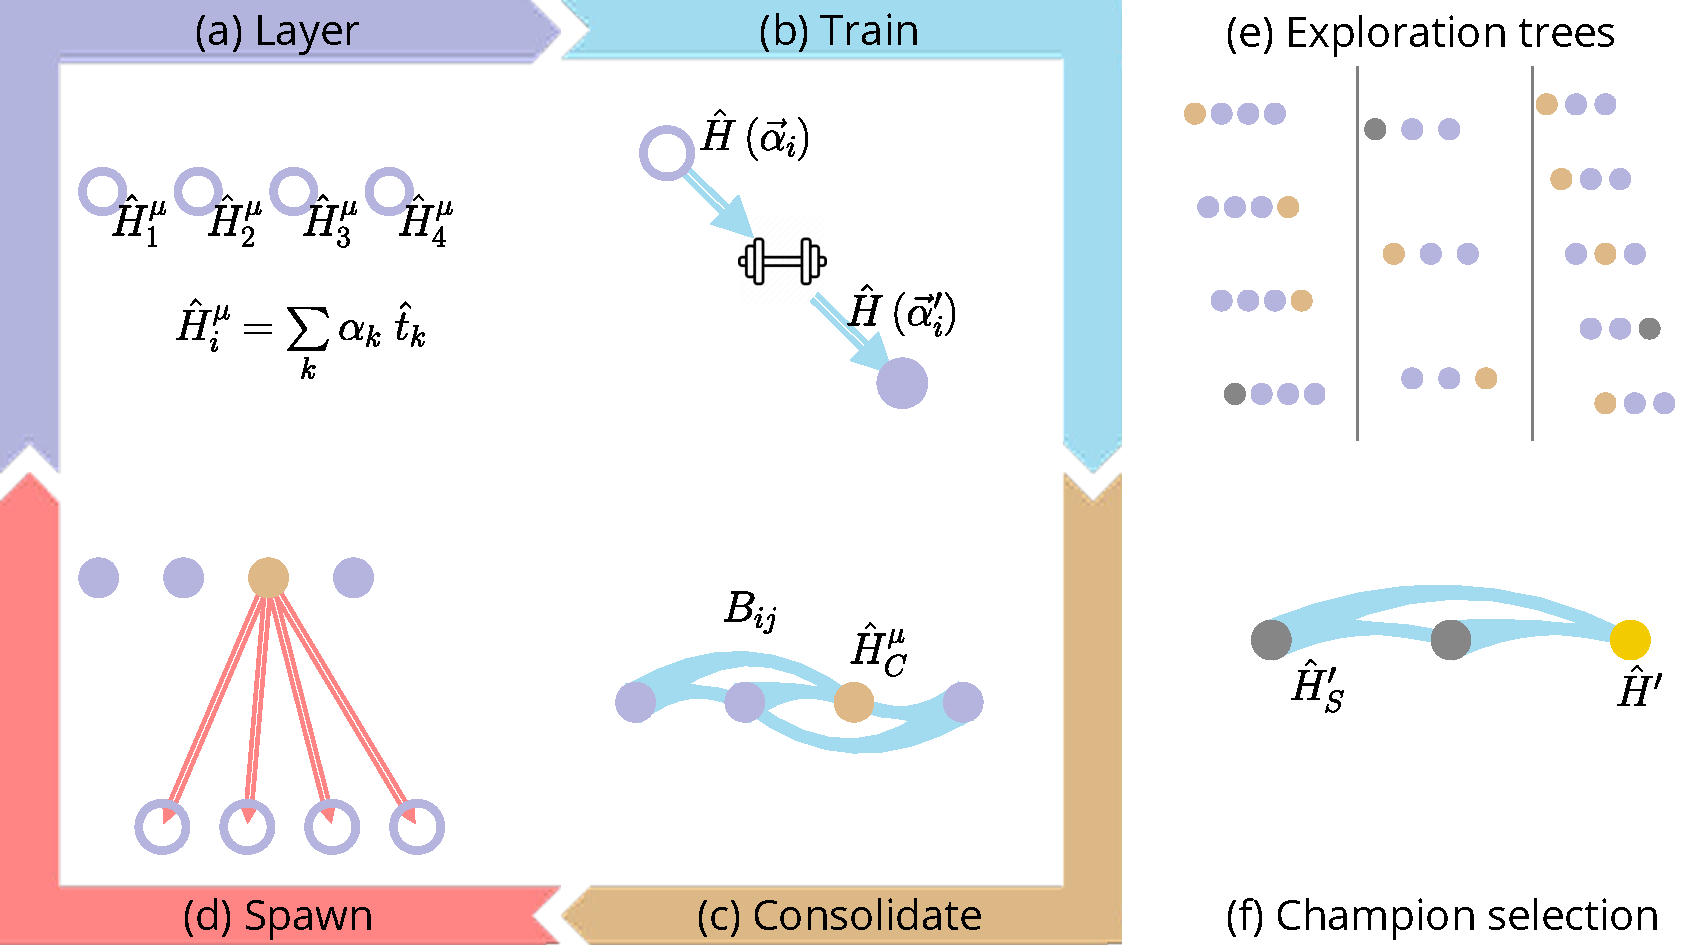
\includegraphics[width=\textwidth]{figure_development/overview_loop.pdf}
    \caption[Quantum Model Learning Agent overview]{
        Schematic of \acrfull{qmla}. 
        \textbf{(a-d)} \gls{ms} phase within an Exploration strategy (ES).
        \textbf{(a)} Models are placed as (empty, purple) nodes on the \emph{active layer} $\mu$, 
            where each model is a sum of terms $\hat{t}_k$ multiplied by a scalar parameter $\alpha_k$. 
        \textbf{(b)} Each active model is trained according to a subroutine such as 
            quantum Hamiltonian learning to optimise $\al_i$, 
            resulting in the trained (filled purple node) $\hat{H}(\al_i^{\prime})$. 
        \textbf{(c)} $\mu$ is consolidated, i.e. models are evaluated relative to other
            models on $\mu$, according to the consolidation mechanism specificed by the \gls{es}.
            In this example, pairwise Bayes factors $B_{ij}$ between $\hi, \hj$ are computed, 
            resulting in the election of a single layer champion $\hat{H}_C^{\mu}$ (bronze). 
        \textbf{(d)} A new set of models are \emph{spawned} according to the chosen
            \gls{es}'s model genertion strategy.
            In this example, models are spawned from a single parent. 
        \textbf{(e-f)} Higher level of entire QMLA procedure.
        \textbf{(e)} The \gls{ms} phase is presented on \emph{exploration trees}. 
            Multiple \gls{es} can operate in parallel, e.g. assuming different underlying physics.
            Each \gls{es} nominates a champion, $\hat{H}_{S}^{\prime}$ (silver), 
            after consolidating its branch champions (bronze). 
        \textbf{(f)} $\hat{H}_{S}^{\prime}$ from each of the above exploration trees are gathered on a single layer, 
            which is consolidated to give the final champion model, $\hp$ (gold). 
    }
    \label{fig:qmla_overview}
\end{figure}

%%%%%%%%%%% EXPLORATION STRATEGIES %%%%%%%%%%% 
\section{Exploration Strategies}\label{sec:exploration_strategies}
\gls{qmla} is implemented by running $\Nt$ \glspl{et} concurrently, 
    where each \gls{et} corresponds to  a unique \gls{ms} and ultimately nominates a single 
    model as its favoured approximation of $\ho$. 
An \gls{es} is the set of rules which guide a single \gls{et} throughout its \gls{ms}. 
We elucidate the responsibilities of \glspl{es} in the remainder of this section, but in short they can be summarised as: 

\begin{easylist}[enumerate]
    \ListProperties(Numbers=r)
    & model generation: 
        combining the knowledge progressively acquired on the \gls{et} to construct new candidate models;
    & decision criteria for the \gls{ms} phase:
        instructions for how \gls{qmla} should respond at predefined junctions, 
        e.g. whether to cease the \gls{ms} after a branch has completed;
    & true model specification:
        detailing the terms and parameters which constitute $\ho$ (in the case where $Q$ is simulated);
    & modular functionality: 
        subroutines called throughout \gls{qmla} are interchangeable such that each \gls{es} specifies the 
        set of functions to achieve its goals.
\end{easylist}
\par 

\gls{qmla} acts in tandem with one or more \glspl{es}, through the process depicted in \cref{fig:qmla_flow}. 
In summary: 
    \gls{qmla} sends a request to the \gls{es} for a set of models; 
    \gls{es} designs models and places them as leaves on one of its branches, and returns the set $\mathbb{H}$; 
    \gls{qmla} places $\mathbb{H}$ on a unique layer; 
    \gls{qmla} trains the models in $\mathbb{H}$; 
    \gls{qmla} consolidates $\mathbb{H}$;
    \gls{qmla} informs the \gls{es} of the results of training/consolidation of $\mathbb{H}$; 
    \gls{es} decides whether to continue the search, and informs \gls{qmla}.
\tikzstyle{startstop} = [
    rectangle, rounded corners, 
    minimum width=12cm, 
    minimum height=2cm,
    % text top, 
    text centered, 
    text width=7cm, 
    text depth=1mm,
    text height=-5mm,
    draw=black, 
    fill=red!30
]
\tikzstyle{io} = [
    trapezium, trapezium left angle=70, trapezium right angle=110, minimum width=3cm,
    minimum height=1cm, text width = 3cm, text centered, draw=black, fill=blue!30
]
\tikzstyle{process} = [
    rectangle, 
    minimum width=5cm, 
    minimum height=2cm, 
    text centered, 
    text width=4.5cm, 
    text depth=3mm,
    text height=-100mm,
    draw=black, 
    fill=orange!30
]

\tikzstyle{decision} = [
    rectangle,
    % trapezium, 
    % trapezium left angle=70, 
    % trapezium right angle=110, 
    minimum width=2cm, 
    minimum height=1cm, 
    text width = 1.8cm, 
    text centered, 
    draw=black, 
    fill=green!30
]
\tikzstyle{decided} = [
    rectangle, 
    minimum width=0.5cm, 
    minimum height=1cm, 
    text centered, 
    text width=1cm, 
    draw=black, 
    fill=blue!30
]
\tikzstyle{qmla_step} = [
    circle, 
    fill=white, 
    draw=red, 
    text=red, 
    minimum size=0.65cm
]

\tikzstyle{arrow} = [thick,->,>=stealth]



\begin{figure}
    \begin{center}
    
    \begin{tikzpicture}[node distance=2.25cm]
    
    \node (qmla) [startstop, label={[shift={(0ex,-5ex)}]north:Quantum Model Learning Agent}] {};
    
    \node (es) [process, below of=qmla, xshift=-1cm, ] {Exploration Strategy};
    
    \node (qhl) [process, below of=es] {Model Trainer};   

    \node (system) [decision, right of=qhl,  xshift=1cm, below of=qhl] {System \gls{q}};   

    \node (simulator) [decision, below of=system, yshift=0.5cm, ] {Simulator};   

    \node (champion) [decided, below of=simulator, yshift=0.5cm, xshift=-1cm, left of=simulator] {$\hat{H}^{\prime}_{S}$};   
 
    \draw [arrow, red] ([yshift=+0.5cm]es.west) -| node[qmla_step]{1}  ([xshift=-4cm]qmla.south);
    \draw [arrow, red] ([xshift=-4.5cm]qmla.south) |- node[qmla_step]{2a}  ([yshift=-0.5cm]es.west);
    \draw [arrow, red] ([yshift=-10pt]es.east)  -| node[qmla_step]{2c}  ([xshift=+62.5pt]qmla.south);
    \draw [arrow, red] ([xshift=-5.1cm]qmla.south) |- node[qmla_step]{4a}  ([yshift=-10pt]qhl.west);
    \draw [arrow, red] ([xshift=+0.5cm]qhl.south) |- node[qmla_step]{4d}  ([yshift=+0pt]system.west);
    \draw [arrow, red] ([xshift=+1.25cm]qhl.south) |- node[qmla_step]{4e}  ([yshift=+0pt]simulator.west);
    \draw [arrow, red] ([yshift=-10pt]qhl.east) -| node[qmla_step]{4g} ([xshift=+2.75cm]qmla.south) ;
    \draw [arrow, red] ([xshift=+5.5cm]qmla.south) |- node[qmla_step]{7}  ([yshift=+0pt]champion.east);
    
    % \node (step_4) [qmla_step, left of=(0.1cm of qmla), above=(0.1cm of qmla.south)]{4};
    \node (step_3) [qmla_step, left of=qmla.west, xshift=0cm, above=(0.1cm of qmla.south)]{3};
    \node (step_5) [qmla_step, right of=step_3, xshift=3.75cm, ]{5};
    \node (step_6) [qmla_step, right of=step_5, xshift=-1cm,]{6};
    % \node (step_6a) [qmla_step, right of=step_6, xshift=-1cm]{6a};

    \node (step_2b) [qmla_step, above=(0.1cm of es.south)]{2b};

    \node (step_4b) [qmla_step, right of=qhl.west, xshift=-4cm, above=(0.1cm of qhl.south)]{4b};
    \node (step_4c) [qmla_step, right of=step_4b, xshift=-1cm]{4c};
    \node (step_4f) [qmla_step, right of=step_4c, ]{4f};


    \end{tikzpicture}
    \end{center}
    
    \caption[Interface between \glsentryshort{qmla} and a single \glsentrylong{es}]{
        Interface between \glsentryfull{qmla} and a single \glsentryfull{es}
        The main components are the \gls{es}, model training subroutine, target quantum system (i.e. black box, \gls{q}), 
        and (quantum) simulator. 
        The main steps of the algorithm, shown in red with arrows denoting data transferred during that step, are as follows.
        \textbf{1}, QMLA retrieves decision infrastructure from ES, such as the consolidation mechanism and termination criteria.
        \textbf{2}, models are designed/spawned; 
        \textbf{2a}, QMLA signals to ES requesting a set of models, passing the results of the previous layers' models if appropriate.
        \textbf{2b}, ES spawns new models, $\mathbb{H}$;
        \textbf{2c}, ES passes $\mathbb{H}$ to QMLA. 
        \textbf{3}, QMLA assigns a new layer $(\mu \gets \mu + 1)$ and places the newly proposed models upon it.
        \textbf{4}, Model training subroutine (here quantum Hamiltonian learning), performed independently for each model $\hi \in \mu$; 
        \textbf{4a}, QMLA passes $\hi$ to the model trainer; 
        \textbf{4b}, construct a prior distribution $P_i$ describing the model's parameterisation $\vec{\alpha}_i$;
        \textbf{4c}, design experiment $e$ to perform on \gls{q} to optimise $\vec{\alpha}_i$;
        \textbf{4d}, perform $e$ on \gls{q} to retrieve a datum $d$;
        \textbf{4e}, simulate $e$ for particles $\{ \vec{\alpha}_1, \dots , \vec{\alpha}_N \}$ 
            sampled from $P_i$ to retrieve a \emph{likelihood} $\lk_{e}$;
        \textbf{4e}, update the prior $P_i$ based on $(d, \lk_{e})$.
        \textbf{5}, Evaluate and rank $\hi \in \mu$ according to the ES's consolidation mechanism.
        \textbf{6}, Check ES's termination criteria; if reached, proceed to \textbf{(7)}, otherwise return to \textbf{(2)}.
        \textbf{7}, Nominate \gls{champion model}, $\hp_{S}$.        
    }
    \label{fig:qmla_flow}
\end{figure}

   

\subsection{Model generation}\label{sec:model_generation}
The main role of any \gls{es} is to design candidate models to test against $\ho$. 
This can be done through any means deemed appropriate, 
    although in general it is sensible to exploit the information gleaned so far in the \gls{et}, 
    such as the performance of previous candidates and their comparisons, 
    so that successfel models are seen to \emph{\gls{spawn}} new models, 
    e.g. by combining previously successful models, or by building upon them. 
Conversely, model generation can be completely determined in advance or entirely random.
This alludes to the central design choice in composing an \gls{es}: 
    how broad and deep should the searchable \emph{model space} be, 
    considering that adequately training each model
    is expensive, and that model comparisons are similarly expensive. 
The \gls{ms} occurs within some \emph{\gls{model space}}, the size of which can usually be easily found 
    by assuming that terms are binary -- either the interaction they represent is present or not. 
If all possible terms are accounted for, and the total set of terms is $\termset$,
    then there are $2^\absval{\termset}$ available candidates in the model space. 
The model space encompasses the closed\footnotemark set of models construable by the set of terms considered by an \gls{es}. 
Because training models is slow in general,
    a central aim of \gls{qmla} is to search this space efficiently,
    i.e. to minimise the number of models considered, while retaining high quality models and 
    providing a reasonable prospect of uncovering the true model, or a strong approximation thereof. 

\footnotetext{
    It is feasible to define an \gls{es} which uses an open model space, that is, there is no pre-defined $\termset$, 
    but rather the \gls{es} determines models through some other heuristic mechanism. 
    In this thesis, we do not propose any such \gls{es}, but note that the \gls{qmla} framework 
    facilitates the concept, see \cref{chapter:sw}.   
}



\subsection{Decision criteria for the model search phase}
Further control parameters, which direct the growth of the \gls{et}, are set within the \gls{es}.
At several junctions within Algs. \ref{alg:qmla}, \ref{alg:model_search}, 
    \gls{qmla} queries the \gls{es} in order to decide what happens next.
Here we list the important cases of this behaviour. 

\begin{easylist}[enumerate]
    % \ListProperties(Numbers=r, Start=1)
    \ListProperties(Numbers=r)
    & Parameter-learning settings
    && such as the prior distribution to assign each parameter during \gls{qhl}, and the parameters needed to run \gls{smc}.
    && the time scale on which to examine $Q$.
    && the input probes to train upon. 
    & Branch comparison strategy
    && How to compare models within a branch (or \gls{qmla} layer). 
        Some examples used in this work are
        (a) a points-ranking where each points are assigned according to Eqn. \ref{eqn:bf_cases}
        (b) ranking reflecting each model's log-likelihood after training. 
        All methods in \S\ref{sm:objective_fncs} can be thought of as branch comparison strategies. 
    & \gls{ms} termination criteria
    && e.g. instruction to stop after a fixed number of iterations, or when a certain fitness has been reached.
    & Champion nomination
    && when a single tree is explored, identify a single champion from the branch champions
    && if multiple trees are explored, how to compare champions across trees. 
\end{easylist}

\subsection{True model specification}
It is necessary also to specify details about the true model $\ho$, 
    at least in the case where \gls{qmla} acts on simulated data. 
Within the \gls{es}, we can set $\terms_0$ as well as $\al_0$. 
For example where the target system is an untrusted quantum simulator to be characterised, 
    $S_u$, by interfacing with a trusted (quantum) simulator $S_t$, 
    we decide some $\ho$ in advance:
    the model training subroutine calls for \glspl{likelihood}, 
    those corresponding to $\ho$ are computed $S_u$, 
    while particles' \gls{likelihood} are computed on $S_t$. 

\subsection{Modular functionality}
Finally, there are a number of fundamenetal subroutines which are called upon throughout the \gls{qmla} algorithm. 
These are written independently such that each subroutine has a number of available implementations. 
These can be chosen to match the requirements of the user, and are set via the \gls{es}. 

\begin{easylist}[enumerate]
    % \ListProperties(Numbers=r, Numbers2=l,Start=1,)
    \ListProperties(Numbers=r, Numbers2=l,)
    & Model training procedure
    && i.e. whether to use \gls{qhl} or quantum process tomography, etc. 
    && In this work we always used \gls{qhl}. 
    & Likelihood function: the method used to estimate the likelihood 
        for use during quantum likelihood estimation within \gls{qhl}, 
        which ultimately depends on the measurement scheme. 
    && By default, here we use projective measurement back onto the input probe state, 
        $\left| \bra{\psi} e^{-i\hat{H}t} \ket{\psi} \right|^2$.
    && It is possible to change this to implement any measurement procedure, 
        for example an experimental procedure where the environment is traced out. 
    & \label{item:probes} Probes: defining the input probes to be used during training. 
        && In general it is preferable to use numerous probes in order to avoid biasing particular terms. 
        && In some cases we are restricted to a small number available input probes, e.g. to match experimental constraints.
    & Experiment design heuristic: bespoke experiments to maximise the information 
        on which models are individually trained.
        && In particular, in this work the experimental controls consist solely of $\{ \ket{\psi}, t \}$. 
        && Currently, probes are generated once according to \ref{item:probes}, 
            but in principle it is feasible to choose optimal probes based on available or hypothetical information. 
            For example, probes can be chosen as a normalised sum of the candidate model's eigenvectors.
        && Choice of $t$ has a large effect on how well the model can train. 
            By default times are chosen proportional to the inverse of the 
            current uncertainty in $\al$ to maximise Fischer information, 
            through the multi-particle guess heuristic \cite{Wiebe:2014qhl}.
            Alternatively, times may be chosen from a fixed set to force \gls{qhl} to 
            reproduce the dynamics within those times' scale. 
            For instance, if a small amount of experimental data is available offline, 
            it is sensible to train all candidate models against the entire dataset.  
    & Model training prior: change the prior distribution, e.g. Fig. \ref{fig:qhl_smc}(a)
\end{easylist}

\subsection{Exploration strategy examples}
To solidifiy the concept of \glspl{es}, and how they affect the overall,
    reach and runtime of a given \gls{et}, consider the following examples, 
    where each strategy specifies how models are generated, as well as how trained models are compared within a branch. 
Recall that all of these strategies rely on \gls{qhl} as the model training strategy, 
    so that the run time for training, is $t_{\textrm{QHL} \sim \Ne\Np t_U}$, 
    where $t_U(n)$ is the time to compute the unitary evolution via the matrix exponential for an $n$-qubit model 
All models are trained using the default \gls{likelihood} in \cref{eqn:likelihood}. 
Assume the conditions
\begin{easylist}[itemize]
    & all models considered are represented by 4-qubit models;
    && $t_{U(4)} \sim 10^{-3}\textrm{sec}$. 
    & each model undergoes a reasonable training regime;
    && $\Ne=1000, \Np=3000$;
    && $\implies t_{\textrm{QHL}} = \Ne \times \Np \times  t_{U(4)} = 3000s \sim 1 \textrm{h} $;
    & Bayes factor calculations use 
    && $\Ne=500, \Np=3000 $
    && $\implies t_{\textrm{BF}} \sim 2 \times  500 \times 3000 \times  10^{-3} \sim 1 \textrm{h}$;
    & there are 12 available terms
    && allowing any combination of terms, this admits a model space of size $2^{12} = 4096$
    & access to 16 computer cores to parallelise calculations over
    && i.e. we can train 16 models or perform 16 \gls{bf} comparisons in $1h$.
\end{easylist}
\par 

\noindent Then, consider the following model generation/comparison strategies.
\begin{easylist}[enumerate]
    \ListProperties(Numbers1=l, Numbers2=r)
    & \label{gr:predefined} Predefined set of $16$ models, comparing every pair of models
    && Training takes $1h$, and ${16 \choose 2} = 120$ comparisons need $8h$
    && total time is $9h$. 
    & \label{gr:generative_full} Generative procedure for model design, comparing every pair of models,
        running for 12 branches
    && One branch takes $9h \implies$ total time is $12 \times 9 = 108h$; 
    && total number of models considered is $16 \times 12 = 192$. 
    & \label{gr:generative_sparse} Generative procedure for model design, where less model comparisons are needed 
        (say one third of all model pairs are compared),
        running for 12 branches
    && Training time is still $1h$
    && One third of comparisons, i.e. $40$ \gls{bf} to compute, requires $3h$
    && One branch takes $4 h \implies$ total time is $36 h$
    && total number of models considered is also $192$. 
\end{easylist}

These examples illustrate some of the design decisions involved in \gls{es}s, 
    namely whether timing considerations are more important than thoroughly exploring the model space.
They also show considerable time--savings in cases where it is
    acceptable to forego all model comparisons. 
The approch in \ref{gr:predefined} is clearly limited in its applicability, 
    mainly in that there is a heavy requirement for prior knowledge, 
    and it is only useful in cases where we either know $\ho \in \mathbb{H}$, 
    or would be satisfied with approximating $\ho$ as the closest available $\hj \in \mathbb{H}$. 
On the opposite end of this spectrum, \ref{gr:generative_sparse}  is an excellent approach
    with respect to minimising prior knowledge required by the algorithm, 
    although at the significant expense of testing a much larger number of candidate models. 
There is no optimal strategy for all use--cases: 
    specific quantum systems of study demand particular considerations, 
    and the amount of prior information available informs how wide the model search should reach. 

\par 

In this work we have used two straightforward model generation routines.
Firstly, during the study of various physical classes (Ising, Heisenberg, Fermi-Hubbard), 
    a list of lattice configurations were chosen in advance,
    which were then mapped to Hamiltonian models.
This \gls{es} is non-adaptive and indeed the model search
    consists merely of a single branch with no subsequent calls to the model generation routine, 
    as in \ref{gr:predefined}. 
In the latter section instead we use a \gls{ga}:
    this is clearly a far more general strategy, at a significant computational cost, 
    but is suitable for systems where we have less knowledge in advance. 
In this case, new models are designed based heavily on results from earlier branches of the \gls{et}. 
The genetic algorithm model generation subroutine is listed in Alg. \ref{alg:generate_models}, 
    and can broadly be summed up thus: 
    the best models in a generation $\mu$ produce offspring which constitute models on the next generation.
These types of evolutionary algorithms ensure that newly proposed candidates inherit 
    some of the structure which rendered previous candidates (relatively) successful, 
    in the expectation that this will yield ever-stronger candidates. 

%%%%%%%%%%% GENERALITY %%%%%%%%%%% 

\section{Generality}
Several aspects of \gls{qmla} are deliberately vague in order to facilitate generality. 
\begin{easylist}[itemize]
    & \emph{Model} can mean any description of a quantum system which captures the interactions it is subject to. 
    && Here we exclusively consider Hamiltonian models, but Lindbladian models can also be considered as generators of quantum dynamics. 
    & \emph{Model training} is any subroutine which can train a given model, i.e. optimise a given parameterisation 
        under the assumption that represents the target system. 
    && Currently only \gls{qhl} has been used, but tomography is valid in principle, albeit slower. 
    && \Gls{qhl} relies on the calculation of a characteristic \gls{likelihood} function; 
        this too is not restricted to the generic form of \cref{eqn:likelihood} and can be replaced by 
        any form which represents the likelihood that experimental conditions $e$ result in measurement datum $d$. 
        We will see examples of this in \cref{chapter:nv} where we trace out part of the system in order 
        to represent open systems. 
    & \emph{Model selection}, or \emph{consoldation} can be as rigourous as desired by the user. 
    && Consolidation occurs at the branch level of each \gls{et}, but also in finding the tree champion, 
        and ultimately the global champion. 
    && In practice, we use either \gls{bf} or a related concept such as \gls{tltl} which are statistically signicative. 
        However, in \cref{sec:ga} we will consider a number of alternative schemes for discerning the strongest models. 
    

\end{easylist}

\subsection{Agency}
While the concept of \emph{agency} is contentious \cite{franklin1996agent}, 
    we can view our overall protocol as a multi-agent system \cite{wooldridge2009introduction}, 
    or even an agent based evolutionary algorithm \cite{sarker2010agent}, 
    because any given \gls{es} satisfies the definition,
    \emph{the  population  of  individuals can be considered as a population of agents}, 
    where we mean the population of models present on a given \gls{et}. 
More precisely, we can view individual models as \emph{learning agents} according to the criteria of 
    \cite{russell2002artificial}, i.e. that a learning agent has
    \begin{easylist}[itemize]
        & a \emph{problem generator}: designs actions in an attempt to learn about the system -- this is precisely the role of the \gls{edh};
        & a \emph{performance element}: implements the the designed actions and measures the outcome
            -- the measurement of a datum following the experiment chosen by the \gls{edh}; 
        & a \emph{critic}: the likleihood function informs whether the designed action (experiment) was successful; 
        & a \emph{learning element}: the updates to the weights and overall parameter distribution improve the model's performance over time. 
    \end{easylist}
We depict this analogy in \cref{fig:learning_agent}.
Finally, the model design strategy encoded in the \gls{es} \emph{can} allow agency,
    by permitting the spawn rules autonomy, 
    so we label the entire procedure as the quantum model learning agent. 

\tikzstyle{startstop} = [
    rectangle, rounded corners, 
    minimum width=12cm, 
    minimum height=2cm,
    % text top, 
    text centered, 
    text width=7cm, 
    text depth=1mm,
    text height=-5mm,
    draw=black, 
    fill=red!30
]
\tikzstyle{io} = [
    trapezium, trapezium left angle=70, trapezium right angle=110, minimum width=3cm,
    minimum height=1cm, text width = 3cm, text centered, draw=black, fill=blue!30
]

\tikzstyle{environment} = [
    rectangle, rounded corners, 
    minimum width=3cm, 
    minimum height=8.5cm,
    % text top, 
    text centered, 
    % text width=1.5cm, 
    % text depth=1mm,
    % text height=-5mm,
    draw=black, 
    fill=red!30
]
\tikzstyle{process} = [
    rectangle, 
    minimum width=3cm, 
    minimum height=1.5cm, 
    text centered, 
    text width=2cm, 
    draw=black, 
    fill=orange!30
]

\tikzstyle{decision} = [
    rectangle,
    % trapezium, 
    % trapezium left angle=70, 
    % trapezium right angle=110, 
    minimum width=2cm, 
    minimum height=1cm, 
    text width = 1.8cm, 
    text centered, 
    draw=black, 
    fill=green!30
]
\tikzstyle{decided} = [
    rectangle, 
    minimum width=0.5cm, 
    minimum height=1cm, 
    text centered, 
    text width=1cm, 
    draw=black, 
    fill=blue!30
]
\tikzstyle{agent_step} = [
    circle, 
    % fill=white, 
    % draw=red, 
    text=red, 
    minimum size=0.65cm
]

\tikzstyle{arrow} = [thick,->,>=stealth]


\usetikzlibrary{calc}
\tikzset{>=latex}
\tikzstyle{a}=[fill=red,circle,inner sep=2pt]
\tikzstyle{b}=[fill=blue,circle,inner sep=2pt]

% \begin{tikzpicture}
%   \node [a] (A) at (0,0) {};
%   \node [b] (B) at (4,0.8) {};

%   \coordinate (A2) at ($ (A) - (0,1) $);
%   \coordinate (B2) at ($ (B) - (0,1) $);
%   \coordinate (B3) at ($ (B)!(A2)!(B2) $);

%   \draw [<->,very thick] (A2) -- (B3);
% \end{tikzpicture}


\begin{figure}
    \centering
    \begin{minipage}[c]{0.4\textwidth}
    
        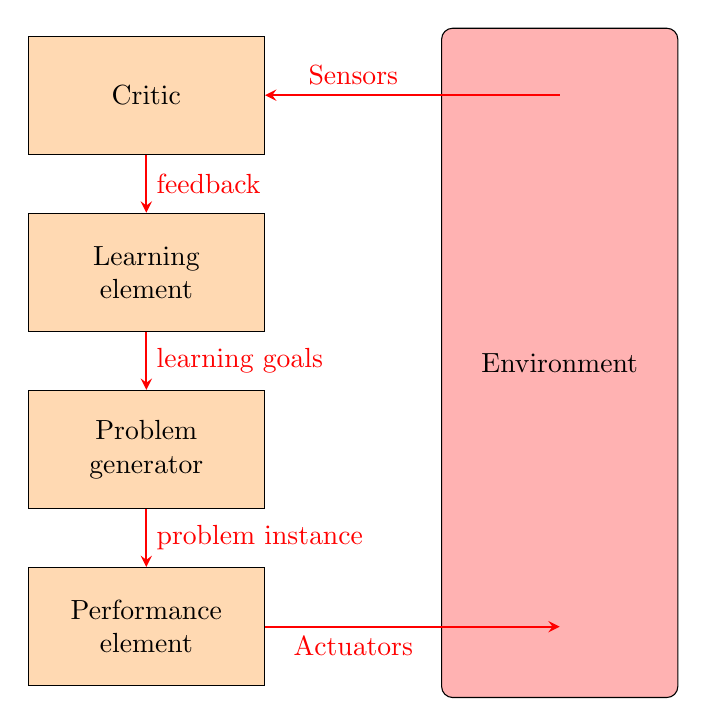
\begin{tikzpicture}[node distance=2.25cm]
        
        \node (critic) [ process] {Critic};
        \node (learning_element) [process, below of=critic] {Learning element};   
        \node (problem_generator) [process, below of=learning_element,] {Problem generator};   
        \node (performance_element) [process, below of=problem_generator,] {Performance element};   
        \node (environment) [environment, right of=critic, xshift=3cm, yshift=-3.4cm] {Environment};   
    
        \coordinate (B1) at ($ (environment) + (0,1)$);
        \coordinate (B2) at ($ (environment) - (0,1)$);
        \coordinate (perf_env) at ($ (environment)!(performance_element.east)!(B2) $);
        \coordinate (env_critic) at ($ (environment)!(critic.east)!(B1) $);

        \draw [arrow, red] (critic.south) -- node[anchor=west]{feedback} (learning_element.north);
        \draw [arrow, red] (learning_element.south) -- node[anchor=west, ]{learning goals} (problem_generator.north);
        \draw [arrow, red] (problem_generator.south) -- node[anchor=west, ]{problem instance} (performance_element.north);
        \draw [arrow, red] (performance_element.east) -- node[anchor=north, xshift=-0.75cm]{Actuators} (perf_env);
        \draw [arrow, red] (env_critic) -- node[anchor=south,xshift=-0.75cm]{Sensors} (critic.east);
        
        \end{tikzpicture}
    \end{minipage}
    ~\hspace{2cm}
    \begin{minipage}[c]{0.4\textwidth}
    
        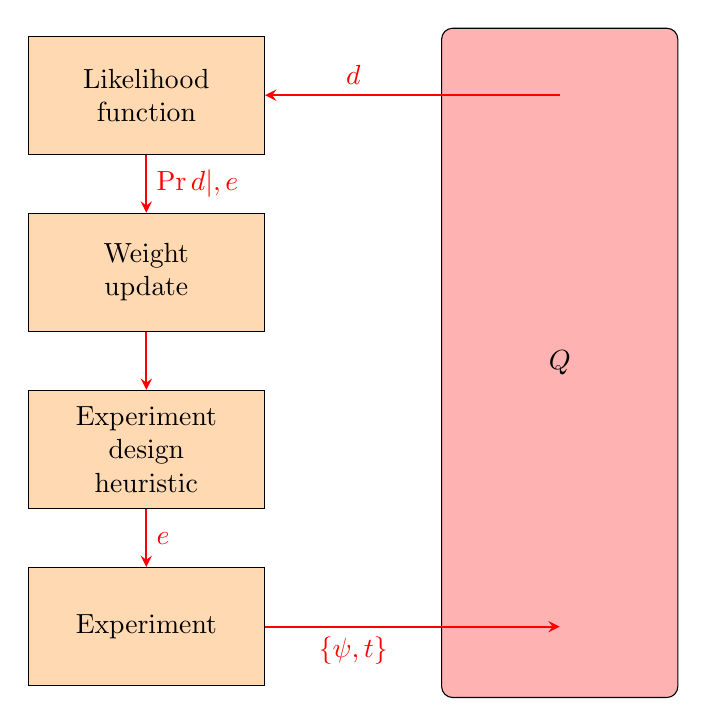
\begin{tikzpicture}[node distance=2.25cm]
        
        \node (critic) [ process] {Likelihood function};
        \node (learning_element) [process, below of=critic] {Weight update};   
        \node (problem_generator) [process, below of=learning_element,] {Experiment design heuristic};   
        \node (performance_element) [process, below of=problem_generator,] {Experiment};   
        \node (environment) [environment, right of=critic, xshift=3cm, yshift=-3.4cm] {$Q$ };   
    
        \coordinate (B1) at ($ (environment) + (0,1)$);
        \coordinate (B2) at ($ (environment) - (0,1)$);
        \coordinate (perf_env) at ($ (environment)!(performance_element.east)!(B2) $);
        \coordinate (env_critic) at ($ (environment)!(critic.east)!(B1) $);

        \draw [arrow, red] (critic.south) -- node[anchor=west]{$\Pr\bk{d | \al, e}$} (learning_element.north);
        \draw [arrow, red] (learning_element.south) -- node[anchor=west, ]{$\pra$} (problem_generator.north);
        \draw [arrow, red] (problem_generator.south) -- node[anchor=west, ]{$e$} (performance_element.north);
        \draw [arrow, red] (performance_element.east) -- node[anchor=north, xshift=-0.75cm]{$\{ \ket{\psi}, t \}$} (perf_env);
        \draw [arrow, red] (env_critic) -- node[anchor=south,xshift=-0.75cm]{$d$} (critic.east);
        
        \end{tikzpicture}
    \end{minipage}


    \caption[Learning agents]{
        Learning agents. \textbf{Left}: definition of a learning agent, where an \emph{environment} is affected by 
        \emph{actuators} which realise a \emph{problem instance}, designed by a \emph{problem generator}, through some \emph{performance element}. 
        The result of the agent's action is detected by \emph{sensors}, which the \emph{critic} interprets with respect to
        the agent's \emph{learning goals}, by providing \emph{feedback} to the \emph{learning element}. 
        \emph{Right}: mapping of the concept of a learning agent on to an individual model. 
        A target quantum system, $Q$, is queried by performing some experiment $e$, 
        designed by an experiment design heuristic, and implemented by evolving a probe state $\ket{\psi}$ for time $t$. 
        The systems is measured, and the datum $d$ is sent to the \gls{likelihood} function, which sends the likelihood $\Pr(d|\al, t)$
        to the weight update (and the parameter distribution update), before designing another experiment. 
    }
    \label{fig:learning_agent}
\end{figure}

   


%%%%%%%%%%% PSEUDOCODE %%%%%%%%%%% 
\section{Algorithms}
We conclude this chapter by listing the algorithms used most frequently, 
    in order to clarify each of their roles, and how they interact. 
Alg \ref{alg:qmla} shows the overall \gls{qmla} algorithm, 
    which is simplified greatly to a loop over the \gls{ms} of each \gls{es}. 
The \gls{ms} iteself is listed in Alg. \ref{alg:model_search},
    which contains calls to subroutines for model learning (\gls{qhl}, Alg. \ref{alg:qhl}), 
    branch evaluation (which can be based upon \gls{bf}, Alg. \ref{alg:bayes_factor})
    and centers on the generation of new models, an example of which -- based on a genetic algorithm -- 
    is given in  Alg. \ref{alg:generate_models}. 

\begin{algorithm}
    \caption{Quantum Model Learning Agent}
    \label{alg:qmla}
    \DontPrintSemicolon
    \KwIn{ $Q$ \tcp*[1]{some physically measurable or simulateable quantum system}}
    \KwIn{ $\mathbb{S}$ \tcp*[1]{set of exploration strategies}}\;

    \KwOut{$\hat{H}^{\prime}$ \tcp*[1]{champion model}}\;
    
    $\mathbb{H}_c \gets \{\}$\;   
    \For{$S \in \mathbb{S}$ }{
        $\hat{H}_{S}^{\prime} \gets$ \ttt{model\_search(Q, S)} 

        $\mathbb{H}_c \gets \mathbb{H}_c \cup  \{\hat{H}_{S}^{\prime}\}$ \tcp*[1]{add ES champion to collection}
    }
    $\hat{H}^{\prime} \gets $ \ttt{final\_champion($\mathbb{H}_c$)}\;
    return $\hat{H}^{\prime}$

\end{algorithm}

\begin{algorithm}
    \caption{ES subroutine: \ttt{model\_search}}
    \label{alg:model_search}
    \DontPrintSemicolon
    \KwIn{ $Q$ \tcp*[1]{some physically measurable or simulateable quantum system}}
    \KwIn{ $S$ \tcp*[1]{Exploration strategy: collection of rules/subroutines}}\;

    \KwOut{$\hat{H}_{S}^{\prime}$ \tcp*[1]{Exploration strategy's nominated champion model}}\;
     
    $\nu \gets \{\}$

    $\mathbb{H}_c \gets \{\}$\;   
    \While{ \ttt{!S.terminate()} }{
        $\mu \gets $ \ttt{S.generate\_models($\nu$)} \tcp*[1]{e.g. Alg. \ref{alg:generate_models}}\; 

        \For{ $\hi \in \mu$}{
            $\hi^{\prime} \gets $ \ttt{S.train($\hi$)} \tcp*[1]{e.g. Alg. \ref{alg:qhl}}
        }
        $\nu \gets$ \ttt{S.evaluate($\mu$)} \tcp*[1]{e.g. pairwise via Alg. \ref{alg:bayes_factor}}

        $\hat{H}_{c}^{\mu} \gets $ \ttt{S.branch\_champion($\nu$)} \tcp*[1]{use $\nu$ to select a branch champion}

        $\mathbb{H}_c \gets \mathbb{H}_c \cup \{\hat{H}_c^{\mu}\}$ \tcp*[1]{add branch champion to collection}
    }

    $\hat{H}_{S}^{\prime} \gets $ \ttt{S.nominate\_champion($\mathbb{H}_c$)}\;
    return $\hat{H}_{S}^{\prime}$

\end{algorithm}


\begin{algorithm}
    \caption{ES subroutine: \ttt{generate\_models} (example: genetic algorithm)}
    \label{alg:generate_models}
    \DontPrintSemicolon
    \KwIn{ $\nu$ \tcp*[1]{information about models considered to date}}\;
    \KwIn{ $g(\hi)$ \tcp*[1]{objective function}}\;

    \KwOut{$\mathbb{H}$ \tcp*[1]{set of models}}\;
    
    $ N_m = \left| \nu \right| $ \tcp*[1]{number of models}

    \For{$\hi \in \nu$}{
       $g_i \gets g(\hi)$ \tcp*[1]{model fitness via objective function}
    }
    $r \gets $ \ttt{rank($\{ g_i \}$)} \tcp*[1]{rank models by their fitness}
    $\mathbb{H}_t \gets $ \ttt{truncate($r, \frac{N_m}{2}$)} \tcp*[1]{truncate models by rank: only keep $\frac{N_m}{2}$}
    $ s \gets $ \ttt{normalise($\{g_i\}$)} $\forall \hi \in \mathbb{H}_t$ \tcp*[1]{normalise remaining models' fitness}

    $\mathbb{H} = \{\}$ \tcp*[1]{new batch of chromosomes/models}

    \While{ $\left| \mathbb{H} \right| < N_m$ }{
        $p_1, p_2 = $ \ttt{roulette($s$)} \tcp*[1]{use $s$ to select two parents via roulette selection}
    
        $c_1, c_2$ = \ttt{crossover($p_1, p_2$)} \tcp*[1]{produce offspring models}

        $c_1, c_2$ = \ttt{mutate($c_1, c_2$)} \tcp*[1]{probabilistically mutate}

        $\mathbb{H} \gets \mathbb{H} \cup \{ c_1, c_2 \} $ \tcp*[1]{add new models to batch}

    }

    % \ttt{roulette($s$)}

    return $\mathbb{H}$ 

\end{algorithm}



\begin{algorithm}
    \caption{Quantum Hamiltonian Learning}
    \label{alg:qhl}
    \DontPrintSemicolon
    \KwIn{ $Q$ \tcp*[1]{some physically measurable or simulatable quantum system, described by $\ho$}}

    \KwIn{$\hat{H}_i$ \tcp*[1]{Hamiltonian model attempting to reproduce data from $\hat{H}_0$ }}
    \KwIn{$\pra$ \tcp*[1]{probability distribution for $\al = \al_0 $}}
    \KwIn{$\Ne$ \tcp*[1]{number of epochs to iterate learning procedure for}}
    \KwIn{$\Np$ \tcp*[1]{number of particles to draw from $\pra$}}
    \KwIn{\ttt{$\Lambda(\pra)$} \tcp*[1]{Heuristic algorithm which designs experiments}}
    \KwIn{\ttt{RS($\pra$)} \tcp*[1]{Resampling algorithm for redrawing particles}}

    \KwOut{$\al^{\prime}$ \tcp*[1]{estimate of Hamiltonian parameters}}\;


    Sample $\Np$ times from $\pra \gets \mathcal{P}$ \tcp*[1]{particles}\;
    
    \For{$ e \in  \{1 \rightarrow \Ne\}$ }{ 
        
        $t, \ket{\psi} \gets \Lambda(\pra)$ \tcp*[1]{design an experiment}
        
        \For{
            $p \in \mathcal{P}$ 
        }{
            Retrieve particle $p \gets \al_p$
            
            Prepare $Q$ in $\ket{\psi}$, evolve and measure after $t \gets d$ \tcp*[1]{datum}
            
            $| \bra{d} e^{-iH(\al_p)t} \ket{\psi} |^2 \gets Pr(d|\al_p; t)$ \tcp*[1]{likelihood}
                        
            $w_p \gets w_p \times Pr(d|\al_p; t)$ \tcp*[1]{weight update}
        }
        \If{
            $ 1 / \sum_p w_p^2 < \Np/2$
            \tcp*[1]{check whether to resample (are weights too small?)}
        }{
            $\ttt{RS}(\pra) \gets \mathcal{P}$
            \tcp*[1]{Redraw particles via resampling algorithm}
        }
    }
    
    \ttt{mean}($\pra) \gets \vec{\alpha}^{\prime}$\;
    
    return $\al^{\prime}$
     
\end{algorithm}



\begin{algorithm}
    \caption{Bayes Factor calculation}
    \label{alg:bayes_factor}
    \DontPrintSemicolon
    \KwIn{ $Q$ \tcp*[1]{some physically measurable or simulateable quantum system.}}
    \KwIn{ $\hat{H}_j^{\prime}, \hat{H}_k^{\prime}$ \tcp*[1]{Hamiltonian models after QHL (i.e. $\al_j, \al_k$ already optimised), on which to compare performance.}}
    \KwIn{ $\expset_j, \expset_k$ \tcp*[1]{experiments on which $\hat{H}_j^{\prime}$ and $\hat{H}_k^{\prime}$ were trained during QHL.}}
    
    \KwOut{$B_{jk}$ \tcp*[1]{Bayes factor between two candidate Hamiltonians}}
     
     
    $\expset = \{ \expset_j \cup \expset_k \}$ \;
    \For{$\hat{H}_i^{\prime} \in  \{\hat{H}_j^{\prime}, \hat{H}_k^{\prime}$ \} }{
        $\tll_{i} = 0$ \tcp*[1]{total log-likelihood of $\hat{H}_i$} 
        \For{$e \in \expset$}{
            $e \gets t, \ket{\psi}$ \tcp*[1]{assign time and probe from experiment control set}\;

            Prepare $Q$ in $\ket{\psi}$, evolve and measure after $t \gets d$ \tcp*[1]{datum}\;

            $ \absval{ \bra{d} e^{-i \hat{H}_i^{\prime} t} \ket{\psi} }^2 \gets Pr(d | \hat{H}_i, t)$  \tcp*[1]{total likelihood for $\hat{H}_i^{\prime}$ on $e$}\;

            $log \left( Pr(d | \hat{H}_i, t) \right) \gets l_e$ \tcp*[1]{log total likelihood for $\hat{H}_i^{\prime}$ on $e$}\;

            $\tll_{i}+ l_e \gets  \tll_{i}$ \tcp*[1]{add $l_e$ to total log total likelihood }
        }
    }
    
    $\exp\left( \tll_{j} - L_k \right) \gets B_{jk}$  \tcp*[1]{Bayes factor between models}\;
    return $B_{jk}$
\end{algorithm}



    \chapter{Software}\label{chapter:sw}
        All of the details in \cref{chapter:qhl} and \cref{chapter:qmla} are implemented in the \gls{qmla}
    software framework, a (mostly) Python codebase which underlies all of the 
    arguments, results and figures in this thesis. 
The codebase is designed to simplify the process of running \gls{qmla} or \gls{qhl}
    on novel systems.
In particular, the core \gls{qmla} algorithm can support a wide range of \glspl{es}, 
    allowing for the design of bespoke \glspl{es} to account for the specific requirements 
    of any given system. 
In this chapter we give an overview of the \gls{qmla} software, 
    implementation and instructions for its use. 

\section{Implementation}
In this section we describe the technical details of the implementation of the 
    algorithm described in \cref{chapter:qmla}, as well as a number of relevant subroutines. 
We do not introduce new mathematical, physical or algorithmic concepts, 
    so readers interested in applications of the techniques may prefer to skip to \cref{part:theoretical_study}.

\subsection{Object oriented programming}
We first introduce the concepts of object-oriented programming, 
    and in particular \emph{inheritance} between objects, 
    since this will feature in later discussion about the implementation of \gls{qmla}
    and \glspl{es}. 
Python is a robust object-oriented language \cite{python-manual}, meaning that we can frame 
    concepts as objects which permit actions to be performed by/to them. 
In particular, objects in Python are formulated as \emph{classes}, 
    which can have associated \emph{attributes} and \emph{methods}. 
For example, we can encode the concept of a footballer as an object,
    such that the player object has attributes, e.g. number of games played and goals scored in a season, 
    as well as methods for specific calculations, 
    e.g. to summarise their record.
We can then utilise the footballer class to store information about an \emph{individual} player, 
    by making an instance of the class.
\par 

A fundamental concept in object-oriented programming is \emph{inheritance} between objects, 
    such that a \emph{child} objects inherit properties of its \emph{parent}.
In general, a parent object can be thought of as an abstract concept, 
    which provides basic functionality and reasonable default properties,
    while a child object can specify further details. 
For example, an Athlete class can act as a parent to the footballer class, 
    where the Athlete class holds core information such as date of birth. 
This allows for the Athlete class to be recycled as the \emph{base} class for other child classes
    which have the same underlying requirements, e.g RubgyPlayer. 
We list this example in \crefrange*{listing:athlete_class}{listing:footballer_class}. 

\begin{lstlisting}[
    label=listing:athlete_class,
    caption={Parent class, encoding the concept of an athlete.}
]
class Athlete():
    
    def __init__(
        self, 
        name, 
        birth_day, 
        birth_month, 
        birth_year, 
    ):
        # Use information given
        self.name = name
        self.date_of_birth = datetime.date(
            birth_year, birth_month, birth_day
        )
        
    def age(self, round_down=True):
        days_since_birth = datetime.date.today() - self.date_of_birth
        age = days_since_birth.days / 365
        
        if round_down:
            age = int(age)
        
        return age
    
    def summary(self):
        summary = "{name} is a {age}-year old athlete.".format(
            name = self.name, 
            age = self.age()
        )
        print(summary)
        
        
bob = Athlete(
    name='Bob',
    birth_day = 11,
    birth_month = 11, 
    birth_year = 1993, 
)
bob.summary()    
\end{lstlisting}

\begin{lstlisting}[
    label=listing:footballer_class,
    caption={Child class, encoding the concept of a footballer, which adopts the abstrat representation of an athlete.}
]
class Footballer(Athlete):
    def __init__(
        self, 
        footed,
        team, 
        size = 'medium',
        **kwargs
    ):
        # Pass arguments to the parent class
        super().__init__(**kwargs)
        
        # Use information given
        self.team = team
        self.footed = footed
        self.size = size
        
        # Default attributes
        self.goals_scored = 0 

    def summarise(self):
        summary = "{size} {player} plays for {team} and has scored {num_goals} goals.".format(
            size = self.size, 
            player = self.name, 
            team = self.team, 
            num_goals = self.goals_scored
        )
        print(summary)
        
    def record_goals(self, num_new_goals):
        self.goals_scored += num_new_goals
        
        
mickey = Footballer(
    name = 'Mickey', 
    footed = 'left',
    team = 'QECDT-FC',
    birth_day = 1,
    birth_month = 1, 
    birth_year = 1990,
    size = 'Big'
)
mickey.record_goals(num_new_goals = 10)
mickey.summarise()    
\end{lstlisting}

\section{Python framework}
\begin{figure}
    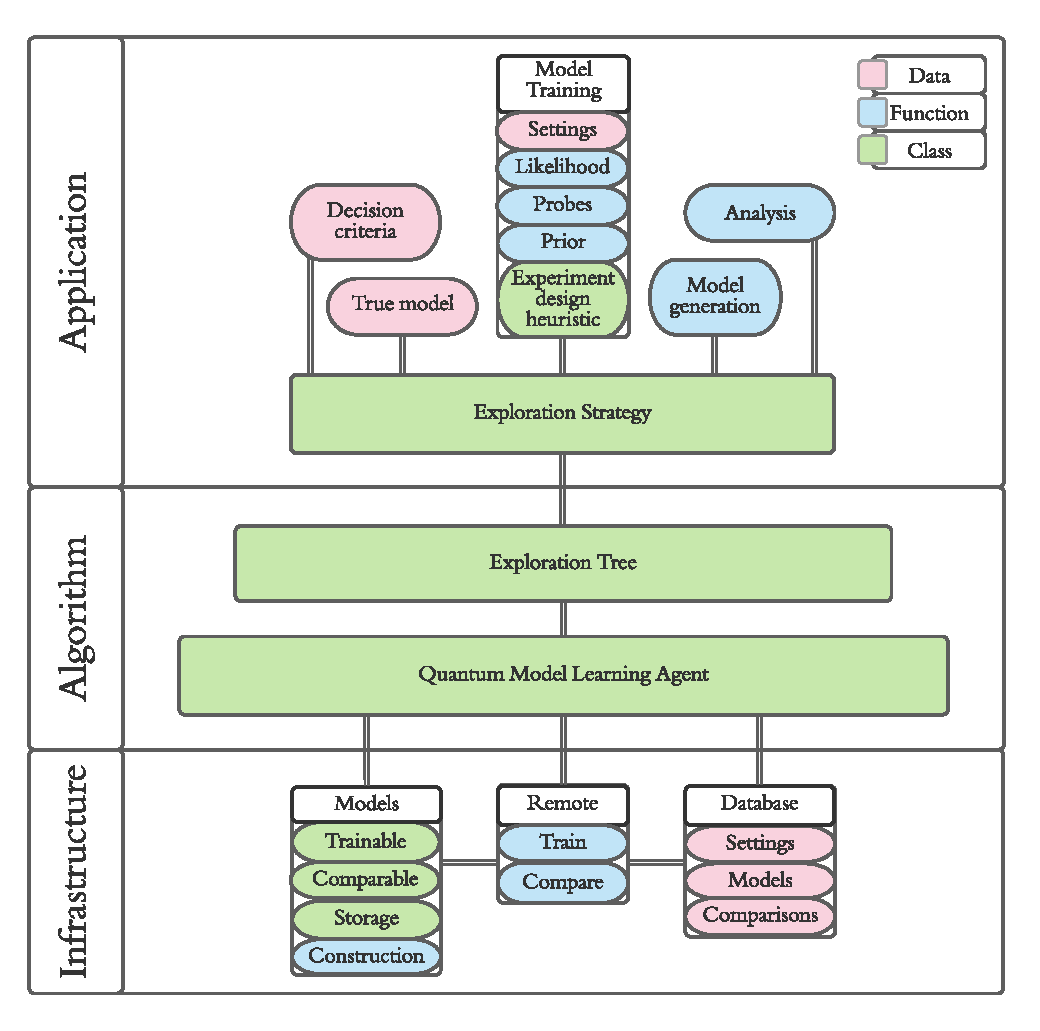
\includegraphics{algorithms/figures/software_overview.pdf}
    \caption[ \Glsentrylong{qmla} codebase overview]{
        Overview of important \emph{objects} in the \gls{qmla} framework.
        Colours encdoe the type of object: red objects are \emph{data}, blue are \emph{functions/methods} 
        and green are \emph{classes}. 
        Objects are grouped broady, with double lines showing communication channels between (groups of) objects. 
        \emph{Infrastructure}: functions for the implementation of model training/comparisons on 
        a remote server.
        \emph{Algorithm}: implementation of the iterative procedures and decision-making 
        laid out in \cref{chapter:qmla}. 
        \emph{Application}: inter-changeable data/functionality for the unique requirements 
        of a given target system. 
        Users wishing to customise \gls{qmla} must choose a valid object for each of those in \emph{applications}, 
            and need not alter any of the underlying framework.
    }
    \label{fig:software_overview}
\end{figure}

A driving motivation for the development of \gls{qmla} is generality:
    we endevaour to make \gls{qmla} applicable to any target quantum system.
We provide a framework, where users can tailor the inputs and methodology to their needs:
    we depict the main components of the framework in \cref{fig:software_overview}, 
    broadly grouping concepts as part of its \emph{infrastructure}, \emph{algorithm}
    or \emph{application}. 
In short, users need only specify the elements of the framework in the \emph{application} segment, 
    without concern for the underlying mechanics of \gls{qmla}; 
    in particular, users interface with the framework through the design of a bespoke \gls{es}, described next. 


\subsection{Application}\label{sec:application}
The application of \gls{qmla} refers to the choice of target system, $Q$, and how \gls{qmla} searches the 
    \gls{ms} in attempt to discover its model. 
As outlined in \cref{sec:exploration_strategies}, \glspl{es} play the role of 
    defining \gls{qmla}'s objectives, guiding the steps it takes, and designing the models to be tested. 
We facilitate the study of any system by providing a robust \ttt{ExplorationStrategy} base class,
    with all of the functionality expected of a generic \gls{es}, allowing users to inherit and build upon it. 
In particular, \glspl{es} allow users to specify the implementation of aspects listed in \cref{sec:exploration_strategies}, 
    as well as further details.
\par 


\subsubsection{Modular functionality}\label{sec:modular_functionality}
The most crucial methods\footnotemark \ of the \gls{es} class are modular, 
    described in \cref{sec:modular_functionality},
    meaning that they can be directly replaced, provided the alternative method fulfils the same role. 
Our base \gls{es} class uses sensbile defaults for this modular functionality, 
    but this flexible mechanism allows for adapting \gls{qmla} by choosing an approach for each 
    of the following subroutines. 
\footnotetext{
    The words \emph{method} and \emph{function} are mostly interchangeable, although methods are specifically associated with a class, 
    while functions are stand-alone.
}

\begin{easylist}[itemize]
    & Likelihood function. By default, \gls{qhl} calls a subroutine to compute \cref{eqn:likelihood}. 
        This can be replaced by any function which, given a Hamiltonian, evolution time and probe state, 
        returns the likelihood, according to the experiment you wish to simulate. 
        For example, in \cref{chapter:nv}, the data on which models are trained comes from experimental measurements, 
            so we replace the likelihood function with a calculation corresponding to the experimental procedure. 
        Importantly, QInfer requires the quantity $\Pr(0)$, see \cref{eqn:pr0}, so that is the output of these functions. 
    & Probe generation. The training phase requires a set of probes against which to optimise individual models. 
        Users may wish to specify the design of such probes, for example to match experimental constraints 
        which restrict the realisible probes in the performance of the experiment. 
        Alternatively, it may be feasible to design probes which increase the information gained per experiment, 
        enabling faster learning. 
    & \Glsentryfull{edh}. The choice of \gls{edh} greatly influences how the training will perform. 
        We provide a base class implementing \gls{pgh}, as well as child classes for each of 
        the \glspl{edh} listed in \cref{sec:alt_heuristics}. 
    & Prior. The method of drawing the prior distribution can be replaced, for example, with 
        a method for constructing a uniform distribution on each parameter.
        A key input to the procedure is the initial knowledge the user has about the system, 
        which is encoded in the prior, for instance varying orders of magnitude of the viable terms.
\end{easylist}

Additionally, applications require a series of settings for the model training phase, 
    such as the hyperparameters required by the resampling algorithm, \cite{liu2001combined}, 
    as well as detailing the true (target) model, $\ho$, in the case where $Q$ is a simulated quantum system.
We can also specify some \gls{es}-specific analyses to examine its internal performance, 
    although this is generally required during development/testing, and less useful thereafter. 

\subsection{Algorithm}\label{sec:sw_algorithm}
The algorithm layer of \cref{fig:software_overview} implements the core steps of \gls{qmla},
    as shown in \cref{fig:qmla_overview}, by running a set of \glsentryfullpl{et}, 
    each of which communicate with a unique \gls{es}. 
The core \gls{qmla} class manages the database of models and their comparisons,
    and decides how to react at certain stages, by consulting the decision criteria set by the \gls{es}. 
\par 

\subsubsection{Parallel implementiation}\label{sec:parallel}
\begin{figure}
    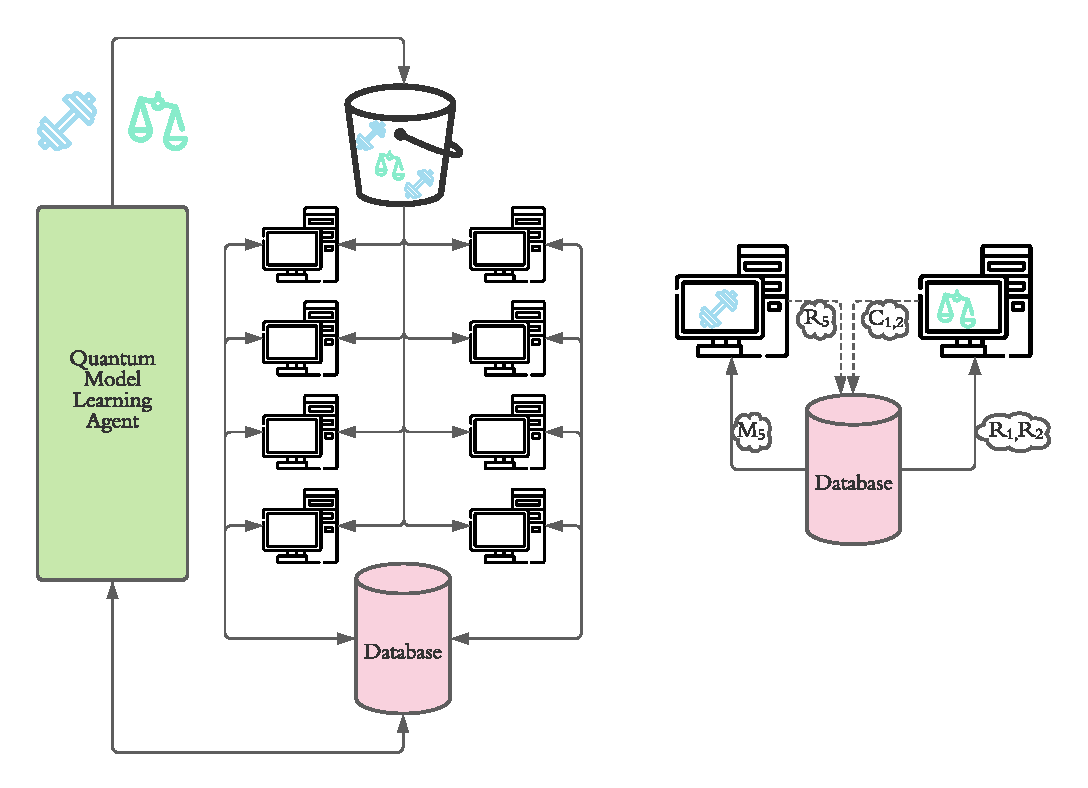
\includegraphics{algorithms/figures/parallel_architecture.pdf}
    \caption[Parallel architecture for \gls{qmla}]{
        Parallel architecture for \gls{qmla}.
        \textbf{Left}, \gls{qmla} generates tasks 
            -- either to train (blue dumbbells) or compare (oragne scales) models -- 
            and places them in a task queue. 
        Worker processes (depicted as computers) retrieve those tasks and compute them in parallel, 
            and interact with a database. 
        \textbf{Right}, Distributed tasks occuring in parallel. 
        The left-hand process assumes the task of training the model with ID 5:
            it first queries the database for a packet of core information, $M_5$, 
            which informs the model training procedure, for example the terms and parameters 
            of model 5. 
        After training, it sends a packet, $R_5$, summarising the result of model 5's training. 
        The right-hand process compares two models with IDs 1 and 2, by first retrieivng the results packets
            $R_1, R_2$, then storing the comparison $C_{1,2}$ on the database. 
    }
    \label{fig:parallel}
\end{figure}

The implementation of \gls{qmla} seeks to separate the organisation of the \gls{ms} from the 
    cumbersome calculations which enable the search. 
We can offload those calculations to a compute cluster (server) to run \emph{in parallel},
    allowing for significant speedup of the entire \gls{qmla} procedure, 
    limited by Amdahl's law. % TODO reference/explain Amdahls law (do we need it here? somewhere else?) 
\gls{qmla} distributes jobs to \emph{worker} processes in a server, 
    i.e. we assume that \gls{qmla} is run on a machine with $N_c$ available parallel \emph{processes}\footnotemark. 
Then, the expensive calculations, namely training and comparing models, are not performed 
    directly within the \gls{qmla} class, but instead are farmed out across the server.
The role of \gls{qmla} then is to collate the outcome of those calculations in conjunction with the set of \glspl{et}, 
    until each \gls{et} is deemed complete, and then to consolidate the set of 
    \gls{et} champions, ultimately setting the global champion, $\hp$. 
Thereafter it can perform some analysis, e.g. to generate a series of plots which demonstrate how the 
    model search progressed, as well as the evidence in favour of $\hp$, including for example 
    the reproduction of $Q$'s dynamics by $\hp$. 
See \cref{sec:qmla_analysis} for further details. 

\footnotetext{Note when running in \emph{serial} (e.g. running locally on a personal machine), it is valid to simply set $N_c=1$.}
\par 

While there are a number of strategies for parallelising code over a cluster, 
    we use the \emph{master-worker} strategy, where one process acts as the \emph{master}, 
    determining which calculations are required at any given moment, 
    then brokering self-contained tasks to \emph{workers}, 
    which blindly solve a small problem, without knowledge of the wider context or algorithm \cite{hockney2019parallel}.
The mapping here is trivial: the master of our algorithm is \gls{qmla}, 
    while workers can be used for the tasks of training and comparing models. 
The \gls{qmla} class is hence assigned a single process solely for its considerations, 
    e.g. for the ranking of models and determination of the next models to tests, 
    while the remaining $N_c - 1$ processes lay dormant until \gls{qmla} requests that they perform a job. 

\par 
We use a simple \emph{task queue} for the distribution of jobs: 
    \gls{qmla} adds tasks to the queue and any available worker can take the next job and compute it. 
There are two types of task for workers:
\begin{easylist}
    & to train a candidate model $\hi$:
        the worker first requests some essenital information about the model from the databse, 
        e.g. the name, terms and prior associated with the model, packaged in $M_i$;
        following completion, the worker compresses the result, $R_i$, and sends it to the database for storage. 
    & to compare two models, $\hi, \hj$: 
        the worker retrieves $R_i, R_j$ from the database, performs the calculation, 
        and returns the compressed outcome of the comparison, $C_{ij}$, to the database. 
\end{easylist}
The master \gls{qmla} class can also access said database, and copies the compressed results packets $R_i$ and $C_{ij}$,
    in order to account for the results in its decision-making. 
It is worth noting that tasks are completely independent, so some worker processes
    may compute comparisons while others train models simultaneously, 
    although obviously the comparison can not begin until both $R_i, R_j$ are available. 
This is dealt with easily by using a \emph{blocking} protocol, 
    where new batches of jobs are not released until the master receives all the results of jobs on which the new tasks depend.
\gls{qmla} simply waits until all models on a given layer have been trained before queueing comparisons 
    on that layer, to ensure a comparison can not start without the data needed to compute that comparison. 
\par

Models are assigned a unique ID upon creation; 
    models are uniquely described by their name, represented as a string in the \gls{qmla} class, 
    such that newly proposed models can be checked against the set of previously considered models 
    before being added to the database. 
\gls{qmla} can hence check whether a proposed model has already been trained, 
    in which case it does not resubmit the model, but instead relies on the previous result. 
Likewise \gls{qmla} can check for the presence of any comparison result $C_{ij}$ before setting it as a new task, 
    ensuring we do not duplicate expensive calculation. 
\par 
We use a redis database and task queue \cite{redis, redis_queue}. 
We depict the structure of this parallel architecture, and the master-worker strategy, in \cref{fig:parallel}.

\subsection{Infrastructure}\label{sec:infrastructure}
The infrastructure enabling the distribution of \gls{qmla}'s tasks across 
    a set of worker processes can be summarised as
\begin{easylist}
    & a set of classes representing the objects on which we must perform expensive calculations;
    & functions to launch those calculations independently of any other calculation;
    & a database which can be accessed by all workers as well as \gls{qmla}.
\end{easylist}
\par 

We need a series of distinct classes to represent models, for use in each stage of \gls{qmla}: 
    a \emph{trainable} class is used for the parameter optimisation, 
    while \emph{comparable} classes are used for computing \glspl{bf}, 
Crucially, this separation allows us to perform data-heavy calculations independently, 
    e.g. on a remote process within a compute cluster, 
    and discard the class instance used for the calculation and the large amount of data it generates, 
    while only the relatively small \emph{storage} classs is retained by \gls{qmla} for later use. 

\par 
The tasks which actually implement the calculations (\cref{sec:parallel}) are captured by standalone \emph{remote} functions. 
These functions receive instructions such as \ttt{train model 10}; 
    they then contact the database for the set of shared settings, 
    such as $\Ne, \Np$ and the set of probes, 
    before performing the task, and then sending the compressed result to the database for storage. 

\par 
To achieve this separation between calculation and analysis, we use a redis database \cite{redis},
    which holds the core implementation settings, e.g. $\Ne, \Np$ and the set of probes to train upon, 
    as well as the compressed summaries of the outcomes of tasks

\section{Usage}

Several aspects of \gls{qmla} are \emph{probabilistic}.
Firstly, the Bayesian updates within model training of \gls{qhl} relies on Likelihoods which 
    implicitly depend on the measurement datum of a quantum system; 
    in the case where the the measurement collapses $Q$ into the less-likely basis, 
    the likelihoods will reflect that accurate hypotheses were poor, 
    resulting in misguided posterior distributions. 
It is thus \emph{possible} that the parameter learning will converge on incorrect values. 
Moreover, the model design subroutine is not gauranteed to exploit the aspects of favoured models which are 
    actually informative, e.g. given a favoured model with four correct terms and two incorrect terms, 
    the model generator may opt to build on the incorrect terms, in the common situation where it does not know 
    which constituent terms are helpful and which aren't. 
\par 
Overall, then, it is pertinent to run \gls{qmla} many times and gather statistics about its performance, 
    rather than making overly-strong claims about $Q$ based on a single \emph{instance} of the algorithm. 
We say that a \gls{qmla} \emph{\gls{run}} consists of $N_r$ independent \emph{\glspl{instance}},
    which can be run in parallel, such that we are primarily concerned with the performance of the run 
    instead of any individual instance. 
For example, with $N_r=100$, we can interpret the \emph{\gls{win rate}} of every model in the model space
    as evidence for that model being $\ho$.
For the sake of evaluating \gls{qmla} itself, as in \cref{part:theoretical_study}, 
    we can use the \gls{win rate} of $\ho$ as indication of the \emph{\gls{success rate}}, 
    i.e. the fraction of instances within a run where \gls{qmla} identifies precisely $\hp = \ho$. 
Note, however, that neither the \gls{win rate} nor \gls{success rate} are singularly informative 
    of \gls{qmla}'s performance: in some cases, we can deem \gls{qmla} successful even if it does not 
    identify $\ho$ exactly, e.g. if it finds the majority of terms present in $\termset_0$ from a large space, 
    i.e. a high $\fs$, see \cref{sec:f_score}. 


\subsection{Outputs and analysis}
When a \gls{run} is launched, \gls{qmla} generates a \emph{\gls{results directory}} unique to that \gls{run}, 
    identified by the time and date of its launch,
    in which all the pertinent information for that \gls{run}, including raw data and figures, are stored. 
It includes an \ttt{analyse.sh} script to generate analysis after all instances have completed\footnotemark. 
\gls{qmla} provides a large amount of anaytics to assess the performance of the protocol. 
These range from \emph{big picture} perspectives such as the \gls{win rate} across the entire \gls{run}, 
    to zooming in on the internal metrics for training individual models.
Some of these analyses are generated by default, while others are optional depending on the 
    level of detail the user requires. 
A number of sub-directories are produced in the \gls{results directory}, 
    each containing data/figures from a different view of the \gls{run};
    these are listed in \cref{apdx:figure_repoduction}.
\footnotetext{
    Note this script is not run automatically since, on remote servers, instances finish independently without any central process
    noticing. Therefore this script must be run by the user when the run is complete.
}
\par 

The user has control on which plots are generated, in order that the appropriate level of degree is 
    presented, without producing an excessive number of images which can slow the protocol down. 
Results are categorised across the levels of the framework, for example:
\begin{easylist}
    & Run: results across a number of instances.
    && the number of instance wins for champion models.
    && average dynamics reproduced by champion models.
    & Instance: performance of a single insance.
    && models generated and the branches on which they reside
    & Model: Individual model performance within an instance.
    && parameter estimation through QHL.
    & Comparisons Pairwise comparison of models’ performance.
    && dynamics of both candidates (with respect to a single basis).
    & Exploration strategy: figures specific to the \gls{es}
    && model generation metrics
\end{easylist}
\par 

Most plots used in this thesis are generated directly by the \gls{qmla} framework\footnotemark; 
    the \gls{es} class and implementation parameters of each figure is listed in \cref{table:figure_reproduction}.
\footnotetext{Or are minor modifications of auto-generated plots.}


\part{Theoretical Study}\label{part:theoretical_study}
    \chapter{Prescribed model sets}\label{chapter:lattices}
        A sensible first case study for the \gls{qmla} framework is to prescribe a set of models, 
    where we know that the true model is among them, or at least that we would be satisfied with 
    approximating $\ho$ as the best model in the set. 
This application can be useful, for example, for expedited device calibration; 
    suppose we wish to characterise a new, \epmh{untrustued} quantum simulator/device, $S_u$, 
    and we have access to a \emph{trusted}\footnotemark \  simulator, $S_t$. 
In order to perform this calibration, 
    we treat $S_u$ as the system, $Q$, i.e. we call upon it to retrieve the datum $d$ in \cref{eqn:likelihood}, 
    where the calculation of the likelihoods for each particle are computed through $S_t$. 
If $S_u$ is reliable, the data from its calculations will be consistent with some $\ho$ of our choosing, 
    while miscalibrations will mainfest as imperfectly implemented gates/steps in the calculation of the system's likelihood, 
    and so would result in data inconsistent with $\ho$. 
Therefore, if we can prescribe the most likely miscalibrations, it may be feasible to compose a set 
    of models, $\mathbb{H}$, which represent those cases, and search for $\hp$ only within $\mathbb{H}$,
    to find identify the miscalibrations. 
For example, by encoding connections between every pair of device qubits in $\ho$, 
    we can compose models with restricted connectivity, for instance where some pairs of qubits are disconnected, 
    and hence discover whether the device allows arbitrary two-qubit gates, 
    and which pairs are disallowed. 

\footnotetext{Note: here a classical computer can fulfil the role of the trusted simulator.}


\section{Lattices}\label{sec:lattices}
We first consider $Q$ as some lattice, where \gls{qmla} attempts to identify the structure of the lattice. 
The set of viable models then comprises alternative lattices.
Due to simluation constraints, because we train models through exact unitary evolution, 
    we are restricted to $\sim~8$-qubit Hamiltonians, so we only consider lattices which can 
    be simulated in this limit. 
The \gls{es} in this chapter is then simply to propose a set of models with no further model generation, 
    with comparisons between all pairs of models through \glspl{bf}.
\par

Connectivity between lattice sites is achieved within the specific Hamiltonian formalisms
    introduced in the following sections, 
    although in general we write $\mathcal{C} = \{\bkl \}$ as the set of connected pairs $\bkl$, 
    such that the Hamiltonian for a given lattice can be thought of as 
    some function of its configuration, $\hat{H}\bk{\al, \mathcal{C}}$.
Then, we can specify candidate models only by their $\mathcal{C}$, 
    e.g. a 3-site chain can be summarised by $\mathcal{C}= \{ \langle 1,2 \rangle, \langle 2,3 \rangle\}$, 
    whereas a fully connected 3-site lattice (i.e. a triangle) is given by 
    $\mathcal{C}= \{ \langle 1, 2 \rangle, \langle 1, 3 \rangle, \langle 2, 3 \rangle\}$. 
We can then summarise the set of candidate models through the descriptions of lattice configurations, 
    corresponding to those depicted in \cref{fig:lattices}:
\begin{easylist}
    \ListProperties(Numbers=l)
    & 2-site chain
    & 3-site chain
    & 3-site fully connected (triangle)
    & 4-site fully conneted (square)
    & 4-site linearly connected (loop)

    & 4-site chain
    & 5-site chain
    & 6-site chain
    & 5-site fully connected (pentagon)
    & 6-site partially connected (grid)
\end{easylist}


\begin{figure}
    \begin{center}
        \begin{subfigure}{2.25cm}
            \begin{center}
                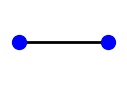
\includegraphics{theoretical_study/figures/lattices/_2_site_chain.jpg}                        
            \end{center}
            \caption{}
        \end{subfigure}
        \qquad
        \begin{subfigure}{2.25cm} 
            \begin{center}
                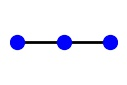
\includegraphics{theoretical_study/figures/lattices/_3_site_chain.jpg}
            \end{center}
            \caption{}
        \end{subfigure}
        \qquad
        \begin{subfigure}{2.25cm} 
            \begin{center}
                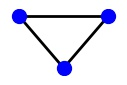
\includegraphics{theoretical_study/figures/lattices/_3_site_lattice_fully_connected.jpg}        
            \end{center}
            \caption{}
        \end{subfigure}
        \qquad
        \begin{subfigure}{2.25cm} 
            \begin{center}
                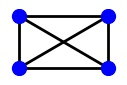
\includegraphics{theoretical_study/figures/lattices/_4_site_lattice_fully_connected.jpg}        
            \end{center}
            \caption{}
        \end{subfigure}
        \qquad
        \begin{subfigure}{2.25cm} 
            \begin{center}
                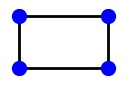
\includegraphics{theoretical_study/figures/lattices/_4_site_square.jpg}        
            \end{center}
            \caption{}
        \end{subfigure}
        \\
        \begin{subfigure}{2.25cm} 
            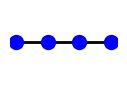
\includegraphics{theoretical_study/figures/lattices/_4_site_chain.jpg}        
            \caption{}
        \end{subfigure}
        \qquad
        \begin{subfigure}{2.25cm} 
            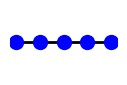
\includegraphics{theoretical_study/figures/lattices/_5_site_chain.jpg}        
            \caption{}
        \end{subfigure}
        \qquad
        \begin{subfigure}{2.25cm} 
            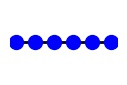
\includegraphics{theoretical_study/figures/lattices/_6_site_chain.jpg}        
            \caption{}
        \end{subfigure}
        \qquad
        \begin{subfigure}{2.25cm} 
            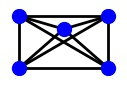
\includegraphics{theoretical_study/figures/lattices/_5_site_lattice_fully_connected.jpg}        
            \caption{}
        \end{subfigure}
        \qquad
        \begin{subfigure}{2cm} 
            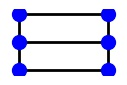
\includegraphics{theoretical_study/figures/lattices/_6_site_grid.jpg}        
            \caption{}
        \end{subfigure}
    \end{center}
    \caption[Lattices for prescribed QMLA]{
        Lattices used for prescribed models test for \gls{qmla}.
        Lattices are characterised by the connectivity of their sites; 
            dotted lines show connection between pairs of sites.                 
    }
    \label{fig:lattices}
\end{figure}

We will use this set of lattice configurations throughout the remainder of this chapter. 

\section{Ising model}\label{sec:ising}
The Ising model is one of the most studied concepts in all of physics, 
    representing electrons on a lattice of $N$ sites, 
    where each electron can have \emph{spin} up or down 
    \cite{ising1925beitrag, onsager1944crystal, brush1967history}.
Interactions between spins $\bkl$ have strength $J_{kl}$, 
    and the transverse magnetic field acts on spin $k$ with strength $h_k$. 
It is usually stated as 
\begin{equation}
    \label{eqn:ising_standard_form}
    \hat{H}_I(\cc) = \sum_{\bkl \in \mathcal{C}} J_{kl}  \ \hat{\sigma}_k^z \ \hat{\sigma}_{l}^z + \sum_{k=1}^{N} h_k \hat{\sigma}_{k}^x.
\end{equation}

The interaction term indicates the class of magnetism of the pair's interaction, i.e. 
\begin{equation}
    \label{eqn:ising_magnetism_cases}
    \begin{cases}
        J_{kl} < 0, \ \ \textrm{ferromagnetic}; \\
        J_{kl} > 0, \ \ \textrm{antiferromagnetic}; \\
        J_{kl} = 0, \ \ \textrm{noninteracting}.
    \end{cases}
\end{equation}
If all interaction pairs are described by the same case in \cref{eqn:ising_magnetism_cases}, 
    the entire system can be said belong to that class of magnetism. 

\par 
\subsection{Note on optimising the Ising model}\label{sec:ising_optimisation}
Many treatments of the Ising model seek to find the ground state
    of the system by optimising the configuration of spins in the system. 
This involves neglecting the transverse magnetic field, and treating Ising model classically, 
    such that the ground state is found by minimising the energy function
\begin{equation}
    \label{eqn:ising_energy_function}
    E_I = \braket{\psi | H_I | \psi} = 
    \sum_{\bkl \in \mathcal{C}} J_{kl}  \ \braket{ \psi |  \hat{\sigma}_k^z \ \hat{\sigma}_{l}^z | \psi }, 
\end{equation}
    where $\ket{\psi} = \ket{\psi_1} \otimes \ket{\psi_2} \dots \otimes \ket{\psi_N}$. 

This optimisation relies on the relationship between the Ising model with its eigenvalues and eigenstates:
    \cref{eqn:ising_energy_function} consists only of $\sz$ terms, and we have that 
\begin{equation}
    \sz \ket{+} = +1 \ket{+} \ \ \ ; \ \ \ 
    \sz \ket{-} = -1 \ket{-}. 
\end{equation}

Then, for a single pair of spins $\bkl$, we have
\begin{equation}
    \label{eqn:ising_spin_cases}
    \begin{split}
        \bra{+_k \ +_l } \sz_k \ \sz_l  \ket{+_k \ +_l } =  \bra{+_k \ +_l } (+1)(+1) \ket{+_k \ +_l } = +1, \\
        \bra{+_k \ -_l } \sz_k \ \sz_l \ket{+_k \ -_l } = \bra{+_k \ -_l } (+1)(-1) \ket{+_k \ -_l } = -1 , \\
        \bra{-_k \ +_l } \sz_k \ \sz_l \ket{-_k \ +_l } = \bra{-_k \ +_l } (-1)(+1) \ket{-_k \ +_l } = -1, \\
        \bra{-_k \ -_l } \sz_k \ \sz_l \ket{-_k \ -_l } = \bra{-_k \ +_l } (-1)(1) \ket{-_k \ -_l } = +1. \\
    \end{split}
\end{equation}
So, by restricting the individual spins to $\ket{\psi_k} \in \{\ket{+}, \ket{-}\}$, 
    we can equivalently consider every spin $s_k$ in the system
    as a binary variable $s_k \in \{\pm 1\}$,
    i.e. $s_k s_l = \pm 1$ in \cref{eqn:ising_spin_cases},
    such that the energy function
\begin{equation}
    \label{eqn:ising_energy}
    E_I(\mathcal{S}) = \braket{ \psi | \hat{H}_I | \psi } = \sum\limits_{\bkl \in \cc} J_{kl} \ \ s_k s_l
\end{equation}
    can be minimised by optimising the configuration $\mathcal{S}$, when the interaction terms $\{J_{\bkl}\}$ are known.
The optimal configuration $\mathcal{S}_0$ can then be mapped to a 
    state vector $\ket{\psi_0}$, i.e. the ground state of the system. 
\par 

While this task can be greatly simplified by the reduction in \cref{eqn:ising_spin_cases}, 
    meaning we do not have to compute any unitary evolution to evaluate \cref{eqn:ising_energy},
    it is still an expensive optimisation, because effectively it is a search over $\{ \ket{\psi }\}$, 
    so the search space has $2^N$ candidates \cite{onsager1944crystal, barahona1982computational}. 
This allows for a straightforward mapping between ground state search 
    and solving combinatorial optimsiation algorithms, namely \ttt{MAX-CUT}, 
    known to be NP-complete \cite{garey1979computers}, 
    allowing for proposed advantage in mapping computationally challenging problems to quantum hardware \cite{lucas2014ising}. 
This mapping underlies ongoing research into quantum annealing as a computational platform capable of providing 
    advantage for a specific family of problems \cite{santoro2006optimization, bapst2013quantum, johnson2011quantum}. 
\par

Crucially, our goal is \emph{not} to find the ground state of $Q$, 
    but instead to find the generator of its dynamics.
Therefore, we treat the Ising \emph{quantum mechanically}:
    instead of treating \cref{eqn:ising_standard_form} as the underlying mechanism for a cost function 
    to be optimised, i.e. \cref{eqn:ising_energy}, 
    we use quantum operators and do not necessarily restrict the \gls{probe} state $\ket{\psi}$, 
    allowing us to use \cref{eqn:ising_standard_form} within the likelihood function \cref{eqn:likelihood}.

\subsection{Ising model cases}

We consider two cases: 
    firstly, where it is assumed that the strength of interactions $J_{k,l}$ are uniform (given by $J$);
    and secondly, where each interaction is assigned a unique parameter ($J_{kl}$).
In the first case, we can represent the Ising model for a given lattice configuration $\cc$ as 
\begin{equation}
    \label{eqn:ising_model_full}
    \hat{H}(\mathcal{C}) = 
        J \sum\limits_{\bkl \in \mathcal{C}} \s^{z}_{k} \s_{l}^{z} 
        + h \sum\limits_{k=1}^{N} \s^{x}_{k}, 
\end{equation}    
    allowing for the compact representation, following \cref{sec:models},
\begin{subequations}
    \label{eqn:ising_terms}
    \begin{equation}
        \vec{\alpha}_I = \irow{ J & h }
    \end{equation}
    \begin{equation}
        \terms_I = \icol{ 
            \sum\limits_{\bkl \in \mathcal{C}} \s^{z}_{k} \s_{l}^{z} \\
            \sum\limits_{k=1}^{N} \s^{x}_{k}
        }. 
    \end{equation}
\end{subequations}

In the more general second case, termed the \emph{fully parameterised} Ising model, we instead have the term set
\begin{equation}
    \label{eqn:ising_fully_parameterised}
    \termset_I = \left\{ 
        \s^{z}_{k} \s_{l}^{z}, \ \
        \sum\limits_{k=1}^{N} \s^{x}_{k}
    \right\}\limits_{\bkl \in \cc}. 
\end{equation}
    with unique parameters $J_{kl}$ associated with each interaction term $\s_k^z \s_l^z$. 
We summarise these cases in \cref{table:ising_models}.

\begin{table}[H]
    \begin{center}
        \begin{tabular}{crr}
             & $J_{\bkl}$  & $h_{k}$ \\
            \hline
            Standard & $J$ & $h$ \\
            Fully parameterised & $J_{\bkl}$ & $h_{k}$
        \end{tabular}
    \end{center}
    \caption[Types of Ising model]{Types of Ising model. Varying whether parameters $J^{z}_{\bkl}, h_k$ are shared 
        across sites gives distinct models. 
    }
    \label{table:ising_models}
\end{table}

\par 

\begin{figure}
    \begin{center}
        \QMLAfig{Nov_18/13_56/standard_ising_qhl.pdf}
    \end{center}

    \caption[\gls{qhl} for Ising model]{
        \gls{qhl} for Ising model where terms are grouped by their functionality, 
        as in \cref{eqn:ising_standard_form}. 
        (a,b) show the parameter estimates progression against 
        epochs (experiments), with the corresponding term written on top of the plot; 
        (c) shows the \gls{volume} of the parameter distribution at each epoch, as well as the 
        evolution time chosen by the \gls{edh}. 
        \figtableref
    }
    \label{fig:ising_two_param_learning}
\end{figure}

\begin{figure}
    \begin{center}
        \QMLAfig{Nov_18/13_56/fully_param_ising_qhl.pdf}        
    \end{center}
    \caption[\gls{qhl} for Ising model]{
        \gls{qhl} for fully parameterised Ising model, 
            where every interaction between pairs of sites are assigned unique parameters, 
            here neglecting the transverse field, 
            as in \cref{eqn:ising_fully_parameterised}. 
        (a)-(f) show the parameter estimates progression against 
        epochs (experiments), with the corresponding term written on top of the plot; 
        (g) shows the \gls{volume} of the parameter distribution at each epoch, as well as the 
        evolution time chosen by the \gls{edh}. 
        \figtableref
    }
    \label{fig:ising_fully_parameterised}
\end{figure}

\begin{figure}
    \begin{center}
        \QMLAfig{Nov_18/13_56/dynamics.pdf}
    \end{center}
    \caption[Ising model types' dynamics.]{
        Dynamics reproduced by Ising models under standard and fully parameterised formalisms, 
        compared with dynamics for the true system.
        \figtableref
    }
    \label{fig:ising_model_types_dynamics}
\end{figure}


We first construct models under each of these forms to verify \gls{qhl} is capable of learning in this regime. 
The former case is the standard form of the Ising model; its training is shown in \cref{fig:ising_two_param_learning}, 
    while the fully paramterised model is shown in \cref{fig:ising_fully_parameterised}. 
Ultimately, these two cases give the same Hamiltonian when $J_{\bkl} = J; \ h_k = h \ \forall k,l$.
So, the fully parameterised model will learn the same parameters as the standard Ising model,
    and we can take the \gls{bf} between them to determine which parameterisation is favourable.
Encouragingly, both models learaned the parameters to high precision, and neither model converged; 
    the \gls{volume} continues to reduce exponentially in both cases, 
    suggesting it may be impractical to seek saturation in the model training phase for every model, 
    since this may require a very large number of experiments and particles. 
\par 

The dynamics produced by both models are shown in \cref{fig:ising_model_types_dynamics}:
    the dynamics are almost indistinguishable by eye, but the standard Ising model, 
    which in this case is $\ho$, outperforms the fully parameterised model, 
    by a \gls{bf} of $10^{19}$.
This serves as a good \emph{sanity check}, confirming our expectation that 
    the \gls{bf} will favour the simpler model (i.e. fewer parameters) even when both models 
    are trained to a high precision to very similar parmaeters, and are difficult to distinguish through human intuition. 


\section{Heisenberg model}\label{sec:heisenberg}
Generalising the Ising model, the Heisenberg Hamiltonian is another model for magnetic systems consisting of a set of 
    spins on a lattice \cite{greiner2012thermodynamics}. 
It builds on the Ising model by additionally considering the spins' rotations about the $x-$ and $y-$ axes, generally stated as 
\begin{equation}
    \label{eqn:heisenberg_model_general}
    \hat{H}_H(\cc) = 
    \sum\limits_{\bkl \in \cc} J^x_{kl} \  \s^x_k \s^x_l
    + \sum\limits_{\bkl \in \cc} J^y_{kl} \ \s^y_k \s^y_l
    + \sum\limits_{\bkl \in \cc} J^z_{kl} \ \s^z_k \s^z_l
    + \sum\limits_{k=1}^{N} h_k \s^z_k.
\end{equation}

We can consider a number of formulations of the Heisenberg model, by considering whether the interaction
    parameters are completely unique for each pair of spins in each axis, 
    or  are shared by pairs of spins;
    we list the instances within the family of Heisenberg models in \cref{table:heisenberg_models}. 
\begin{table}[H]
    \begin{center}
        \begin{tabular}{crrrr}
             & $J^x_{kl}$ & $J^y_{kl}$ & $J^z_{kl}$ & $h_k$ \\
            \hline
            XXX & $J^x$ & $J^x$ & $J^x$ & $h$ \\
            XXZ & $J^x$ & $J^x$ & $J^z$ & $h$ \\
            XYZ (standard) & $J^x$ & $J^y$ & $J^z$ & $h$ \\
            Fully parameterised & $J^x_{kl}$ & $J^y_{kl}$ & $J^z_{kl}$ & $h_k$ \\
            
        \end{tabular}
    \end{center}
    \caption[Types of Heisenberg model]{
        Heisenberg model types: varying whether the interaction parameters $J^{w}_{kl}$ are shared among pairs of spins
        give distinct descriptions which are all in the family of Heisenberg models. 
    }
    \label{table:heisenberg_models}
\end{table}

Again, there are a number of possibile models to test, 
    although we can reasonably expect these to follow the same arguments as for the Ising model cases: 
    increasing generality at the expense of larger parameter dimension requires more resources to learn to a reasonable level. 
In this chapter we will refer to the Heisenberg-XYZ model,
    and will consider the fully parameterised Heisenberg model in \cref{chapter:ga};
    the parameters and terms of interest are then captured by \cref{eqn:heisenberg_terms}.


\begin{subequations}
    \begin{equation}
        \al_H = \irow{ J^x & J^y & J^z & h}    
    \end{equation}

    \begin{equation}
        \terms_H = \icol{
            \sum\limits_{\bkl \in \cc} \ \s^x_k \s^x_l \\
            \sum\limits_{\bkl \in \cc} \ \s^y_k \s^y_l \\
            \sum\limits_{\bkl \in \cc} \ \s^z_k \s^z_l \\
            \sum\limits_{k=1}^{N} \ \s^z_k  \\
        }
    \end{equation}
    \label{eqn:heisenberg_terms}
\end{subequations}


\section{Hubbard model}\label{sec:hubbard}
Another representation of solid state matter systems is given by the Hubbard model 
    \cite{hubbard1963electron, scalettar2016introduction, hubbard2013}.
The Hubbard model deals with systems of correlated fermions, 
    allowing spins to \emph{hop} between sites. 
Note the Hubbard model is synonymous with the \gls{fh} model, 
    which can be used to distinguish this model of fermions from a similar model of bosons, named the Bose-Hubbard model, 
    which is not studied in this thesis. 
We use the subscript FH to distinguish the (Fermi-)Hubbard model from the Heisenberg model $\hat{H}_{H}$, \cref{eqn:heisenberg_model_general}.
The Hubbard model is generally stated in second quantisation as

\begin{equation}
    \label{eqn:hubbard}
    \hat{H}_{FH}(\cc) = 
    \sum_{s \in \{\uparrow, \downarrow\}} \sum_{ \bkl \in \mathcal{C}} t^{s}_{\bkl} \left( \hat{c}^{\dagger}_{ks} c_{ls} + \hat{c}^{\dagger}_{ls} c_{ks} \right) 
    + \sum_{k}^{N} U_k \hat{n}\limits_{k\uparrow}\hat{n}_{k\downarrow} 
    + \sum_{k}^{N} \mu_k \left( \hat{n}\limits_{k\uparrow} + \hat{n}_{k\downarrow} \right)     
\end{equation}
    where 
\begin{easylist}[itemize]
    & $\hat{c}_{ks}$ and $\hat{c}^{\dagger}_{ks}$ are respecitvely the fermionic annihilation and creation operators for spin $s \in \{ \uparrow, \downarrow \}$ on site $k$;
    & $\hat{n}_{ks} = \hat{c}^{\dagger}_{ks} \hat{c}_{ks}$ is a counting operator to count the number of spins $s$ on site $k$;
    & $t^s_{\bkl}$ is the kinetic (hopping) term for spin $s$ between sites $k$ and $l$; 
    & $U_k$ is the onsite (repulsion) energy for site $k$;
    & $\mu_k$ is the chemical energy for $k$;
    & $N$ is the number of sites in the system.
\end{easylist}
\par

Again, we can achieve differing physics by controlling whether the parameters are shared, 
    with similar consequences to the Ising and Heisenberg models, where additional parameterisation
    comes at the expense of slower/worse performance in training. 
We list a subset of possible configurations in \cref{table:hubbard_model_types};
    we will use the standard form in this chapter, i.e. 

\begin{subequations}
    \begin{equation}
        \al_{FH} = \irow{ t^{\uparrow} & t^{\downarrow} & U & \mu}
    \end{equation}
    
    \begin{equation}
        \terms_{FH} = \icol{ 
            \sum\limits_{ \bkl \in \cc }
                ( 
                    \hat{c}^{\dagger}_{k,\uparrow} \hat{c}_{l,\uparrow} + \hat{c}^{\dagger}_{l,\uparrow} \hat{c}_{k,\uparrow} 
                ) \\
            \sum\limits_{ \bkl \in \cc }
                ( 
                    \hat{c}^{\dagger}_{k,\downarrow} \hat{c}_{l,\downarrow} + \hat{c}^{\dagger}_{l,\downarrow} \hat{c}_{k,\downarrow} 
                ) \\
            \sum\limits_{k=1}^{N} \hat{n}_{k\uparrow} \hat{n}_{k\downarrow} \\
            \sum\limits_{k=1}^{N} \bk{\hat{n}_{k\uparrow}  + \hat{n}_{k\downarrow} }
        }
    \end{equation}
    
    \label{eqn:hubbard_terms}
\end{subequations}

\begin{table}[H]
    \begin{center}
        \begin{tabular}{crrrr}
             & $t^{\uparrow}_{\bkl}$& $t^{\uparrow}_{\bkl}$ & $U_k$ & $\mu_k$ \\
            \hline 
            Standard & $t^{\uparrow}$ & $t^{\downarrow}$ & $U$ & $\mu$ \\
            Fully parameterised & $t^{\uparrow}_{\bkl}$  & $t^{\downarrow}_{\bkl}$&  $U_k$ & $\mu_k$ \\
        \end{tabular}
    \end{center}
    \caption[Types of Hubbard model]{
        Types of Hubbard model. Varying whether parameters $t^{s}_{\bkl}, U_k, \mu_k$ are shared 
        across sites gives distinct models.
    }
    \label{table:hubbard_model_types}
\end{table}

\subsection{Jordan Wigner transformation}\label{sec:jordan_wigner}
In order that the Hubbard model is simulateable with qubits\footnotemark, 
    it must first undergo a mapping from the fermionic 
    representation to a spin system representation; 
    such a mapping is given by the \gls{jwt} \cite{jordan1993paulische, steudtner2018fermion}.
We implement the \gls{jwt} within \gls{qmla} through \ttt{OpenFermion}'s \ttt{fermilib} package \cite{mcclean2020openfermion}.
\footnotetext{Or simulations of qubits, as in this thesis.}
\par 

In second quantisation, 
    the fermions on the lattice can occupy one (or a superposition of) \emph{modes}, 
    for example, spin $\uparrow$ on the site indexed $3$ is a mode. 
The system can then be given by a state in the \emph{number basis}, 
\begin{equation}
    \ket{\psi_f} = \ket{ n_{m_1}, n_{m_2}, \dots , n_{m_n} },
\end{equation}
where $n_{m_i}$ is the number of fermions on mode $m_i$ and there are $n$ modes in total.

$\hat{c}^{\dagger}_{m_i}$ \ ($\hat{c}_{m_i}$) is the creation (annihilation) operator
    on the mode $m_i$: it acts on the system by adding (removing) a fermion from (to) $m_i$:
\begin{subequations}
    \begin{equation}
        \hat{c}^{\dagger}_{m_i} \ket{\psi_f} = \ket{ n_{m_1}, \dots , n_{m_i}  + 1,  \dots , n_{m_n} }, 
    \end{equation}
    \begin{equation}
        \hat{c}_{m_i} \ket{\psi_f} = \ket{ n_{m_1}, \dots , n_{m_i} - 1,  \dots , n_{m_n} }.
    \end{equation}            
\end{subequations}

In the Hubbard model, we assign a mode for each combination of spin $s \in \{\uparrow, \downarrow\}$
    with each site $k$, i.e. the system is in the state
\begin{equation}
    \label{eqn:hubbard_number_state}
    \ket{\psi_{FH}} = \ket{ n_{1\uparrow}, n_{1\downarrow}, \dots , n_{N\uparrow}, n_{N\downarrow} }.
\end{equation}
\par 

In particular, since fermions obey the Pauli exclusion principle, 
    i.e. every spin/site can be occupied by at most one electron, and we can view them as two-level systems, 
    so we have $n_{sk} \in \{0, 1\} \forall s, k$,     
We therefore use a similar system to the number basis: 
    a qubit registered as $\ket{0}$ corresponds to an empty mode, while $\ket{1}$ holds a fermion. 
Empty lattices are thus given by $\ket{0}^{\otimes 2N}$. 
Then, in analogue with the annihilation and creation operators, we introduce oeprators $\s^{+}, \s^{-}$ such that 
\begin{subequations}
    \begin{equation}
        \s^{+} = \begin{pmatrix}
            0 & 0 \\ 1 & 0 
        \end{pmatrix}
        \Longrightarrow \s^{+} \ket{0} = \ket{1}
    \end{equation}

    \begin{equation}
        \s^{-} = \begin{pmatrix}
            0 & 1 \\ 0 & 0 
        \end{pmatrix}
        \Longrightarrow \s^{-} \ket{1} = \ket{0}
    \end{equation}
\end{subequations}
   

Then, to map the number basis of \cref{eqn:hubbard_number_state} to a state which can be prepared on qubits, 
    the \gls{jwt} assigns a single qubit to each mode, 
    where qubits are ordered simply by the site index and spin type, 
    as shown in \cref{table:jordan_wigner_indices}. 
The \gls{jwt} can be summarised by mapping -- for the mode $m$ -- the creation (annihilation) operator
    $\hat{c}^{\dagger}_{m}$ \ ($\hat{c}_{m}$), to an operator which adds a spin to the corresponding state 
    through the operator $\s_{m}^{+}$ \ ($\s_{m}^{-}$). 

\begin{subequations}
    \label{eqn:jordan_wigner}
    \begin{equation}
        \hat{c}_{m} \rightarrow (\s^z)^{\otimes k-1} \otimes \s^{-} \otimes (\s^z)^{\otimes 2N-1}
    \end{equation}
    \begin{equation}
        \hat{c}_{m}^{\dagger} \rightarrow (\s^z)^{\otimes k-1} \otimes \s^{+} \otimes (\s^z)^{\otimes 2N-1}
    \end{equation}
\end{subequations}

Note the \gls{jwt} acts on all modes/qubits other than the target with $\s^z$, since 

For example, an empty 2-site lattice $\ket{\psi_0}$ is acted on by a creation operator on mode $3$, corresponding to spin $\uparrow$ on site $2$:
\begin{equation}
    \hat{c}^{\dagger}_{2\uparrow} \ket{0000}  = \hat{c}^{\dagger}_{3} \ket{0000} = \s^z_1 \s^z_2 \s^{+}_3 \s^z_4 \ket{0000} = \ket{0010}
\end{equation}

\begin{table}
    \begin{center}
        \begin{tabular}{cccc}
            Mode & Site & Spin & Qubit \\
            \hline
            $1$ & $1$ & $\uparrow$ & $1$ \\
            $2$ & $1$ & $\downarrow$ & $2$ \\
            $3$ & $2$ & $\uparrow$ & $3$ \\
            $4$ & $2$ & $\downarrow$ & $4$ \\
             & \vdots &  & \\
            $2N -1$ & $N$ & $\downarrow$ & $2N-1$ \\
            $2N$ & $N$ & $\uparrow$ & $2N$ \\
        \end{tabular}
    \end{center}
    \caption[Jordan Wigner mode/qubit indices]{Jordan Wigner mode/qubit indices.}
    \label{table:jordan_wigner_indices}
\end{table}



\subsection{Half filled basis}
In principle there can be $2N$ spins on a lattice of $N$ sites, 
    although in general we will restrict to the case where there are $N$ spins in the lattice, 
    known as \emph{half-filling}, such that \cref{eqn:hubbard_number_state} is effectively projected into the subspace 
    spanned by half-filled basis states. 
For example, with $N=2$
\begin{equation}
    \label{eqn:hubbard_half_filled_basis_states}
    \{
        \ket{ 1100 }, \ket{ 1010 }, \ket{ 1001 }, 
        \ket{ 0101 }, \ket{ 0110 }, \ket{ 0011 }
    \}
\end{equation}

Therefore, in the design of probes for training Hubbard models, 
    we can generate probes in the subspace spanned by half-filled states. 

\section{Model learning for lattices}
Finally, then, we can use the lattice systems introduced in \cref{sec:lattices,sec:ising,sec:heisenberg,sec:hubbard}
    as first case studies for \gls{qmla}. 
Each $\cc \in \mathbb{C}$ can specify a unique model under the standard model formalism
    for each of Ising (\cref{eqn:ising_terms}), Heisenberg (\cref{eqn:heisenberg_terms}) 
    and Hubbard (\cref{eqn:hubbard_terms}) models.     
We can then devise a simple \gls{es} which only tests the models corresponding to $\mathbb{C}$, 
    with no further model generation, i.e. \cref{alg:lattice_exploration_strategy}, 
    and compares every pair of models through \gls{bf}, 
    deeming the champion as that which wins the largest number of comparisons, 
    as in \cref{alg:lattice_exploration_strategy_consolidation}.

\begin{algorithm}
    \caption{Lattice exploration strategy: model generation}
    \label{alg:lattice_exploration_strategy}
    \DontPrintSemicolon
    \KwIn{ $\mathbb{C}$ \tcp*[1]{Set of lattice configurations}}

    \KwOut{$\{ \hi \}$ \tcp*[1]{Set of models to tests}}\;

    $\mathbb{H}$ = \{ \}\;
    \For{$\cc \in \mathbb{C}$}{
        $\hi \gets$ \ttt{map\_lattice\_to\_model}($\cc$)\;
        $\mathbb{H} \gets \mathbb{H} \cup \{ \hi\}$
    }
    return $\mathbb{H}$
\end{algorithm}

\begin{algorithm}
    \caption{Lattice exploration strategy: consolidation}
    \label{alg:lattice_exploration_strategy_consolidation}
    \DontPrintSemicolon
    \KwIn{ $\mathbb{H}$ \tcp*[1]{Set of trained models}}

    \KwOut{$\hp$ \tcp*[1]{Favoured model}}\;

    \For{ $\hi \in \mathbb{H}$}{
        $s_i \gets 0 $ \tcp*[1]{Score for every model}
    }

    \For{$\hi \in \mathbb{H}$}{
        \For{$\hj \in \mathbb{H}\setminus \{\hi\}$}{
            $\bij \gets BF(\hi, \hj)$ \tcp*[1]{Compute Bayes factor via \cref{alg:bayes_factor}}

            \If{$\bij > 1$}{
                $s_i \gets s_i + 1$ \tcp*[1]{$\hi$'s score increases if it is the stronger model}
            }
        }
    }
    $\hp \gets \argmax\limits_{s_i} \bk{\hi}$

    return $\hp$
\end{algorithm}


\begin{figure}
    \QMLAfig{Nov_19/12_04/lattice_qmla_summary.pdf}
    \caption[\gls{qmla} for set of lattices under Ising formalism]{
        \gls{qmla} for set of lattices under Ising formalism. 
        The lattice indices correspond to those in \cref{fig:lattices}, 
            and the true system is given by lattice $d$. 
        (a,b) show the decrease in \gls{volume} for each model's training phase. (spread over two plots for readibility) 
        (c,d), trained models are used to reproduce dynamics, compared with the dynamics of the
            true system. 
        (e) Heatmap of $\log_{10} \bij$ between every pair of models. The \gls{bf} is read as 
        $i$ versus $j$, where $i$ is the model on the $y$-axis and $j$ is the model on the $x$-axis. 
        $\log_{10} \bij > 0$ (green) favours the model listed on the $y$-axis;
        $\log_{10} \bij < 0$ (purple) favours the model listed on the $x$-axis.
        The inset shows the number of \gls{bf} comparisons won by each model, i.e. the models' scores. 
        \figtableref
    }
    \label{fig:lattice_qmla_eg}
\end{figure}    

For example, we adopt the fully connected four site lattice ($d$ in \cref{fig:lattices})
    as the true lattice specifying $\ho$, under the Ising formalism (\cref{eqn:ising_model_full}).
We run \gls{qmla} by training the ten models corresponding to the ten lattices,  \cref{fig:lattice_qmla_eg}\textbf{a-b};
    comparing the models predictive power, \cref{fig:lattice_qmla_eg}\textbf{c-d},
    through \gls{bf} (\cref{fig:lattice_qmla_eg}\textbf{e}), 
    and choosing the model which wins the largest number of \gls{bf} contests. 
In this example, $\ho$ is stronger than every alternative model according to the \glspl{bf}, 
    and is hence determined as $\hp$. 

\section{Complete \glsentrylong{qmla} \glspl{run} for lattice sets}
In order to test \gls{qmla} robustly, 
    we can use each of the lattices shown in \cref{fig:lattices} to specify $\ho$, 
    to ensure the algorithm is capable of finding the underlying model of arbitrary complexity, 
    within the constraints of a prescribed model set\footnotemark. 
Moreover, we can extend this test to the Heisenberg and Hubbard formalisms; 
    note that due to the overhead given by the \gls{jwt} (\cref{sec:jordan_wigner}), i.e. the requirement of two qubits per site, 
    we restrict study of the Hubbard model to lattices $a-e$ for practicality. 
By running 10 independent \gls{qmla} instances for each lattice under each formalism,
    we can gauge the success rate of the algorithm for distinguishing basic lattices from each other. 
We present the result of these tests in \cref{fig:lattice_success_rates},   
    finding in all cases that \gls{qmla} identifies $\ho$ with success rates at least $70\%$. 
% TODO comment on decreasing success rate for higher dimension systems?
\footnotetext{The remainder of this thesis is dedicated to cases where we do not prescribe the model set, but instead generate models dynamically.}
\par 

We take this test case as evidence that the \gls{bf} is a fair mechanism by which to distinguish between models. 
In general it will not be possible to prescribe the set of models to test, 
    although this might serve as a straightforward mechanism for the calibration of quantum devices:
    suspected miscalibrations can be used in the design of such a set of models, 
    along with a target $\ho$ which the device should be able to implement. 
Then, by testing such a prescribed set and determining $\hp$, 
    we can map the miscalibration between the intended and actual operations. 
In the ideal case, where it is mostly believed the device works, 
    this application of \gls{qmla} may allow for fast, automated \emph{verification} of the device:
    if \gls{qmla} finds $\hp=\ho$ with high success given reasonable opportunity to miscompute, 
    it may be sufficient verification that the device behaves as desired, 
    or at least part thereof. 


\begin{figure}
    \begin{center}
        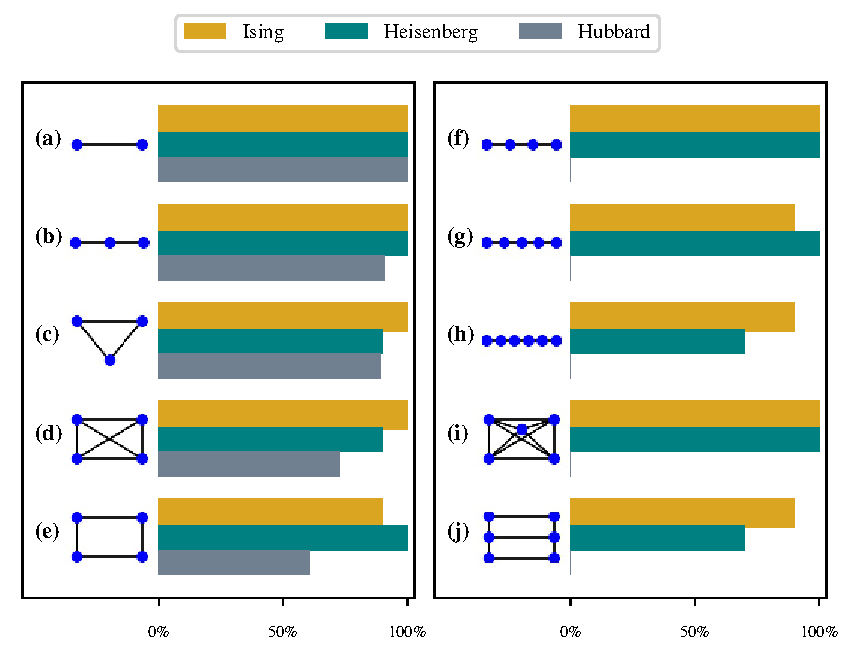
\includegraphics{theoretical_study/figures/lattices/lattice_successes_two_column.pdf}
    \end{center}
    \caption[\gls{qmla} Success rates for lattices]{
        Rates of success for \gls{qmla} under various conditions. 
        Each lattice is set as the true model $\ho$ for ten independent instances. 
        In each instance, the \gls{es} considers the available lattices 
            (\textbf{a-j} for Ising and Heisenberg cases and \textbf{a-e} for the Hubbard case), 
            and selects a champion model $\hp$ as that most consistent with data generated by $\ho$. 
        The figure displays the rate at which each lattice is correctly identified as $\ho$
            under standard Ising, Heisenberg and Hubbard formalisms. 
        \figtableref
    }
    \label{fig:lattice_success_rates}
\end{figure}    


    \chapter{Black box quantum systems}\label{chapter:black_box}
        \input{theoretical_study/black_box.tex}
    \chapter{Genetic algorithms}\label{chapter:ga}
        \glsresetall
The \gls{qmla} framework lends itself easily to the family of optimsation techniques called \emph{evolutionary algorithms}, 
    where individuals, sampled from a population of candidates, are considered as solutions to the given problem.
Candidates are batched in \emph{generations},
    such that iterative generations aim to efficiently search the available population
    by mimicing biological evolutionary mechanisms \cite{back1996evolutionary}. 
In particular, we develop an \gls{es} which incorporates a \gls{ga} in the construction of models;
    \glspl{ga} are a subset of evolutionary algorithms where candidate solutions are expressed as 
    strings of numbers representing some configuration of the system of interest \cite{holland1992adaptation}.
We describe the concepts of \glspl{ga} in \cref{sec:genetic_algorithms}, 
    so we begin this chapter by describing the adaptations which allow us to build a \gls{ges} within \gls{qmla}. 
\par 

\section{Adaptation to QMLA framework}\label{sec:ga_adaptation_to_qmla}
Unlike the generic aspects of \glspl{ga} described in \cref{sec:genetic_algorithms}, 
    in the context of \gls{qmla}, we must deviate from default mechanisms. 
The overarching goal of \gls{qmla} --
    to characterise some black box quantum system, \gls{q} --
    proceeds by designing and performing experiments upon \gls{q} which enable us to improve 
    the modelling of $\ho$. 
Nothing described so far provides a natural \gls{of}, upon which \glspl{ga} rely 
    to assess the suitability of candidates relative to contemporaries.
We can not assume knowledge of $\ho$ while generating candidates \glspl{model},
    so we can not simply invoke some loss function with respect to the target model, for example. 
Instead, we must devise schemes which exploit the knowledge we \emph{do} have about each candidate $\hj$, 
    which is the primary challenge in building an \gls{es} based on a \gls{ga}.  
We propose and discuss a number of options in \cref{sec:objective_functions}. 
\par 

Common to all proposed \glspl{of}, however, is that candidates should first be trained before evaluation, 
    so that their assessment is based on their actual power in describing \gls{q},  
    rather than some initial paramterisation which may not capture their potential. 
This is a tenet of \gls{qmla}: for each candidate $\hj ( \al_j )$, we use a subroutine to optimise $\al_j$;
    as in earlier applications of \gls{qmla}, for this study we rely on \gls{qhl} as the parameter optimisation subroutine. 
\par

Ultimately, the conceived role of a \gls{ga} within \gls{qmla} is to generate the sets of models to place 
    on successive branches\footnote{Branches in \gls{qmla} and generations of the \glsentrylong{ga} are equivalent here.} 
    of an \gls{et} as depicted in \cref{fig:qmla_overview}.
The apparatus within \gls{qmla} which facilitates novel model generation techniques is the \glsentryfull{es}.
Here we will design an \gls{es} which acts in cooperation with a \gls{ga}:
    the \gls{es} specifies that consolidation of a generation $\mu$ involve evaluating the \emph{fitness}, 
    $g_i$, of each candidate, $\hi$, via the chosen \gls{of}; 
    the \gls{ga} then maps $\{g_i\}$ of each $\hi \in \mu$ to a selection probability, 
    and composes new candidates via crossover, \cref{sec:reproduction}. 
Recall from \cref{sec:model_generation}, that we capture the space of available terms as $\termset$, 
    i.e. we list -- in advance -- the feasible terms which may be included in candidate models\footnotemark, 
    with $N_t = | \termset |$ the number of terms considered. 
\gls{qmla} is then an optimisation algorithm, attempting to find the set $\termset^{\prime}$
    which \emph{best} represents the true terms $\termset_0$.
Note, this does not require idenitifcation of the precise \gls{true model} to be successful, 
    as insight can be gained from approximate models which capture the physics of the target system. 
We introduce metrics for success in \cref{sec:f_score}. 
We recognise the limitations this structure imposes: we can only identify terms which were conceived in advance; 
    this may restrict \gls{qmla}'s applicability to entirely unknown systems, 
    where such a primitive set can not even be compiled.  
\footnotetext{
    Recall that models impose structure on sets of terms: $\hj = \al_j \cdot \vec{T}_j = \sum_{k \in \{j\}} \alpha_k \hat{t}_k$.
}    
\par 

The structure of the overall \gls{qmla} algorithm (recall \cref{fig:qmla_overview}) is unchanged.
In a \gls{ges}:
\begin{easylist}[itemize]
    & Branches: models are still grouped in branches, here called generations;
    & Training: models are still trained, again through \gls{qhl};
    & Consolidation: all models are evaluated according the the \gls{of} to be described in \cref{sec:objective_functions}, 
        so branches are consolidated by ranking models according to their fitness;
    & Spawning: new models are spawned through the \gls{ga} by selecting pairs of parents for crossover, 
        with the resultant offspring models probabilistically mutated. 
\end{easylist}
\par 

The design of any \gls{es} centres on the implementation of the 
    \ttt{generate\_models} subroutine -- we summarise the \gls{ges}'s method in \cref{alg:ga_generate_models}. 
We can restate the informal description of \glspl{ga}\footnotemark, now in the context of \gls{qmla}, as
\footnotetext{First stated on \cpageref{mark:informal_ga}.}

\begin{easylist}[enumerate]
    \ListProperties(Numbers2=l, Numbers3=r)
    & Sample $N_m$ models from $\population$ at random
    && this is the first generation, $\mu$. 
    & \label{qmla_ga:loop} Evaluate each model $\hj \in \mu$
    && train $\hj$ through \gls{qhl};
    && apply the \glsentrylong{of} to assign the model's fitness, $g_j$.
    & Map the fitnesses of each model, $\{g_j\}$, to selection probabilities for each model, $\{s_j\}$
    && e.g. by normalising the fitnesses, or by removing some poorly-performing models and then normalising. 
    & Generate the next generation of models
    && Reset $\mu = \{ \}$;
    && \label{qmla_ga:select} Select pairs of parents, $\h_{p_1}, \h_{p_2}$, from $\mu$
    &&& Each model's probability of being chosen is proportional to their $s_j$;
    && Cross over $\h_{p_1}, \h_{p_2}$ to produce children models, $\h_{c_1}, \h_{c_2}$
    &&& mutate $\h_{c_1}, \h_{c_2}$ according to some random probabilistic process;
    &&& $\mu \gets \mu \cup \{\h_{c_i} \}$, only if $\h_{c_i}$  is not already in $\mu$, 
        to ensure $N_m$ unique models are tested at each generation;
    && until $| \mu| = N_m$, iterate to step (\ref{qmla_ga:select}.
    & Until the $N_g^{th}$ generation is reached, iterate to step \ref{qmla_ga:loop}.
    & The strongest model on the final generation is deemed the approximation to the system, $\hp$. 
\end{easylist}



\par 

\subsection{Models as chromosomes}
We first need a mapping from models to chromosomes; 
    this is straightforward given the description of chromosomes as binary strings, 
    exemplified in \cref{sec:knapsack}. 
We assign a gene to every term in $\termset$, so that candidate models are succinctly represented by bit strings of length $N_t$. 
We give an example of the mapping between models and chromosomes in \cref{table:chromosome_example}.
Given that every model is contained in the space of bit strings spanned by $N_t$ bits, 
    we can say that there are a total of $2^{N_t}$ available models in the \gls{model space}. 


\begin{table}

    \renewcommand{\arraystretch}{2.0}
    \setlength{\tabcolsep}{5pt}

    \def\rowbox#1#2{%
        \smash{\color{#2}\fboxrule=1pt\relax\fboxsep=2pt\relax%
        \llap{\rlap{\fbox{\vphantom{0}\makebox[#1]{}}}~}}\ignorespaces
    }

    \definecolor{parentA}{HTML}{002bd8} % blue
    \definecolor{parentB}{HTML}{316c00} % green
    \definecolor{mutation}{HTML}{961f29} % red
    \newcommand\parentcolourA{parentA}
    \newcommand\parentcolourB{parentB}
    \newcommand\mutationcolour{mutation}

    % \newcommand\parentcolourA{blue}
    % \newcommand\parentcolourB{green}
    % \newcommand\mutationcolour{red}

    \newcommand\longrowboxlenth{185pt}
    \newcommand\shortrowboxlength{80pt}
    
    \begin{center}
    \begin{tabular}{ c  c | c  c  c  c  c  c } 
            \hline
        \multicolumn{2}{c|}{Model} & \multicolumn{6}{c}{Chromosome} \\
        & $\terms$ & $\hat{\sigma}_{(1,2)}^{x}$ & $\hat{\sigma}_{(1,2)}^{z}$ & $\hat{\sigma}_{(2,3)}^{y}$ 
            & $\hat{\sigma}_{(2,3)}^{x}$ & $\hat{\sigma}_{(2,3)}^{y}$ & $\hat{\sigma}_{(2,3)}^{x}$ 
            \\ 
        \hline
        \textcolor{\parentcolourA}{$\gamma_{p_1}$} & $\irow{ 
            \textcolor{\parentcolourA}{ \hat{\sigma}_{(1,2)}^{x}} 
            & \textcolor{\parentcolourA}{ \hat{\sigma}_{(1,2)}^{z}} 
            & \textcolor{\parentcolourA}{ \hat{\sigma}_{(2,3)}^{y}} 
        }$
        & \rowbox{\longrowboxlenth}{\parentcolourA} 1 & 0 & 1 & 0 & 1 & 0 \\
        \textcolor{\parentcolourB}{$\gamma_{p_2}$} & $\irow{ 
            \textcolor{\parentcolourB}{ \hat{\sigma}_{(1,2)}^{z}} 
            & \textcolor{\parentcolourB}{ \hat{\sigma}_{(2, 3)}^{y}} 
            & \textcolor{\parentcolourB}{ \hat{\sigma}_{(2,3)}^{z}} 
        }$
        & \rowbox{\longrowboxlenth}{\parentcolourB} 0 & 0 & 1 & 0 & 1 & 1 \\

        \hline
        $\gamma_{c_1}$ & $\irow{ 
            \textcolor{\parentcolourA}{ \hat{\sigma}_{(1,2)}^{x}} 
            & \textcolor{\parentcolourA}{ \hat{\sigma}_{(1,2)}^{z}} 
            % & \textcolor{\parentcolourB}{ \hat{\sigma}_{(2, 3)}^{x}} 
            & \textcolor{\parentcolourB}{ \hat{\sigma}_{(2, 3)}^{y}} 
            & \textcolor{\parentcolourB}{ \hat{\sigma}_{(2,3)}^{z}} 
        }$
        & \rowbox{\shortrowboxlength}{\parentcolourA} 1 & 0 & 1 & \rowbox{\shortrowboxlength}{\parentcolourB} 0 & 1 & 1 \\
        $\gamma_{c_2}$ & $\irow{ 
            \textcolor{\parentcolourA}{ \hat{\sigma}_{(1,2)}^{z}} 
            & \textcolor{\parentcolourB}{ \hat{\sigma}_{(2, 3)}^{y}} 
        }$
        & \rowbox{\shortrowboxlength}{\parentcolourB} 0 & 0 & 1 & \rowbox{\shortrowboxlength}{\parentcolourA} 0 & 1 & 0\\

        \hline

        $\gamma_{c_2}^{\prime}$ & $\irow{ 
            \textcolor{\parentcolourA}{ \hat{\sigma}_{(1,2)}^{z}} 
            & \textcolor{\mutationcolour}{ \hat{\sigma}_{(2, 3)}^{x}} 
            & \textcolor{\parentcolourB}{ \hat{\sigma}_{(2, 3)}^{y}} 
        }$
        & 0 & 0 & 1 & \rowbox{10pt}{\mutationcolour} 1 & 1 & 0\\
        \hline 
    \end{tabular}

    \caption[Mapping between QMLA's models and chromosomes used by a genetic algorithm]{
        Mapping between \gls{qmla}'s models and chromosomes used by a genetic algorithm. 
        Example shown for a three-qubit system with six possible terms, $\s_{i,j}^{w} = \s_i^w \s_j^w$. 
        Model terms are mapped to binary genes: 
            if the gene registers $1$ ($0$) then the corresponding term is (not) present in the model.
        The top two chromosomes are \emph{parents}, $\gamma_{p_1}=101010$ (blue) and $\gamma_{p_2}=001011$ (green):
            they are mixed to spawn new models. 
        We use a one--point cross over about the midpoint:
            the first half of $\gamma_{p_1}$ is mixed with the second half of $\gamma_{p_2}$ 
            to produce two new offspring chromosomes, $\{\gamma_{c_1}, \gamma_{c_2}$\}. 
        Mutation occurs probabilistically: each gene has a 25$\%$ chance of being mutated, e.g. a single gene (red) flipping from $0 \rightarrow 1$ to mutate $\gamma_{c_2}$ to $\gamma_{c_2}^{\prime}$.
        The next generation of the genetic algorithm will then include $\{\gamma_{c_1}, \gamma_{c_2}^{\prime}\}$ (assuming $\gamma_{c_1}$ does not mutate). 
        To generate $N_m$ models for each generation, $N_m/2$ parent couples are sampled from the previous generation and crossed over. 
    }
    \label{table:chromosome_example}
    \end{center}
\end{table}



\subsection{$F_1$-score}\label{sec:f_score}
\glsreset{tp}
\glsreset{tn}
\glsreset{fp}
\glsreset{fn}
We need a metric against which to evaluate models, and indeed the entire \gls{qmla} procedure. 
We can gauge the performance of \gls{qmla}'s model search by the quality of candidate models 
    produced at each generation, so we introduce a metric to act as proxy for model quality: 
    the $\fs$, denoted $f$. 
We define $\fs$ formally in this section, but in short, 
    $f \in \left(0, 1\right)$ indicates the degree to which $\hi$ captures the physics of the target system: 
    $f=0$ indicates that $\hi$ shares no terms with $\ho$, while $f=1$ is found uniquely for $\hi=\ho$. 
We defined $\fs$, as well as a number of metrics in the field of classification in \gls{ml}, in \cref{sec:performance_metrics};
    here we modify those definitions to align with the nomenclature of \gls{qmla}.
    
\par 

We emphasise that the goal of this work is to identify the \emph{model} which best describes 
    quantum systems, and not to improve on parameter-learning when given access to particular models, 
    since those already exist to a high standard \cite{wiebe2014qhlpra,bairey2019learning}. 
Therefore we can consider \gls{qmla} as a classification algorithm, 
    with the goal of classifying whether individual terms $\hat{t}$ from a set of available 
    terms $\termset = \{\hat{t}\}$ are helpful in describing data which is generated by $\ho$, 
    whose terms constitute $\termset_0$. 
Candidate models $\hi$ then have $\termset_i$.
We can assess $\hi$ using standard metrics used regularly in the \gls{ml} literature, 
    which simply count the number of terms identified correctly and incorrectly:
\begin{easylist}[itemize]
    & \gls{tp}: number of terms in $\To$ which are in $\Ti$
    & \gls{tn}: number of terms not in $\To$ which are also not in $\Ti$
    & \gls{fp}: number of terms in $\Ti$ which are not in $\To$
    & \gls{fn}: number of terms in $\To$ which are not in $\Ti$.
\end{easylist}
\par 

\noindent These concepts -- shown in \cref{fig:classification_eg} -- allow us to define 

\begin{easylist}
    & \emph{precision}: how precisely does $\hi$ capture $\ho$,
    i.e. if a term is included in $\Ti$ how likely it is to actually be in $\To$, Eqn \ref{eqn:precision};
    & \emph{sensitivity}: how sensitive is $\hi$ to $\ho$, 
    i.e. if a term is actually in $\To$, how likely $\Ti$ is to include it, Eqn. \ref{eqn:sensitivity}.
\end{easylist}

\begin{subequations}
    \begin{equation}
        \label{eqn:precision}
        \text{precision} = \frac{\textrm{TP}}{\textrm{TP} + \textrm{FP}}
    \end{equation}
       
    \begin{equation}
        \label{eqn:sensitivity}
        \text{sensitivity} = \frac{\textrm{TP}}{\textrm{TP} + \textrm{FN}}
    \end{equation}
\end{subequations}

Informally, precision prioritises that predicted terms are correct, 
    while sensitivity prioritises that true terms are identified. 
In practice, it is important to balance these considerations. 
$F_{\beta}$-score (\cref{eqn:f_beta}) is a measure which balances these,
    with weighting $\beta$ in favour of sensitivity.
In particular, $F_1$-score considers precision and sensitivity as equally important:
\begin{equation}
    \label{eqn:f1_score}
    F_1 = \frac{
        2\times (\textrm{precision})\times(\textrm{sensitivity})
    }{
        (\textrm{precision} + \textrm{sensitivity})
    } = \frac{\textrm{TP}}{\textrm{TP} + \frac{1}{2}(\textrm{FP} + \textrm{FN})} =: f.
\end{equation}
We give an example of these quantities in \cref{fig:classification_eg}, 
    where $\textrm{TP}=3, \textrm{TN}=4, \textrm{FP}=1, \textrm{FN}=2$, giving $\textrm{precision} = \nicefrac{3}{4}$ 
    and $\textrm{sensitivity} = \nicefrac{3}{5}$, 
    with a final $f = 0.67$, i.e. $f$ is the average of the indicators of model quality we care about. 
\par 

We adopt \fs \ as an indication of model quality because we are concerned both with precision and sensitivity
    of the models \gls{qmla} predicts as representations of \gls{q}. 
We can use \fs \ to measure the success of the algorithm,
    by recording $f$ for all models in all generations, allowing us to 
    see whether or not the approximation of the system is improving on average. 
Of course in realistic cases we can not assume knoweldge of $\termset_o$ and therefore cannot compute 
    $\fs$, but it is a useful tool in the development of the \gls{ges} itself, 
    or in cases where $\ho$ is known, such as when the target system is simualated, e.g. in the case of device calibration.
Our search for an effective \gls{of} can then be guided by seeking the 
    method which most strongly improves the average \fs \ in test-cases.
We will not use $\fs$ within the algorithm\footnote{Except for meta-analysis in \cref{sec:hyperparameter}}, 
    i.e. to inform any steps taken by \gls{qmla}, but simply to assess its performance independently.

\begin{figure}
    \begin{center}
        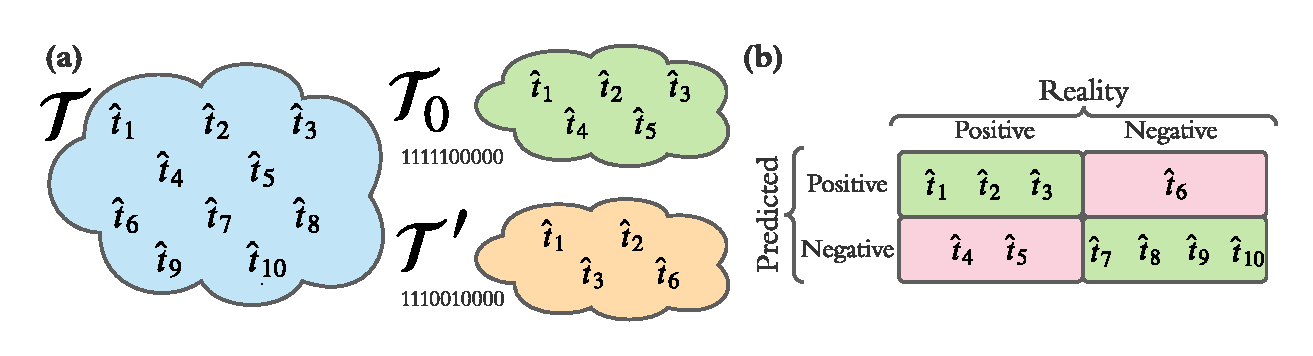
\includegraphics[width=\textwidth]{theoretical_study/figures/classication_example.pdf}
    \end{center}
    \caption[Classification concepts]{
        Concepts used for classification. 
        \textbf{a}, the set of available terms $\termset$ containing individual terms $\hat{t}_1$ to $\hat{t}_{10}$. 
        The \gls{true model} $\ho$ is constructed from the set $\termset_0$. 
        Suppose a candidate $\hp$ has the set $\termset^{\prime}$. 
        \textbf{b}, the confusion matrix for $\hp$. Correctly classified terms are \glsentrylong{tp} and \glsentrylong{tn} (green), 
            and incorrectly classified terms are \glsentrylong{fp} and \glsentrylong{tn} (red). 
    }
    \label{fig:classification_eg}
\end{figure}

\begin{algorithm}
    \caption{\gls{es} subroutine: \ttt{generate\_models} via genetic algorithm}
    \label{alg:ga_generate_models}
    \DontPrintSemicolon
    \KwIn{ $\nu$ \tcp*[1]{information about models considered to date}}\
    \KwIn{ $t$ \tcp*[1]{truncation rate}}\;
    \KwIn{ $g(\hi)$ \tcp*[1]{objective function that can act on any model $\hi$}}\;

    \KwOut{$\mathbb{H}$ \tcp*[1]{set of models}}\;
    
    $ N_m = \left| \nu \right| $ \tcp*[1]{number of models}

    \For{$\hi \in \nu$}{
       $g_i \gets g(\hi)$ \tcp*[1]{model fitness via objective function}
    }\;
    $r \gets $ \ttt{rank($\{ g_i \}$)} \tcp*[1]{rank models by their fitness}
    $\mathbb{H}_t \gets $ \ttt{truncate($r, N_m\times t$)} \tcp*[1]{truncate models by rank: only keep $N_m \times t$}
    $ s \gets $ \ttt{normalise($\{g_i\}$)} $\forall \hi \in \mathbb{H}_t$ \tcp*[1]{normalise remaining models' fitnesses}

    $\mathbb{H} = \{\}$ \tcp*[1]{new batch of chromosomes/models}

    \While{ $\left| \mathbb{H} \right| < N_m$ }{
        $p_1, p_2 = $ \ttt{roulette($s$)} \tcp*[1]{use $s$ to select two parents via roulette selection}
    
        $c_1, c_2$ = \ttt{crossover($p_1, p_2$)} \tcp*[1]{produce offspring models}

        $c_1, c_2$ = \ttt{mutate($c_1, c_2$)} \tcp*[1]{probabilistically mutate}

        $\mathbb{H} \gets \mathbb{H} \cup \{ c_1, c_2 \} $ \tcp*[1]{add new models to batch}

    }\;

    % \ttt{roulette($s$)}

    return $\mathbb{H}$ 

\end{algorithm}


\subsubsection{Distinguishing $\fs$ through Bayes factors}\label{sec:bf_by_f_score}
We have so far relied on \gls{bf} as the means by which to distinguish models' 
    ability to explain data from \gls{q}. 
We conjecture that models of higher $\fs$ are usually statistically better at predicting dynamics of \gls{q}
    than those of lower $\fs$, and therefore \glspl{bf} will favour models of higher $\fs$;
Verifying this hypothesis will allow us to incorporate statistical tools into the design of \glspl{of};
    we can perform straightforward tests training models of equally spaced $\fs$, and computing \glsentryshort{bf} between all pairs.
\par 

In \cref{fig:bf_by_fscore}, we show the relationships between $\fs$ and \gls{bf} for various conditions. 
Firstly, under a standard training regime with full \gls{bf} comparisons between all pairs, 
    we see that in most cases, the model with higher $\fs$ is favoured by \gls{bf}.
In \cref{fig:bf_by_fscore}b, we run a complete model training subroutine, but compute the \gls{bf} based on fewer experiments and particles 
    (retaining a fraction $\Np^{\prime} = 0.2\Np, \ \Ne^{\prime} = 0.2\Ne$ for comparisons).
This verifies an earlier claim from \cref{sec:experiments_for_bf}: 
    although the strength of evidence is weaker given reduced \gls{bf} resources, 
    the direction of the evidence is usually the same, i.e. the insight is indicative of the true physics, 
    so we can save considerable compute time by trusting these restricted \gls{bf} calculations. 
On the other extreme, we see in \cref{fig:bf_by_fscore}\textbf{c}, where models are trained with
    -- and \glspl{bf} based upon -- even greater resources than \cref{fig:bf_by_fscore}\textbf{a}, we see a similar effect: 
    adding resources strengthens the evidence, but does not fundamentally change the outlook. 
Finally, in addition to reducing the resources used per \gls{bf} calculation, 
    we reduce the number of comparisons computed in \cref{fig:bf_by_fscore}\textbf{d}, 
    as permitted when rating models according to the \gls{of} to be described in \cref{sec:elo}, 
    or similar measures which can yield fitnesses from reduced data. 
Essentially we can see that the insight is largely the same 
    from the most and least expensive training/comparison strategies, 
    and by leveraging the available evidence (\cref{fig:bf_by_fscore}\textbf{d}), 
    rather than brute-force computing as much evidence as possible (\cref{fig:bf_by_fscore}\textbf{a}), 
    we can achieve similar results. 
Note that the time saving reported between full and partial connectivity between models scales with $N_m$: 
    here, with $N_m=10$, the former computes 45 \glspl{bf}, while the latter computes 17;
    for $N_m=60$, as used in full instances/runs presented in this chapter, these rise to 600 and 1770 respectively, 
    so the benefit of the latter scheme is amplified. 
% This saving depends on the user's choice of graph connectivity, see \cref{sec:elo_graph}, 
%     though is typically a factor between 2-3;
%     in general, though, assuming we can reduce the resources used within the \gls{bf}, 
%     this phase is considerably less cumbersome than the model training itself, so 
%     it is feasible to compute all available \glspl{bf} to inform the \gls{bfeer}.

\begin{figure}
    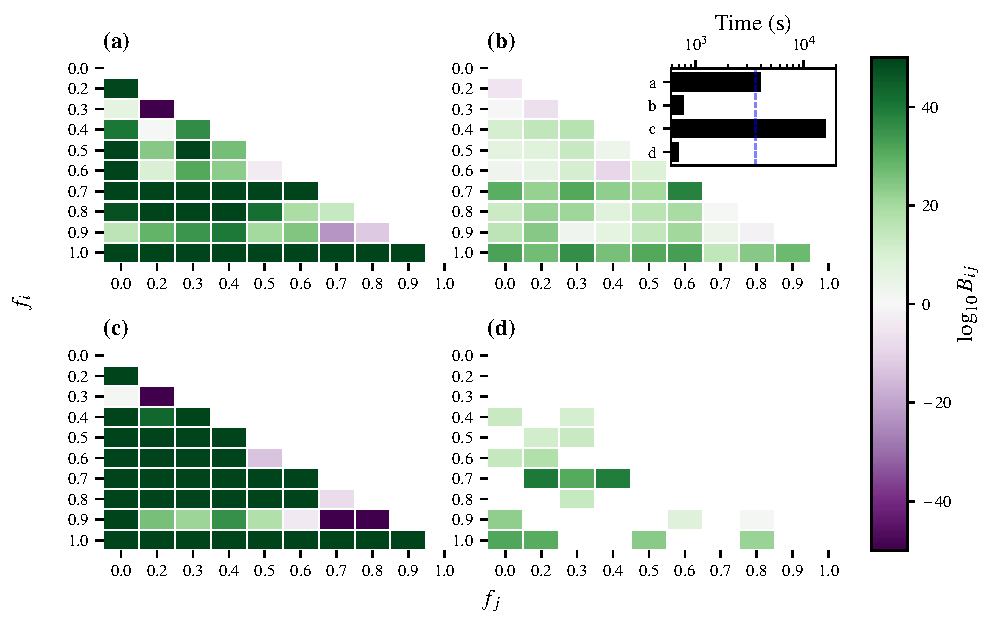
\includegraphics{theoretical_study/figures/bayes_factors_by_f_scores.pdf}
    \caption[\glsentrylong{bf} by $\fs$]{
        Pairwise \glsentrylong{bf}, $\bij$, by $\fs$ of candidates $\hi$ ($f_i$ on the $y$-axis) 
        and $\hj$ ($f_j$ on the $x$-axis).
        $\log_{10}\bij > 0 \ (<0)$, green (purple), indicates statistical evidence that $\hi$ ($\hj$) 
        is the better model with respect to the observed data.
        Visualisation is curtailed to $\log_{10} \bij = \pm 50$. 
        \textbf{a}, Models are trained with $\Ne=500, \Np=2500$,
            and all available data is used in the calculation of \glspl{bf}. 
        \textbf{b}, $\Ne=500, \Np=2500$ using only a fraction (0.2) of experiments/particles for \gls{bf} calculations. 
        \textbf{c}, $\Ne=1000, \Np=5000$, using all available data in the calculation of \glspl{bf}. 
        \textbf{d}, $\Ne=500, \Np=2500$, comparing only a subset of pairs of models through \glspl{bf}, 
            and using only a fraction ($0.2$) of experiments/particles for those calculations. 
            This pairwise comparison strategy is used for the \gls{of} in \cref{sec:elo}. 
        \textbf{Inset}, timings for each approach in seconds, with $t=1\textrm{hr}$ marked vertically in blue. 
        \figtableref
    }
    \label{fig:bf_by_fscore}
\end{figure}


\subsection{Hyperparameter search}
\label{sec:hyperparameter}
\begin{figure}
    \begin{center}
        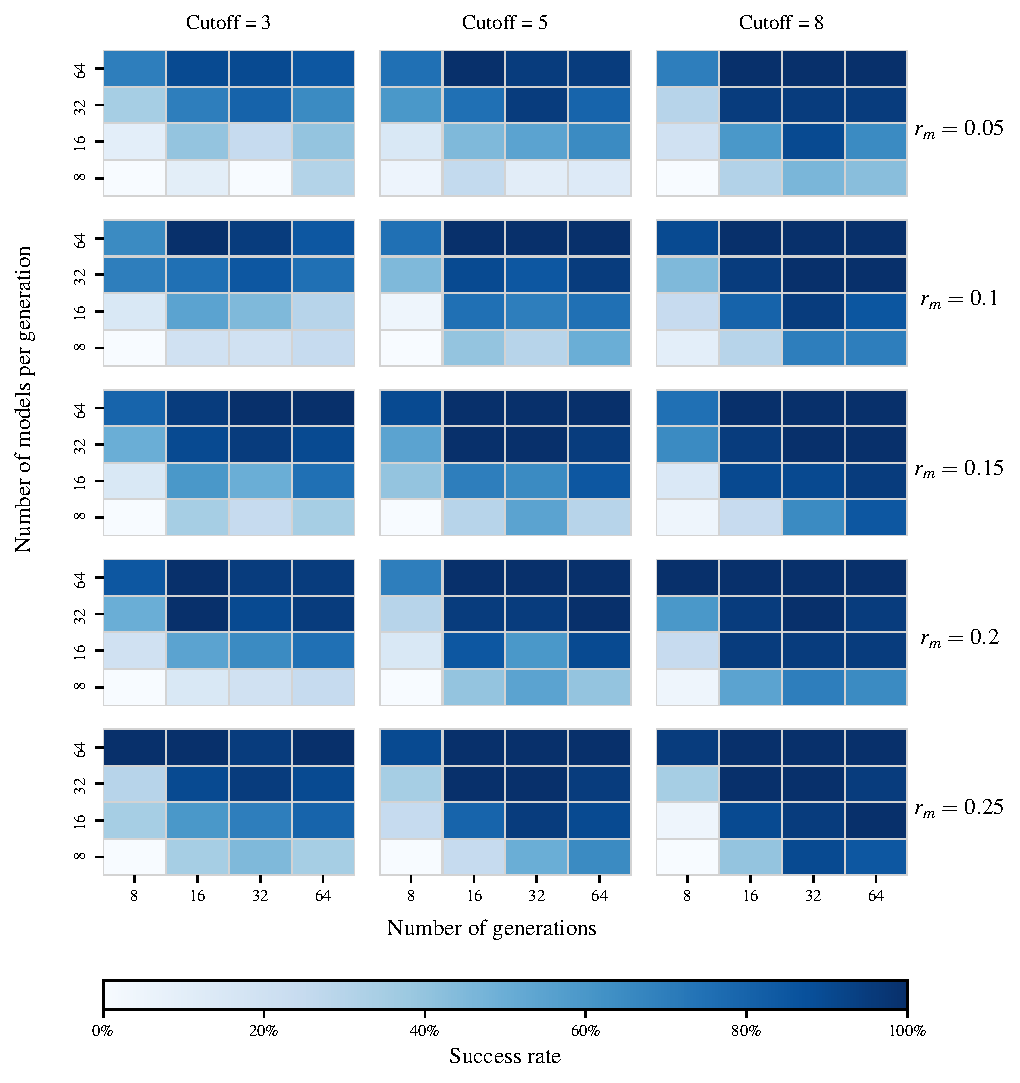
\includegraphics{theoretical_study/figures/gen_alg_param_sweep.pdf}
    \end{center}
    \caption[Genetic algorithm parameter sweep]{
        Genetic algorithm parameter sweep.
        Each subplot shows the success rates for varying numbers of generations, $N_G \in \{8, 16, 32, 64\}$, 
        and numbers of models per generation, $N_m \in \{8, 16, 32, 64\}$. 
        A subplot is generated for ranges of the mutation rate, $r_m$ and the number of 
        generations for which the elite model is unchanged after which the \gls{ga} is cut off.
        \figtableref 
    }
    \label{fig:ga_param_sweep}
\end{figure}

Firstly we will validate our reasoning that $\fs$ is a sensible figure of merit, 
    by directly invoking it as the \glsentrylong{of}. 
That is, we first implement a \gls{ga}, using the mapping between models and chromosomes outlined above,
    where we fix the numbers of sites $d=4$, and assume full connectivity between the sites, with $x-$, $y-$ and $z-$ couplings available,
        such that there are $N_t = 3 \times {4 \choose 2} = 18$ terms in $\termset$, so that the total population is of size $2^{18}$ chromosomes.
We can then sweep over the \gls{ga} \glspl{hyperparameter} to find a suitable configuration:
    in \cref{fig:ga_param_sweep} we show how the choice of parameters affect the success rate of preciesly identifying the 
    target chromosome, which is chosen at random for each instance, and we run 20 \glspl{instance} of each configuration. 
The studied hyperparameters\footnotemark \ are
\begin{easylist}[enumerate]
    \ListProperties(Numbers=r)
    & number of generations;
    & number of models per generation;
    & mutation rate, $r_m$;
    & number of generations for which a candidate must reign as the strongest observed, before the search terminates, the \emph{cutoff}. 
\end{easylist}
\footnotetext{  
    These and further \glspl{hyperparameter} can be swept using code within the \gls{qmla} codebase, 
    in the directory \ttt{scripts/genetic\_alg\_param\_sweep}.  
}
Naturally, we expect that running for more generations with more models per generation will result in a more effective search in the model space, 
    having examined $N_gN_m$ models. 
We must also consider, however, that -- in realistic cases of \gls{qmla} -- the total computation time scales dramatically with these parameters, 
    since training and comparing models are expensive subroutines. 
Our goal is therefore to identify the set of \glspl{hyperparameter} which best searches the \gls{model space} 
    while demanding the lowest $N_g, N_m$.  
We see that, unsurprisingly, the \gls{ga} performs poorly when run with few resources, 
    but broadly the performances are similiar provided it is run with sufficient resources.
We can bound the parameters $r_m \geq 0.1, \textrm{cutoff} \geq 5, N_m \geq 16, N_g \geq 16$ to ensure a reasonable 
    search through the model space, without having to consider a prohibitive number of models. 
We must bear in mind, however, that this parameter sweep refers only to the trivial case where 
    the $\fs$ is used as the \gls{of}, so we do not expect such high success rates in realistic cases.

\section{Objective functions}\label{sec:objective_functions}
\glsreset{of}
We have alluded to the central probelm in building a \gls{ga} into \gls{qmla}:
    how to evaluate trained candidate models in the absence of a natural \gls{of}. 
In \crefrange{sec:inverse_ll}{sec:elo} we will propose and analyse a number of potential \glspl{of}, 
    some of which will underlie later studies in this thesis. 
We conclude this study by comparing the proposed \glspl{of} and selecting one for consideration in the remainder of this chapter;
    readers interested in the final application may prefer to skip to \cref{sec:obj_fnc_selection}.
\par 
We will show how each \gls{of} computes a fitness, $g_i$, for candidate models, $\hi$.
For examples of each, we group together some demonstrative values in \cref{table:objective_functions}.
For each $\hi$, we may refer to 
\begin{easylist}[itemize]\label{list:obj_fnc_terms}
    & $\tll_i$, \glsentryfull{tltl},  introduced in \cref{sec:total_log_total_likelihood};
    & $k_i$, the model's cardinality, i.e. number of terms in its parameterisation;
    & $\expset_i$, the bespoke set of experiments composed by the \glsentrylong{edh} (\cref{sec:heuristic}) solely for trainng $\hi$;
    & $n = |\expset_i|$, the number of samples (datapoints) used in trainng $\hi$. 
\end{easylist}
In \cref{table:objective_functions}, 
    we consider six randomly generated exemplary models 
    -- of varying quality with respect to the target, $\ho$, listed in \cref{eqn:obj_fnc_eg_models} -- 
    to demonstrate each \gls{of}'s outcomes.

\renewcommand{\arraystretch}{1.25} % space between rows
\setlength{\tabcolsep}{2pt}

\begin{equation}
    \label{eqn:obj_fnc_eg_models}
    \begin{align}
        \hat{H}_0 \ &= \ \s_{(1, 2)}^{z}\s_{(1, 3)}^{z}\s_{(2, 3)}^{z}\s_{(2, 5)}^{z}\s_{(3, 5)}^{z};\\
        \hat{H}_a \ &= \ \s_{(1, 5)}^{z}\s_{(3, 4)}^{z}\s_{(4, 5)}^{z}; \\
        \hat{H}_b \ &= \ \s_{(1, 4)}^{z}\s_{(1, 5)}^{z}\s_{(2, 5)}^{z}\s_{(3, 4)}^{z}; \\
        \hat{H}_c \ &= \ \s_{(1, 2)}^{z}\s_{(1, 5)}^{z}\s_{(2, 4)}^{z}\s_{(2, 5)}^{z}\s_{(4, 5)}^{z}; \\
        \hat{H}_d \ &= \ \s_{(1, 3)}^{z}\s_{(1, 4)}^{z}\s_{(1, 5)}^{z}\s_{(2, 4)}^{z}\s_{(2, 5)}^{z}\s_{(3, 4)}^{z}\s_{(3, 5)}^{z}; \\
        \hat{H}_e \ &= \ \s_{(1, 2)}^{z}\s_{(1, 3)}^{z}\s_{(1, 5)}^{z}\s_{(2, 3)}^{z}\s_{(2, 5)}^{z}\s_{(4, 5)}^{z}; \\
        \hat{H}_f \ &= \ \s_{(1, 2)}^{z}\s_{(1, 3)}^{z}\s_{(2, 3)}^{z}\s_{(2, 4)}^{z}\s_{(2, 5)}^{z}\s_{(3, 4)}^{z}\s_{(3, 5)}^{z}. \\
    \end{align}
\end{equation}

\begin{table}    
    \begin{tabular}{|cc|c|c|c|c|c|c|}
\hline
          &      &                              $\hat{H}_a$ &                              $\hat{H}_b$ &                              $\hat{H}_c$ &                              $\hat{H}_d$ &                              $\hat{H}_e$ &                              $\hat{H}_f$ \\
Method &  &                                          &                                          &                                          &                                          &                                          &                                          \\

          & $F_1$ &                                    $0.0$ &                                    $0.2$ &                                    $0.4$ &                                    $0.5$ &                                    $0.7$ &                                    $0.8$ \\
          & $k$ &                                        3 &                                        4 &                                        5 &                                        7 &                                        6 &                                        7 \\
          & $\overline{l_e}$ &                          $0.86 \pm 0.29$ &                          $0.84 \pm 0.29$ &                          $0.77 \pm 0.27$ &                          $0.78 \pm 0.29$ &                          $0.79 \pm 0.26$ &                          $0.79 \pm 0.26$ \\
          & $\tll_i$ &                                     -143 &                                     -152 &                                     -131 &                                     -150 &                                     -125 &                                     -124 \\
\hline \multirow{2}{*}{Inverse log-likelihood} & $g_i^L$ &                                  0.00698 &                                  0.00659 &                                  0.00766 &                                  0.00669 &                                  0.00803 &                                  0.00804 \\
          & $\%$ &                                       23 &                                        0 &                                       25 &                                        0 &                                       26 &                                       26 \\
\cline{1-8}
\hline \multirow{5}{*}{Akaike Info Criterion} & AIC &                                      293 &                                      311 &                                      271 &                                      313 &                                      261 &                                      263 \\
          & AICc &                                      293 &                                      312 &                                      272 &                                      314 &                                      262 &                                      264 \\
          & $w_i^A$ &                                 1.81e-07 &                                  1.4e-11 &                                  0.00724 &                                 4.15e-12 &                                        1 &                                    0.334 \\
          & $g_i^A$ &                                 1.17e-05 &                                 1.03e-05 &                                 1.35e-05 &                                 1.01e-05 &                                 1.46e-05 &                                 1.43e-05 \\
          & $\%$ &                                       22 &                                        0 &                                       25 &                                        0 &                                       27 &                                       26 \\
\cline{1-8}
\hline \multirow{4}{*}{Bayesian Info Criterion} & BIC &                                      301 &                                      322 &                                      284 &                                      331 &                                      277 &                                      281 \\
          & w_i^B &                                 5.49e-66 &                                 1.26e-70 &                                 1.97e-62 &                                 1.11e-72 &                                 8.43e-61 &                                 8.95e-62 \\
          & g_i^B &                                 1.11e-05 &                                 9.65e-06 &                                 1.24e-05 &                                 9.11e-06 &                                 1.31e-05 &                                 1.27e-05 \\
          & $\%$ &                                       23 &                                        0 &                                       25 &                                        0 &                                       27 &                                       26 \\
\cline{1-8}
\hline \multirow{2}{*}{Bayes factor points} & g_i^p &                                        0 &                                        2 &                                        3 &                                        2 &                                        3 &                                        5 \\
          & $\%$ &                                        0 &                                       13 &                                       20 &                                       13 &                                       20 &                                       33 \\
\cline{1-8}
\hline \multirow{3}{*}{Ranking points} & Ranking &                                        6 &                                        5 &                                        2 &                                        4 &                                        3 &                                        1 \\
          & g_i^R &                                        0 &                                        0 &                                      0.3 &                                      0.1 &                                      0.2 &                                      0.4 \\
          & $\%$ &                                        0 &                                        0 &                                       30 &                                       10 &                                       20 &                                       40 \\
\cline{1-8}
\hline \multirow{3}{*}{Elo rating} & Rating &                                      909 &                                      944 &                                     1042 &                                     1007 &                                     1011 &                                     1084 \\
          & g_i^E &                                        0 &                                       35 &                                      133 &                                       98 &                                      102 &                                      175 \\
          & $\%$ &                                        0 &                                        0 &                                       26 &                                       19 &                                       20 &                                       34 \\
\cline{1-8}
\hline \multirow{3}{*}{Residuals} & mean$\{\tilde{r_p^e}\}$ &                                    0.132 &                                    0.146 &                                    0.114 &                                    0.138 &                                   0.0858 &                                   0.0715 \\
          & g_i^r &                                    0.753 &                                    0.729 &                                    0.785 &                                    0.743 &                                    0.836 &                                    0.862 \\
          & $\%$ &                                       23 &                                        0 &                                       24 &                                        0 &                                       26 &                                       27 \\
\hline
\end{tabular}
 % TODO fix latex errors in table
    \caption[Objective function examples]{
        Examples of how each objective function, $g$ as described in \cref{sec:inverse_ll} to \cref{sec:elo},
            assign selection probability (denoted \%) to the same set of candidate models, $\{\hi\}$ listed in \cref{eqn:obj_fnc_eg_models}, 
            when attempting to learn data from $\ho$. 
        Intermediate quantities, e.g. $w_i^A$, $g_i^p$ are described in the section of the main text describing the corresponding \gls{of}.
        For each model we first summarise its
            $\fs$ (\cref{eqn:f1_score}),
            number of terms $k$,
            median  \gls{likelihood} $\overline{l_e}$ (\cref{eqn:log_likelihood}),     
            and \gls{tltl} $\tll_{i}$ (\cref{eqn:log_total_likelihood}), 
        We use $n=250$ samples, i.e. $\tll_{i}$ is a sum of $n$ \glspl{likelihood} .  
        The set of models is truncated so that only the strongest four are assigned selection probability. 
    }
    \label{table:objective_functions}
\end{table}

\subsection{Inverse log-likelihood}\label{sec:inverse_ll}
$\tll_{i}$, defined in \cref{eqn:log_total_likelihood}, can be thought of as a measure of the success of a given model at explaining data from any set of experiments, $\expset$. 
This can be immediately interpreted as an \gls{of}, provided each candidate model 
    computes a meaningful \gls{tltl}, requiring that they are all based on the same set of experiments, $\expset_v$,
    which are designed explicitly for the purpose of model evaluation. 
\par 

\gls{tltl} are negative and the strongest model has lowest $\lvert \tll_{i} \rvert$ (or highest $\tll_{i}$ overall),
    so the corresponding \gls{of} for candidate $\hi$ is 
\begin{equation}
    \label{eqn:obj_log_likelihood}
    g_i^{L} = \frac{-1}{\tll_{i}}.
\end{equation}

In our tests, Eqn. \ref{eqn:obj_log_likelihood} is found to be too generous to poor models, 
    assigning them non-negligible probability. 
Its primary flaw, however, is its reliance on $\expset_v$: 
    in order that the \gls{tltl} is significant, it must be based on meaningful experiments, 
    the design of which can not be gauranteed in advance, or at least risks introducing strong bias
    towards some models. 

\subsection{Akaike information criterion}\label{sec:akaike_info_criterion}
A common metric in the general field of model selection is \gls{aic} \cite{dr2002model}.
Incorporating \gls{tltl}, 
    \gls{aic} objectively quantifies how well a given model accounts for data from the target system,
    and explicitly punishes models which use extraneous parameters by incurring a penalty on $k_i$. 
\gls{aic} is given by 
\begin{equation}
    \label{eqn:aic}
    AIC_i = 2k_i - 2 \tll_{i}.
\end{equation}

In practice we use a slightly modified form of Eqn. \ref{eqn:aic} which
    corrects for the number of samples $n=\lvert\expset_i\rvert$, 
    called the \gls{aicc}, 
\begin{equation}
    \label{eqn:aicc}
    AICC_i = AIC_i + 2k_i \frac{k_i+1}{n-k_i-1}. 
\end{equation}

Model selection from a set of candidates occurs simply by selecting the model with lowest $AICC$.
Following \cite{dr2002model}, by using Eqn. \ref{eqn:aicc} as a measure of \emph{relative likelihood}
    we retrieve selection probability via
    the \emph{Akaike weights},
\begin{equation}
    \label{eqn:akaike_weights}
    w_i^A = \exp \left( \frac{{AICC_{\textrm{min}} - AICC_i}}{2} \right), 
\end{equation}
    where $AICC_{\textrm{min}} = \min_{i}\{ AICC_i\}$.

Akaike weights impose quite strong penalties 
    on models which do not explain the data well, 
    but also punish models with extra parameters, i.e. overfitting models, 
    effectively searching for the strongest and simplest model simultaneously.
The level of punishment for poorly performing models is likely too drastic: 
    very few models will be in a range sufficiently close to $AICC_{\textrm{min}}$ 
    to receive a meaningful Akaike weight, 
    suppressing diversity in the model population.
    Indeed, we can see from Table \ref{table:objective_functions} that this results in most 
    models being assigned negligible weight, which is not useful for parent selection. 
Instead we compute a straightforward quantity related to \gls{aic},
\begin{equation}
    \label{eqn:akaike_fitness}
    g_i^{A} = \left(\frac{1}{AICc_i}\right)^2,
\end{equation}
    where we square the inverse \gls{aicc} to amplify the difference in quality between models, 
    such that stronger models are rewarded.

\par 

\subsection{Bayesian information criterion}\label{sec:bayes_info_criterion}
Related to the concept of \gls{aic} (Eqn. \ref{eqn:aic}), is that of \gls{bic}, 
\begin{equation}
    \label{eqn:bic}
    BIC_i = k_i \ ln(n_i) - 2 \tll_{i},
\end{equation}
    where $k_i, n_i$ and $\tll_i$ are as defined on \cpageref{list:obj_fnc_terms}.
    % where $k, \tll_{i}$ are as defined above and $n$ is the number of samples.
Analagously to Akaike weights, 
    \emph{Bayes weights} as proposed in \S7.7 of \cite{friedman2001elements}, are given by

\begin{equation}
    w_i^B = \exp\left( - \frac{BIC_i}{2}  \right).
\end{equation}

\gls{bic} is harsher than \gls{aic} in its punishment of models' cardinality $k_i$, 
    demanding substantial statistical justification for the inclusion of more parameters. 
Again, this may be overly cumbersome for our use case:
    with such a relatively small number of parameters, 
    the punishment is disproportionate.
As with Akaike weights, rather than using Bayes weights directly, 
    we opt for an \gls{of} related to them, 
\begin{equation}
    \label{eqn:bic_fitness}
    g_i^B = \left( \frac{1}{BIC_i}\right)^2.
\end{equation}
    

\subsection{Bayes factor points}\label{sec:bf_points}
A cornerstone of model selection within \gls{qmla} is the calculation of \glspl{bf} (see \cref{sec:bayes_factors}). 
We can compute the pairwise \gls{bf} between two candidate models, $\bij$, according to Eqn. \ref{eqn:bf_succinct}.
$\bij$ can be based on some evaluation dataset, $\expset_v$, but can also be calculated from $\expset_i \cup \expset_j$: 
    this is a strong advantage since the resulting insight (Eqn. \ref{eqn:bf_cases}) is based on 
    experiments which were bespoke to both $\hi, \hj$. 
As such we can be confident that this insight accurately points us to the stronger of two candidate models. 
\par 

We can utilise this facility by computing the \gls{bf} between all 
    pairs of models in a set of $N_m$ candidates $\{\hi\}$, 
    i.e. compute ${N_m \choose 2}$ \gls{bf}s. 
Note that this is computationally expensive: 
    in order to train $\hi$ on $\expset_j$ requires a further $\lvert \expset_j \rvert$ experiments, 
    each requiring $N_P$ particles\footnote{Caveat the reduction in overhead outlined in \cref{sec:experiments_for_bf}.}, 
    where each particle corresponds to a unitary evolution and therefore the caluclation of a matrix exponential. 
The size of the \gls{model space} is then quite a heavy disadvantage: 
    examining $N_g$ generations requires $N_g \times {N_m \choose 2}$ \gls{bf} calculations for complete assessment. 
In the case where all pairwise \gls{bf} are performed, 
    we can assign a point to $\hi$ for every comparison in which it is deemed superior, according to \cref{eqn:bf_cases}.
\begin{equation}
    \label{eqn:bf_points}
    g_i^p = \sum_{j \in \mu} b_{ij}, \ \ \ \ b_{ij} = 
        \begin{cases}
            1, \ \ \ \ \bij > 1 \\
            0, \ \ \ \ \text{otherwise}.
        \end{cases}
\end{equation}
This is a straightforward mechanism, but is overly blunt
    because it does not account for the strength of the evidence
    in favour of each model. 
For example, a dominant model will receive only a slightly higher selection probability 
    than the second strongest, even if the difference between them was $\bij = 10^{100}$. 
Further, the unfavourable scaling make this an expensive method. 

\subsection{Ranking}\label{sec:bf_ranking}
Related to \cref{sec:bf_points}, we can rank models in a generation based on their number of \gls{bf} points.
\gls{bf} points are assigned as in Eqn. \ref{eqn:bf_points}, 
    but instead of corresponding directly to fitness, 
    we assign models a rank $R$, 
    i.e. the model with highest $g_i^p$ gets $R=1$, 
    and the model with $n^{th}$ highest $g_i^p$ gets $R=n$. 
Note here we truncate $\mu$, meaning we remove the worse-performing models and retain only $N_m^{\prime}$ models, 
    before calculating $R$, because computing $R$ using all $N_m$ models results in less distinct selection probabilities. 

\begin{equation}
    \label{eqn:ranking}
    g_i^R = \frac{N_m^{\prime}-R_i+1}{\sum\limits_{n=1}^{N^{\prime}_m} n},
\end{equation}
    where $R_i$ is the ranking of $\hi$ and $N_m^{\prime}$ is the number of models retained after truncation. 
\cref{eqn:ranking} has a similary effect to \cref{eqn:bf_points} but awards higher selection probability to 
    the strongest models. 
However, it too overlooks the nuanced perspective available through the total statistical evidence gathered by the series of \glspl{bf}. 

\subsection{Residuals}\label{sec:residuals}
Recall at each experiment, $N_P$ particles are compared against a single experimental datum, $d$. 
By definition, $d$ is the binary outcome of the measurement on \gls{q} under experimental conditions $e$.
That is, $d$ encodes the answer to the question: 
    after time $t$ under Hamiltonian evolution, did \gls{q} project onto 
    the basis we have labelled $\ket{d}$ (usually the same as the input \gls{probe} state $\ket{\psi}$)?
\par 
In practice we often have access to the complete \gls{likelihood}, 
    i.e. rather than a binary value, we have a number representing the probability that 
    \gls{q} will project on to $d=0$ for a given experiment $e$, $\Pr_Q(0 | e)$. 
The likelihood -- in this case equivalent to the expectation value -- 
    for \gls{q} is usually given by $\absval{ \bra{\psi} e^{-i\ho t} \ket{\psi} }^2$.
For consistency with QInfer \cite{qinfer-1_0} -- on which \gls{qmla}'s code base extends --
    we call the expectation value for the system $\Pr_Q(0)$;
    the same quantity can be computed for each particle, called $\Pr_p(0)$.
Likewise, we can simulate this quantity for each particle, $\Pr_p(0 | e)$. 
This allows us to calculate the \emph{residual} between the system and individual particles' \glspl{likelihood}, $r_p^e$; 
    we can hence compute the mean residual across all particles in a single experiment $r^e$:
\begin{align}
    \label{eqn:particle_residual}
    \begin{split}
    r_p^e & = \absval{ Pr_Q(0 | e) - Pr_p(0 | e) }  \\
    r^e &= \underset{p}{\text{mean}} \{r_p^e\}
    \end{split}
\end{align}
\par 

Residuals capture how closely the particle distribution reproduced the dynamics from \gls{q}:
    $r^{e}_{p} = 0$ indicates perfect preditiction, while $r^e_p=1$ is completely incorrect. 
We can therefore maximise the quantity $1-r$ to find the best model, 
    using the \gls{of}
\begin{equation}
    \label{eqn:residual_fitness}
    g^r_i = \lvert 1 - \underset{e \in \expset}{\text{mean}}\{ {r^e} \}\rvert^2.
\end{equation}
\par     
This \gls{of} can be thought of in frequentist terms 
    as similar to the residual sum of squares,
    although instead of summing the residual squares, we take the average to ensure $0 \leq r \leq 1$. 
$g_i^r$ encapsulates how well the candidate model reproduces a paticular set of dynamics from the target system, 
    as a proxy for how well that candidate describes the system. 
This is not always a safe figure of merit: 
    in most cases, we do not expect parameter learning to perfectly optimise $\al_i$. 
Reproduced dynamics alone can not capture the prospect that $\hi=\ho$, 
    but rather inform statistical measures such as \gls{bf} that allow us to make 
    qualified statements about the system. \par 

This \gls{of} provides a useful test for \gls{qmla}'s \gls{ga}:
    by simulating the case where parameters \emph{are} learned perfectly, 
    such that we know that $g_i^r$ truly represents the ability of $\hi$ to 
    simulate $\ho$, then this \gls{of} gaurantees to promote  the strongest models,
    especially given that $\hi=\ho \implies r_p^e=0 \ \forall \ \{e, p\}$. 
In realistic cases, however, the non-zero residuals -- even for 
    strong $\hi$ -- may arise from imperfectly learned parameters,
    rendering the usefulness of this \gls{of} uncertain. 
Finally, it does not account for the cardinality, $k_i$, of the candidate models,
    which all \gls{ml} protocols aim to avoid in general;
    this could result in favouring severely overfitting models in order to 
    gain marginal improvement in residuals.

\subsection{Bayes factor enhanced Elo-ratings}\label{sec:elo}
A popular tool for rating individual competitors in sports and games is the \emph{Elo rating} scheme, 
    e.g. used to rate chess players and soccer teams \cite{elo1978rating, fifa_elo}, 
    also finding application in the study of animal hierarchies \cite{neumann2011assessing}. 
Elo ratings allow for evaluating the relative quality of individuals 
    based on incomplete pairwise competitions, 
    e.g. despite two football teams having never played against each other before, 
    it is possible to quantify the difference in quality between those teams, 
    and therefore to predict a result in advance \cite{hvattum2010using}. 
There is a direct a parallel between these types of competitions and \gls{qmla}:
    we similarly have a pool of individual competitors (models), 
    which we can place in direct competition, 
    and quantify the comparitive outcome through \gls{bf}, 
    in order to determine the strongest. 

\par 
Elo ratings are transitive: given some interconnectivity in a generation, 
    we need not compare \emph{every} pair of models in order to 
    make meaningful claims about which are strongest;
    it is sufficient to perform a subset of comparisons, 
    ensuring each individual undergoes robust competition.
We can take advantage of this transitivity to reduce the combinatorial overhead 
    usually associated with computing bespoke \glspl{bf} between all models 
    (i.e. using their own training data $\expset_i$ instead of a generic 
    $\expset_v$).
In practice, we map $N_m$ models within a generation to vertices on a regular graph
    of degree $nicefrac{N_m}{3}$, i.e. each model is connected to $\nicefrac{N_m}{3}$ 
    other models within $\mu$. 
Models which share an edge then undergo \gls{bf} comparison. 
For example, with $N_m=60$ this leads to $600$ \gls{bf} calculations, 
    compared with $1770$ calculations in the fully connected graph. 
While every pair of models $(\hi, \hat{H}_{m})$ are not directly connected, 
    there is always a chain of length $l \leq l_{max}$ edges between them.
For $N_m=60$, we find $l_{max}=2$, 
    e.g. for $\hi, \hat{H}_k$ disconnected, there are comparisons $(\hi, \hj), (\hj \hat{H}_k)$. 
    
\par 

The Elo rating scheme is a nonlinear points transfer system, as follows: 
    upon creation, $\hi$ is assigned a rating $R_i$; 
    every comparison with a competitor $\hj$ results in $\bij$; 
    $R_i$ is updated according to the known strength of its competitor, $R_j$, 
    as well as the result $\bij$. 
The Elo update ensures that winning models are rewarded 
    for defeating another model, 
    but that the extent of that reward reflects the quality of its opponent. 
As such, this is a fairer mechanism than \gls{bf} points, 
    which award a point for every victory irrespective of the opposition:
    if $\hj$ is already known to be a strong or poor model, 
    then $\Delta R_i$ proportionally changes the credence we assign to $\hi$. 
It achieves this by first computing the \emph{expected} result of a given comparison
    with respect to each model, based on the current ratings, 

\begin{subequations}
    \label{eqn:elo_expected_score}
    \begin{equation}
        E_i 
        = \frac{1}{1 + 10^{\frac{R_j - R_i}{400}}} ;
    \end{equation}
    \begin{equation}
        E_i + E_j = 1,
    \end{equation}    
\end{subequations}

Then, we find the binary \emph{score} from the perspective of each model,
\begin{equation}
    \label{eqn:elo_score}
    \begin{cases}
        B_{ij} > 1 & \Rightarrow \ S_i = 1; \ S_j =0  \\
        B_{ij} < 1 & \Rightarrow \ S_i = 0; \ S_j = 1 \\
    \end{cases}
\end{equation}
which is used to determine the change to each model's rating,
\begin{equation}
    \label{eqn:elo_delta_r}
    \Delta R_i = \eta \times \left( S_i - E_i \right).
\end{equation}

An important detail is the choice of $\eta$, i.e. the \emph{weight} of the 
    change to the models' ratings. 
In standard Elo schemes this is a fixed constant, 
    but here -- taking inspiration from football ratings where $\eta$ is the number of goals 
    by which one team won -- we weight the change by the strength of our belief in the outcome: 
    $\eta \propto \lvert \bij \rvert$.
That is, similarly to the interpretation of Eqn. \ref{eqn:bf_cases}, 
    we use the evidence in favour of the winning model to transfer points from the loser to the winner,
    albeit we temper the effect by instead using $\eta = \log_{10}(B_{ij})$, since \gls{bf} can give very large numbers. 
In total, then, following the comparison between models $\hi, \hj$, we can perform the Elo rating update
\begin{equation}
    \label{eqn:elo_update}
    R_i^{\prime} = R_i + \log_{10}(B_{ij}) \left(S_i - \frac{1}{1 + 10^{\frac{R_j - R_i}{400}}}\right).
\end{equation}
This procedure is easiest to understand by following the example in Table \ref{table:elo_eg}. 

\begin{table}
    \centering
    \begin{tabular}{|cc|c|c|c|c|c|c|c|}
    \hline
                            &             &                                    $R_i$ &                                    $E_i$ &                                    $S_i$ &                                 $B_{ij}$ &                       $\log_{10}(B_{ij})$ &                             $\Delta R_i$ &                           $R_i^{\prime}$ \\
     & Model &                                          &                                          &                                          &                                          &                                          &                                          &                                          \\
    % \hline
    \hline \multirow{2}{*}{$\hat{H}_a > \hat{H}_b$} & $\hat{H}_a$ &                                     1000 &                                     0.76 &                                        1 &                                   1e+100 &                                      100 &                                     0.24 &                                   1024.0 \\
                            & $\hat{H}_b$ &                                      800 &                                     0.24 &                                        0 &                                   1e-100 &                                      100 &                                    -0.24 &                                    776.0 \\
    \cline{1-9}
    \hline \multirow{2}{*}{$\hat{H}_b > \hat{H}_a$} & $\hat{H}_a$ &                                     1000 &                                     0.76 &                                        0 &                                   1e-100 &                                      100 &                                    -0.76 &                                    924.0 \\
                            & $\hat{H}_b$ &                                      800 &                                     0.24 &                                        1 &                                   1e+100 &                                      100 &                                     0.76 &                                    876.0 \\
    \hline
    \end{tabular}
    
    \caption[Example of Elo rating updates]{
        Example of Elo rating updates. 
        We have two models, where $\h_a$ is initially believed to be a stronger candidate than $\h_b$, 
            i.e. has a higher starting Elo rating, $R_i$.     
        We demonstrate the effect when there is strong evidence\footnotemark \ in favour of either model through \gls{bf} comparison, $\bij \sim 10^{100}$. 
        In the first case, $\h_a$ defeats $\h_b$, as firmly expected according to their initial ratings,
            so the corresponding reward (cost) for $\h_a$ ($\h_b$) is relatively small.
        In the second case, contrary to prediction $\h_b$ outperforms $\h_a$, 
            so $\h_b$ receives a large share of Elo points from $\h_a$. 
    }
    \label{table:elo_eg}
\end{table}
\footnotetext{
    Note to achieve $\bij = 10^{100} = e^{\tll_{i} - \tll_{j}} \implies \tll_{i} - \tll_{j} = ln(10^{100}) \approx 7$.
}


\par 
Finally, it remains to select the starting rating $R_i^0$ to assign models upon creation. 
Although this choice is arbitrary, it can have a strong effect on the progression of the algorithm. 
Here we impose details specific to the \gls{qmla} \gls{ga}: 
    at each generation we admit the top two  models automatically 
    for consideration in the next generation, 
    such that strongest models can stay alive in the population and ultimately win. 
These are called \emph{elite} models, $\hat{H}_e^1, \hat{H}_e^2$. 
This poses the strong possibility for a form of generational wealth:
    if elite models have already existed for several generations, 
    their Elo ratings will be higher than all alternatives by defintion. 
Instead, we would prefer that newly spawned models can overtake the Elo rating of elite models. 
To resolve this, at each generation, all models -- including $\hat{H}_e^1, \hat{H}_e^2$ -- 
    are assigned the same initial rating, $R_i^0=1000$. 

% We achieve this through an imprecise mechanism:
%     newly born models are given the Elo rating of the second-most-elite model, $\h_e^2$. 
% This performs three key functions: 
% \begin{easylist}[enumerate]
%     \ListProperties(Numbers=r)
%     & new models are immediately \emph{within range} of the elite models; 
%     if they perform well enough, they have a realistic and fair chance of overtaking them; 
%     & the strongest model retains some of its advantage gained over previous generations 
%     -- in order that the ratings are meaningful, there must be some advantage accrued over series of victories; 
%     & $\hat{H}_e^2$ is allowed continue to compete, but has no advantage:
%     in order to retain its status as elite, it must perform well \emph{again} in this generation,
%     so it can not simply rely on results from previous generations -- against inferior opposition -- 
%     to remain active in the gene pool. 
    
% \end{easylist}

\par 
In order to derive a meaningful selection probability for each candidate, 
    we must first ground the raw Elo rating at each generation $\mu$:
    we subtract the lowest rating among the entertained models, $R_{\textrm{min}}^{\mu}$.
This serves to ensure the range of remaining $R_i$ represent only by the difference between
    models as assessed within $\mu$: 
    a very strong model might have much higher $R_i$ than its contemporaries, 
    but that difference was earned exclusively by comparison within $\mu$, 
    so it is deserving of its higher fitness and therefore greater selection probability. 
We perform this step before truncation\footnotemark, so that the models remaining post-truncation
    all have non-zero fitness. 
Finally, then, we name this \gls{of} the \emph{\gls{bfeer}}:
    the fitness of each model $\hi^{\mu} \in \mu$ is attained directly from its rating $R_i$
    after undergoing Elo updates based on \glspl{bf} in the current generation, minus the minimum rating of any model 
    in the same generation $R^{\mu}_{\textrm{min}}$,
\footnotetext{
    We truncate the $N_m$ models on $\mu$ by the truncation rate $\tau$,
    i.e. only $\tau N_m$ models are considered as potential parents in the \gls{ga}.
    In this chapter we use $\tau=\nicefrac{1}{3}$.
}

\begin{equation}
    \label{eqn:elo_fitness}
    g_i^E = R_i^{\mu} - R_{\textrm{min}}^{\mu}.
\end{equation}
The advantage of this \gls{of} is that it gives a meaningful value on the absolute quality of every model, 
    allowing us to determine the strongest, and importantly to find the relative strength between models. 
Further, it exploits bespoke \glspl{bf}, i.e. based on the considered models' 
    individually designed $\expset_i$,
    removing the impetus to design $\expset_v$ which can
    evaluate models definitively. 
One disadvantage is that it does not explicitly punish models based 
    on their cardinality, 
    however this feature is partially embedded by adopting \gls{bf} for the comparisons, 
    which are known to protect against overfitting \cite{kass1995bayes}.

\subsection{Objective function selection}\label{sec:obj_fnc_selection}
\begin{figure}
    \centering
    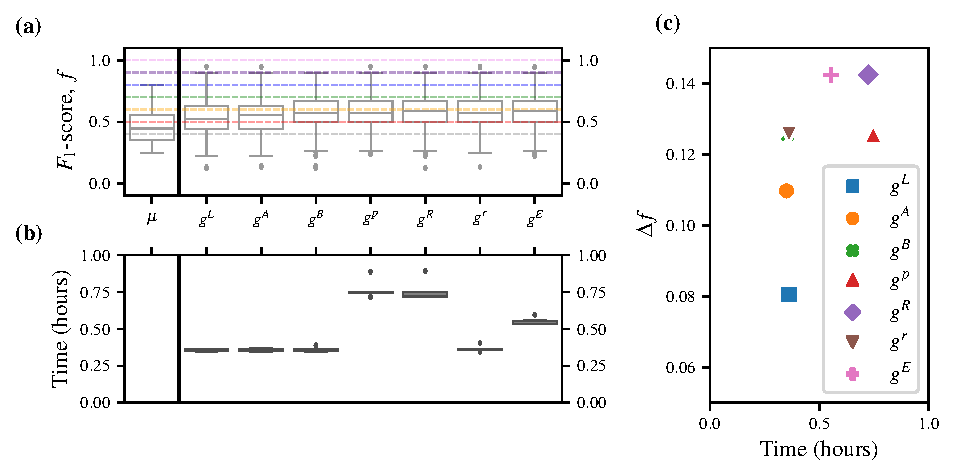
\includegraphics[width=0.95\textwidth]{theoretical_study/figures/objective_fnc_comparison.pdf}
    \caption[Comparison between proposed \glsentrylongpl{of}]{
        Comparison between proposed \glsentryfullpl{of}. 
        Each \gls{of} trains the same initial generation of $N_m=28$ models with resources
        $N_E=500, N_P=2000$, and then design a new set of $N_m$ models through 
        a roulette strategy, such that the only difference between \gls{of}'s output 
        is how they assign selection probability.
        We run each \gls{of} 25 times for the same target system, 
            a $4$--qubit Heisenberg--XYZ model. 
        \textbf{(a)} shows the box--plot of spawned models' \fs, \ $f$, 
            where the median and inter--quartile ranges are indicated by the boxes,
            as well as those of the initial generation $\mu$ centered on $f_{\mu}=0.45$.
            We mark $f=\{0.4, 0.5, ..., 1.0\}$ for ease of interpretation. 
        \textbf{(b)} shows box--plots of the time taken to compute the single generation in each case.
        In \textbf{(c)} we report the difference between the median $f$ among the 
            newly proposed models from $f_{\mu}$, $\Delta f$,
            plotted against the time to achieve the result. 
    }
    \label{fig:obj_fnc_comparison}
\end{figure}

Having proposed a series of possible objective functions, 
    we are now in a position to analyse their appropriateness in the context of \gls{qmla}. 
Recall from \cref{sec:f_score} that we use \fs as the figure of merit against which individual models are measured;
    we can compare \glspl{of} on the basis of the \fs of models they spawn.

\par 

First we can remark on the examples listed in \cref{table:objective_functions}. 
The \glspl{of} which rely on the \gls{tltl}, i.e. $g^L, g^A, g^B, g^r$, 
    are effectively tricked by the log-likelihood, which appears reasonably convincing for 
    poor models, e.g. $\h_a, \h_c$. 
This underlines the risk in buidling $\expset_v$, which can be biased towards weak models, 
    for example resulting in high selection probability for $\h_a$ which has $f=0$, 
    while $\h_d$, with $f=0.4$ is discarded. 
On the other hand, \glspl{of} grounded by the \gls{bf} ($g^p, g^R, g^E$) invariably 
    promote models of higher $\fs$, justifying the role of statistical evidence 
    used for those calculations. 
Overall, however, the insights from this complete example are insufficient to 
    make general claims about the performance of each \gls{of}, 
    so here we examine their outputs systematically. 
\par 

Returning to the task of determining our favoured \gls{of}, 
    we choose some random target $\ho$, and run a single generation of the \gls{ges} with each \gls{of}, 
    allowing us to assess their performance based on the quality of models the \gls{ga} 
    produces under their respective guidance.
We train the same batch of $N_m=28$ random models in each case, and allow each \gls{of} 
    to compute the selection probabilities for those models, 
    and therefore direct the design of the hypothetical next generation of models. 
We plot the distribution of \fs \ that each \gls{of} produces in Fig. \ref{fig:obj_fnc_comparison},
    also accounting for the time taken in each case, i.e. 
    we report the time to train and evaluate the single generation on a 16--core node.
\par

Overall, then, we can see that a strong balance of outcome with resource considerations 
    are achieved by the \gls{bfeer} strategy, \cref{sec:elo},
    so we will use it for the case study presented in this chapter. 
We strongly emphasise, however, that the performance of each objective function
    can vary under alternative conditions, and therefore similar analysis may 
    be warranted for future applications. 
For instance, if $t_{\textrm{max}}$ is known to be small, 
    in smaller model spaces, using $g^r$ results in higher success rates.
We retain \gls{bfeer}, however, for generality and novelty, 
    but it is important to recognise that the results listed do not reflect
    an upper limit of \gls{qmla}'s performance, 
    but rather reflect the constraints of the system under study; 
    each \gls{q} will bring its own unique considerations which can result in 
    significantly stronger or weaker performance under each \gls{of}. 
In particular, we will later use the residual \gls{of}, \cref{sec:residuals}, 
    to study a larger \gls{model space} under assumptions of perfect parameter learning, \cref{chapter:many_qubits}.



\section{Application}
Having introduced all the necessary concepts of \glspl{ga}, 
    mapped them to the \gls{qmla} framework and chosen a suitable 
    \gls{of}, we can finally use the \gls{ges} for model search. 
In summary of this chapter so far, we use the following settings. 
\begin{easylist}[itemize]
    & Models are mapped to a unique bit string (chromosome), where each bit represents whether a given
        model term (gene) is present; chromosomes are of length $N_t$ genes. 
    & A maximum of $N_g$ generations are run, each with $N_m$ unique models. 
    & Candidate models are trained using \gls{qhl}, specifically by using \gls{iqle}\footnotemark \ 
        for parameter estimation. 
    & Models' fitness are determined by their \gls{bfeer}, 
        after having been trained by \gls{qhl} 
        and compared against some set of competing candidate models. 
    & For generating models on $\mu+1$, the models on $\mu$ are first truncated with truncation rate $\tau$; 
        the remaining $\tau N_m$ models are assigned selection probability based on their fitness. 
    & Pairs of models are selected to become parents sequentially using roulette selection. 
        Highly favoured models can parent many offspring models. 
    & Selected parent models are crossed over via a one-point cross-over,
        at crossover location $\kappa \in \left( \frac{N_t}{4}, \frac{3N_t}{4} \right)$, 
        and probabilistically mutated with rate $r_m=0.25$. 
    & The top two elite models from $\mu$ are included on the subsequent generation $\mu+1$.
    & If, after 5 generations, the highest-fitness (elite) model is unchanged, i.e. $\hat{H}_e^{\mu} = \hat{H}_e^{\mu +5}$, 
        we terminate the search and declare that model as the champion, $\hp = \hat{H}_e^{\mu}$. 
    & Otherwise, after $N_g$ generations, the highest-fitness model on the final generation is declared the global champion model, 
        $\hp = \hat{H}_C^{N_g}$.
\end{easylist}
\footnotetext{
    \gls{iqle} assumes complete access to the target system, see \cref{sec:iqle}. 
    This restricts the present analysis to simulateable, rather than physical, use cases, 
    e.g. device calibration. 
}

We will use a four-qubit \gls{model space} under the Heisenberg formalism, \cref{eqn:heisenberg_model_general}, 
    such that any pair of sites $\bkl$ can be coupled by any of the terms $\{\s^x_{\bkl}, \s^y_{\bkl}, \s^z_{\bkl}\}$, 
    so in total there are $N_t = |\termset| = 3 \times {4 \choose 2} = 18$ terms, 
    giving a \gls{model space} of $2^{18} \approx 250,000$ viable models/chromosomes. 
For practical reasons\footnotemark, we set $N_m=60$ and $N_g=16$, although in most cases the 
    elitism clause is triggered so the search terminates long before $N_g$ is reached. 
\footnotetext{
    This is to ensure, with 15 available worker nodes, and accounting for some slowly-learning models, 
    that all $N_m$ models in a generation are trained within $4 t_{\textrm{qhl}}$, 
    where $t_{\textrm{qhl}}$ is the time to train a single model. 
}
The true parameters $\al_0$ are assigned randomly in the range $(0.25, 0.75)$; 
    within \gls{qhl} the prior is set as a multivariate normal distribution $0.5 \pm 0.125$. 
We choose $\ho$ at random to contain half the available terms\footnotemark,
\begin{equation}
    \label{eqn:gen_alg_true_model}
    \ho = \s_{(1, 2)}^{yz}\s_{(1, 3)}^{z}\s_{(1, 4)}^{y}\s_{(2, 3)}^{xy}\s_{(2, 4)}^{x}\s_{(3, 4)}^{xz}.
\end{equation} 
\footnotetext{
    Note we use a compact model representation, e.g. 
    $\hi = \s_{(1, 2)}^{yz}\s_{(1, 3)}^{z} = \s_{(1, 2)}^{y} + \s_{(1, 2)}^{z} + \s_{(1, 3)}^{z}$.
}
\par 
\subsection{Analysis}
We will analyse the \gls{ges} from four perspectives: 
    a single model, a single generation, a single \gls{qmla} \gls{instance}, 
    and the overall performance across many instances, i.e. a \gls{run}.
\par 

\begin{figure}
    \begin{center}
        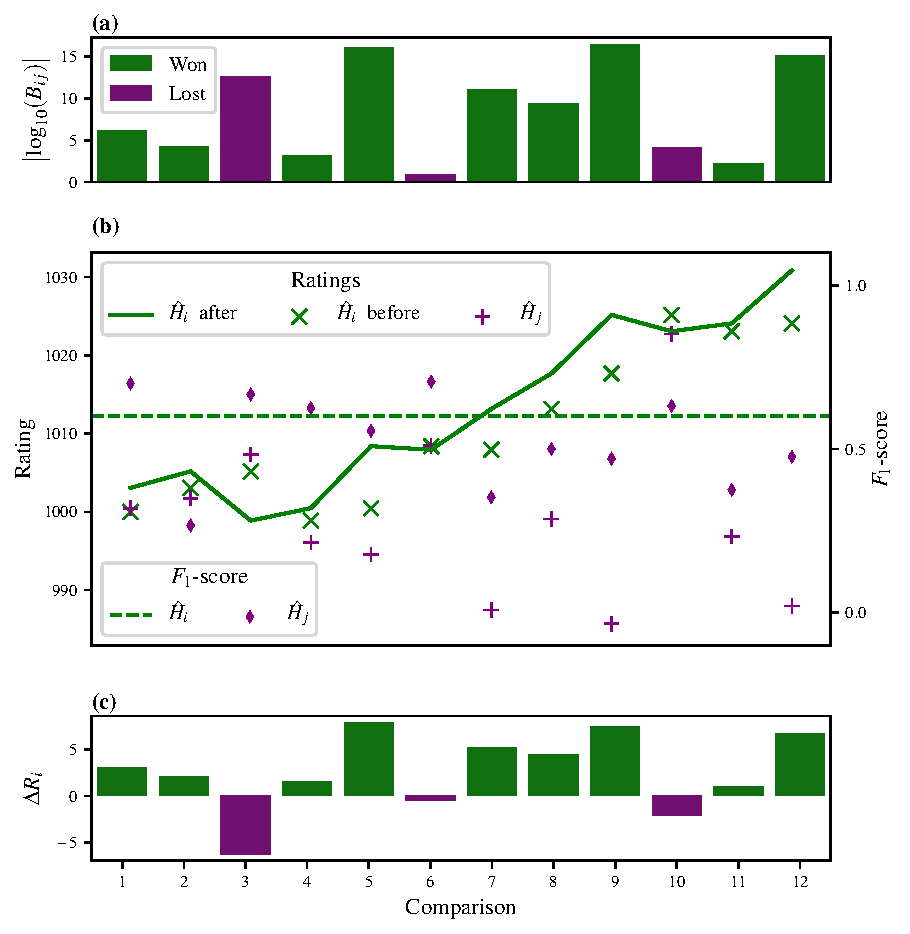
\includegraphics{theoretical_study/figures/single_generation_ratings_progression.pdf}
    \end{center}
    \caption[Single model within a single generation of QMLA genetic algorithm]{
        Progression of \glsentrylong{bfeer}  for a single candidate, $\hi$, within a single generation.
        \textbf{a}, The \glspl{bf} between $\hi$ and some opponents, $\{\hj\}$, 
            from the perspective where $\hi$ \emph{wins} given $\bij > 1 \Rightarrow \log_{10}\bij > 0$, 
            and \emph{loses} otherwise. 
        \textbf{b}, $\hi$'s rating is shown (solid green line) changing according to the \glspl{bf} 
            comparisons with 12 other models from the same generation. 
            Before each comparison, $\hi$'s rating is shown (green cross)
            as well as the rating of its opponent, $\hj$ (purple plus).
            The $F_1$-scores are also shown for $\hi$ (dashed green line) and $\hj$ (purple diamond).
        \textbf{c}, The corresponding change in $\hi$'s rating, $\Delta R_i$. 
        \figtableref
    }
    \label{fig:single_models_elo_ratings}
\end{figure}

Recall that \gls{bfeer} are mediated through random graphs: 
    given $N_m$ models on $\mu$, a given model $\hi$ undergoes some 
    $N_i^{BF} < N_m$ \gls{bf} comparisons. 
In \cref{fig:single_models_elo_ratings} we show the \gls{bf} results 
    and effects on the rating of a random model, $\hi$, where $N_m=60$ and $N_i^{BF}=12$,
    i.e. $\hi$ is directly compared against $20\%$ of contemporary models on $\mu$. 
We see that $\hi$'s rating is effected by whether it wins a given comparison, 
    but also by the strength of evidence provided by the comparison (the \gls{bf}), 
    and the quality of its opposition $\hj$, i.e. the initial rating of $\hj$.
For example, the sixth comparison finds $\hj$ as the superior model, 
    but the evidence is relatively weak and $\hi, \hj$ began with similar ratings, 
    so $R_i$ is not effected drastically. 


\par 
\begin{figure}
    \begin{center}
        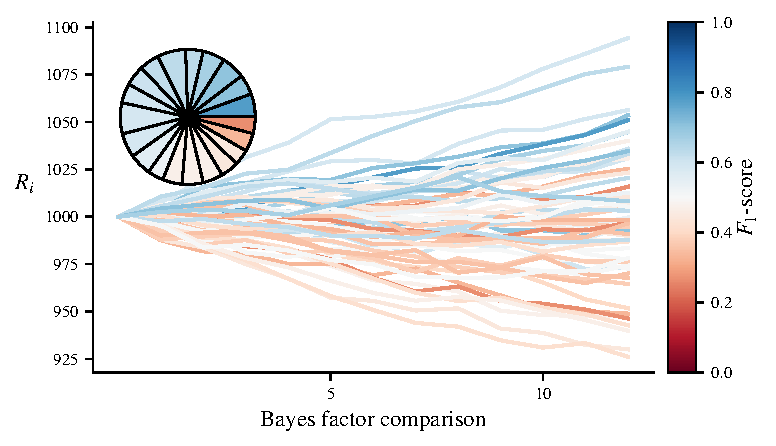
\includegraphics{theoretical_study/figures/single_generation_all_ratings.pdf}
    \end{center}
    \caption[Ratings of all models in a single genetic algorithm generation]{
        Ratings of all $N_m=60$ models in a single \glsentrylong{ga} generation.
        Each line represents a unique model and is coloured by the $\fs$ of that model. 
        \textbf{Inset}, the selection probabilities resulting from the final ratings of this generation. 
        Only $tau=\nicefrac{1}{3}$ of models are assigned selection probability, 
            while the remaining poorer-performing models are discarded. 
        \figtableref
    }
    % TODO replace left of figure with version where elite models are reset to initial rating
    \label{fig:single_generation_all_ratings}
\end{figure}

We extend the single model analysis of \cref{fig:single_models_elo_ratings} to all $N_m$ models 
    in the first generation in \cref{fig:single_generation_all_ratings}.
The general trend is that models of higher $\fs$ have their ratings increased, 
    at the expense of models of lower $\fs$. 
After assessing models thus, the set of models is truncated with rate $\tau=\nicefrac{1}{3}$ to retain only 
    the strongest $20$ candidates,
    which are assigned selection probability, i.e. their chance of being chosen to become a parent during roulette selection, 
    as in \cref{sec:reproduction}.
$N_m$ models are required to populate the next generation:
    the two models with highest $R_i$ -- the \emph{elite} models -- are automatically granted a position;
    the remaining positions are filled through the crossover procedure outlined above.

\par 
\begin{figure}
    \begin{center}
        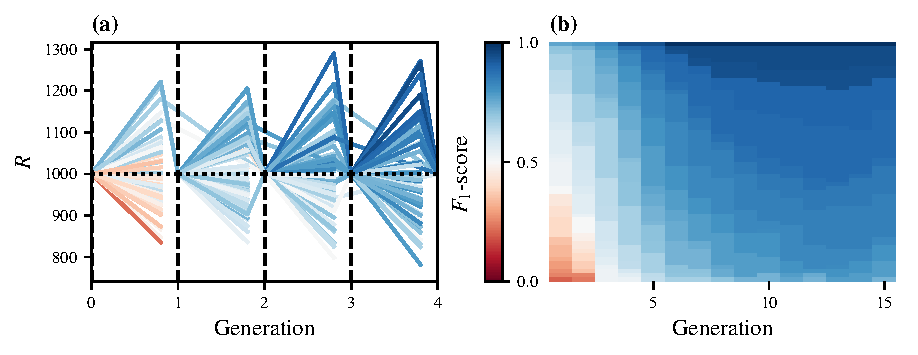
\includegraphics{theoretical_study/figures/gen_alg_instance_combined.pdf}
    \end{center}
    \caption[Instance of QMLA genetic algorithm]{
        A single \gls{instance} of the \gls{qmla} \glsentrylong{}{ga}.
        \textbf{a}, Ratings of all models for the first four generations. 
        Each line in each generation represents a model by its $\fs$. 
        Horizontal dotted lines show the starting rating at that generation. 
        \textbf{b}, Gene pool progression for $N_m=60, N_g=15$. 
        Each tile at each generation represents a model by its $\fs$. 
        \figtableref
    }
    \label{fig:ga_instance}
\end{figure}

We can likewise consider the quality and ratings of models across generations.
In \cref{fig:ga_instance}\textbf{(a)} we see the ratings for models over the first 
    four generations of a \gls{qmla} \gls{instance}:
    the trend suggested by \cref{fig:single_generation_all_ratings} continues,
    where models of higher $\fs$ tend to achieve higher \gls{bfeer}.
The gene pool as a whole tends towards a homogeneous set of high-quality models:
    the final generation consists only of models with $f \geq 0.85$, \cref{fig:ga_instance}\textbf{(b)}. 
Consequently, even in \glspl{instance} where the precise model, $\ho$, is not identified, the \gls{champion model}
    is highly informative, in that it captures many of the same interactions, 
    therefore most-likely providing meaningul insight on the system's physics. 

\par 
\begin{figure}
    \begin{center}
        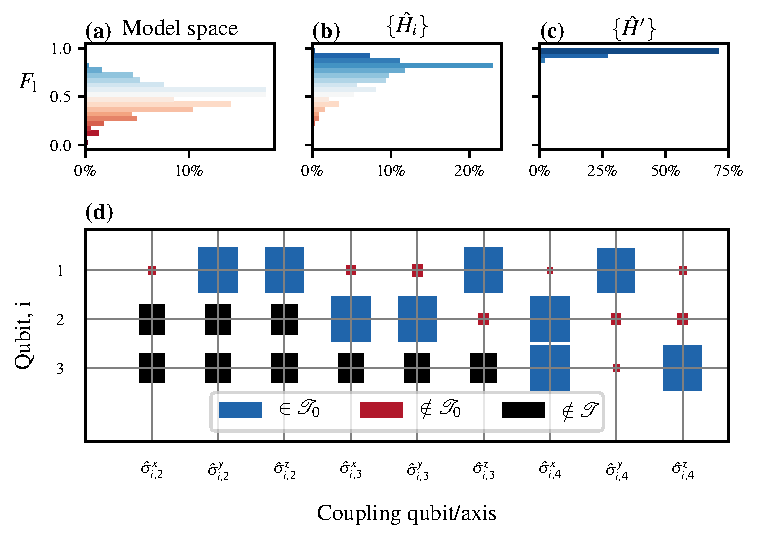
\includegraphics{theoretical_study/figures/gen_alg_run.pdf}
    \end{center}
    \caption[Run of QMLA genetic algorithm]{
        A \gls{run} of the \gls{qmla} \glsentryfull{ga}, consisting of 100 independent \glspl{instance}.
        \textbf{(a)}, The \gls{model space} contains $2^{18}\approx250,000$ candidate models, 
            normally distributed around $f=0.5 \pm 0.14$. 
        \textbf{(b)}, The models explored during the model search of all \glspl{instance} combined, $\{\hat{H}_i\}$.
            \gls{qmla} generates $\sim~43,000$ chromosomes in total across the 100 instances,
                i.e. each \gls{instance} trains $\sim~430$ distinct models;
                Models generated by \gls{qmla} are described overall by a distribution of $f = 0.76 \pm 0.15$, 
        \textbf{(c)}, Champion models from each instance, showing in general \gls{qmla} nominates cahmpion models with
            $f \geq 0.88$ in all instances, 
            and in particular finds the \gls{true model} $\ho$ (with $f=1$) in $72\%$. 
        \textbf{(d)}, Hinton diagram showing the rate at which each term is found in the winning model. 
            The size of the blocks show the frequency with which they are found, while the colour indicates 
            whether that term was (not) in the \gls{true model} in blue (red).
            Terms represetn couplings between two qubits, e.g $\s_{(1, 3)}^{x}$ 
                couples the first and third qubits along the $x$-axis. 
            Available terms involve four qubits with full connectivity, resulting in 18 unique terms 
            (terms with black rectangles are not considered by the \gls{ga}).
        \figtableref
    }
    \label{fig:ga_run}
\end{figure}

Finally, to understand the performance of the \gls{qmla} algorithm overall, 
    we combine 100 independent \glspl{instance} in a \gls{run}, \cref{fig:ga_run}. 
We see that, while the overall \gls{model space} can be characterised by a distribution 
    of models with $\bar{f} = 0.5 \pm 0.14$ (\cref{fig:ga_run}\textbf{(a)}), 
    \gls{qmla} quickly moves to the subspace of high-quality models, 
    i.e. the models explored have median $f = 0.76 \pm 0.15$ (\cref{fig:ga_run}\textbf{(b)}).
This exploration is based on $430 \pm 45$ chromosomes per instance, 
    i.e. \gls{qmla} trains only $0.16\%$ of the $2^{18}$ permitted models. 
Ultimately \gls{qmla} nominates \glspl{champion model} $\{ \hp \}$ with $f \geq 0.88$ in all instances, 
    and precisely identifies $\hp=\ho$ in $72\%$ of instances, \cref{fig:ga_run}\textbf{(c)}. 
Considering the big picture 
    -- where the remit of \gls{qmla} is to identify the interactions \gls{q} undergoes -- 
    we show the rate at which each individual term/gene is included in $\hp$ in 
    \cref{fig:ga_run}\textbf{(d)}. 
Crucially, we see that terms which really are within the true Hamiltonian, $\hat{t} \in \termset_0$, 
    are found at a higher rate than those without, $\hat{t} \notin \termset_0$. 
This level of analysis can be used to post-validate the outcome of \gls{qmla}, 
    i.e. rather than relying on $\hp$ from a single instance, 
    trusting the terms' individual frequencies as evidence that they are of importance when describing 
    the system of interest. 
\par 

\subsection{Device calibration}
The use-case presented in this chapter is restrictive,
    so cannot be considered as a solution to characterising any black box quantum system.
Firstly, the set of conceivable terms must be prescribed in advance to facilitate a chromosome mapping;
    this either limits the range of insight \gls{qmla} can achieve to interactions envisaged by the user,
    or requires a vast set of permissible terms, leading to substantially longer model search phases than shown here. 
Secondly, models were trained using \gls{iqle} in order to learn effectively with relatively few resources. 
\gls{iqle} is only available to train models where we can reliably reverse the evolution of the target system 
    (see \cref{sec:iqle}), and as such it is only useful when we have complete control over \gls{q}, 
    for example where \gls{q} is some quantum simulator. 
\par 
The adaptive \gls{ges} presented in this chapter may therefore prove a useful 
    application of \gls{qmla} in the domain of device calibration,
    in particular to characterise some untrusted quantum simulator.
That is, by using the simulator to implement some target $\ho$, 
    \gls{qmla} can identify which operator is \emph{actually} implemented.
For instance, implementation of a four--qubit model
    relies on high-fidelity two-qubit gates between arbitrary qubit pairs.
\gls{qmla} can effectively reconstruct which operations were and were not faithfully computed,
    i.e. determine in which operations the device failed to perform the intended calculations,
    allowing for the calibration of said device. 
The extension of \gls{qmla} to the characterisation of real quantum devices is one of the main 
    recommendations for future research in the scope of the \gls{qmla} framework beyond this thesis.  

\part{Experimental Studies}\label{part:experimental_study}
    \chapter{Nitrogen Vacancy centre}\label{chapter:nv}
        
It is of primary interest to apply the \gls{qmla} algorithm to real-life, experimental systems. 
In this chapter we devise an \gls{es} to operate in conjunction with experimental data 
    in order to characterise an electron spin in a \gls{nvc} in diamond.
In particular, we model, through \gls{hamiltonian} terms, interactions between the spin and 
    the spin bath in which it resides,
    so that \gls{qmla} is finding an effective model for the open system dynamics.
\par

Here we will first introduce a basic picture of \glspl{nvc}, 
    using basic but nonstandard nomenclature for simplicity;
    for thorough descriptions of the underlying physics, readers are referred to \cite{doherty2013nitrogen}.
We next discuss the target system with respect to its modelling, 
    determining the suitable terms which \emph{might} represent the \gls{nvc}'s interactions, 
    to inform the starting point for \gls{qmla}.
Finally we describe the implementation of an \gls{es} for the examination of the \gls{nvc},
    and the results of the \gls{qmla} procedure. 

\section{Nitrogen-vacancy centre}
\label{sec:nv_centres}

Nitrogen vacancies are point defects in diamond, 
    occuring intrinsically (naturally) \cite{davies1976optical} or extrinsically (synthetically) \cite{meijer2005generation, edmonds2012production}.
A substitutional \gls{nitrogen} isotope is embedded in a lattice of carbon atoms in diamond, 
    adjacent to a lattice vacancy, 
    such that it is surrounded by three \glspl{carbon} (either $^{12}C$ or $^{13}C$) \cite{lenef1996electronic}. 
Of the \gls{nitrogen} atom's five valence electrons, three bond with nearby \glspl{carbon};
    the remaining two unbonded electrons couple with the lattice vacancy, 
    forming a triplet state, considered as the \gls{nvc}. 
We can experimentally drive the outer electron, moving the \gls{nvc} between energy levels characterised by the triplet. 
In this section we describe how we can exploit those energy levels in order to define a mechanism by which to 
    prepare and implement gates on the controlled system, a readout procedure and a computational basis.

\par 

A \emph{manifold} is a set of states with marginal differences, such as a single differing quanutm number.
For example, states near the absolute ground state might differ only in their magnetic spin quantum number:
    together they can be characterised as the \emph{ground state manifold}. 
We consider two principal manifolds of the system:
    the ground state and excited manifolds, each consisting of 
    three states, corresponding to the allowed values for magnetic spin $m_s$, see \cref{fig:nv_centre_energy_levels}a. 
For brevity, we denote states with reference to their magnetic spin and manifold, 
    e.g. the state in the ground state manifold with $m_s=0$ is denoted $\ket{m_s=0}_g$. 
In the absence of a magnetic field, the states corresponding to $\ket{m_s=\pm1}$ are degenerate, 
    but in the presence of a magnetic field, $B$, they have distinct energy levels, 
    referred to as the Zeeman effect, \cref{fig:nv_centre_energy_levels}b. 
\par 

For the purposes of computation, 
    we choose the ground state and one of the excited states as the two levels of a qubit. 
We designate the states $\ket{m_s=0}_g$ and $\ket{m_s=-1}_g$ as the computational basis states $\ket{0}, \ket{1}$ respectively, 
    such that we have defined a qubit and computational basis, \cref{fig:nv_centre_energy_levels}d.
We also require a reliable mechanism through which we can be confident that our qubit is in a definite state, 
    to serve as the starting point of computation: 
    usually qubits are initialised to $\ket{0}$, 
    so here we aim to prepare the \gls{nvc} in $\ket{m_s=0}_g$.
By shining a laser of \SI{532}{\nano\metre} (green) on the \gls{nvc}, irrespective of which state within the ground state manifold the spin starts, 
    it is excited in to the excited manifold, from which it decays back to the ground state manifold.
The process of this decay can be exploited for the preparation of the \gls{nvc} in $\ket{m_s=0}_g$ 
    and therefore enable initialisation for computation.
That is, when the \gls{nvc} is excited to the $\ket{m_s=0}_e$ level, the dominant decay process is spin-preserving, 
    so after decay it ends in $\ket{m_s=0}_g$. 
On the other hand, if the \gls{nvc} had been excited instead to $\ket{m_s=\pm1}_e$,
    the dominant decay process is through a meta-stable/shelving state, 
    which does not preserve spin, so in this case it also ultimately decays to the $\ket{m_s=0}_g$, \cref{fig:nv_centre_energy_levels}\textbf{(c)}.
Therefore, irrespective of the initial state, 
    by shining the green laser on the \gls{nvc} and exciting it into any of the states in the excited manifold, 
    after decay it is most likely that it has been prepared in $\ket{m_s=0}_g = \ket{0}$, 
    providing a starting point from which to perform computation.
\par 

The difference in energy between our defined computational basis states $\ket{0}$ and $\ket{1}$ is 
    $\sim 2.87 \ghz$, i.e. it is addressible by \gls{mw} radiation.
Via antenna, we can deliver a \gls{mw} pulse upon the \gls{nvc}, driving the \gls{nvc} between the two levels
    providing an implementation of an \ttt{X}-gate. 
Likewise, having initialised the state to $\ket{0}$, we can perform a $\nicefrac{\pi}{2}$ rotation 
    about the logical $z$-axis, by running the \gls{mw} laser for half the time, 
    resulting in the state $\ket{+}$. 
We can similarly devise \gls{mw} radiation to achieve quantum gates and operations on our \gls{nvc} qubit.
We depict these cycles in \cref{fig:nv_centre_energy_levels}c. 
\par

\begin{figure}[t]
    \begin{center}
        \includegraphics[width=0.95\linewidth]{experimental_study/figures/nv_centre_cartoon.pdf}
    \end{center}
    \caption[\Glsentrylong{nvc} energy levels]{
        Simplified depiction of energy levels of the \glsxtrlong{nvc}, corresponding to its triplet state. 
        \textbf{a}, With no external magnetic field, the system has excited and ground-state manifolds, 
            each of which consist of two energy levels depending on the magnetic spin, $m_s$.
        \textbf{b}, In the presence of a magnetic field (purple, $B$), the magnetic spins have distinct energy levels, 
            i.e. Zeeman splitting giving distinct $m_s$. 
        States are denoted by their magnetic spin, $m_s$ and subscripted by their manifold ($e$ for excited and $g$ for ground-state). 
        \textbf{c},  Application of a \SI{532}{\nano\metre} laser (green arrow) excites the \glsxtrlong{nvc} from any of the states in the 
            ground state manifold into the excited manifold. 
        The dominant decay mechanism for the excited states are shown: 
            (i) $\ket{m_s=0}_e \rightarrow \ket{m_s=0}_g$ (\glsxtrlong{pl}, red) through the emission of a photon at \SI{637}{\nano\metre});
            (ii) $\ket{m_s=\pm 1}_e \rightarrow \ket{m_s=0}_g$ (dotted grey lines) via the shelving manifold which allows for non-spin-preserving transition, 
            emitting a photon in the infrared (not shown).
        \textbf{d}, Computational basis states $\ket{0}$ and $\ket{1}$ are assigned to the two lowest energy states.
            The difference in energy between these states is such that a microwave (MW, blue) 
                can drive transition from $\ket{0} \leftrightarrow \ket{1}$.
            MW pulses can also be used to achieve other states apart from the basis states,
                allowing for the implementation of quantum logic gates. 
    }
    \label{fig:nv_centre_energy_levels}
\end{figure}


We can further exploit the decay mechanism to compose a readout procedure, 
    to infer the population of $\{\ket{0}, \ket{1}\}$ at a given instant, 
    for example following the application of a series of gates (a circuit) to the system. 
We know that the excitation due to the green laser is spin-preserving, 
    i.e. when the \gls{nvc} has been excited to $\ket{m_s=0}_e$, 
    it had originated in $\ket{m_s=0}_g$.
We also know that the decay $\ket{m_s=0}_e \rightarrow \ket{m_s=0}_g$ is spin preserving, with the emission of 
    a red photon: by simply counting the number of excess\footnotemark \ photons emitted, 
    we quantify the population of $\ket{0}$ at the time of query. 
On the contrary, when the $\ket{m_s=-1}_g$ is excited, 
    spin is also preserved, so it goes to $\ket{m_s=-1}_e$, 
    but $\ket{m_s=-1}_e$ decays through the shelving state as outlined earlier, 
    \emph{without} the emission of a red photon (the decay emits out infrared radiation instead). 
We can hence infer the population of $\ket{m_s=-1}_g$ at the time of query by the fraction of incidents which don't 
    emit a photon \cite{knauer2016photonic}.
That is, say we first calibrate the system by retaining the green laser for some time: 
    after a few $\mu s$, a steady state is achieved where the majority of the time, the triplet is in the computional state $\ket{0} = \ket{m_s=0}_g$. 
Then, excitation from the same laser results in the excitation to $\ket{m_s=0}_e$, 
    which decays back to $\ket{m_s=0}_g$ and emits a photon in the process; 
    by counting the red photons emitted in a certain time window -- equivalently, measuring the \gls{pl} signal -- 
    we benchmark the population of $\ket{0}$ when nothing else has happened as $p_0$. 
Now, when we apply gates (i.e. \gls{mw} pulses) to the \gls{nvc}, 
    we can similarly read out the population of $\ket{0}$ as $p_0^{\prime}$,
    and infer that the likelihood that the \gls{nvc} is found in the initial state $\ket{0}$ is $\nicefrac{p_o^{\prime}}{p_0}$. 
We can use this quantity as the  \gls{likelihood} within \gls{qle}, allowing us to learn from the \gls{nvc},
    as we will discuss in the next sections. 

\footnotetext{
    A large number of photons are emitted by the \gls{nvc} when it is excited by a \SI{532}{\nano\metre} laser,
    which can be profiled by its emission spectrum. 
    At the \emph{zero phonon line} (\SI{637}{\nano\meter}),
    a relatively large number of photons are emitted, compared with nearby wavelengths.
    This is where decay from the excited to ground state occurs without interacting with proximal phonons, 
        as is the case during the spin-preserving decay $\ket{m_s=0}_e \rightarrow \ket{m_s=0}_g$.
    The excess photons are taken as indication that the electron had been in the state $\ket{m_s=0}_e$ immediately prior to emission.
}
\par 

In summary then, by assigning basis states $\ket{0}, \ket{1}$ to energy levels of the ground state manifold, 
    we are able to ensure the preparation of the \gls{nvc} in $\ket{0}$ by first shining a green laser on the \gls{nvc}. 
We can then apply \gls{mw} radiation to achieve quantum logical gates on the system, 
    and read out the final state of the system, again by shining a green laser
    and observing the \gls{pl} (i.e. the emitted photons), and inferring the population level of each basis state. 
We represent these concepts in a simplified format in \cref{fig:nv_centre_energy_levels}. 

\subsection{Experimental procedure}
\begin{figure}
    \begin{center}
        \subfloat[]{
            \includegraphics[width=0.25\textwidth]{experimental_study/figures/hahn_bloch_spheres/bloch_0.pdf}
        }
        \qquad
        \subfloat[]{
            \includegraphics[width=0.25\textwidth]{experimental_study/figures/hahn_bloch_spheres/bloch_1.pdf}
        }
        \qquad
        \subfloat[]{
            \includegraphics[width=0.25\textwidth]{experimental_study/figures/hahn_bloch_spheres/bloch_2.pdf}
        }
        \\
        \qquad
        \subfloat[]{
            \includegraphics[width=0.25\textwidth]{experimental_study/figures/hahn_bloch_spheres/bloch_3.pdf}
        }
        \qquad
        \subfloat[]{
            \includegraphics[width=0.25\textwidth]{experimental_study/figures/hahn_bloch_spheres/bloch_4.pdf}
        }
        \qquad
        \subfloat[]{
            \includegraphics[width=0.25\textwidth]{experimental_study/figures/hahn_bloch_spheres/bloch_5.pdf}
        }
    \end{center}
    \caption[States of spin qubit at each stage of Hahn echo sequence shown on the Bloch sphere]{
        States of spin qubit at each stage of Hahn echo sequence shown on the Bloch sphere.
        \textbf{a,} The state of the \gls{nvc} spin is initialised by a green laser into state $\ket{\psi_0} = \ket{0}$. 
        \textbf{b,} We apply a $\nicefrac{\pi}{2}$ rotation about the $y$-axis (i.e. a \glsxtrfull+{mw} pulse, implemented as $e^{-i \frac{\pi}{4} \s_y}$), 
            yielding the state $\ket{\psi_1} = \ket{+}$. 
        \textbf{c,} The system is allowed to evolve according to its own $\ho$ for $t$, $\ket{\psi_2} = e^{-i\ho t}\ket{+}$.
        \textbf{d,} We apply a second \gls{mw} pulse, this time for a $\pi$-rotation about the $y$-axis, 
        $\ket{\psi_3} = e^{-i\frac{\pi}{2} \s_y}e^{-i\ho t}\ket{+}$.
        \textbf{e,} Again the system evolves according to interactions with the environment, this time for $t^{\prime}$.
        \textbf{f,} We apply a final $\nicefrac{\pi}{2}$ \gls{mw} pulse to rotate about the $y$-axis again, 
            projecting it upon $\ket{0}$.
        Here $\ket{\psi_5}$ is roughly half way between $\ket{0}$ and $\ket{+}$, 
        i.e. along the $z$-axis. 
        The spin is read out from $\ket{\psi_5}$ via the \gls{nvc}'s \glsxtrlong{pl}. 
        Here $\ho = 0.25 \ \s_y$ was evolved for $t=0.5$ (arbitrary units), 
        and the final state overlap with the initial state, 
        i.e. the \gls{likelihood} of measuring the spin in $\ket{0}$ is $\Pr(0 | \ho, t) = 0.865$. 
    }
    \label{fig:hahn_bloch_spheres}
\end{figure}

As our primary objective, we aim to model the decoherence and precession of the \gls{nvc} (described in \cref{sec:target_system}), 
    and therefore must implement an experimental strategy which highlights 
    the decoherence effects dominating the spin. 
The \emph{Hahn echo sequence} is a series of operations which decouple a spin from the  
    slowly varying components of its environment, i.e. the nuclear bath
    \cite{blok2014manipulating, childress2006coherent, rowan1965electron, charnock2001combined, gentile2020Operating}.
For short evolution times, i.e. in the first decay of the \gls{nvc}, the spin is influenced mostly by \emph{fast} decoherence processes,
    providing a platform to study the contributions of dominant decoherence effects in isolation. 


\par 
During the Hahn echo sequence, the \gls{nvc} spin undergoes a series of evolutions -- 
    either according to application of quantum logic gates
    or the natural evolution of the system interacting with its environment.
Intuitively, the stages are as follows: 
\begin{enumerate}[label=(\alph*)]

    \item Prepare spin in $\ket{0}$.
    \item Apply a $\nicefrac{\pi}{2}$ \gls{mw} pulse. 
    A $\pi$-pulse is a \gls{mw} pulse of sufficient duration to flip the spin completely ($\ket{0} \leftrightarrow \ket{1}$), 
    so a $\nicefrac{\pi}{2}$-pulse generates a superposition, i.e. $\nicefrac{\pi}{2}: \ket{0} \rightarrow \ket{+}$.
    \item The superposition precesses freely for $t$. During this time, the $\ket{1}$-component of the superposition picks
        up a phase proportional to $t$, such that the spin is now in the state $\frac{1}{\sqrt{2}}\left( \ket{0} + e^{-i \delta t}\ket{1}\right)$. 
    \item A \gls{mw} $\pi$-pulse is applied, which inverts the basis states, yielding the state $\frac{1}{\sqrt{2}}\left( \ket{1} + e^{-i \delta t}\ket{0}\right)$.
    \item The spin is again allowed precess freely, here for a duration $t^{\prime}$. 
        Again the $\ket{1}$-copmonent gains a phase $e^{-i \delta t^{\prime}}$, 
        i.e. the spin is in the state $\frac{1}{\sqrt{2}}\left( e^{-i \delta t}\ket{0} + e^{-i \delta t^{\prime}}\ket{1} \right)$.
    \item A final $\nicefrac{\pi}{2}$ pulse is applied, giving 
        $\frac{1}{\sqrt{2}}\left( e^{-i \delta t}\ket{+} + e^{-i \delta t^{\prime}}\ket{-} \right)$.
        Expanding $\ket{+}, \ket{-}$ and factoring $e^{-i \delta t}$, we get the final state
        \begin{equation}
            \ket{\psi_H(t, t^{\prime})} = \frac{e^{-i \delta t}}{2} \left\{ (1 + e^{-i \delta(t^{\prime} - t)})\ket{0} + (1 - e^{-i \delta(t^{\prime} - t)})\ket{1}  \right\}.    
        \end{equation}
\end{enumerate}

If the second free evolution is run for $t^{\prime} = t$, we retrieve
\begin{equation}
    \ket{\psi_H(t, t^{\prime}=t)} = \frac{e^{-i \delta t}}{2} \left\{ (1 +1)\ket{0} + (1 - 1)\ket{1}  \right\} = \ket{0},    
\end{equation}
    i.e. the phase accumulated is effectively removed. 
This is therefore an excellent scheme when seeking to isolate the spin from its environment, 
    e.g. when the spin is intended to act as a qubit. 
In practice it is impossible to decouple the environment entirely, 
    since distant nuclei still interact with the spin, % TODO why are these not cancelled out by the same phase reversal?
    causing decoherence on a relatively long time scale\footnotemark.
These are what we refer to as \emph{slow} interactions: 
    this decoupling scheme can therefore be viewed as corresponding to a model 
    where the Hamiltonian consists solely of slow terms, 
    enabling us to study the spin's interactions with its environment beyond 
    the nearest \gls{carbon} atom.
We will explore this possibility in \cref{chapter:many_qubits}.
\footnotetext{
    The timescales on which these interactions decohere the spin are orders of magnitude higher
    then available through alternative decoupling schemes,
    e.g. $T_2 = \SI{242 }{\micro\second}$ in \cite{childress2006coherent}.
}
\par 

On the other hand, when $t^{\prime} \neq t$, the spin is instead found in the state
\begin{equation}
    \label{eqn:hahn_unequal_times}
    \ket{\psi_H(t, t^{\prime}\neq t)} = \frac{e^{-i \delta t}}{2} \left\{ (1 + e^{-i \delta(t^{\prime} - t)})\ket{0} + (1 - e^{-i \delta(t^{\prime} - t)})\ket{1}  \right\}.
\end{equation}

\cref{eqn:hahn_unequal_times} has the precise form (up to the phase factor $e^{-i \delta t}$)
    of a spin having undergone a \emph{Ramsey sequence}, 
    i.e. a $\nicefrac{\pi}{2}$ pulse, followed by free evolution for $t$, and a final $\nicefrac{\pi}{2}$ pulse.
That is, for $t^{\prime}\neq t$, the Hahn echo sequence behaves like 
    a Ramsey sequence with a delay $(t^{\prime} - t)$ \cite{childress2007coherent}. 
$\ket{\psi_H(t, t^{\prime}\neq t)}$ therefore does \emph{not} decouple the spin from its dominant dephasing contributions, 
    but rather it reverses the dephasing due to \emph{slowly varying} components of the environment. 
As such, this provides a platform for examining only the \emph{fast} effects on the spin, 
    i.e. the dominant Markovian decoherence processes, which are expected to be dominated by 
    coupling with the nearest \gls{carbon} atom of strength $\mathcal{O}(\SI{}{\mega\hertz})$. 
\par 

In \cref{chapter:many_qubits}, we consider the system more broadly, and endeavour to 
    characterise its coupling with several nuclei, located farther from the spin than the nearest \gls{carbon},
    i.e. the slower-varying contributions to the spin's dynamics, 
    which an be examined via the former scheme with $t^{\prime} = t$. 
For the remainder of this chapter, however, we will exploit the latter scheme, \cref{eqn:hahn_unequal_times}, 
    in order to model the decoherence of the spin via its relationship with a single \gls{carbon} atom. 
\par 

To relate the experimental procedure to the parameter learning technique described in \cref{chapter:qhl}
    which fulfils the training stage of \gls{qmla}, consider the overal Hahn echo sequence.
We depict the stages of the experiment more generally in \cref{fig:hahn_bloch_spheres}, 
    starting from the initialised computational state, $\ket{\psi_0} = \ket{0}$,
    through to its final state which is read out through \gls{pl},
    both of which as described in \cref{sec:nv_centres}.
In particular, the final state, $\ket{\psi}_5$, is effectively read out by projection onto $\ket{0}$;
    we can interpret the normalised \gls{pl} after evolution time $t$ as the  \gls{likelihood} 
    that the \gls{nvc} is found in $\ket{0}$ after evolution of its \emph{true}\footnotemark \ Hamiltonian, $\ho$ for $t$. 
\footnotetext{
    Note: we refer to the target $\ho$ as the system's \emph{true} Hamiltonian. 
    This is a matter of convention: 
        here $\ho$ is not the Hamiltonian of the complete \gls{nvc} system/environment, 
        but captures only the precession and fast decoherence processes, 
        i.e. $\ho$ is simply the name assigned to the Hamiltonian which models the interactions we aim to uncover. 
}
That is, we assign this projection as the quantity $\Pr(0 | \ho, t)$ (the  \gls{likelihood}), 
    and it can be used within \gls{likelihood} estimation in order to refine a candidate model $\hj$, 
    effectively\footnotemark \ by changing the structure of 
    $\hj$ until $\Pr(0 | \ho, t) \approx \Pr(0 | \hj, t) \ \forall t$. 

\footnotetext{
    Of course this is a gross simplification of \gls{qhl} which is described fully in \cref{chapter:qhl}
}
\par 

By varying the evolution time, $t$, used within the Hahn echo sequence, we can map the \gls{likelihood} against time, 
    which we can view as capturing the \emph{dynamics} of the \gls{nvc} spin, \cref{fig:nv_raw_data}.
We vary the evolution time up to $t \sim 4 \mu s$ in intervals of $\Delta t = 50 \SI{}{\nano\second}$, 
    so we have 425 data points. 
Note the data for the studied \gls{nvc} is taken once and analysed offline, 
    i.e. \gls{qmla} does not have complete authority to design \glspl{experiment} 
    to run on the \gls{nvc}, although it can aim to choose the most informative $t$ 
    available in the predefined set; we will discuss the consequences of this restriction 
    in \cref{sec:nv_constraints}. 

\begin{figure}[t]
    \begin{center}
        \includegraphics{experimental_study/figures/raw_data.pdf}
    \end{center}
    \caption[Raw data for nitrogen-vacancy centre's dynamics]{
        Raw data for the \glsxtrlong{nvc}'s dynamics.
        The $y$-axis shows the normalised \glsxtrlong{pl} of the \gls{nvc}, 
        equivalently the \gls{likelihood} $\Pr(0 | \ho, t)$. 
    }
    \label{fig:nv_raw_data}
\end{figure}

\newpage
\section{Target system}\label{sec:target_system}
We take the axis of the \gls{nvc}, i.e. the axis connecting the \gls{nitrogen} with the 
    lattice vacancy, as the $z$-axis.
While the \gls{nvc} is subject to myriad interactions which result in decoherence,
    we choose to focus on its dominant interactions with proximal environmental nuclei. 
These interactions are characterised by hyperfine terms \cite{smeltzer201113c}.
The complete \gls{hamiltonian} for such systems, where the set of nuclear sites is $\{\chi\}$,
    is expected to be given by 

\begin{equation}
    \label{eqn:nv_ham_full}
    \hat{H}_{\mathrm{\textrm{full}}} 
    = 
    \Delta_{\textrm{gs}} \hat{S}_z^2 
    + \mu_B g \mathbf{B} \cdot \mathbf{S} 
    + \mathbf{S} \cdot \sum_{\chi} \left( \mathbf{A}_{\chi} \cdot \hat{I}_{\chi} \right) 
    + P \hat{I}_z^2 
    + \mu_n g \mathbf{B} \cdot \sum_{ \chi} \hat{I}_{\chi}.
\end{equation}

Our overarching intention is to design an approximate model $\hp$, 
    i.e. a subset of the terms in $\hat{H}_{\textrm{full}}$ which can explain the observed dynamics 
    and decoherence of the \gls{nvc}. 
It is therefore prudent only to retain terms which \emph{may} contribute to the spin's decoherence and precession. 
First, we will describe each term in \cref{eqn:nv_ham_full}, 
    as well as approximations which enable us to drastically reduce the space of terms to consider for inclusion in $\hp$. 

\begin{description}
    \item[Isolated-spin terms] \
    
    Describe the spin independent of the environmental nuclei
    \begin{easylist}[itemize]
    && $\Delta_{\textrm{gs}} \hat{S}_z^2$: 
        the \emph{zero-field} splitting, or ground state splitting between the computational basis states.
        $\Delta_{\textrm{gs}} \sim \ghz$ is a constant offset which does not contribute to the decoherence, 
        so it is excluded from our study.

    && $\mu_B g \mathbf{B} \cdot \mathbf{S}$: 
        the spin's precession about the magnetic field, 
        $\mathbf{B} = \left(B_x \  B_y \  B_z\right)$, 
        via the total spin operator\footnotemark \ $\mathbf{S} = \left(\hat{S}_x \ \hat{S}_y \ \hat{S}_z \right)$, 
        where $\mu_B$ is the Bohr magneton and $g$ is the electron $g$-factor 
        ($\approx 2$, simplified from the $g$-factor tensor).
        Misalignment of the magnetic field is a decoherence effect, 
        so one core aim of \gls{qmla} in this setting is to identify whether such terms dominate.
    \end{easylist}
    
    \item[Hyperfine terms] \ 
    \begin{easylist}
    && $\hat{S} \cdot \sum_{\chi} \left( \mathbf{A}_{\chi} \cdot \hat{I}_{\chi} \right)$:
        The \gls{nvc} total spin operator $\mathbf{S}$ couples the spin with each site, $\chi$.
        At each site there is a nucleus which has total spin operator 
        $\mathbf{I}_{\chi} = \left(\hat{I}_x \ \hat{I}_y \ \hat{I}_z \right)_{\chi}$. 
        $\mathbf{A}$ is the hyperfine tensor, containing the hyperfine parameters of interest. 
        The coupling between the \gls{nvc} and these nuceli is one of the primary decoherence mechanisms, 
        so is essential to any model aiming to capture those dynamics. 
    \end{easylist}

    \item[Bath-only terms] \
    
    Describe the other nuceli independent of the spin
    \begin{easylist}        
    && $P \hat{I}_z^2 $: the quadrupole splitting, which provides another constant shift, 
        and is therefore not of interest when modelling the spin's decoherence, and can be neglected.
    && $\mu_n g \mathbf{B} \cdot \sum_{ \chi} \hat{I}_{\chi}$:
        nuclear precession terms. 
        $\mu_n$ is the nuclear magneton and $g$ is the nuclear $g$-factor (again from the $g$-factor tensor).
        These terms represent the nuclei independent of the spin -- 
        these terms lead to decoherence at much higher times than we have access to, since the Hahn echo sequence decouples the spin from the bath. 
        For the short-time model targeted here, then, these terms can be excluded. 
    \end{easylist}

\end{description}

\footnotetext{
    We invoke an inexact representation of high dimensional tensors here for ease of interpretation. 
    For instance, the total nuclear spin operator exists in arbitrary dimension 
    (depending on the number of sites modelled), 
    but we present it simply as $\mathbf{I} = \left( \hat{I}_x \ \hat{I}_y  \ \hat{I}_z \right)$ at each site 
    to convey that we can separate the terms in the construction of models. 
}

Given that we are modelling the spin's decoherence, 
    we are interested only in the spin and its interactions with the environment, 
    so we can immediately drop the bath-only terms, 
    by assuming the bath is static apart from its interactions with the \gls{nvc}. 
This is a usual assumption in the treatment of open system dynamics, 
    to allow for focus on the dominant interactions in the processes of interest \cite{breuer2002theory}. 
Additionally, since the zero field splitting contributes a constant shift in energy, 
    we can safely omit it by moving to the rotating frame. 
We are then left only with the second and third terms of \cref{eqn:nv_ham_full}, 
    from which to define the space of terms in which \gls{qmla} will search:

\begin{subequations}
    \begin{equation}
        \label{eqn:nv_spin_terms}
        \mu_B g \mathbf{B} \cdot \mathbf{S};
    \end{equation}
    \begin{equation}
        \label{eqn:nv_hyperfine_terms}
        \mathbf{S} \cdot \sum_{\chi} \left( \mathbf{A}_{\chi} \cdot \mathbf{\hat{I}}_{\chi} \right).
    \end{equation}
\end{subequations}

\subsection{Mapping to model terms}
Next we will focus on mapping the remaining terms to operators to compose the set of terms 
    $\termset$ to use in our \gls{es}. 
In our modelling, the \gls{nvc} spin is represented by the first logical qubit, 
    with a further $|\{\chi\}|$ qubits, each representing a unique nuclear site, 
    as discussed later in this section. 
As standard, we take the axis\footnotemark \ of the \gls{nvc} as parallel to the qubit's $z$-axis. 

\footnotetext{The quantisation axis, i.e. the axis along the \gls{nitrogen} and lattice vacancy.}
\par 

The first terms included, \cref{eqn:nv_spin_terms}, come from the spin's precession about the magnetic field. 
It is usually assumed that the external, applied magnetic field is well-aligned with the spin qubit's $z$-axis:
    if the field is misaligned, it leads to decoherence effects. 
Determining the alignment is treated as a core role of \gls{qmla}, 
    i.e. we will endeavour to establish whether the $x$-, $y$-axis components of the magnetic field 
    are important for describing the spin's decoherence. 
Then, we have
\begin{equation}
    \label{eqn:spin_tensor_terms}
    \mu_B g \mathbf{B} \cdot \mathbf{S} 
    = \mu_B g \irow{B_x & B_y & B_z} \cdot \irow{\hat{S}_x & \hat{S}_y & \hat{S}_z}
    \rightarrow \alpha_x \hat{S}_x + \alpha_y \hat{S}_y + \alpha_z \hat{S}_z,
\end{equation}
with $\alpha_i = \mu_B g B_i$. 
The spin's rotation terms to be included in \gls{qmla}'s deliberations are therefore 
\begin{equation}
    \label{eqn:exp_spin_terms}
    \termset_{s} = \{ \hat{S}_x, \  \ \hat{S}_y, \ \ \hat{S}_z\}.
\end{equation}
\par 

Next, we consider the hyperfine coupling term. 
In general we sum over the nuclear sites $\{ \chi \}$, 
    since  the \gls{nvc} spin will interact with every nucleus within a certain range.
We show in \cite{gentile2020learning} that a realistic system requires modelling a 
    finite-size bath of $|\{\chi\}|\sim 15$ 
    nuclei to capture the dynamics of interest, 
    which is infeasible for complete characterisation via classical simulation, 
    where we are limited to $\sim 11$ qubit calculations\footnotemark. 
Instead, by focusing only on the \emph{short-time} dynamics of the \gls{nvc}, 
    we can isolate the effects of dominant interactions, 
    most notably with a single nearby \gls{carbon}. 
Indeed, by assigning a first qubit as representing the \gls{nvc} spin, 
    we can map the entire environment onto a generic second \emph{environmental qubit}, 
    representing the amalgamation of said interactions, 
    though we can think of the two-qubit system as the \gls{nvc} coupled with a single \gls{nitrogen} \cite{smeltzer201113c}. 

\begin{equation}
    \mathbf{S} \cdot \sum_{\chi} \left( \mathbf{A}_{\chi} \cdot \mathbf{I}_{\chi} \right)
    \rightarrow 
    \mathbf{S} \cdot \mathbf{A} \cdot \mathbf{I} 
\end{equation}

This reduces the dimension of our approximation: 
    the number of qubits required, $n_q$ 
    reduces from $n_q = 1 + |\{\chi\}|$ to $n_q = 2$, 
    since now we only retain qubits for the \gls{nvc} and the \gls{nitrogen} 
    (which also represents the entire bath).
The hyperfine tensor $\mathbf{A}$ consists of the hyperfine parameters, 
    i.e. the strength of correspdoning interactions. 
\begin{equation}
    \mathbf{A} = 
    \begin{pmatrix}
        A_{\perp} & 0 & 0 \\    
        0 & A_{\perp} & 0 \\
        0 & 0 & A_{\|} \\
    \end{pmatrix},
\end{equation}
    where $A_{\perp}$ is the non-axial hyperfine coupling term and $A_{\|}$ is the axial coupling term, 
    since the axis of the \gls{nvc} is used to define the $z$-axis for our qubits. 

The total spin operators are then those of the \gls{nvc} operating on the first logical qubit, e.g. $\hat{S}^{(1)}_x$,
    and those of the environmental qubit on the second, e.g. $\hat{I}_x^{(2)}$. 
They can be summarised as
\begin{equation}
    \label{total_spin_operators}
    \begin{split}
    \mathbf{S} = \irow{ \hat{S}_x^{(1)}  & \hat{S}_y^{(1)} & \hat{S}_z^{(1)} } \\
    \mathbf{I} = \irow{ \I_x^{(2)} & \I_y^{(2)} & \I_z^{(2)}  } 
    \end{split}
\end{equation}

So we can write, 
\begin{equation}
    \begin{split}
        \mathbf{S} \cdot \mathbf{A} \cdot \mathbf{I} 
        = &A_{\perp} \hat{S}_x \I_x + A_{\perp} \hat{S}_y \I_y + A_{\|} \hat{S}_y \I_y \\
        &+ A_{xy} \left( \hat{S}_x \I_y + \hat{S}_y \I_x \right) \\
        &+ A_{xz} \left( \hat{S}_x \I_z + \hat{S}_z \I_x \right) \\
        &+ A_{yz} \left( \hat{S}_y \I_z + \hat{S}_z \I_y \right) \\
    \end{split}
\end{equation}

Similarly to $\alpha_i$ in \cref{eqn:spin_tensor_terms}, we replace the expected (and theoretically computable)
    scalar parameters, e.g. $A_{\perp}$, with generic parameters $\alpha$, to be learned.
Off-diagonal terms, referred to hereafter as \emph{transverse} terms ($\hat{S_i}\I_j$ where $i\neq j$),
    are usually neglected \cite{blok2014manipulating}.
Here we will employ \gls{qmla} to determine whether the transverse contributions are worthy of inclusion in the decoherence model, 
    although we consider only $\{ \hat{S}_x\I_y, \hat{S}_x\I_z, \hat{S}_y\I_z\}$ for brevity. 
The hyperfine terms to be entertained by \gls{qmla} are then

\begin{equation}
    \termset_{HF} = \left\{
    \begin{align}  
        \begin{split}
        & \hat{S}_x\I_x, && \hat{S}_y\I_y, && \hat{S}_z\I_z, \\
        & \hat{S}_x\I_y, && \hat{S}_x\I_z, && \hat{S}_y\I_z 
        \end{split}
    \end{align}
    \right\}.
    \label{eqn:exp_hf_terms}
\end{equation}

\footnotetext{
    This limitation arises from the requirement to compute the total evolution of the global state, 
    involving calculation of $e^{-i\h t}$, i.e. the characterisation of an $n_q$-qubit model depends on 
    classical exponentiation of the $2^{n_q} \times 2^{n_q}$ \gls{hamiltonian} for each \gls{particle} and experiment in \gls{cle}, 
    which is a prohibitively expense. 
}
\par 

Finally, combining \cref{eqn:exp_spin_terms} and \cref{eqn:exp_hf_terms}, 
    we have the full set of terms to incorporate into the \gls{es} for the \gls{qmla} \gls{model search}: 

\begin{equation}
    \termset_{\textrm{NV}} = \left\{
    \begin{align}
        & \hat{S}_x, && \hat{S}_y, && \hat{S}_z, \\
        & \hat{S}_x\I_x, && \hat{S}_y\I_y, && \hat{S}_z\I_z, \\
        & \hat{S}_x\I_y, && \hat{S}_x\I_z, && \hat{S}_y\I_z 
    \end{align}
    \right\}.
    \label{eqn:nv_terms_verbose}
\end{equation}
\par 

We introduce a shorthand notation to ease model representation for the remainder of this chapter. 
Recall that we have defined a two-qubit Hilbert space for model construction.
Terms which affect only the spin act only on the first qubit, $\hat{S}_i = \hat{S}_i^{(1)} = \s_i \otimes \ident$, 
    where $\s_i$ is the Pauli operator giving rotation about the $i$-axis, and 
    $\ident$ is the one-qubit identity matrix. 
Retaining the hyperfine notation, for the expectedly-dominant diagonal terms, we denote $\hat{A}_i = \hat{S}_i^{(1)} \I_i^{(2)} = \s_i \otimes \s_i$. 
We refer to the transverse terms as $\hat{T}_{kl} = \hat{S}_k^{(1)} \I_l^{2} = \s_k \otimes \s_l$. 
We can hence rewrite \cref{eqn:nv_terms_verbose} as 
\begin{equation}
    \label{eqn:nv_terms}
    \termset_{\textrm{NV}} = \left\{ 
        \begin{split}    
            &\hat{S}_x, && \hat{S}_y,  && \hat{S}_z, \\
            &\hat{A}_x,  && \hat{A}_y,  && \hat{A}_z, \\
            &\hat{T}_{xy},  && \hat{T}_{xz}, && \hat{T}_{yz} 
        \end{split}
    \right\}.
\end{equation}

We also use a succinct representation for brevity, e.g. $\hat{S}_{xy}\hat{A}_z =  \hat{S}_x + \hat{S}_y + \hat{A}_z$, 
    where parameters $\alpha_x, \alpha_y, \alpha_z$ are implicitly assumed. 

\subsection{Prior knowledge}

\gls{qmla} will construct models using the pool of terms defined in \cref{eqn:nv_terms}. 
Recall from \cref{chapter:qmla} that each model considered must be trained independently, 
    where the purpose of model training is to optimise the parameter vector $\al$ which characterises the model. 
For example, the model 
    $\hi = \hat{S}_{x,y} \hat{A}_{z} = \alpha_1 \hat{S}_x  + \alpha_2 \hat{S}_y + \alpha_3 \hat{A}_z$,
    is trained to retrieve the optimal $\al^{\prime} = \irow{\alpha_1^{\prime} & \alpha_2^{\prime} & \alpha_3^{\prime}}$. 
Models are trained through \gls{qhl}, described in \cref{chapter:qhl}, 
    which iteratively updates a probability distribution for the associated parameters, $\Pr(\al)$. 
As such, a \emph{prior} distribution must be drawn, from which \gls{qhl} begins its training. 
While \gls{qhl} can redraw the probability distribution iteratively, and even find parameters entirely outside of the initial range, 
    it is necessary at least to identify the order of magnitude where the true parameter should be found. 
The algorithm therefore demands that the user specifies the \emph{range} of each parameter in which to search, 
    which can be based on domain knowledge and theoretical predictions. 
For example, recall from \cref{sec:target_system} that the zero field splitting, $\Delta_{gs}$ in \cref{eqn:nv_ham_full} (and excluded in our modelling),
    is expected to be $\sim \SI{}{\giga\hertz}$: in order to provide a reasonable chance at learning the true parameter,
    here we would propose a prior distribution of $5 \pm 2 \SI{}{\giga\hertz}$.
We must similarly identify the rough range in which we reasonably expect to find parameters associated with each term in \cref{eqn:nv_terms}.
\par

The spin-only terms, $\hat{S}_i$, are consequences of the magnetic field, 
    expected in the range $\sim 2-3 \mhz$.
Likewise, the hyperfine terms, $\hat{A}_i$ are expected in the range of $\sim \mhz$ \cite{gali2008ab}, 
    while in the \emph{secular approximation} only the $z$-component is expected to contribute substantially \cite{dutt2007quantum}. 
The non axial hyperfine terms, i.e. the transverse terms $\hat{T}_{kl}$ are not usually included in effective models, 
    but can be found of order $\mathcal{O}(10 \khz)$ \cite{hou2019experimental}. 
We utilise this prior understanding of the system to inform the parameter range used for training candidate models:
    for each of the terms in \cref{eqn:nv_terms}, we will adopt a normal prior distribution of $4 \pm 1.5\SI{}{\mega\hertz}$. 
This range is sufficiently specific to ensure the training subroutine operates in a physically meaningful -- 
    and likely appropriate -- space, while also broad enough to allow for significant differences between expectation and reality.
Moreover this distribution supports hypotheses where each parameter is zero:
    if these prove favourable, negligible contributions can be identified and excluded from the model.

\section{Exploration strategy}\label{sec:exp_es}
We may now turn to the specific implementation details by which \gls{qmla} is applied to the study of this \gls{nvc} system. 
Recalling the terminology of \gls{qmla} from \cref{chapter:qmla}, 
    we design an \acrfull{es} specifically for the system under study. 
The \gls{es} will account for the details listed in this chapter so far, in summary: 
\begin{easylist}[itemize]
    & we aim to assign a model, $\hp$, to the \gls{nvc} to describe its decoherence processes
    && we especially focus on its hyperfine interactions;
    & we use a 2-qubit approximation
    && the first qubit represent the spin itself;
    && the second qubit represents the environment in which the \gls{nvc} resides;
    & we query the \gls{nvc} by performing Hahn echo \glspl{experiment} (\cref{fig:hahn_bloch_spheres});
    & the outcome of those \glspl{experiment} are thought of as the system's \glspl{likelihood}  (\cref{fig:nv_raw_data});
    & candidate models are composed of the terms defined in \cref{eqn:nv_terms}
    && \glspl{likelihood}  are used for the training of individual candidate models through \gls{qhl};
    && we assign approximate ranges to the scalar parameters corresponding to each term based on theoretical arguments;
    &&& those parameters are to be learned precisely by \gls{qhl}.
\end{easylist}   
\par 

As outlined in \cref{sec:exploration_strategies}, the central role of any \gls{es} is to specify the 
    model generation procedure, which \gls{qmla} relies upon for deciding the next set of candidate models to test. 
In this case, we exploit some intuition and prior knowledge of how such systems work, 
    to design a bespoke model generation subroutine:
    we can think of this as a midway point between the completely specified \glspl{es} used 
    for identifying the underlying lattices from a prescribed set in \cref{chapter:lattices}, 
    and the entirely general \glsxtrlong+{ga} which does not restrict model generation, of \cref{chapter:ga}.
We use the standard structure of \glspl{et} introduced in \cref{sec:exploration_strategies}, 
    where models are placed on consecutive branches, $\mu$, and branches are consolidated by pairwise comparisons between all models on $\mu$, 
    where comparisons are computed through \glspl{bf}.
The outcome of consolidation on $\mu$ is the determination of a single \emph{branch champion}, $\hat{H}_{C(\mu)}$. 
\par 


\begin{figure}
    \begin{center}
        \includegraphics[width=0.5\textwidth]{experimental_study/figures/greedy_search.pdf}
    \end{center}
    \caption[Greedy model search]{
        Greedy \gls{model search}. 
        Models (purple) are placed on branches, trained and consolidated (green) as in \cref{fig:qmla_overview}, 
            with the branch champion spawning (red) candidates to place on the subsequent branch.  
        Branches are grouped in tiers, correspdoning to levels of approximation:
            the first tier of the model generation strategy is shown, 
            where $\termset_1 = \{ \hat{S}_x, \hat{S}_y, \hat{S}_z\}$ is explored. 
        The final champion from the first tier seeds the second tier. 
    }
    \label{fig:greedy_search}
\end{figure}

We use a \emph{greedy search rule}: 
    terms are added one-by-one to gradually increase the complexity of candidate models until terms are exhausted \cite{russell2002artificial}.  
We break the \gls{et} into three distinct tiers, each corresponding to an intuitive degree of complexity:
    the first tier involves the spin-only terms, $\termset_1 = \{ \hat{S}_i \}$; 
    the second considers the hyperfine terms, $\termset_2 = \{ \hat{A}_i \}$;
    the final tier the transverse terms, $\termset_3 = \{ \hat{T}_i\}$.  
Within each tier, terms are added greedily to the previous branch's champion, $\hat{H}_{C(\mu)}$.
So, the first branch is given by $\mu = \{ \hat{S}_x, \hat{S}_y, \hat{S}_z\}$;
    say $\hat{H}_{C(\mu)} = \hat{S}_y$, then $\mu + 1$  determines that $\hat{S}_x, \hat{S}_z$ 
    are not yet considerd, so it constructs the models $\{\hat{S}_{x,y}, \hat{S}_{y,z}\}$, e.g. \cref{fig:greedy_search}. 
After exhausting all tiers, we consolidate the set of branch champions, $\mathbb{H}_C = \{ \h_{C(\mu)}\}$, 
    to determine the best model considered globally, $\hp$.  
\par 

Clearly, this growth rule is partially deterministic, insofar as some models are gauranteed to be considered, 
    while others are not reachable.
Indeed, the space of available models are heavily constrained, in particular models in later tiers will 
    always involve all of the tier 1 terms, e.g. $\hat{S}_{x}\hat{A}_{y}$ can not occur organically. 
In general, restrictions of this kind undermine the \gls{es} and are considered a weakness.
To account for this, we add a final test of reducibility on the \gls{champion model}, 
    triggered if any of the parameters of $\al^{\prime}$ are potentially negligible, 
    i.e. the posterior distribution of any parameter assigns credibility to the hypothesis that the parameter is 0.
This champion reducibility test simply removes the negligible-parmeter terms from $\hp$, 
    yielding a reduced global champion, $\hp_r$.
We then compute the \gls{bf} between $\hp, \hp_r$: 
    if the \gls{bf} indicates strong evidence in favour of the reduced version, 
    we replace the \gls{champion model}, $\hp \gets \hp_r$. 
In effect, we thus verify the statistical significance of each term included in $\hp$. 
\par 

The total model in \cref{eqn:nv_ham_full} supports $N_t = 1 + 3 + 6 | \chi | + 3 + 3 |\chi| = 7 + 9|\chi| $ terms, 
    which we reduced to a space of $N_t=3 + 6 |\chi| = 9$ through several approximations\footnotemark.
Even so, the remainng $2^9$ permitted models were reduced further by building the logic of this \gls{es} 
    from our intuition aroud existing knowledge of typical \gls{nvc} systems.
As such, the described \gls{es} will only ever consider $<20$ models per instance. 
The described \gls{es} seems overly perscriptive, 
    but should be viewed as a first attempt at a generalisable approach: 
    essentially we can view the tiers of the greedy search as characterising the system 
    at various approximations, 
    e.g. the first tier examines one-qubit terms, while subsequent tiers inspect $2$-qubit terms. 
We can envision future work where the greedy search is gradually extended to less rigid approximations, 
    enabling study of more complex quantum systems.     
This leads to some important remarks:

\begin{easylist}[enumerate]
    \ListProperties()
    & Realistic, near-term applications of \gls{qmla} can not be thought of as a solution to black-box characterisation problems: 
        it must be used in conjunction with domain expertise for the system under study.
    & While this test-case yields promising results, the outcome of \gls{qmla} here may not be especially insightful, 
        since the available model terms were so deliberately constrained -- we demonstrate a use-case in \cref{chapter:many_qubits} 
        where a broader scope is enabled in simulation.    
\end{easylist}   
\par 

A common charge against \gls{qmla} supposes to first write down the most complex model, 
    train it fully, and then infer which terms are negligible, in a similar process to the champion reduction test outlined here. 
While this may be feasible in the case described here, with $N_t=9$ and a closed term set, 
    it is unscalable: adding just a second nuclear site increases the \gls{model search} to a space of $N_t=15$.
Models of higher cardinality ($|\al|$) demand higher \gls{nexp}, \gls{nprt} to train well, so immediately training the most involved model would 
    require infeasible resources\footnotemark, and risks significantly overfitting the data. 
It seems more appropriate to work ``from the ground up'', testing terms and only keeping those justified, 
    rather than training all terms and attempting to decouple their effects post-hoc. 

\footnotetext{
    Note: in the case studies presented in this thesis, it was found that the same resources were sufficient for the simplest and most complex models, 
    due to the relatively small number of terms therein.
    We expect for larger models, e.g. $|\al|>10$, that the resources allocated ought to be proportional to the cardinality, 
    which is an in-built option in the \gls{qmla} software. 
}
\par 
\subsection{Test in simulation}
Before considering the real experimental data (\cref{fig:nv_raw_data}), 
    we first test the \gls{es} in simulation under ideal conditions. 
That is, we assume the ability to prepare arbitrary \gls{probe} states, 
    and use a random \gls{probe} set (see \cref{sec:probes}),
    and use the full expectation value as the likelihood, $|\braket{\psi | e^{-i \hj t} | \psi}|^2$.
Of course, this is infeasible since we presume access to the full state at the time of measurement, 
    but this can be seen as a best-case scenario for this application, 
    because the realistic case loses information by tracing out the environmental qubit at measurement.
We vary the target $\ho$, among a series of ten models,
    which are all valid models achievable by the \gls{es}. 


\section{Experiment design constraints}\label{sec:nv_constraints}
Moving to analyse the experimental setup, there are a number of constraints which we must account for in 
    training models. 
Firstly, the $\nicefrac{\pi}{2}$-pulse applied to the prepared qubit ($\ket{\psi_0} \rightarrow \ket{\psi_1}$ in \cref{fig:hahn_bloch_spheres})
    means that the state before evolution is always $\ket{+}$ in the computational basis;
    this is a severe limitation on model training, as we saw in \cref{sec:heuristic}. 
Moreover, this places a bias on the interactions \gls{qmla} is likely to identify:
    we show in \cref{fig:hahn_bloch_spheres} how \gls{qhl} performs in training the same model using 
    (i) the \gls{probe} set available experimentally; (ii) a more general (random) \gls{probe} set. 
This bias adds a caveat to the outcome of this study:
    the suppression of terms means we are more likely to find some genuine interactions than others, 
    so the \gls{champion model} is capturing the decoherence with respect only to one basis.
\par

The experiment was run with increasing $t$ for the duration of the first decay of the \gls{nvc}, 
    i.e. until it had dephased, 
    so the data available for examination terminate at $t_{\textrm{max}} \sim \ 4 \mu s$, see \cref{fig:nv_raw_data}. 
As discussed in \cref{sec:heuristic}, usually it is helpful to allow an \gls{edh} to
    choose the experimental controls, including the evoltuion time, $t$, against which 
    the model is trained at each experiment;
    the default \gls{pgh} attempts to select $t$ at the upper boundary of times 
    where the model is expected to be predictive, to maximise the information gained by the experiment (see \cref{sec:pgh}). 
Here, however, we can not allow the \gls{edh} to select arbitrary $t$, 
    since we do not have data beyond $t_{\textrm{max}}$. 

\par 

We require a custom \gls{edh} to account for the constraints outlined, 
    with the following considerations: 
\begin{easylist}[enumerate]
    & We may only assume access to the \gls{probe} $\ket{+}$ on the spin qubit
    && we further assume the environmental spin is polarised by the same microwave pulse, 
        such that the global \gls{probe} available is $\ket{\psi} = \ket{+}\ket{+^{\prime}}$, with 
        $\ket{+^{\prime}} = \frac{\ket{0} + e^{i \phi} \ket{1}}{\sqrt{2}}$ and $\phi$ is random \cite{broadway2018quantum}. 
    & We can not allow the choice of any $t$:
    && Any $t > t_{\textrm{max}}$, arising from a thin parameter distribution, 
        must be mapped to some $0 < t \leq t_{\textrm{max}}$. 
    && All nominated $t$ must be mapped to the nearest available $t$ in the dataset
        so that the \glspl{likelihood}  are as close as possible to simulating the true system. 
    & Much of the physics of interest occurs at relatively high times, 
        i.e. because the rotation ($\mhz$) terms dominate, the decay of the peaks
        can be seen as evidence of the bath, notably through hyperfine terms in the model. 
    && We therefore wish to enforce that all models are trained on those data ($t \geq 2 \mu s)$,
        even if their parameter distribution is insufficiently narrow to yield those times naturally. 
\end{easylist}

Accounting for these, we construct an \gls{edh} which mixes the robust, adaptive nature of \gls+{pgh}, 
    useful for refining an initially broad $\Pr(\al)$,
    with a primitive, linear time-selection, useful to ensure the trained parameters at least
    attempt to account for the physics we are actually interested in. 
That is, with each model trained for \gls{nexp} \glspl{experiment}, 
    we train according to the standard \gls{pgh} for the first $\nicefrac{\Ne}{2}$, 
    but force the training to mediate over the available data for the latter $\nicefrac{\Ne}{2}$. 
\par 

\section{Results}

We apply the \gls{es} described in \cref{sec:exp_es} to the raw data of \cref{fig:nv_raw_data}:
    the results are summarised in \cref{fig:exp_qmla_analysis}.
We first focus on the overall outcomes:
    the most blunt figure of merit of interest is simply whether \gls{qmla}
    overfits or underits the true parameterisation. 
In preliminary analysis we run 500 \glspl{instance} with varying $\ho$, 
    varying the cardinality of $\ho$,
    so we can broadly gauge the tendency towards over- and under-fitting:
    we see that in $\sim50\%$ of \glspl{instance} the correct cardinality is found,  
    rising to $\sim86\%$ by allowing $\pm1$ term, \cref{fig:exp_qmla_analysis}\textbf{(b)}. 
In general, the \glspl{champion model} from each instance are highly predictive: 
    the median \emph{coefficient of determination} between the systems' and corresponding \glspl{champion model}' data is 
    $R^2 = 0.84$. 
\par 



\begin{figure}
    \thisfloatpagestyle{empty} % caption goes over page number so supressing it
    \includegraphics[width=0.95\textwidth]{experimental_study/figures/experimental_qmla_analysis.pdf}
    \caption[QMLA applied to experimental nitrogen-vacancy centre system]{
        \gls{qmla} results on simulated and experimental data, describing a \glsxtrfull{nvc} system.
        Figure reproduced from \cite{gentile2020learning}. 
        \textbf{a}, 
        The carbon lattice providing the outer environment for the \gls{nvc}, along with the
        time evolution of the electron spin state (represented on a Bloch sphere) during the pulses for the Hahn echo sequences. 
        These steps are expanded in \cref{fig:hahn_bloch_spheres}, although here the final $\pi/2$ pulse is omitted.  
        \textbf{b}, 
        Simulation of 500 independent \gls{qmla} instances, where $\ho$ is chosen randomly. 
        The  \gls{win rate}  is reported against the difference $(N_{p}-N^{\prime}_p)$ between the 
        number of parameters in $\hp$ and $\ho$, respectively. 
        The \emph{under-parameterised} \emph{ (over-parameterised)} class refers to models with less (more) 
        parameters than $\ho$. 
        \emph{Correct} indicates that exactly $\ho$ was found. 
        The \emph{mis-parameterised} class groups models with the same parametrisation cardinality as $\ho$, but different \gls{hamiltonian} terms. 
        \textbf{Inset}, Histogram of occurrences of $R^2$ values for each retrieved $\hp$ 
        against a sampling of datapoints from $\ho$.
        The blue vertical line groups together all those instance champions with $R^2<0$, and the median $R^2=0.84$ is shown as a red dotted line.
        \textbf{c}, 
        Win rates of the top four models for 100 \gls{qmla} instances, against both simulated and experimental data. 
        On experimental data, $\ho$ is unknown, while simulations use $\ho = \SxyzAz$.
        \textbf{d}, 
        Total \gls+{volume} spanned by the parameters' probability distribution across progressive epochs, for the models in \textbf{(c)}. 
        The shaded area show the $67\%$ confidence region of \glspl{volume}, taken from instances where those models were deemed $\hp$.
        \textbf{e}, 
        Simulated \glspl{likelihood}  reproduced by the model with the highest  \gls{win rate}  ($\hat{S}_{x,y,z}\hat{A}_{z}$, turquoise), 
            compared with corresponding NV-centre system experimental data 
            (red dots, extracted from the observed \glsxtrlong{pl} of the first Hahn echo decay). 
        Error bars are smaller than the dots.
        The shaded area indicates the $67\%$ confidence region of likelihoods predicted from the instances where $\hp=\hat{S}_{x,y,z}\hat{A}_{z}$
        \textbf{f}, 
        A single QMLA \gls{instance} depicted as a \glsxtrlong{dag}.
        The thin end of each edge points to the favoured model; 
        the colour of the edges depict the strength of evidence, $\log_{10}\mathcal{B}$, where $\mathcal{B}$ is the \gls{bf} between those two models.
        Champions of each layer, $\hat{H}_{C(\mu)}$, are in light brown, whereas the global champion $\hp$
        is in orange and all other candidate models are grey.
    }
    \label{fig:exp_qmla_analysis}
\end{figure}
Then, considering the performance of the algorithm on whole, 
    we perform \glspl{run} of 100 \glspl{instance} on the exerpimental data as well as simulated data,
    where the simulation assumes\footnotemark \ $\ho = \hat{S}_{xyz} \hat{A}_z$.
    The set of models selected most frequently are shown in \cref{fig:exp_qmla_analysis}\textbf{(c)},
    and each model is trained with $\Ne=1000, \Np=3000$,
    with the \glspl{volume} of those models (in the experimental case) shown in  \cref{fig:exp_qmla_analysis}\textbf{d}.
\footnotetext{
    Here we work backwards by setting the target model as that which \gls{qmla} deemed most appropriate for the available data.
    We posit that this choice is arbitrary and doesn't fundamentally change the discussion of this chapter, 
    merely aiding in analysing the performance of the algorithm with respect to a concrete example.
}
In particular, the most prominent models, $\{ \SxyzAz, \SxyzAyz, \SxyzAxz, \SyzAz \}$ are found collectively in 74\% (87\%)
    of \glspl{instance} on the experimental (simulated) data;
    the  \gls{win rate} and $R^2$ of all models (which won at least one instance) are reported in \cref{table:win_rates_r_squareds}. 
It is noteworthy that even in the simulated case, the same models mislead \gls{qmla}:
    this suggests that the resultant physics from these models is substantially similar to that of the  \gls{true model}\footnotemark. 
\footnotetext{Alternatively, that the same systematic error misdirects the search in both cases.}
These models are defensible with respect to the descriptions of \cref{sec:target_system}, 
    since in each case they detect the interaction between the spin qubit and the environmental qubit, 
    i.e. the hyperfine terms $\hat{A}_i$, especially $\hat{A}_z$ which occurs in 97\% (99\%) of \glspl{champion model}, 
    reported in \cref{table:win_rates_r_squareds}. 
We discuss some physical insights from these results in \cref{sec:exp_qmla_analysis}.   
\par 

The most frequently identified model, $\hp = \SxyzAz$, is found in $45\%$ ($61\%$) of instances
    on experimental (simualted) data:
    we show its attempt to reproduce the dynamics of \cref{fig:nv_raw_data} in \cref{fig:exp_qmla_analysis}\textbf{(e)}, 
    showing excellent agreement with the raw data, with $R^2=0.82$. 
This serves as an essential sanity check: 
    we can intuitively see that \gls{qmla} has distilled a model which captures at least \emph{some} 
    of the most important physical interactions the target \gls{nvc} system is subject to; 
    otherwise we would not see such clear overlap between the predicted and true dynamics. 
\par 

Finally we display the \gls{model search} as a \gls{dag} in \cref{fig:exp_qmla_analysis}\textbf{(f)}, 
    where models are represented on nodes on the graph's layers (equivalent to \gls{et} branches), 
    and their parents are resident on the branch immediately above their own.
Comparisons between models, $\left(\hi, \hj\right)$,  are shown as edges between nodes on the graph, 
    coloured by the strength of evidence of the outcome, i.e. the \glsxtrlong{bf}, $\bij$. 
Each layer, $\mu$, nominates their branch champion, $\hat{H}_{C(\mu)}$;
    the set of branch champions are consolidated to determine the global champion, $\hp_C$. 
\setlength{\tabcolsep}{8pt}
\begin{table}[t]
    \centering
    \begin{tabular}{cllrr}
    \hline
        Model & \multicolumn{2}{c}{Experiment} & \multicolumn{2}{c}{Simulation}    \\
        & Wins   & $R^2$   & Wins   & $R^2$   \\
    \hline
    \\
        $\hat{S}_{y,z}\hat{A}_{z}$                      & 9      & 0.8     & 1      & 0.26    \\
        $\hat{S}_{y}\hat{A}_{x,z}$                      & 2      & 0.63    &        &         \\
        $\hat{S}_{x,y,z}\hat{A}_{z}$                    & 45     & 0.86    & 61     & 0.97    \\
        $\hat{S}_{x,y,z}\hat{A}_{y}$                    &        &         & 1      & -0.54   \\
        $\hat{S}_{x,y,z}\hat{A}_{x,y}$                  & 3      & 0.81    &        &         \\
        $\hat{S}_{x,y,z}\hat{A}_{y,z}$                  & 14     & 0.83    & 10     & 0.96    \\
        $\hat{S}_{x,y,z}\hat{A}_{x,z}$                  & 6      & 0.64    & 15     & 0.99    \\
        $\hat{S}_{x,y,z}\hat{A}_{x,y,z}$                & 2      & 0.72    & 5      & 0.97    \\
        $\hat{S}_{x,y,z}\hat{A}_{x,z}\hat{T}_{xz}$      &        &         & 1      & 0.68    \\
        $\hat{S}_{x,y,z}\hat{A}_{x,y,z}\hat{T}_{xz}$    &        &         & 5      & 0.77    \\
        $\hat{S}_{y}\hat{A}_{x,y,z}\hat{T}_{xy,xz,yz}$  & 2      & 0.31    &        &         \\
        $\hat{S}_{x,y,z}\hat{A}_{x,y,z}\hat{T}_{xy,xz}$ & 4      & 0.67    & 1      & 0.32    \\
    \hline
    \end{tabular}
    \caption[
        QMLA win rates and $R^2$ for models based on experimental data and simulations
    ]{
        \gls{qmla}  \glspl{win rate} and $R^2$ for models based on experimental data and simulations. 
        We state the number of \gls{qmla} \glspl{instance} won by each model and the average $R^2$ for those \glspl{instance} as an indication of the
        predictive power of winning models.
    }
    \label{table:win_rates_r_squareds}
\end{table}


\subsection{Analysis}\label{sec:exp_qmla_analysis}
\begin{figure}
    \begin{center}
        \includegraphics[width=0.6\textwidth]{experimental_study/figures/model_composition.pdf}
    \end{center}
    \caption[
        Models considered by QMLA for simulated/experimental nitrogen-vacancy centre data, and their win rates
    ]{
    \textbf{Left,} map of the various \gls{hamiltonian} terms included in each of the possible 40 candidate models explored by \gls{qmla}
    during any of the 100 \glspl{instance} on either simulated or experimental data.
    IDs of candidate models are on the vertical axis, and labels for the terms on the horizontal axis.
    The \gls{true model} $\hat{H}_0$ for the simulated case is highlighted in green and a subset of credible models in blue, 
    i.e. models which may reasonbaly be expected to describe the targeted \glsxtrlong+{nvc} from theoretical arguments.
    \textbf{Right,} number of wins for each of the candidate models out of $100$ independent \gls{qmla} \glspl{run}. 
    Cases adopting simulated data are shown by empty bars, with those using the experimental dataset shown by green bars.
    \figtableref
    } 
    \label{fig:nv_model_composition}
    % /home/bf16951/Dropbox/QML_share_stateofart/PAPER/Figures/SuppMat/multi_instance_analysis notebook
\end{figure}

Here we offer some further perspectives, 
    considering the \glspl{run} summarised in \cref{fig:exp_qmla_analysis}.
\cref{fig:nv_model_composition} first details all models considered in the 200 \glspl{instance} 
    comprising the experimental and simulated \gls{qmla} \glspl{run}, 
    as well as the  \gls{win rate}  of each model. 
This \gls{es} is designed to study a small subspace of the overall available space:
    only $40$ unique models are constructed. 
We highlight a number of \emph{credible} models which we deem especially valid approximations of the target system, 
    i.e. which contain the most viable approximations. 
\par 

\begin{figure}[t]
    \centering
    \begin{tabular}{@{}c@{}}
        \includegraphics[scale=0.99]{experimental_study/figures/reproduced_dyamics_sim.pdf}
    \end{tabular}
    \\ \small \textbf{(a)} Simulated data
    \centering

    \begin{tabular}{@{}c@{}}
        \includegraphics[scale=0.99]{experimental_study/figures/reproduced_dyamics_exp.pdf}
    \end{tabular}
    \\ \small \textbf{(b)} Experimental data

    \caption[Dynamics reproduced by QMLA champion models for simulated/experimental data]{
        Dynamics reproduced by various \gls{qmla} \glspl{champion model} for \textbf{(a)} simulated and \textbf{(b)} experimental data. 
        Likelihoods, $\Pr(0)$ are shown on $y$--axis with time on $x$--axis. 
        Red dots give the true dynamics of $\ho$, while the blue lines show the median reconstruction by $\hp$
        from all the \glspl{instance} where that model was deemed $\hp$, with light blue showing the $67\%$ confidence region.
        $\hp$ \ is listed on top of each plot; the number of \glspl{instance} won by each model can be read from \cref{table:win_rates_r_squareds}.
        \figtableref 
        }
    \label{fig:nv_model_dynamics}
    % in figure_development/nv_dynamics_reproduction.ipynb
\end{figure}

\cref{fig:nv_model_dynamics} shows the reproduction of dynamics of the top four models
    from both simulated and experimental \glspl{run}. 
We see that each model faithfully captures the essential dynamics arising from the respective target systems;
    this alone is insufficient to conclude that the \gls{true model} has been identified, 
    but serves as a valuable \emph{sanity-check}, convincing us that the output of \gls{qmla} is at least a sensible 
    approximation of $\ho$, if not the absolute \gls{true model}.
\par 

The key insight promised by \gls{qmla} is to identfiy the interactions present in the studied system, 
    which in this case was the decoherence processes of an \gls{nvc}.
In \cref{fig:nv_learned_params} we show the number of times each of the terms permitted, 
    i.e. $\hat{t} \in \termset_{\textrm{NV}}$ from \cref{eqn:nv_terms},
    are included in the \gls{champion model},
    as well as the distribution of parameter estimates for those terms. 
From the simulated case, we see that those terms which are in $\ho$, i.e. $\hat{t} \in \termset_0$, are found in almost all instances.
Furthermore, while most instances find a \gls{champion model} which includes some erroneous term(s), 
    each $\hat{t} \notin \termset_0$ is found with less than a quarter of the frequency of those $\hat{t} \in \termset_0$.
Hence terms outside of $\termset_0$ may be reasonably ruled out in post-processing the \gls{qmla} results, 
    by manually considering the relative frequency with which each term is found. 
The inaccurate terms found most often are seen to have (almost) negligible parameters:
    in conjunction with domain expertise, users can determine whether the inclusion of these terms 
    are meaningful or simply artefacts of slight overfitting.
In the experimental \gls{run}, on the other hand, we see a similar gulf in frequency between some terms.
Namely, $\{ \hat{S}_x, \hat{S}_y, \hat{S}_z, \hat{A}_z \}$ are found in over $50$ \glspl{instance} \emph{more} than all other terms:
    we therefore conclude that those terms contribute most strongly to the \gls{nvc}'s decoherence process.
The resultant model, $\hat{S}_{xyz}\hat{A}_{z}$ is in agreement with theoretical expectations, 
    and shows that we can describe the intricate processes involved in decoherence through a relatively simple 
    \gls{hamiltonian}, proving that \gls{qmla} can perform an important role in aiding the understanding of quantum systems.  
\par 


% The parameters found for these terms are of the same order of magnitude as we would have predicted originally, 
%     but disagreee in the precise value. 
% For example, the rotation about the $y$-axis, $\hat{S}_y$, has frequency $5.7\mhz$, 
%     roughly twice the predicted value of $2.7\mhz$. 

\begin{figure}
    \thisfloatpagestyle{empty} % caption goes over page number so supressing it
    \centering
    \begin{tabular}{@{}c@{}}
        \centering
        \includegraphics[width=0.7\textwidth]{experimental_study/figures/params_simulation.pdf}
    \end{tabular}
    \\ \small \textbf{(a)} Simluated QMLA instances. Red dotted lines show the true parameters.
    
    \centering
    \begin{tabular}{@{}c@{}}
        \centering
        \includegraphics[width=0.7\textwidth]{experimental_study/figures/params_experimental.pdf}
    \end{tabular}
    \\
    \small \textbf{(b)} Experimental QMLA instances.
    \caption[
        Histograms for parameters learned by QMLA champion models on simulated and experimental data
    ]{
        Parameter values for terms found by \gls{qmla}. 
        For each term found within the \gls{champion model} of at least one \gls{instance} of \gls{qmla}, 
            a histogram is shown for the values of the term's associated parameter.
        The terms are listed along the top of each subplot with results for (\textbf{a}) simulated  and (\textbf{b}) experimental data. 
        Blue dotted lines indicate the median for that parameter, while red dotted lines give the true parameter in the simulated case. 
        Grey blocks show the number of champion models which found the parameter to have that value,
        and the number listed in the legend reports the total number of \glspl{champion model} which contained that term.
        \figtableref
    }
    \label{fig:nv_learned_params}
    % /home/bf16951/Dropbox/QML_share_stateofart/Auxiliary files/QMLA plots via pandas
\end{figure}


\subsection{Finite size effects}
The case examined in this chapter is fundamentally limited by the nature of the approximation: 
    by assigning a closed Hamiltonian to the \gls{nvc}, 
    we may never retrieve a complete description of the system. 
Closed, conservative  dynamical systems -- with a finite spectrum of permissible states -- 
    will return to their initial state after some finite time, 
    according to the Poincar\'e recurrence theorem \cite{breuer2002theory}.
For quantum systems, then, the Poincar\'e recurrence times $\{t_R\}$ correspond to the times at which 
    the \emph{global} system's state, $\ket{\psi_g}$, returns to its starting state, 
    $\absval{\braket{\psi_{\rm{g}}(t_R) | \psi_{\rm{g}}(0)}}^2 \approx 1$
    \cite{gentile2020Operating}.
Such a system is therefore expected to exhibit \emph{revivals}; 
    in the context of quantum many-body systems,
    this is where the system \emph{rephases} some time after it had dephased. 
These revivals are not necessarily physical, 
    but rather an artefact of the approximation:
    realistic systems are seen to decohere completely after some decoherence time
    without revivals, i.e. \emph{irreversible decoherence}. 
The Poincar\'e recurrence time scales polynomially with the number of degrees of freedom, $n$,
    within the closed system:  $t_R \sim n!$. 
That is, even though the system of many interacting components \emph{will} rephase, 
    the time required to do so may be greater than the age of the universe \cite{schlosshauer2005decoherence}. 
Conversely, in our simplistic two-qubit model, the spectrum of eigenenergies is artifically restricted, 
    and so revivals will appear unrealistically quickly. 
\par 
\cref{fig:predicted_revivals} shows the predicted revivals of $\hp = \hat{S}_{x,y,z}\hat{A}_z$, 
    the model found by \gls{qmla} to describe the \gls{nvc} in the above analysis. 
The predicted revivals are unlikely to correspond to further experimental data; 
    we can see intuitively that the system had decohered completely and irreversibly 
    after $\SI{4.2}{\micro\second}$.
When modelling such systems in practice, these revivals are often suppressed by a 
    time-dependent damping $e^{-\Gamma t}$, with $\Gamma$ determined phenomononoligcally,
    in order to yield the irreversible decoherence observed in real experimental systems,
    including the one used throughout this chapter. 
Here our aim was to model the interactions of the \gls{nvc} spin with its nearest environmental qubit,
    which would be undermined by including such a drastic time-dependent effect:
    we omit this factor in this work, 
    however it will prove important to account for this behaviour in future applications of \gls{qmla} to open systems.     

\begin{figure}
    \begin{center}
        \includegraphics{experimental_study/figures/predicted_revivals.pdf}        
    \end{center}
    \caption[Predicted revivals of QMLA champion model]{
        Predicted revivals of \gls{qmla} \gls{champion model}, $\hp$ (blue), 
        against the experimental data (red). 
    }
    \label{fig:predicted_revivals}
\end{figure}

Invoking a finite-size bath to approximate the genuine open-system nature of the \gls{nvc} 
    permits us to examine the interaction of the spin with few neighbours, 
    sufficient to characterise the domainant decoherence processes of a system, as we have done in this chapter.
However, the approximation can not capture all of the spin's interactions, 
    so we are motivated to consider models involving more nuclei, 
    and ultimately models of open quantum system. 
In \cref{chapter:many_qubits} we consider a similar \gls{nvc} setup in simulation, 
    to explore \gls{qmla}'s capability while relaxing the effect of the finite size bath,
    and we note in \cref{chapter:outlook} that in order for \gls{qmla} to prove useful 
    in characterisation genuine quantum systems, we must incorporate complete open system models. 

\subsection{Outlook}
We have thus characterised the interactions which dominate the decoherence process for a given \gls{nvc}. 
In doing so, we identified not only the terms present, but also the strength (i.e. parameters) of those terms. 
Automated characterisation of quantum systems will be essential in the development of quantum technologies, 
    whether for calibration of controlled devices, or alignment of experimental systems for optimal results. 
While this demonstration must be understood in the context of its limitations, 
    e.g. the restricted basis studied, and the constrained \gls{model space} searched, 
    it represents a crucial proof of principle that \gls{qmla} is applicable to the task 
    of automated quantum system characterisation. 
In the next chapter, we extend \gls{qmla} in simulation, to overcome some of the limitations mentioned here. 

    \chapter{Extension to many qubits}\label{chapter:many_qubits}
        \cref{chapter:nv} concerned a two-qubit approximation of the short-time dynamics of an \gls{nvc}. 
It is valid criticism of this analysis that the model space searched was reduced substantially from prior knowledge,
    and it therefore remains to test \gls{qmla} in a large model space, on physically meaningful data. 
In this chapter, we extend \gls{qmla}, to consider appoximations of \gls{nvc} sytems using more qubits, 
    representing several nuclear sites, which aim to capture the interactions between the 
    target \gls{nvc} and the environment. 
We will simulate the target system here, allowing us to make definite statements on the performance of \gls{qmla}, 
    unlike the experimental data where we can not be sure of the dynamics' genreator.

\par 

\section{Target system}
\begin{figure}
    \begin{center}
        \includegraphics{experimental_study/figures/nv_revival_raw_data.pdf}
    \end{center}
    \caption[Long-time dynamics for \glsentrylong{nvc}]{
        Long-time dynamics for \glsentrylong{nvc}, red, showing revivals, 
            generated by $\ho$ from \cref{eqn:nv_gen_alg_target}, via Hahn echo measurement with $t^{\prime} = t$.
        For comparison, experimentally generated dynamics are shown in blue. 
    }
    \label{fig:nv_revival_raw}
\end{figure}
A more realistic model may be expected from consdiering the environment as a finite-size bath, 
    consisting of $n_s$ nuclear spins in addition to the \gls{nvc} spin, 
    i.e. the total number of qubits of such a model is $n_q = 1 + n_s$.   
Such effects can be highlighted by Hahn echo measurements, 
    as in \cref{fig:hahn_bloch_spheres}, 
    except reversing the evoluting by $t^{\prime} = t$ instead of $t^{\prime} = 2t$
    \cite{childress2006coherent, breuer2002theory}, so our simulations will use this measurement scheme. 
    \todo{reference that explicitly says Hahn t=t' gives long-time dynamics}
\par 

Since we are simulating the target system, we may choose the approximation we wish to invoke. 
We use the secular approximation, i.e. we assume the magnetic field is perfectly aligned along 
    the $z$-axis \cite{rowan1965electron}:
    recalling \cref{eqn:nv_ham_full}, the \gls{nvc} spin qubit rotates only about the $z$-axis, 
    and coupling between the electron and nuclear qubits are only via $\hat{S}_z \cdot \hat{A}_z^{\chi}$.
We include the effect of the nuclear spins' rotations, which are much weaker. 
In total then, the set of nuclear spins, $\{\chi\}$, are mapped to $n_s$ qubits:
\begin{equation}
    \ho = \hat{S}_z 
    + \sum\limits_{ j=2 }^{n_q} \hat{S}_z \cdot \hat{A}_z^{j} 
    + \sum\limits_{w \in \{x,y,z\}} \sum\limits_{ j=2 }^{n_q} \hat{I}_w^{j}.
\end{equation}

For simplicity, we restate this in terms only of the Pauli matrices,
    where the first qubit refers to the \gls{nvc} and the remaining qubits give the interactions and nuclear terms.
\begin{equation}
    \label{eqn:nv_gen_alg_target}
    \ho = \sz^1 
    + \sum\limits_{ j=2 }^{n_q} \sz^1 \sz^j 
    + \sum\limits_{w \in \{x,y,z\}} \sum\limits_{ j=2 }^{n_q} \hat{\sigma}_w^j,
\end{equation}
    so in total, $\termset_0$ has 1 term for the \gls{nvc} qubit, $n_s$ terms for hyperfine couplings
    and $3n_s$ terms for the nuclei: $\absval{\termset_0} = 1 + 4n_s$.
\par 

We set the goal of \gls{qmla} as finding the approximation of \cref{eqn:nv_gen_alg_target},
    by allowing it to consider a wider set of terms. 
The permissible terms are then all spin rotation terms, 
    as well as all nuclei rotation terms, and the coupling terms:
\begin{equation}
    \termset = \left\{ 
        \begin{split}    
            \hat{S}_w &= \hat{\sigma}_w^{1}, \\
            \hat{I}_w^{j} &= \s_w^{j}, \\
            \hat{S}_w \cdot \hat{A}_w &= \s_w^1 \s_w^j
        \end{split}
    \right\}
    \label{eqn:nv_ga_terms}
\end{equation}
    for $w=\{ x, y, z \}$ and $j \in \{ 2, ..., n_q^{\prime} \}$.
Importantly, in general $n_s^{\prime}+1 = n_q^{\prime} \neq n_q$, i.e. \gls{qmla} can search a space of models
    with more or less spins, $n_s^{\prime}$, than are truly in $\ho$.  
In total then, $\absval{\termset} = 3 + 3n_s^{\prime} + 3 n_s^{\prime} = 3 + 6 n_s^{\prime}$. 

\par 
We set the system parameters based on theoretical predictions, listed in \cref{table:nv_gen_alg_term_params}.

\begin{table}
    \begin{tabular}{cclrr}
        Term & $\hat{t}$ & Meaning & Parameter (Hz) & $ \in \ho$ \\
        \hline
        \\
        $\hat{S}_x$ & $\sx^1$ & \gls{nvc} rotation about $x$-axis & $ 2\times 10^9 $ & No \\
        $\hat{S}_y$ & $\sy^1$ & \gls{nvc} rotation about $y$-axis & $ 2\times 10^9 $ & No \\
        $\hat{S}_z$ & $\sz^1$ & \gls{nvc} rotation about $z$-axis & $ 2\times 10^9 $ & Yes \\
        \\
        $\hat{S}_x \cdot \hat{A}_x^j$ & $\sx^1 \sx^j$ & Coupling b/w spin and $j^{th}$ nuclear qubit about $x$-axis & $ 0.2 \times 10^6 $ & No \\
        $\hat{S}_y \cdot \hat{A}_y^j$ & $\sy^1 \sy^j$ & Coupling b/w spin and $j^{th}$ nuclear qubit about $y$-axis & $ 0.2 \times 10^6 $ & No \\
        $\hat{S}_z \cdot \hat{A}_z^j$ & $\sz^1 \sz^j$ & Coupling b/w spin and $j^{th}$ nuclear qubit about $z$-axis & $ 0.2 \times 10^6 $ & Yes \\
        \\
        $\hat{I}_x^j$ & $\sx^j$ & $j^{th}$ nuclear spin rotation about $x$-axis & $ 66\times 10^3$ & Yes \\
        $\hat{I}_y^j$ & $\sy^j$ & $j^{th}$ nuclear spin rotation about $y$-axis & $ 66\times 10^3 $ & Yes \\
        $\hat{I}_z^j$ & $\sz^j$ & $j^{th}$ nuclear spin rotation about $z$-axis & $ 15\times 10^3 $ & Yes \\
        \hline 
    \end{tabular}
    \caption[Extended model \gls{nvc} terms]{
        Extended model \gls{nvc} terms
    }
    \label{table:nv_gen_alg_term_params}
\end{table}

Here our aim is to test \gls{qmla}, so the choice of $n_s$ and $n_s^{\prime}$ are arbitrary; 
    for the target system we use $n_s=4$ proximal spins, 
    so that, from \cref{eqn:nv_gen_alg_target},  $\absval{\termset_0} = 13$,
    and we allow candidates to consider $n_s^{\prime}=5$, 
    so $\absval{\termset} = 33$. 
\par 

In summary, irrespective of the underlying physics we are simulating, 
    here \gls{qmla} is aiming to identify the 13 terms truly present in $Q$, 
    while searching the space of 33 permissible terms. 
Without imposing any restrictions on which combinations of terms are allowed, 
    each term is simply either in $\hp$ or not, so can be thought of as binary variables:
    the total model space is therefore of size $2^{33} \approx 10^{10}$. 

\section{Genetic algorithm}
\glspl{ga} provide a robust and thoroughly tested paradigm for searching large candidate spaces; 
    this is a natural framework through which we can explore such an unresetricted model space. 
We have already extensively discussed the formalism of \glspl{ga} in \cref{chapter:ga}, 
    and specifically in the context of \gls{qmla} in \cref{sec:ga_adaptation_to_qmla}.
Here we will use the same \gls{es} as described in \cref{chapter:ga}, 
    i.e. where model generation is driven by a \gls{ga}, 
    and models are cast to chromosomes. 
In particular, candidate model's fitness will be computed from the residuals
    between their and the sytem's dynamics, described fully in \cref{sec:residuals}. 
This \glsentryfull{of} relies on the definition of a validation dataset, $\expset_v$,
    which we compose of tomographic probes and times generated uniformly up to 
    $t_{max} = 100 \mu s$, \cref{fig:nv_ga_eval_data}. 

\begin{figure}
    \begin{center}
        \subfloat{
            \includegraphics[width=0.25\textwidth]{experimental_study/figures/nv_ga_eval_probes.pdf}
        }
        \qquad
        \subfloat{
            \includegraphics{experimental_study/figures/nv_ga_eval_times.pdf}
        }
    \end{center}
    \caption[Evaluation dataset for \glsentrylong{nvc} \glsentrylong{ga}]{
        Evaluation dataset, $\expset_v$, for \glsentrylong{nvc} \glsentrylong{ga}. 
        \textbf{Left}, Probe state the \gls{nvc}  qubit is prepared in, on the Bloch sphere, 
            i.e. $\Psi_v$ is close to the tomographic basis. 
        \textbf{Right}, Time comb evaluated against, i.e. uniformly distributed times up to $t_{max} = 100 \mu \textrm{s}$ 
            are used for experiments in $\expset_v$. 
        }
    \label{fig:nv_ga_eval_data}
\end{figure}    

\par 

\subsection{Parameter learning}
Here, our primary goal is to validate \gls{qmla}'s performance in a 
    very large \gls{model space}, with over $10^{10}$ valid candidates. 
Our focus on model generation, then, we do \emph{not} train models individually:
    instead we assume access to a \emph{perfect} parameter learning subroutine.
That is, for each candidate considered, we simply assume knowledge of its parameters, $\al$. 
This is a major caveat to the results of this chapter: 
    no such perfect training scheme is known, 
    so it remains to examine the detrimental effects of imprecisely finding $\al^{\prime} \approx \al$. 
Moreover, while it is possible to extract information on the nuclear qubits from measuring only the 
    \gls{nvc} qubit, as in the Hahn echo measurements, 
    it is uncertain whether any technique can simultaneously detect parameters of significantly varying orders of magnitude;
For instance, some terms in \cref{table:nv_gen_alg_term_params} are $\mathcal{O}(\ghz)$, 
    while others are $\mathcal{O}(\khz)$;
    it is likely to prove difficult to discern the $\khz$ parameters well, given that their contribution is equivalent 
    to errors of order $\mathcal{O}(10^{-6})$ in the dominant $\ghz$ terms. 
Therefore we must caution that the results presented here, 
    while demonstrating that \gls{qmla} \emph{can} operate in large model spaces, 
    are not immediately applicable to experimental systems, 
    since there are outstanding challenges in the assessment of individual candidates, 
    which must be overcome before the technique outlined can realisitcally succeed. 


\subsection{Results}
At the instance level, we can see that the gene pool tends towards models of higher quality, 
    captured by their $\fs$, \cref{fig:nv_ga_instance}\textbf{a}. 
The improvement in modelling is reflected in the branch champions' predictive power at 
    reproducing data generated by the system, \cref{fig:nv_ga_instance}\textbf{b}. 

\begin{figure}
    \begin{center}
        \includegraphics{experimental_study/figures/nv_ga_instance_horiz.pdf}
    \end{center}
    \caption[\Gls{instance} of \glsentrylong{ga} for simulated \glsentrylong{nvc} system with four qubits.]{
        \Gls{instace} of the \glsentrylong{ga} for simulated \glsentrylong{nvc} system with four qubits.       
        \textbf{a}, Branch champions' dynamics. 
        Each generation, $\mu$, nominates a branch champion, $\hat{H}_{C(\mu)}$. 
        Here, progressive generations' champions dynamics are shown against those of the target system, $\ho$ (red). 
        \textbf{b}, Gene pool progression for the \gls{ga}. Each tile represents a candidate model by its $\fs$. 
        Each generation considers $N_m=72$ models; the \gls{ga} runs for $N_g=53$ generations. 
    }
    \label{fig:nv_ga_instance}
\end{figure}
\par 

Considering the overall \gls{run}, 
    we see that \gls{qmla} is searching in a vast model space where randomly sampled models
    have poor $\fs$ on average, \cref{fig:nv_ga_run_models}\textbf{a}. 
\gls{qmla} efficiently explores the space by quickly moving into a 
    subspace of high $\fs$, nominating $\hp = \ho$ precisely in $85\%$ of instances,
    \cref{fig:nv_ga_run_models}\textbf{b,c}.
The number of times each of the terms considered, \cref{eqn:nv_ga_terms}, 
    are present in $\ho$ offers the most important insight from \gls{qmla}, 
    namely the evidence in favour of each term's presence, 
    which can be used to infer the most likely underlying physics. 
Here, $\hat{t} \in \termset_0$ are found in $\geq 94\%$ of instances, 
    while $\hat{t} \notin \termset_0$ are found in $\leq 11\%$, 
    shown in \cref{fig:nv_ga_hinton} and listed in \cref{table:nv_ga_term_counts}.
Such a discrepency, as well as the win rates for the models, 
    allows for the clear declaration of the model $\ho$ as the favoured representation 
    for the quantum system. 

\begin{figure}
    \begin{center}
        \includegraphics{experimental_study/figures/nv_ga_run_models_by_f.pdf}
    \end{center}
    \caption[\Gls{nvc} \gls{ga} \gls{run}]{
        \Gls{nvc} \gls{ga} \gls{run}.
        \textbf{(a)}, 
            $\fs$ of $10^6$ samples from the model space of $2^{33}\approx10^{10}$ candidate models,
            normally distributed around $f=0.44 \pm 0.12$. 
        \textbf{(b)}, The models explored during the model search of all instances combined, 
            $\{\hat{H}_i\}$, show that \gls{qmla} tends towards stronger models overall, 
            with $f = 0.79 \pm 0.16$ from $\sim 140,000$ chromosomes across the 100 instances, 
            i.e. each instance tests $\sim 1400$ distinct models. 
        \textbf{(c)}, Champion models from each instance, showing \gls{qmla} finds strong models 
            in general, and in particular finds the true model ($\ho$, with $f=1$) in $85\%$ of cases.
        }
    \label{fig:nv_ga_run_models}
\end{figure}

\begin{figure}
    \begin{center}
        \includegraphics{experimental_study/figures/nv_gen_alg_hinton.pdf}
    \end{center}
    \caption[Hinton diagram of terms found for $4$-qubit \gls{nvc} model.]{
        Hinton diagram of terms found for $4$-qubit \gls{nvc} model.
        Terms are either in the target model ($\in \termset_0$, blue) or not ($\notin \termset_0$, red), 
        or else not considered ($\notin \termset$, black). 
        Terms acting solely on the first qubit are the \gls{nvc} spin's rotation terms, $\s_w^1$,
            while each nuclear site also has rotation terms $\s_w^j$.
            Hyperfine terms, $\s_w^{(1,j)}$, couple the \gls{nvc} qubit with the $j^{th}$ nuclear spin. 
            The precise rate at which each term is detected can be read from \cref{table:nv_ga_term_counts}. 
        }
    \label{fig:nv_ga_hinton}
\end{figure}

\begin{table}
    \begin{center}
        \begin{tabular}{lrrrrrr}
\toprule
{} &  $\hat{\sigma}^{(1, i)}_x$ &  $\hat{\sigma}^{(1, i)}_y$ &  $\hat{\sigma}^{(1, i)}_z$ &  $\hat{\sigma}^{i}_x$ &  $\hat{\sigma}^{i}_y$ &  $\hat{\sigma}^{i}_z$ \\
Qubit &                            &                            &                            &                       &                       &                       \\
\midrule
1     &                          - &                          - &                          - &                     0 &                     0 &                   100 \\
2     &                          5 &                         11 &                         97 &                    97 &                    99 &                    97 \\
3     &                         10 &                          9 &                         94 &                    96 &                    94 &                    94 \\
4     &                          7 &                         12 &                         94 &                    94 &                    97 &                    95 \\
5     &                          9 &                         12 &                         11 &                     6 &                     8 &                     5 \\
6     &                          7 &                          9 &                          9 &                     7 &                     5 &                     8 \\
\bottomrule
\end{tabular}

    \end{center}
    \caption[Percentage of instances for which each term is found by \gls{qmla} \gls{ga} studying \gls{nvc} system.]{
        Percentage of instances for which each term is found by \gls{qmla} \gls{ga} studying \gls{nvc} system.
    }
    \label{table:nv_ga_term_counts}
\end{table}
    
\part{Conclusion}\label{part:conclusion}
    \chapter{Outlook for model learning methodologies}\label{chapter:outlook}
        \glsresetall
% TODO extend conclusion - at least two pages!

Optimal control techniques are a crucial component in improving quantum technologies, 
    such that imperfect near-term devices may be leveraged to achieve some meaningful quantum advantages. 
The developments presented in this thesis contribute to the growing interest in automatic characterisation
    and verification of quantum systems and devices. 
Namely, the introduction of the \gls{qmla} represents an important advancement, 
    whereby quantum systems can be completely characterised starting with little prior knowledge. 
The majority of this thesis was dedicated to the rigourous testing of \gls{qmla},
    gradually moving from ideal scenarios in simulation to genuine experimental quantum systems.
\par

We described the implementation of \gls{qmla} as an open source software platform in \cref{part:algorithms}, 
    detailing numerous tunable aspects of the protocol, and their impact on training candidate models in \cref{chapter:qhl}.
\gls{qmla} facilitates customisation of its core elements and subroutines, 
    such that it is applicable to a wide range of target quantum systems, as described in \crefrange{chapter:qmla}{chapter:sw}.
This malleability enables users to easily adapt the framework to their own needs,
    and formed the basis for the cases studied in the remainder of the thesis:
    we tested \gls{qmla} by devising a series of exploration strategies,
    each corresponding to a different target quantum system.

\par 
In \cref{part:theoretical_study} we considered ideal theoretical quantum systems in simulation. 
Initial tests in \cref{chapter:lattices} showed that \gls{qmla} could distinguish between 
    different physical scenarios and internal configurations. 
In \cref{chapter:ga}, we explored much larger model spaces by incorporating a \gls{ga} into \gls{qmla}'s model design;
    the \gls{ga} showed promise for characterising complex quantum systems by successfully identifying the target model.
The performance of the \gls{ga}, however, came at the expense of relying on a restrictive subroutine 
    -- used for training individual candidate models -- 
    drastically reducing its applicability to realistic systems. 
However, the restriction is permitted in the scope of characterising \emph{controlled} quantum systems, 
    for example new, untrusted quantum simulators. 

\par 

We concluded the thesis by considering realistic quantum systems in \cref{part:experimental_study}. 
Experimental data from an electron spin in a \gls{nvc} was treated in \cref{chapter:nv};
    this too relied upon tailoring \gls{qmla}'s procedure with respect to the system under study.
A theoretically justified Hamiltonian is proposed by \gls{qmla} to describe the decoherence of the electron spin, 
    yielding a highly predictive model in agreement with the system's measured dynamics, 
    albeit exploring a small model space. 
To overcome concerns that the model search was artifically constrained in the context of realistic systems, 
    \cref{chapter:many_qubits} exercised \gls{qmla} in a vast model space, 
    spanning terms which represent plausible interactions for the same type of system. 
Here, again, \gls{qmla} achieved high success rates, but with caveats on the subroutines assumed for model training, 
    and resorting to simulated data. 
\par

In summary, this thesis has provided extensive tests of the \gls{qmla} algorithm, 
    but each may be undermined by its individual constraints. 
In outlook, near-term developments of model learning methodologies in the context of quantum systems
    must address these shortcomings, for instance by unifying the strategies described in this thesis. 
Further, we anticipate immediate application in the study of open quantum systems, 
    by replacing the Hamiltoinian formalism examined here with a Lindbladian representation, 
    permitted within the \gls{qmla} apparatus.    
Through the advancements presented herein, we hope to have provided a solid foundation upon which these constraints may be relaxed, 
    ultimately with a view to providing an automated platform for the complete characterisation of quantum systems.
We envision \gls{qmla} as a straighforward but powerful utility for quantum engineers in the design of near term quantum devices, 
    expecting continued development of the framework alongside the burgeoning open-source quantum software eco-system. 
\par






